\documentclass[11pt, a4paper]{report} % magari cambiare in report per mettere i capitoli
% Margini
\usepackage[top=2.5cm, bottom=2.5cm, left=2.5cm, right=2.5cm, centering, head=25.22153pt]{geometry}
% Interlinea
\linespread{1.0}

\title{\textbf{QUANTUM PHOTONICS}}
\author{Antony Riccio}
\date{A.A. 2025/2026}

%-----------------------------------------------------------------------------------
% Lingua e Codifica (Sempre per primi)
\usepackage[T1]{fontenc}
\usepackage[utf8]{inputenc} % Prima di babel
\usepackage[english]{babel} % Gestisce la lingua
\usepackage{csquotes}       % Consigliato con babel e biblatex

% Pacchetti Matematici e Scientifici
\usepackage{amsmath}  % Caricato prima di amsthm eamssymb
\usepackage{amssymb}
\usepackage{amsthm}  
\usepackage{mathrsfs}
\usepackage{braket}
\usepackage{cancel} 
\usepackage[version=4]{mhchem} 
\usepackage{siunitx} 
\usepackage{derivative} 
\usepackage{quantikz}

% Grafica e Layout
\usepackage{graphicx} 
\usepackage{float} 
\usepackage{fancyhdr} 
\usepackage{titlesec} % Gestisce la formattazione dei titoli dopo babel
\usepackage{dsfont} % Per la matrice identità

% Testo, Citazioni ed Epigrafi
\usepackage{epigraph} 
\usepackage{quoting}
\usepackage{dirtytalk}
\quotingsetup{font=small} 
\usepackage{comment} % Nota: sostituisce 'verbatim'

% Tabelle e Didascalie
\usepackage{booktabs}
\usepackage[tableposition = top, figureposition = bottom, font = small]{caption}

% Bibliografia e Link (Sempre alla fine!)
\usepackage[backend=biber, style=numeric, sorting=nyt]{biblatex} 
\addbibresource{reference.bib}
\usepackage[colorlinks=true, allcolors=black]{hyperref}

%-----------------------------------------------------------------------------------

\usepackage{fontspec}

% CMU Sans Serif Demi Condensed
\newfontfamily\calloutfont{CMU Sans Serif Demi Condensed}
\newfontfamily\emoji{Apple Color Emoji}

%-----------------------------------------------------------------------------------

%dettagli di lavoro per il pacchetto fancyhdr
\pagestyle{fancy}
\rhead{}
\fancyfoot[C]{\thepage}
%%% Fine impostazioni fancyhdr.

%\appto{\bibsetup}{\raggedright}

\setlength{\parindent}{0pt} % per rimuovere le indentazioni automatiche

%-----------------------------------------------------------------------------------

% Formato delle intestazioni
%\titleformat{\chapter}[Bloch]
%  {\normalfont\LARGE\bfseries}{\thechapter.}{0.5em}{\LARGE}
%\titlespacing{\chapter}{0pt}{-20pt}{25pt}

% Formato delle intestazioni dei capitoli
\titlespacing{\chapter}{0pt}{-20pt}{30pt} % Margini e spaziatura
\titleformat{\chapter}[display]
  {\normalfont\LARGE\bfseries} % Formattazione del testo
  {Capitolo \thechapter} % "Capitolo #" allineato a sinistra
  {20pt} % Spaziatura tra "Capitolo #" e il titolo
  {\Huge} % Nessun comando aggiuntivo per il titolo

%-----------------------------------------------------------------------------------

% COLORI
\usepackage{xcolor}
\definecolor{mygreen}{rgb}{0,0.6,0}
\definecolor{mygray}{rgb}{0.5,0.5,0.5}
\definecolor{mymauve}{rgb}{0.58,0,0.82}
\definecolor{darkgray}{rgb}{.4,.4,.4}
\definecolor{navy}{HTML}{000080}
\definecolor{purple}{rgb}{0.65, 0.12, 0.82}
\definecolor{codepurple}{rgb}{0.58,0,0.82}
\definecolor{backcolour}{rgb}{0.95,0.95,0.92}

\hypersetup{
    colorlinks=true,
    linkcolor=navy,  
    citecolor=mygreen,     
    urlcolor=blue    
}

%===================================================================================

%Comandi nuovi
\newcommand{\inglese}[1]{\foreignlanguage{english}{\em #1}}
\DeclareMathOperator{\sgn}{sgn}

% preferisco la linea sotto alla freccia alta per i vettori, ! per ora lascio la freccia su !
%\renewcommand{\vec}[1]{\underline{\hspace{-0.1em}#1\hspace{-0.05em}}}

% per i differenziali
\renewcommand{\d}{\mathrm{d}}

% il forall normale è orribile
\usepackage{stackengine}
\usepackage{upgreek}
\renewcommand{\forall}{\stackMath\rotatebox[origin=c]{180}{\stackinset{c}{0.2pt}{c}{-0.65pt}{\scalebox{1.5}[1.0]{-}}{\Uplambda}}\!}
% stessa cosa vale per nexists
\renewcommand{\nexists}{\stackMath\rotatebox[origin=c]{180}{\stackinset{c}{0.2pt}{c}{-0.65pt}{\scalebox{1.5}[1.0]{\textbackslash}}{E}}\!}

% il \Re è solo la R, a me piace di più Re
\renewcommand{\Re}{\mathfrak{Re}}
\renewcommand{\Im}{\mathfrak{Im}}

% vettori colonna
\newcommand{\vectorTwo}[2]{\begin{pmatrix} #1 \\ #2 \end{pmatrix}}

% coefficienti trasmissione e riflessione
\newcommand{\tran}{\textsc{T}}
\newcommand{\refl}{\textsc{R}}

% per il noise equivalent power
\newcommand{\NEP}{\mathrm{NEP}}

%===================================================================================
\usepackage{fontawesome5}

% CALLOUTS
\usepackage[most]{tcolorbox}

% Domanda
\definecolor{questioncolor}{RGB}{72,121,247}
\newcommand{\question}[2]{%
    \begin{tcolorbox}[colback=questioncolor!4!white, colframe=questioncolor!95!black, title={\calloutfont {\small{Question}.} #1}]
        #2
    \end{tcolorbox}
}

% Callout generico
\definecolor{calloutcolor}{RGB}{116,54,135} 
\newcommand{\callout}[2]{%
    \begin{tcolorbox}[colback=calloutcolor!4!white, colframe=calloutcolor!95!black, title={\calloutfont #1}]
        #2
    \end{tcolorbox}
}
% Callout avvertimento
\definecolor{calloutwarncolor}{RGB}{220,159,81}
\newcommand{\calloutwarn}[1]{%
    \begin{tcolorbox}[colback=calloutwarncolor!3!white, colframe=calloutwarncolor!99!black, title={\faExclamationTriangle}]
        #1
    \end{tcolorbox}
}
% Callout errore
\definecolor{callouterrorcolor}{RGB}{185,55,43}
\newcommand{\callouterror}[1]{%
    \begin{tcolorbox}[colback=callouterrorcolor!3!white, colframe=callouterrorcolor!99!black, title={\faTimesCircle}]
        #1
    \end{tcolorbox}
}
% Callout informazione
\definecolor{calloutinfocolor}{RGB}{155,191,57}
\newcommand{\calloutinfo}[1]{%
    \begin{tcolorbox}[colback=calloutinfocolor!3!white, colframe=calloutinfocolor!99!black, title={\faInfoCircle}]
        #1
    \end{tcolorbox}
}

% EVIDENZIAZIONE
\usepackage{soul}
\sethlcolor{calloutinfocolor!25!white}
%-----------------------------------------------------------------------------------

%-----------------------------------------------------------------------------------

\begin{document}

\setmainfont{Libertinus Serif}

% Numeri di pagina romani per frontespizio e indice
\pagenumbering{roman}

% Frontespizio
% Frontespizio
\begin{titlepage}
    \begin{center}
        {\LARGE{Università degli Studi di Milano-Bicocca}}\\
        \rule{10cm}{0.2pt}\\
        \vspace{0.25cm}
        {{Dipartimento di Fisica}}\\
        \vspace{0.25cm}
        {{Corso di Laurea Magistrale}}
    \end{center}
    
    \vspace{0.25cm}
    \begin{figure}[H]
        \centering
        
\includegraphics[width=0.35\textwidth]{images/Logo_bicocca.pdf}
    \end{figure}
    \vspace{1cm}
    
    \begin{center}
        {\Large{\textbf{\textsc{QUANTUM PHOTONICS}}}}
    \end{center}

    \vspace{0.5cm}

    \begin{center}
        {di:}\\
        \large{Antony Riccio}
    \end{center}

    \vspace{9.5cm}
    
    \centering{\large{\bf Anno Accademico 2025/2026}}
\end{titlepage}

% Pagina di revisione
% Pagina di revisione
\thispagestyle{empty}
\vspace*{\fill}
\begin{center}
    \large
    \textbf{Nota di Revisione}
    
    \vspace{1cm}

    Questa è la versione revisionata e perfezionata degli appunti di Antony\\
    per il corso di Quantum Photonics dell'Anno Accademico 2025/2026.

    \vspace{0.5cm}
    
    Revisore: Giacomo Fracasso Diaferia \\
    Data ultima revisione: Maggio 2026
    
    \vspace{1cm}
    
    \textbf{Codice sorgente LaTeX disponibile su:} \\
    \url{https://github.com/zosojack/QP-LaTeX}
    
    \vspace{0.3cm}
    
    \small
    \textit{Il codice è liberamente disponibile per consultazione e contributi.}
\end{center}
\vspace*{\fill}
\clearpage

% Indice
%\fontsize{14pt}{16pt}\selectfont % forse un po' grandino?
\tableofcontents
\thispagestyle{empty}

\clearpage
\setcounter{page}{1}
\addtocontents{toc}{\protect\thispagestyle{empty}}

\newpage

% Numeri di pagina arabi per il corpo del testo
\pagenumbering{arabic}
\section{Classical model of light}\label{sec:1-classical-model-of-light}
In this section we study coherence and optical fluctuations within the classical theory, and then highlight phenomena that cannot be fully explained in classical terms.
\subsection{Young experiment and Mach-Zehnder interferometer}\label{subsec:1-young-exp}
Suppose we have a monochromatic beam of light incident on an opaque screen with two small holes, $A$ and $B$. After passing through the holes, the light diffracts and, at a sufficiently large distance, an interference pattern is observed on a photographic plate.
\begin{figure}[H]\label{1-young}       
    \centering            
    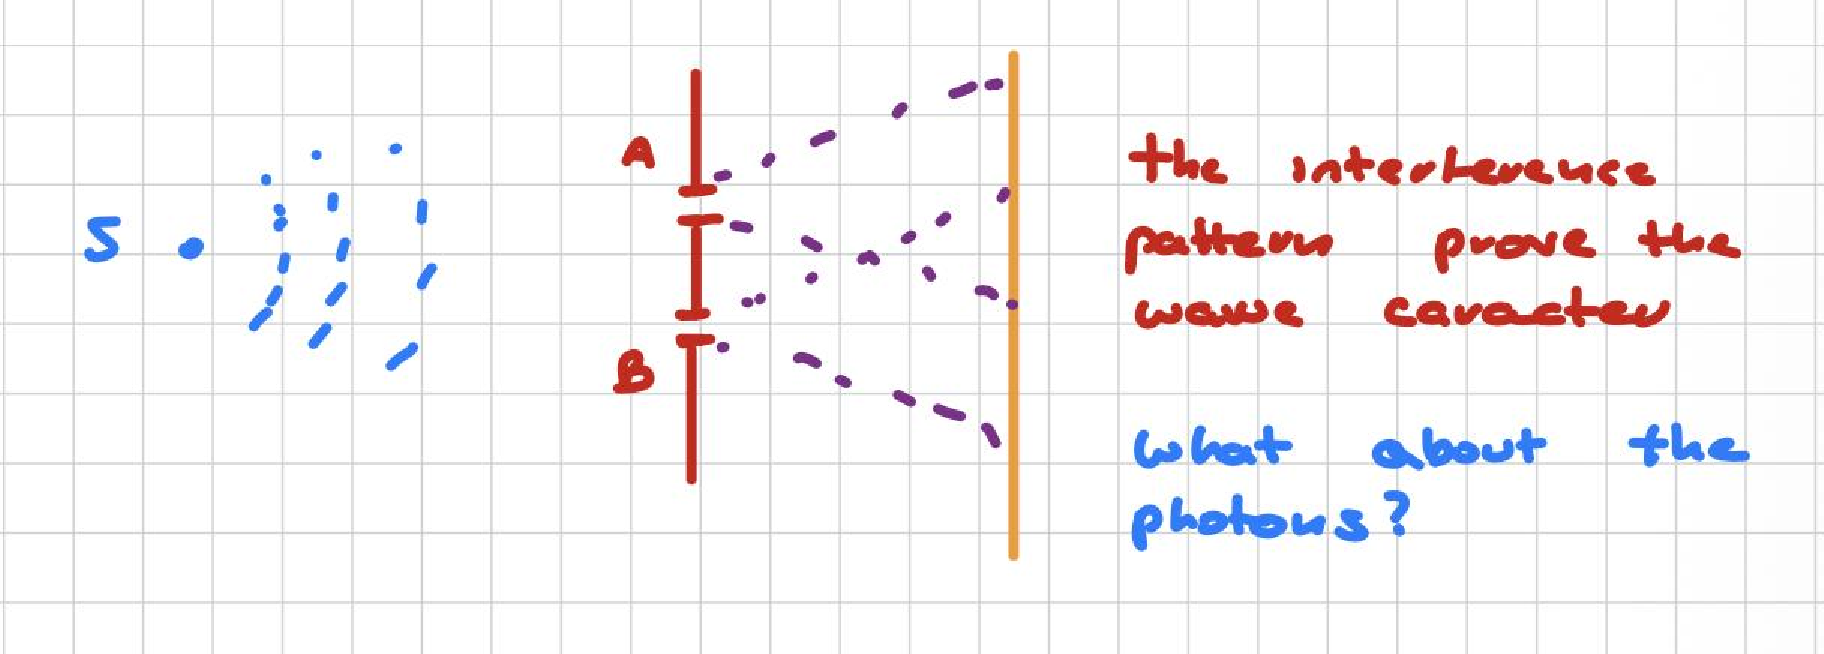
\includegraphics[width=0.8\textwidth]{images_in_pdf/1-/Grafico_1.pdf} 
\end{figure}

Now let us gradually decrease the light intensity so that, effectively, only one photon is sent at a time. By increasing the exposure time, the same interference pattern is still built up on the screen, one detection event after another. 

Now suppose we close one of the two holes, so that we obtain the diffraction pattern associated with hole $A$ or hole $B$ alone.
\begin{figure}[H]       
    \centering            
    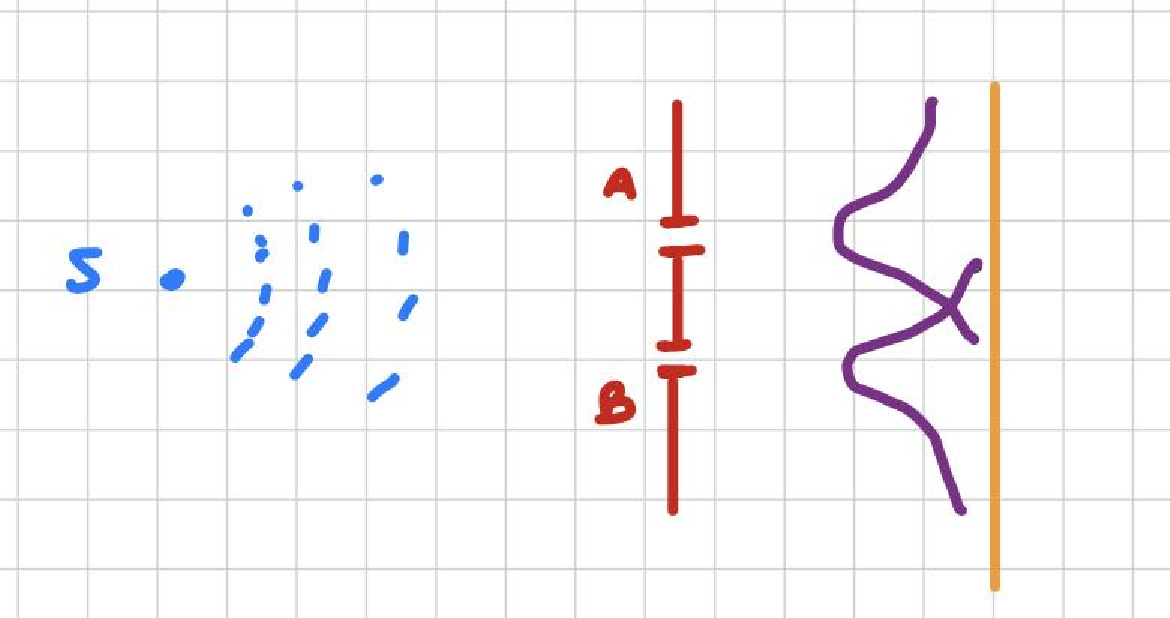
\includegraphics[width=0.8\textwidth]{images_in_pdf/1-/Grafico_2.pdf} 
\end{figure}

If we assume that $50\%$ of the photons go through $A$ and the remaining $50\%$ go through $B$, then we would expect the observed distribution to be the sum of the two single-slit diffraction patterns. However, this is not what happens in the double-slit experiment: \hl{the presence of both slits together produces an \textbf{interference pattern} that cannot be reproduced by simply adding the two single-slit intensities.} In classical language, one would say that the alternatives $A$ and $B$ are not sufficient to describe the phenomenon. In quantum mechanics, \hl{the correct description is a coherent \textbf{superposition} of the two paths rather than a classical mixture.}

We now modify the experiment by introducing a Mach-Zehnder interferometer, which is composed of:
\begin{itemize}
    \item two semi-transparent mirrors, $S_1$ and $S_4$;
    \item two normal mirrors, $S_2$ and $S_3$;
    \item two detectors, $D_1$ and $D_2$.
\end{itemize}
\begin{figure}[H]\label{1-mach-zehnder}   
    \centering            
    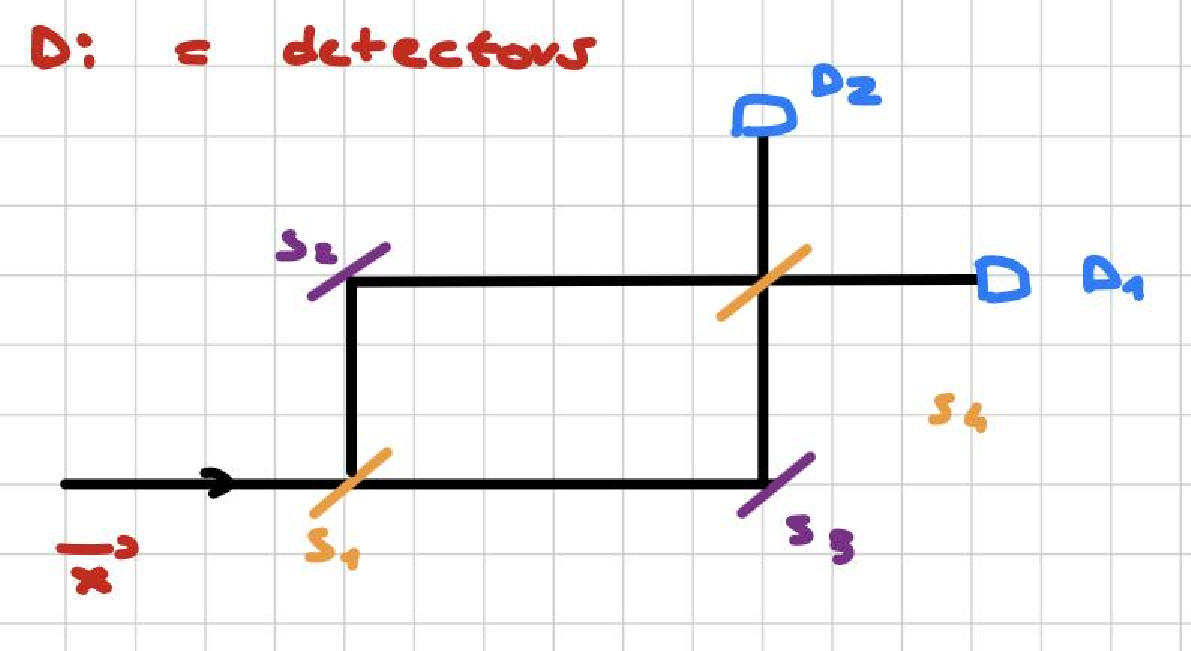
\includegraphics[width=0.8\textwidth]{images_in_pdf/1-/Grafico_3.pdf} 
\end{figure}

The beam is split at $S_1$ into two paths, reflected by $S_2$ and $S_3$, and finally recombined at $S_4$. If the interferometer is perfectly balanced, each arm carries half of the incident field amplitude and each detector receives $25\%$ of total radiation.
\begin{itemize}
     \item Path A
     \[S_1 \to S_2 \to S_4 \hspace{1.5cm}\frac{1}{2}\cdot  E_0 \cdot \cos(\omega t + \phi_1)\]
     \item Path B
     \[S_1 \to S_3 \to S_4 \hspace{1.5cm} \frac{1}{2} E_0 \cdot \cos(\omega t + \phi_2)\]
\end{itemize}

Denoting the phases accumulated along the two paths by $\phi_1$ and $\phi_2$, the two contributions at the output interfere and we measure the time average on a sufficiently long period of time:
\begin{itemize}
\item Intensity incident on $S_1$: 
\[C \cdot E^2(x,t) \implies I = C \cdot E_0^2 \cdot \braket{\cos^2(\omega t)} \propto \frac{1}{2} E_0^2\]
Where $C$ is a normalization constant.
\item Intensity incident on $D_1$:
\[I_{D_1} = C \cdot E_0^2 \cdot \braket{[\cos(\omega t + \phi_1)+\cos(\omega t + \phi_2)]^2}
= \frac{1}{2} I_0 \cdot \biggr(1+\cos(\Delta \phi)\biggr) \hspace{1cm} \Delta \phi = \phi_1-\phi_2\]
\end{itemize}

But the total intensity is given by:
\[I_{tot} = I_{D_1} + I_{D_2}\]

So we obtain:
\begin{equation}
\begin{cases}
    I_{D_1} = \frac{I_0}{2}\bigl(1+\cos\Delta\phi\bigr)\\
    I_{D_2} = \frac{I_0}{2}\bigl(1-\cos\Delta\phi\bigr)
\end{cases}
\end{equation}

where $I_0$ is the input intensity. Equivalently,
\begin{equation}
\begin{cases}
I_{D_1}=I_0\cos^2\!\left(\frac{\Delta\phi}{2}\right)\\
I_{D_2}=I_0\sin^2\!\left(\frac{\Delta\phi}{2}\right)
\end{cases}
\end{equation}

Thus, by changing the relative phase, one can continuously modulate the output intensities and obtain either constructive or destructive interference. In particular, if $\Delta\phi=0$, all the intensity exits through one detector, while the other one receives no light.

If we insert a thin glass plate in one arm of the interferometer, the optical path length changes and a phase shift is introduced. For a plate of thickness $d$ and refractive index $n$, the additional phase is
\[
\delta\phi = k_0(n-1)d = \frac{2\pi}{\lambda_0}(n-1)d,
\]

where $\lambda_0$ is the wavelength in vacuum. Even a small change in phase is enough to redistribute the counts between $D_1$ and $D_2$.

\question{Now send one photon at a time through the interferometer: should the counts at $D_1$ and $D_2$ be equal?}
{The answer is no. Because the two probability amplitudes interfere, the detection probabilities still depend on the relative phase $\Delta\phi$.} 


\calloutwarn{In the quantum description, the photon cannot be assigned a definite classical trajectory through path $A$ or path $B$. Instead, the state is described by a coherent superposition of the two paths, which is what gives rise to interference.}

\question{Returning to the Young experiment, suppose we place two detectors after the two slits $A$ and $B$: \textbf{should they click together?}}{%
\begin{figure}[H]       
    \centering            
    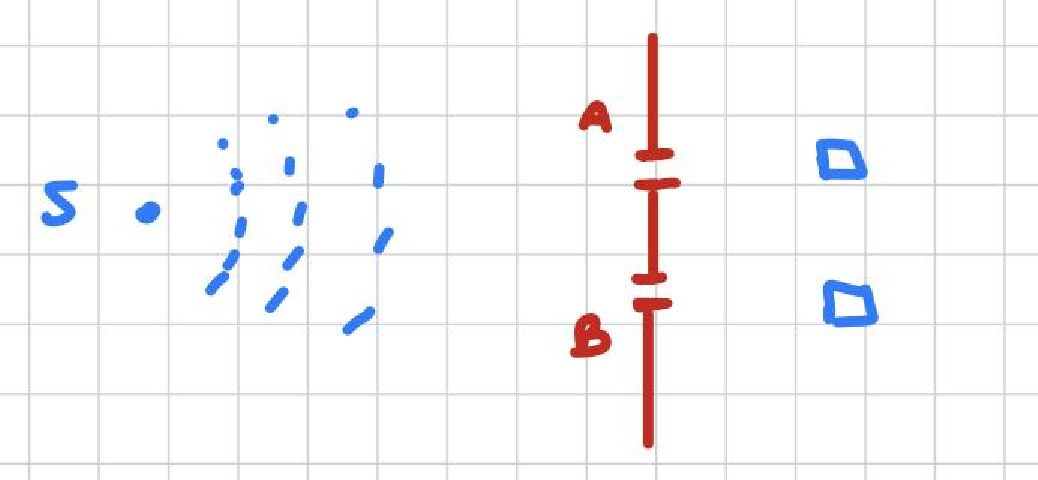
\includegraphics[width=0.5\textwidth]{images_in_pdf/1-/Grafico_4.pdf} 
\end{figure}

The answer is no. A single photon cannot be split into two independent detection events. Repeating the experiment many times, one finds that each photon is detected by one detector only and, on average, the counts are distributed according to the measurement probabilities $50 \%$  clicks on $D_1$ and  $50 \%$ clicks on $D_2$. \textbf{The presence of detectors reveals which path the photon takes, and this information eliminates the interference pattern}. In other words, \textbf{the act of measurement destroys the coherence} between the two possible paths, so they can no longer interfere.%
}

So to summarize:
\begin{enumerate}
    \item Interference fringes are observed even when photons are sent one at a time. This is often summarized by Dirac's remark that \say{each photon interferes only with itself, interference between photons does not occur} (We will see that the second remark is false).
    \item In the double-slit experiment, the photon is not correctly described as going through either slit $A$ or slit $B$ in a classical sense. The proper quantum description is a superposition of the two alternatives.
    \item A measurement that reveals which path the photon has taken destroys the coherence between the two paths, so interference can no longer be observed.
\end{enumerate}

\section{Polarized states}\label{sec:2-polarized-states}
Let us consider a monochromatic plane wave propagating along the $\hat{z}$ axis:
\begin{figure}[H]       
    \centering            
    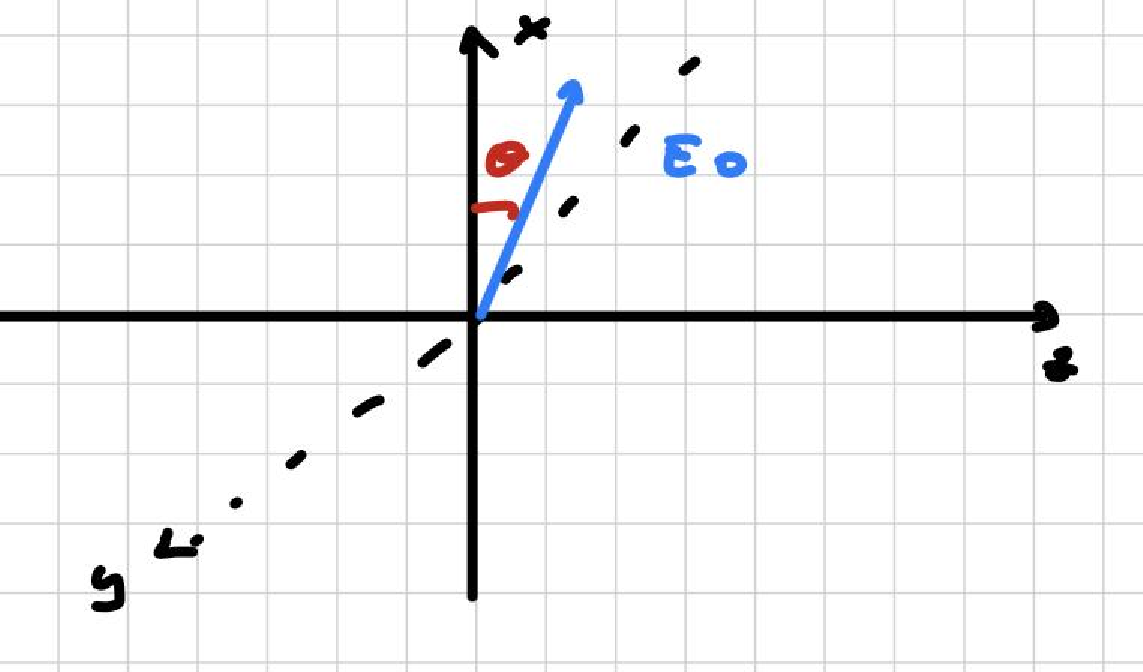
\includegraphics[width=0.8\textwidth]{images_in_pdf/2-/Grafico_5.pdf} 
\end{figure}

$E_z = 0$, since the wave propagates along $\hat{z}$ and the electric field is transverse. The field components can be written as:
\begin{equation}
\begin{cases}
    E_x(z,t) = E_{0,x} \cos(kz - \omega t + \phi_1)\\
    E_y(z,t) = E_{0,y} \cos(kz - \omega t + \phi_2)
\end{cases}
\end{equation}

We parametrize the amplitudes as:
\begin{equation}
\begin{cases}
    E_{0,x} = E_0 \cos\theta\\
    E_{0,y} = E_0 \sin\theta
\end{cases}
\end{equation}

Using the complex representation $\left(\cos\alpha = \Re\{{e^{i\alpha}}\}\right)$, the electric field can be written as:
\[
\vec{E}(z,t) = \Re \left\{ E_0 \cdot e^{\phi_1}\cdot  \left( \cos\theta\, \hat{x} + e^{i\Delta\phi}\sin\theta\, \hat{y} \right) e^{i(kz - \omega t)} \right\}
\]
where $\Delta\phi = \phi_2 - \phi_1$ is the relative phase between the two components. The overall phase $e^{\phi_1}$ is not physically relevant.

The vector:
\begin{equation}\label{eqn:2-polarization-vector}
\vec{e}_{\theta,\phi} = \cos\theta\, \hat{x} + e^{i\Delta\phi}\sin\theta\, \hat{y}
\end{equation}

is called the \textbf{polarization vector} and fully characterizes the polarization state of the wave.

Different choices of $\theta$ and $\Delta\phi$ correspond to different polarization states:

\begin{enumerate}
    \item If $\Delta \phi = 0$ (or $\pi$), the field components oscillate in phase and the wave is \textbf{linearly polarized}. In particular:
    \begin{itemize}
        \item $\theta = 0 \Rightarrow$ polarization along $\hat{x}$;
        \item $\theta = \frac{\pi}{2} \Rightarrow$ polarization along $\hat{y}$.
    \end{itemize}
    
    \item If $\theta = \frac{\pi}{4}$ and $\Delta\phi = \pm \frac{\pi}{2}$, the wave is \textbf{circularly polarized}, with polarization vectors:
    \begin{equation}\label{eqn:2-circular-polarization}
        \vec{e}_{\sigma^{\pm}} = \frac{1}{\sqrt{2}}(\hat{x} \pm i \hat{y})
    \end{equation}
    
    \item In the general case, the wave is \textbf{elliptically polarized}.    
\end{enumerate}

\hl{In quantum mechanics, the polarization state of a single photon is described by a two-dimensional complex Hilbert space}. Any polarization state can be written as a superposition of two orthogonal basis states, for example $(\hat{x}, \hat{y})$ or the circular basis. This representation is not unique, but any pair of orthogonal states spans the space.

The key point is that polarization provides a fundamental and controllable degree of freedom, widely used in both classical and quantum optical experiments.

\section{Spin injection}\label{sec:spin-injection}

\subsection{Introduction}

In this section we discuss how light can be used to manipulate spins inside a solid-state material.

We start by considering a semiconductor and the energy dispersion around the center of the Brillouin zone, $\Gamma \equiv (0,0,0)$, where the band structure is typically divided into two main parts:
\begin{itemize}
    \item \textbf{Conduction band}: an $s$-type antibonding band.
    \item \textbf{Valence band}: a $p$-type bonding band, which is split into three sub-bands, namely heavy holes (HH), light holes (LH), and the split--off (SO) band, due to spin--orbit coupling.
\end{itemize}
The HH and LH bands are degenerate at the Brillouin zone center, while the SO band is separated by the spin--orbit interaction.

Let us assume the following conditions:
\begin{enumerate}
    \item the optical transitions are dipole allowed;
    \item a four-band model is sufficient near $k \simeq 0$;
    \item subsidiary minima at $k \neq 0$ can be neglected.
\end{enumerate}

\question{From the band structure alone, can we conclude that the material is magnetic?}{The answer is no, because in the absence of an external magnetic field the electronic states are spin degenerate. In particular, the conduction band states are doubly degenerate, corresponding to spin-up $(m_s=+1/2)$ and spin-down $(m_s=-1/2)$.}

\subsection{Optical spin orientation}

\subsubsection{Light can carry angular momentum}
A net spin population can be created by using circularly polarized light. This mechanism is widely exploited in quantum technologies, such as spin-photon interfaces, and in spintronics applications such as spin-LEDs and spin lasers.

\calloutinfo{Circularly polarized light carries angular momentum along the propagation direction. In particular, right- and left-handed circular polarizations, usually denoted by $\sigma^+$ and $\sigma^-$, correspond to angular momentum $\pm \hbar$, respectively, depending on the handedness convention.}

A circularly polarized electric field can be viewed as the superposition of two orthogonal components, $E_x$ and $E_y$, oscillating with a relative phase shift of $\lambda/4$.
\begin{figure}[H]       
    \centering            
    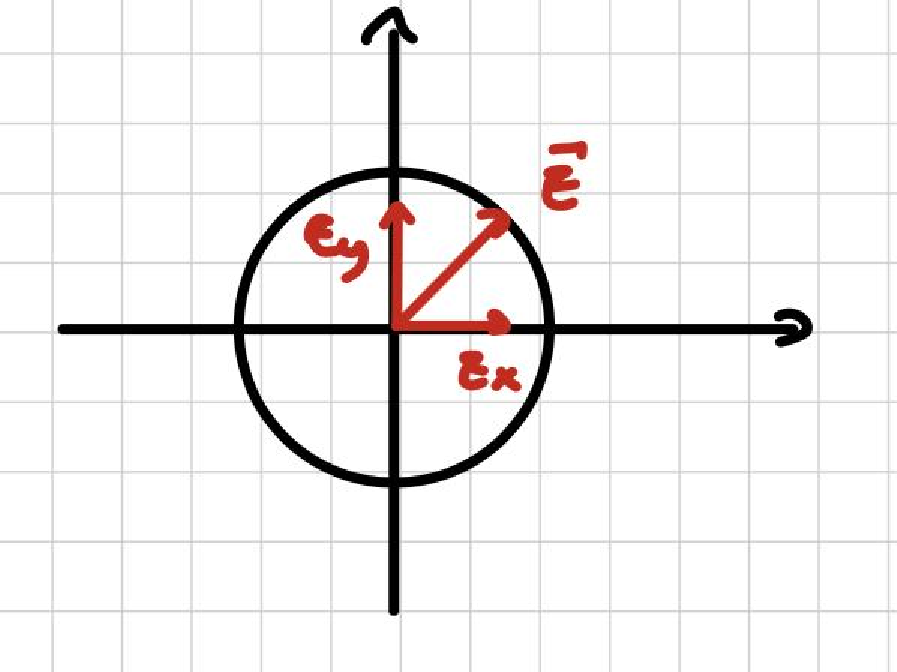
\includegraphics[width=0.8\textwidth]{images_in_pdf/3-/Grafico_6.pdf} 
\end{figure}

When a single electron absorbs circularly polarized light, the response is an acceleration caused by the rotating electric field (circular orbits). The connection with angular momentum can be understood by comparing the power delivered by the electromagnetic field with the power associated with a torque:
\[
P_1 = \odv{\varepsilon}{t}, \qquad P_2 = \tau \omega,
\]

where $\tau$ is the torque and $\omega$ the angular frequency. Since torque is the rate of change of angular momentum on average, one has
\[
P_1 = P_2 \implies \odv{\varepsilon}{t} = \omega \odv{L}{t},
\]

so that the absorbed angular momentum per quantum of energy is
\[
\varepsilon = \hbar \omega \implies L = \frac{\varepsilon}{\omega} = \hbar.
\]

Therefore, each circularly polarized photon carries angular momentum $\pm \hbar$, with the sign determined by the helicity.
\begin{figure}[H]       
    \centering            
    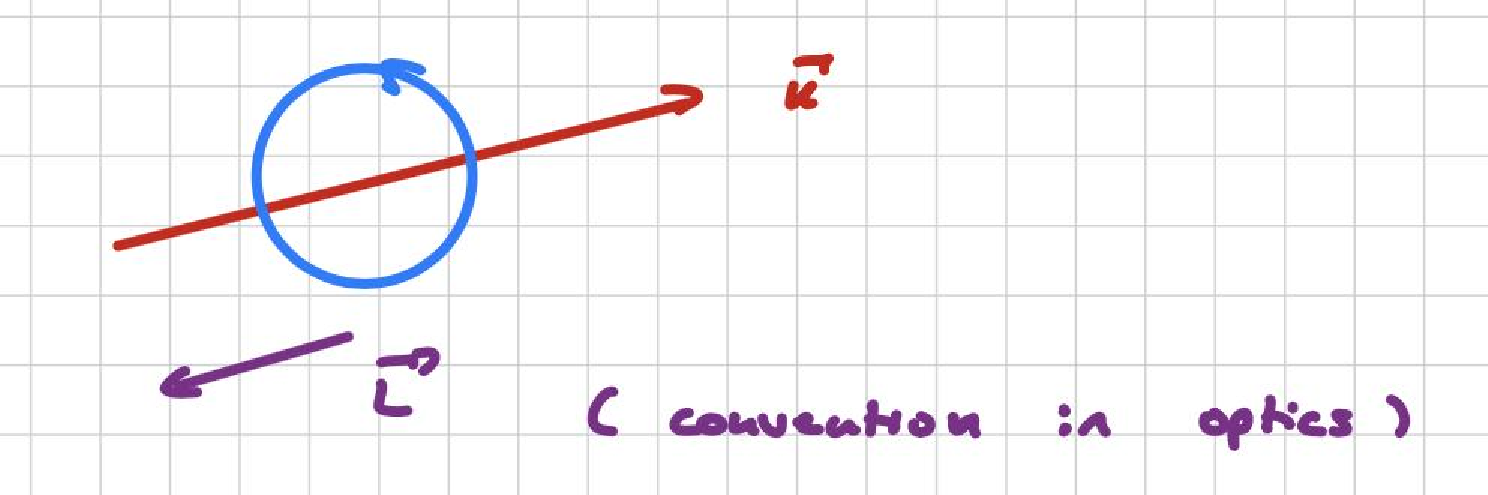
\includegraphics[width=0.8\textwidth]{images_in_pdf/3-/Grafico_7.pdf} 
\end{figure}

For this reason, we distinguish two \textbf{helicity states} of circularly polarized light:
\begin{itemize}
    \item $\ket{L}$ transfers angular momentum to the target as if the photon spin were aligned with the propagation direction;
    \item $\ket{R}$ reverses the handedness and transfers angular momentum with opposite sign.
\end{itemize}

\subsubsection{Transition rates}
In the semiconductor:
\begin{itemize}
    \item The conduction band is $s$-like, so $\ell=0$ and the states are characterized by $j=\ell+s = 1/2$.
    
    \item The valence band is $p$-like and, after including spin-orbit coupling, is described by the total angular momentum $j$, with $\ell-s \leq j \leq |\ell+s| \implies j = \frac{1}{2},\frac{3}{2}$: the states split into $j=3/2$ (HH and LH) and $j=1/2$ (SO).
\end{itemize} 
The corresponding magnetic quantum number satisfies $-j \leq m_j \leq +j$ along the quantization axis, which is taken to be the propagation direction.
\begin{figure}[H]       
    \centering            
    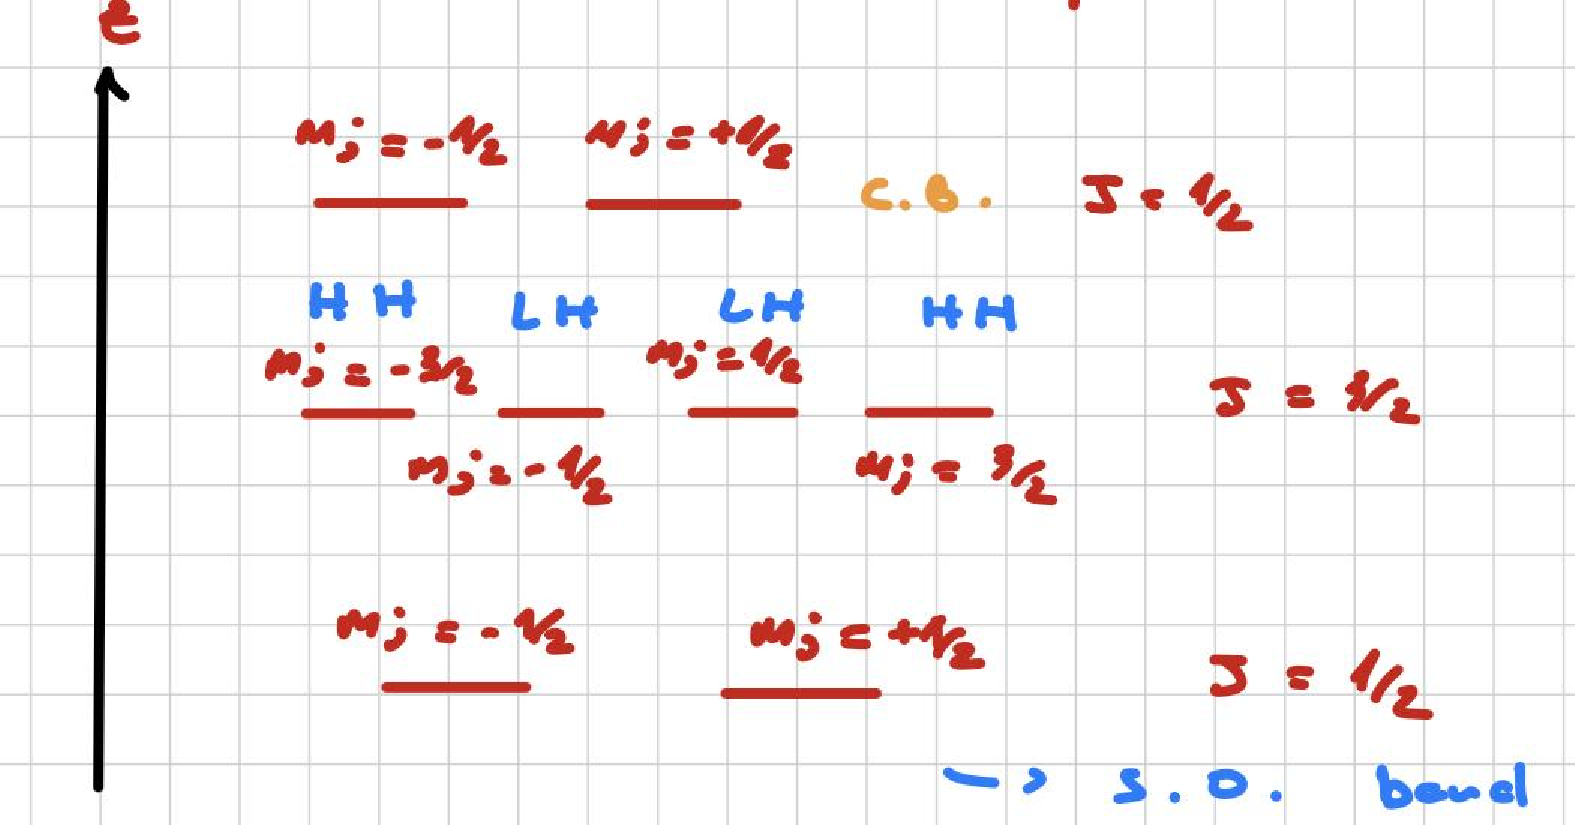
\includegraphics[width=0.8\textwidth]{images_in_pdf/3-/Grafico_8.pdf} 
\end{figure}

To compute the transition rate, we evaluate the matrix element
\begin{equation}\label{eqn:3-radiative-transition-matrix-element}
M = \bra{\psi_f}\hat{H}_{\text{int}}\ket{\psi_i}
\end{equation}

where, in the electric dipole approximation,
\[
\hat{H}_{\text{int}} = -\vec{d}\cdot \vec{E}_0,
\qquad
\vec{d} = -e\vec{r},
\]

with $\vec{r}=\hat{x}+\hat{y}+\hat{z}$ being the position vector of the electron and $\vec{E}_0$ the electric field amplitude.

The wave function can be factorized into a radial part and an angular part,
\[
\psi_{n,\ell,m}(r,\theta,\phi) = R_{n,\ell}(r)\,Y_{\ell,m}(\theta,\phi),
\]

so that the matrix element is obtained by integrating over the full spatial coordinates.
\[
M = \int_0^{+\infty} \d{r} \cdot \int_0^{\pi} \d\theta \cdot \int_0^{2\pi} \d\phi \cdot \psi_f^*\cdot  \hat{H} \cdot \psi_i\cdot r^2 \sin^2(\theta)
\]

The dot product between the dipole operator and the electric field is proportional to:

\begin{equation}
\vec{e}_{\sigma^{\pm}} = \frac{1}{\sqrt{2}}\cdot (\hat{x} \pm i\hat{y})
\implies 
\vec{e}_{\sigma^{\pm}} \cdot \vec{r} =
\frac{1}{\sqrt{2}}\cdot (x \pm i y)
\end{equation}

Then, in polar coordinates:
\begin{equation}
\begin{cases}
    x=r\cos\phi\\[0.5ex]
    y=r\sin\phi
\end{cases}
\implies
x \pm i y = r(\cos\phi \pm i \sin\phi) 
\equiv r e^{\pm i\phi}
\end{equation}

The angular part of the matrix element is therefore proportional to:
\[
M_{\sigma^{\pm}} \propto \int_0^{2\pi} d\phi\cdot  Y_{\ell',m'}^*(\theta,\phi) \cdot e^{\pm i \phi} \cdot Y_{\ell,m}(\theta,\phi) \propto \int_0^{2\pi} d\phi\cdot  e^{-im'\phi} \cdot e^{\pm i \phi} \cdot e^{im\phi} \ne 0
\]

which is nonzero only if the selection rule
\begin{equation}\label{eqn:3-dipole-selection-rule}
\Delta m_\ell = \pm 1
\end{equation}

is satisfied. Since spin cannot change under electric dipole transitions, the condition on $m_\ell$ results in one on $m_j$; circularly polarized light couples only to specific transitions:
\begin{itemize}
    \item $m_j' = m_j + 1, \Delta m_j = +1 \iff \sigma^+$ transition;
    
    \item $m_j' = m_j - 1, \Delta m_j = -1 \iff \sigma^-$ transition.
\end{itemize}
For this reason, only a restricted set of optical transitions is allowed.

\begin{figure}[H]       
    \centering            
    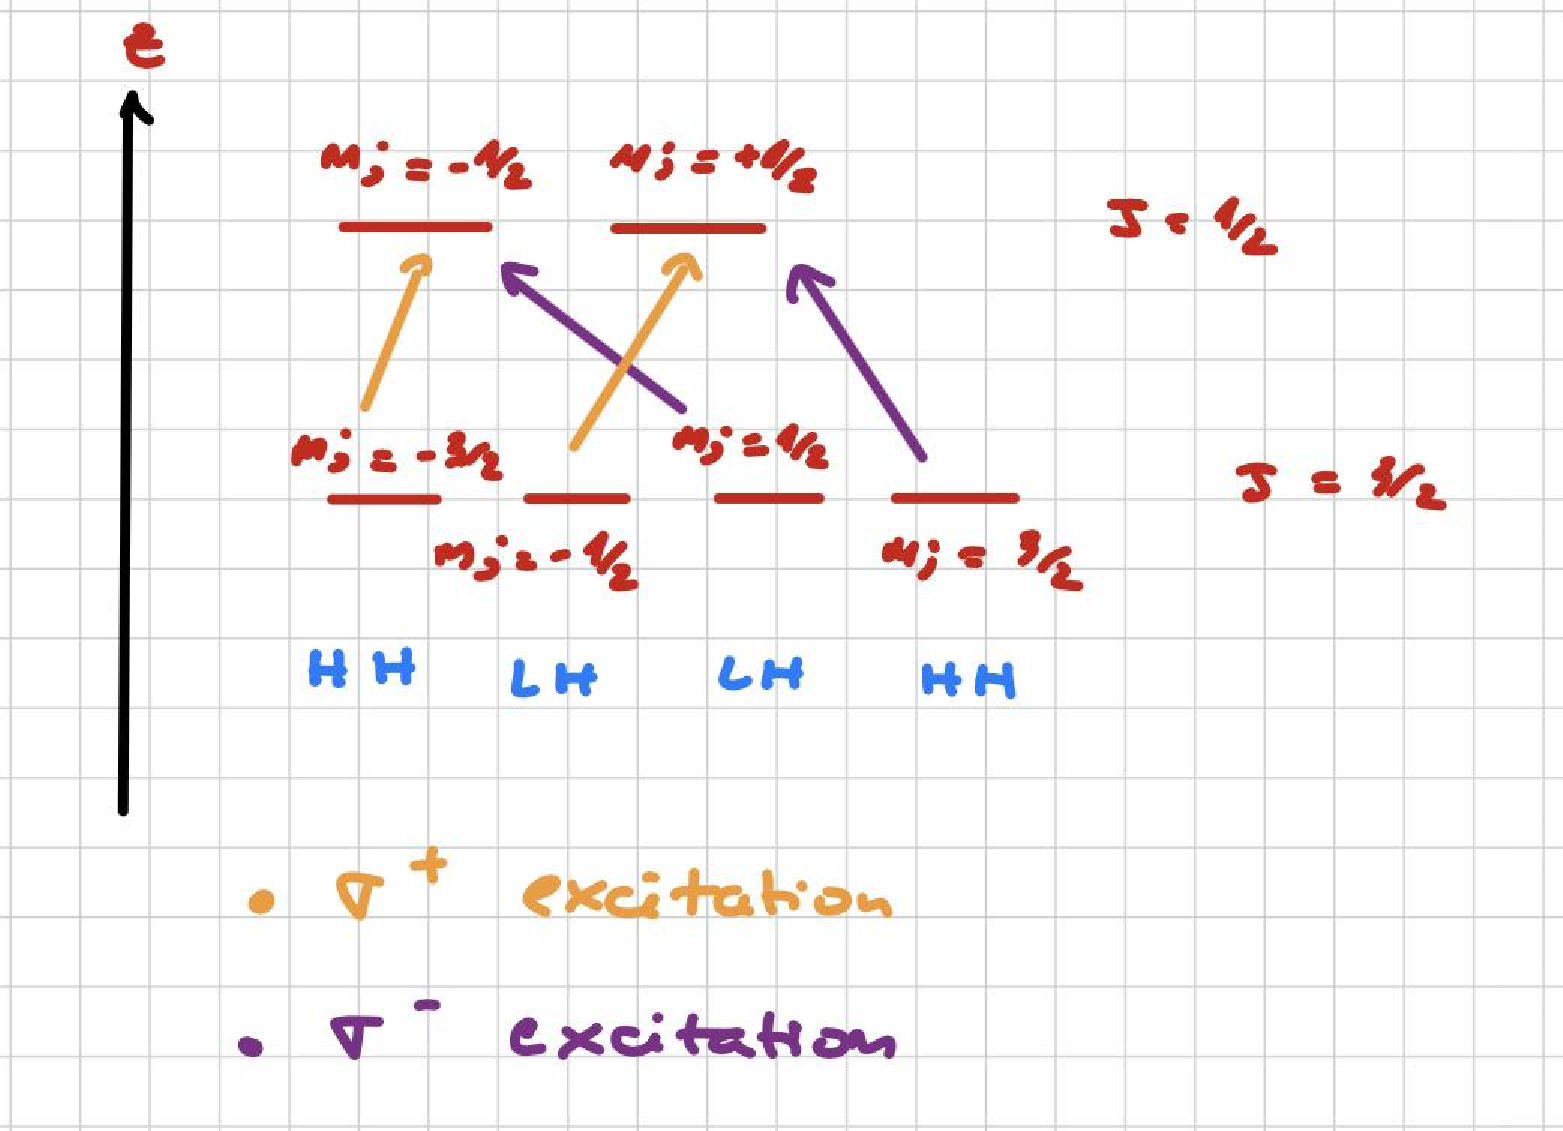
\includegraphics[width=0.8\textwidth]{images_in_pdf/3-/Grafico_9.pdf} 
\end{figure}

Using Fermi's golden rule, stating the transition rate is proportional to $|M|^2$, can be shown that:
\[
|M_{HH}|^2 = 3|M_{LH}|^2.
\]

This imbalance means that \hl{transitions involving heavy--hole states are favored over light--hole states}.
\begin{figure}[H]       
    \centering            
    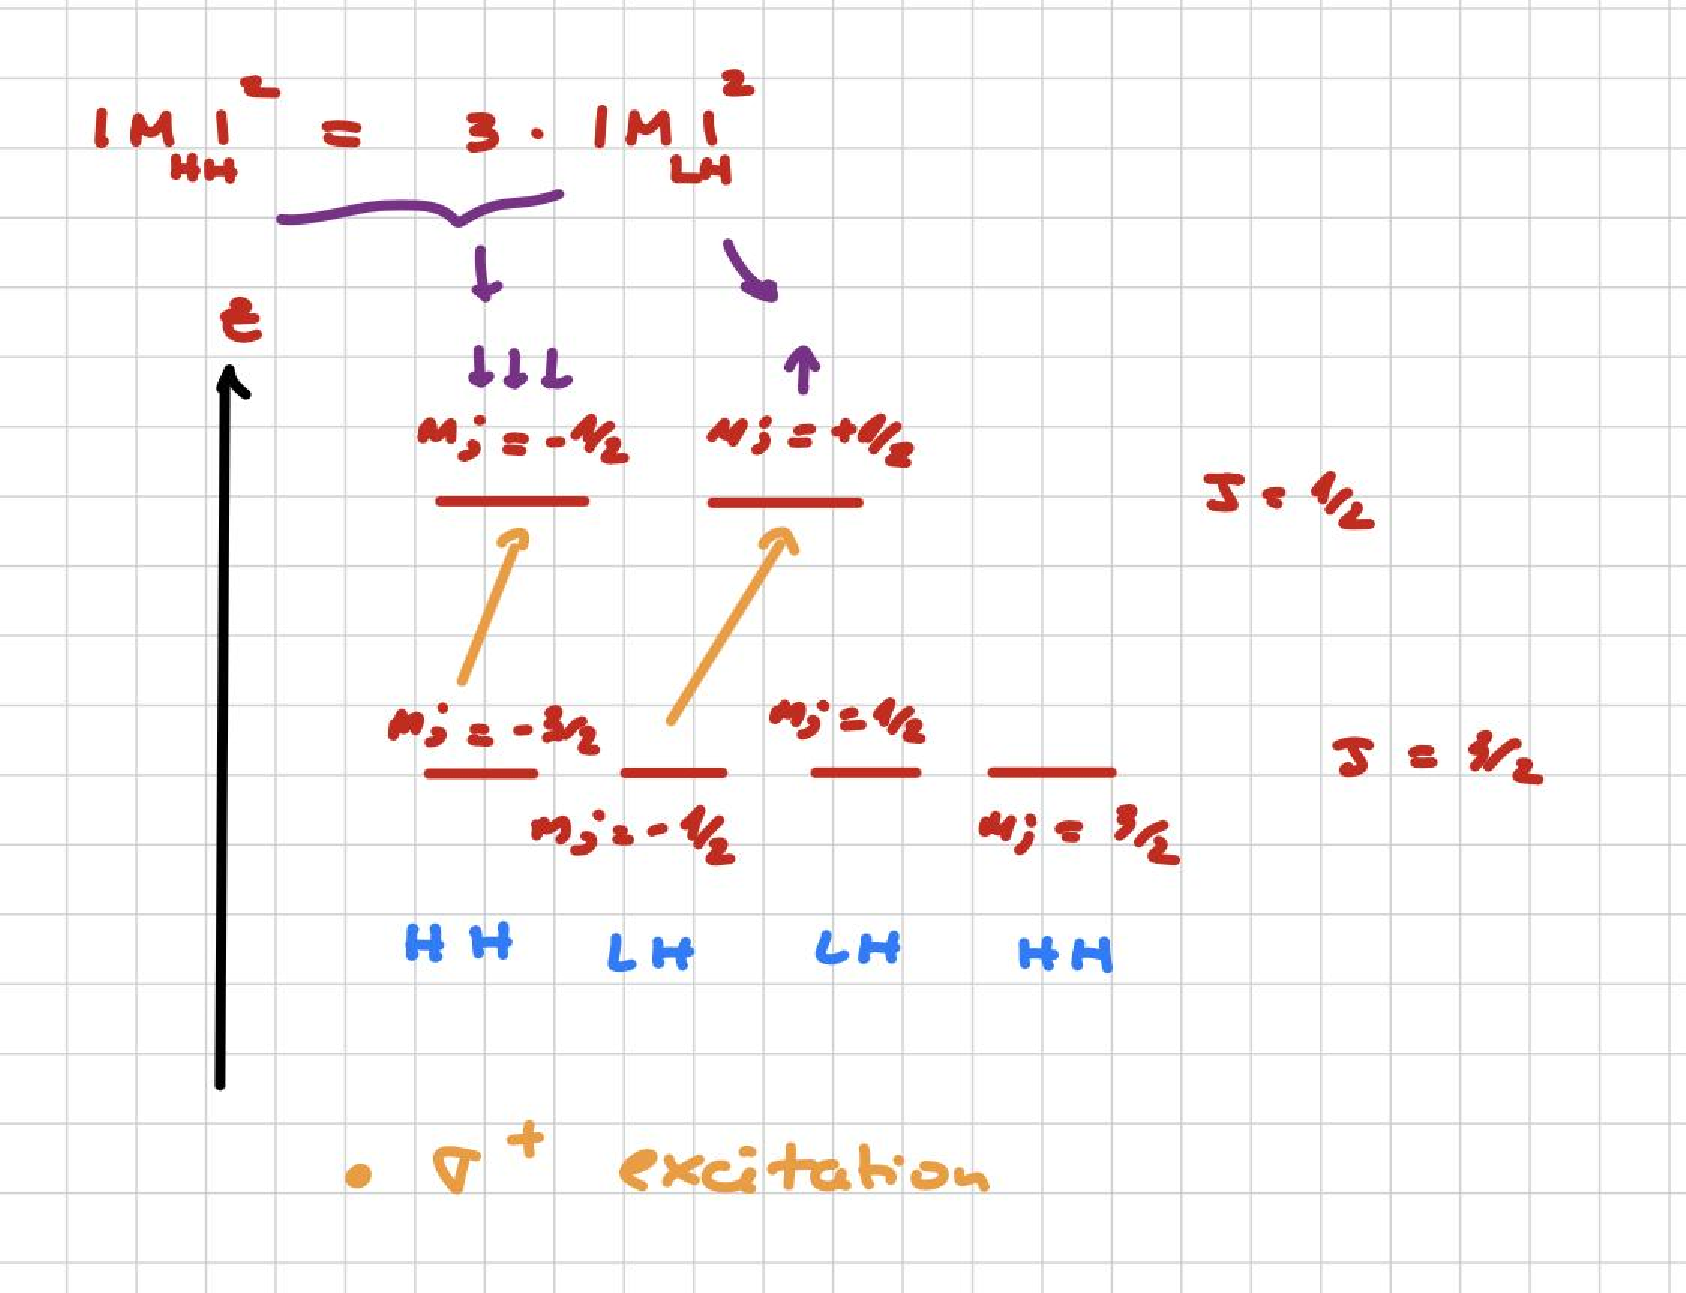
\includegraphics[width=0.8\textwidth]{images_in_pdf/3-/Grafico_10.pdf} 
\end{figure}

As a consequence, the excited carrier population becomes spin polarized. 
In the simplest bulk model, the resulting electron spin polarization is
\begin{equation}\label{eqn:3-spin-polarization}
P_s = \frac{N(+1/2)-N(-1/2)}{N(+1/2)+N(-1/2)} = 
\frac{1-3}{1+3}= -50\%
\end{equation}

\calloutinfo{The same idea applies to holes, but their spin polarization is usually much less robust because spin--orbit coupling in the valence band causing rapid spin relaxation. For electrons in the $s$-type ($\ell=0$) conduction band, this effect is much weaker, since the orbital angular momentum is approximately zero and therefore $\vec{L}\cdot \vec{S}$ is small.}

If the system is excited with $\sigma^+$ light and the split--off states ($\ell=1, m_\ell=0$) are also included, one finds that
\[
|M_{SO}|^2 = 2|M_{LH}|^2.
\]

\begin{figure}[H]       
    \centering            
    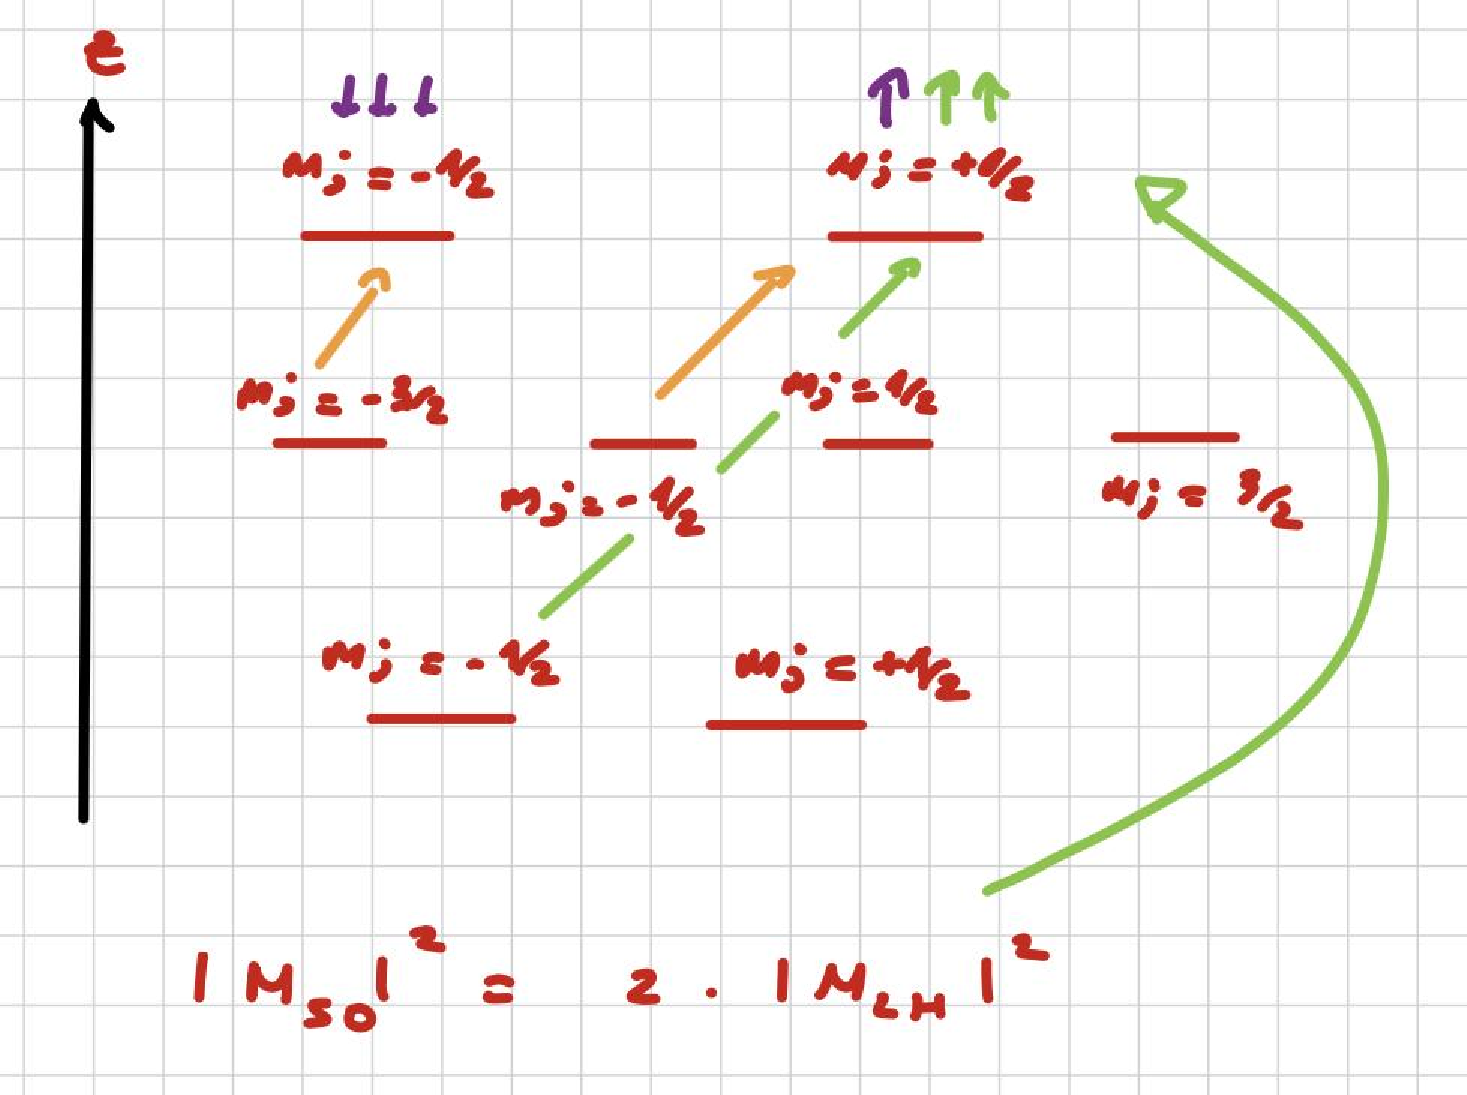
\includegraphics[width=0.8\textwidth]{images_in_pdf/3-/Grafico_11.pdf} 
\end{figure}

As a result, the electron spin polarization exhibits a clear spectral dependence. At the bandgap threshold, where the split-off band is not yet accessible, the polarization reaches its peak value of 50\%. Beyond this onset, the net polarization becomes a function of the photon energy:
\[
P_s = P_s(E=\hbar\omega).
\]
\begin{figure}[H]       
    \centering            
    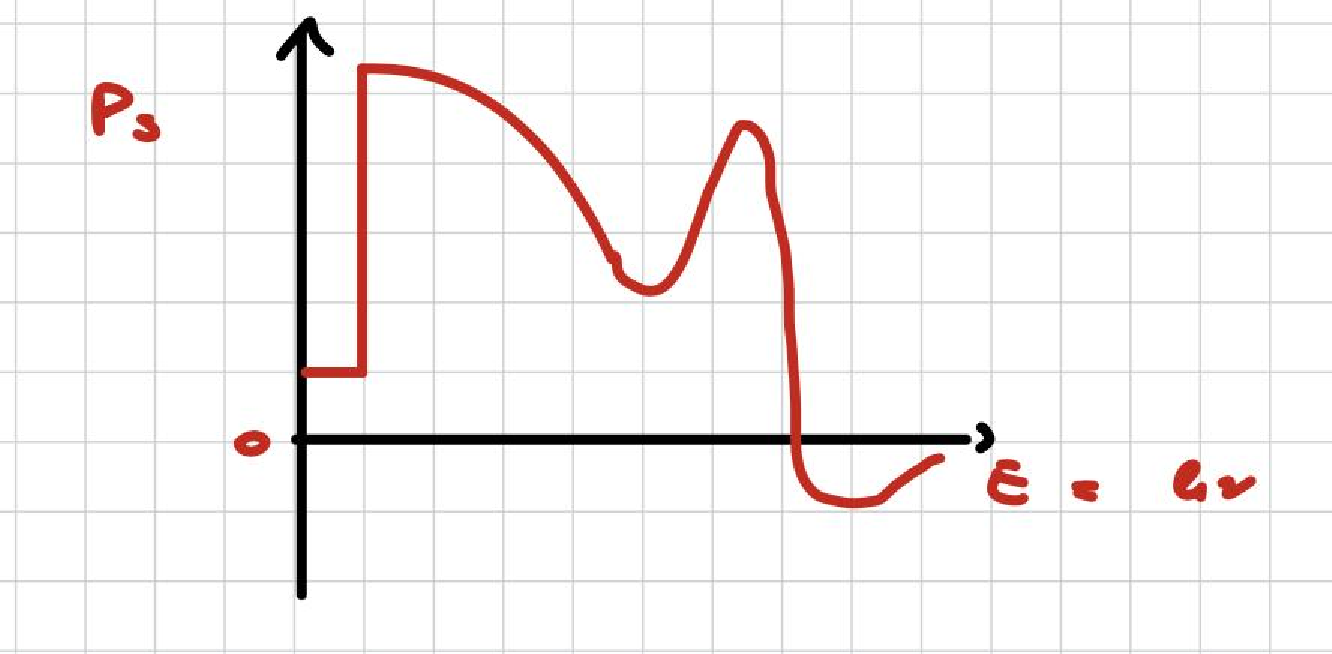
\includegraphics[width=0.8\textwidth]{images_in_pdf/3-/Grafico_12.pdf} 
\end{figure}

\calloutwarn{The split--off band becomes relevant at higher photon energies, where it drives the polarization toward smaller and even negative values. This behavior is related to the band curvature and to the density of states, which determine how many transitions contribute at each energy. Moreover, away from the center of the Brillouin zone, the HH and LH bands are no longer degenerate and their character becomes mixed, making the problem more complicated.}

\subsection{Experimental determination of spin polarization}

While analytically modeling this $P_s(E)$ behavior away from the Brillouin zone center is highly complex due to these band-mixing effects, we can experimentally determine the spin polarization by exploiting optical techniques. Since the selection rules governing absorption must also dictate the radiative recombination of spin-polarized carriers, we can rely on \textbf{circularly polarized photoluminescence} (PL) as a direct probe. By measuring the luminescence polarization, and assuming that the same transition rules remain valid for recombination:
\begin{figure}[H]       
    \centering            
    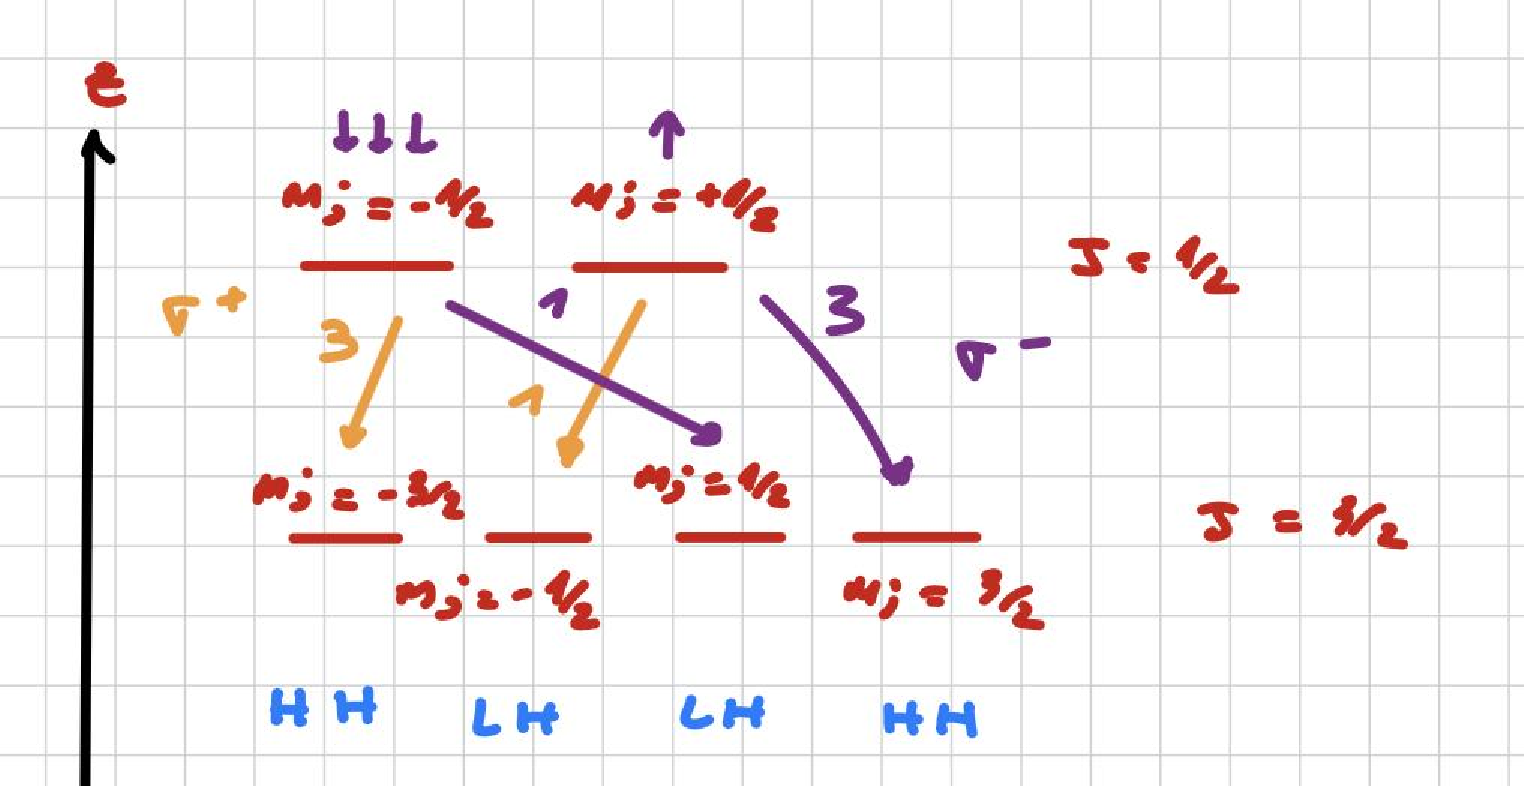
\includegraphics[width=0.8\textwidth]{images_in_pdf/3-/Grafico_13.pdf} 
\end{figure}

\[
\rho_c = \frac{I^+ - I^-}{I^+ + I^-}
= \frac{(1\cdot n_{\uparrow} + 3\cdot n_{\downarrow}) - (3\cdot n_{\uparrow} + 1\cdot n_{\downarrow})}
{(1\cdot n_{\uparrow} + 3\cdot n_{\downarrow}) + (3\cdot n_{\uparrow} + 1\cdot n_{\downarrow})}
= 25\% = -\frac{P_s}{2},
\]

where $I^\pm$ denotes the intensity of the luminescence component with helicity $\sigma^\pm$.

This shows that the maximum observable polarization in this simplified bulk picture is $25\%$, although experimentally the measured value is usually smaller.
\begin{figure}[H]       
    \centering            
    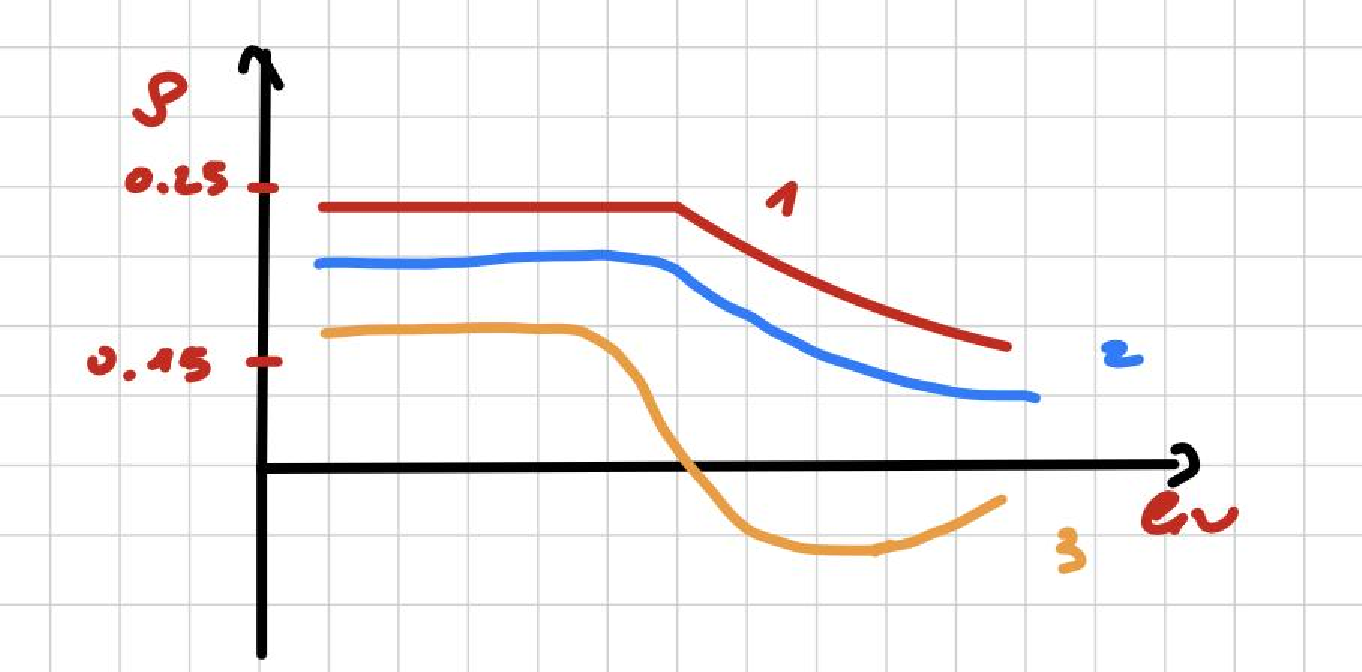
\includegraphics[width=0.8\textwidth]{images_in_pdf/3-/Grafico_14.pdf} 
\end{figure}

The reduction is caused by spin-relaxation mechanisms acting between optical excitation and recombination:
\[
\rho_c = \frac{\rho_0}{1+\tau/\tau_s},
\]

where $\rho_0$ is the polarization in the absence of spin relaxation, $\tau$ is the carrier lifetime, and $\tau_s$ is the spin-relaxation time. Thus,
\begin{itemize}
    \item if $\tau \gg \tau_s$, then $\rho_c \to 0$;
    \item if $\tau \ll \tau_s$, then $\rho_c \to \rho_0$.
\end{itemize}
The main spin-relaxation mechanisms are:
\begin{enumerate}
    \item \textbf{Dyakonov-Perel mechanism:} it occurs in crystals lacking inversion symmetry. Spin degeneracy is lifted by spin-orbit coupling, which acts as an effective magnetic field $\vec{B}_{\mathrm{eff}}$. The direction of this effective field changes randomly during scattering events, leading to spin depolarization through a sequence of random precessions. This mechanism does not occur in centrosymmetric materials such as Si or Ge.
    \item \textbf{Elliott-Yafet mechanism:} it is important in narrow-gap semiconductors. Strong spin-orbit coupling mixes spin-up and spin-down components in the wave functions, so scattering events can cause spin flips and reduce the polarization.
    \item \textbf{Bir-Aharonov-Picus mechanism:} it originates from exchange interaction between electrons and holes, which can induce electron spin flips.
\end{enumerate}

\subsection{Spin injection in low-dimensional structures}

\question{How can we improve the spin polarization?}{%
    The main limitation in the bulk case is that optical excitation generally involves both HH and LH states, which reduces the achievable polarization. A way to enhance the spin selectivity is to remove the HH-LH degeneracy using low-dimensional structures.
}

A particularly useful example is a quantum well made of alternating \ce{GaAs} and \ce{AlGaAs} layers, where the \ce{GaAs} thickness $t$ is chosen such that
\[
t \lesssim \lambda_{\mathrm{dB}},
\]
with $\lambda_{\mathrm{dB}}$ being the de Broglie wavelength of the carriers.
\begin{figure}[H]       
    \centering            
    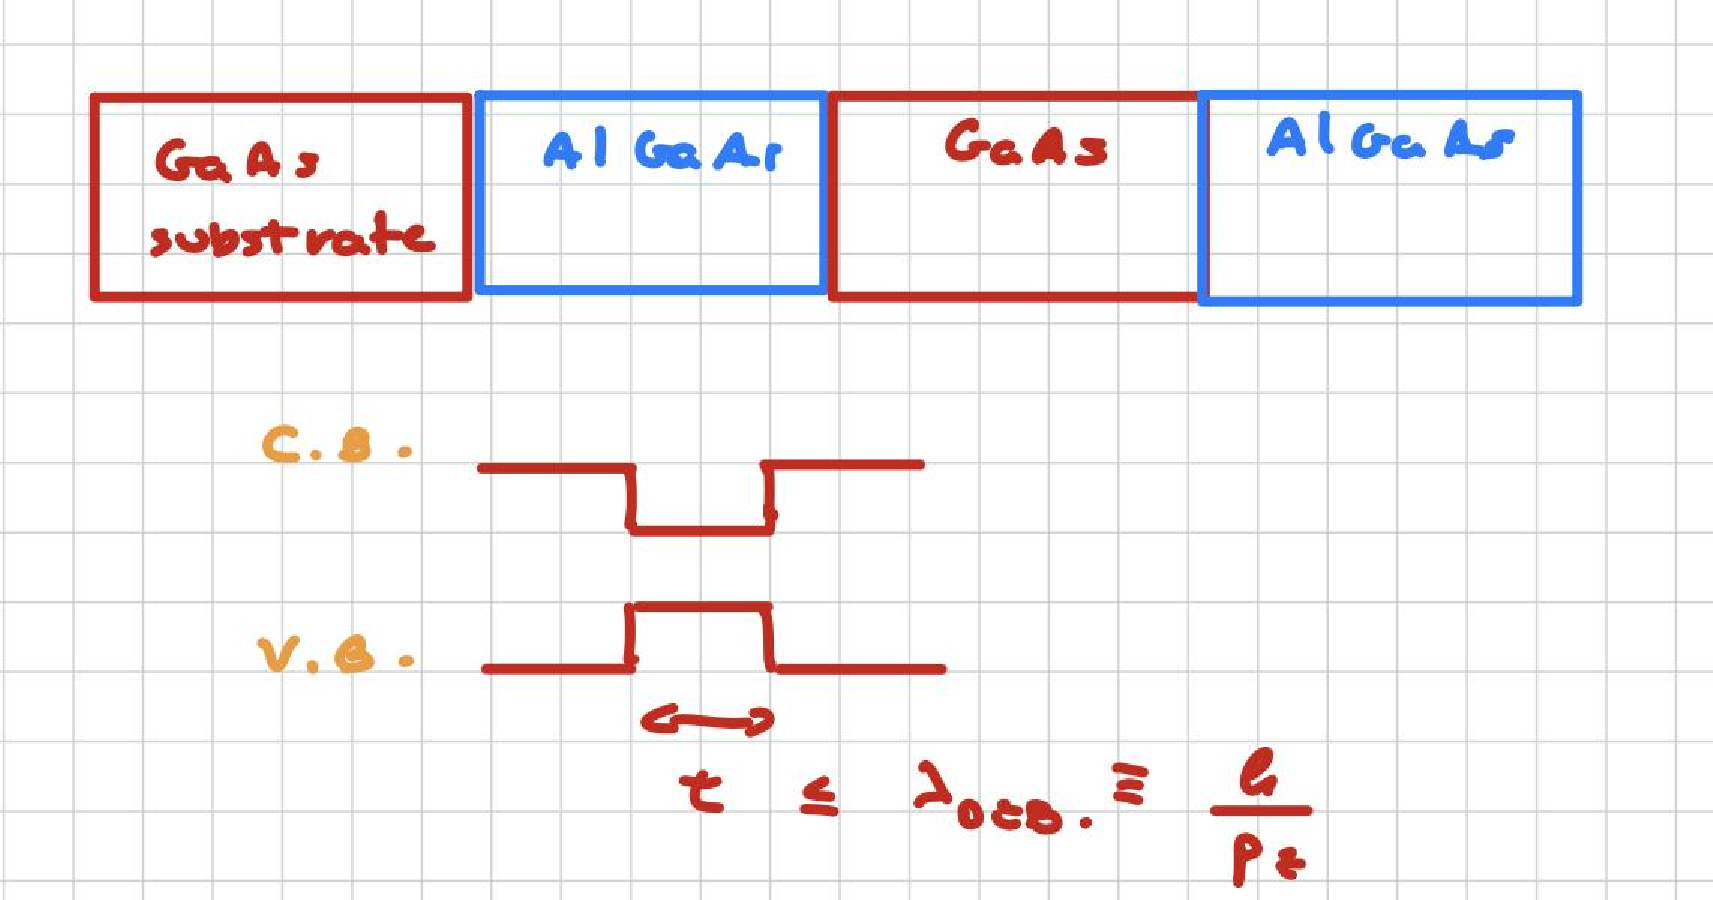
\includegraphics[width=0.8\textwidth]{images_in_pdf/3-/Grafico_15.pdf} 
\end{figure}

In this regime, quantum confinement becomes important and the system behaves approximately like a particle in a box, with discrete energy levels:
\[
E_n = \frac{\hbar^2}{2m^*}\left(\frac{n\pi}{L}\right)^2.
\]

\calloutinfo{Since the confinement energy depends on the effective mass $m^*$, it is different for HH and LH states. As a result, the two bands are split, hence the two transitions require different energies. If the system is excited with circularly polarized light in this energy window:
\[
E_g + E_{e_1} + E_{HH_1} \leq \hbar\omega \leq E_g + E_{e_1} + E_{LH_1},
\]
one can in principle obtain $100\%$ electron spin polarization.}

Here:
\begin{itemize}
    \item $E_g$ is the band gap;
    \item $E_{e_1}$ is the confinement energy of the first electron sub-band;
    \item $E_{HH_1}$ is the first confinement energy of the HH sub-band;
    \item $E_{LH_1}$ is the first confinement energy of the LH sub-band.
\end{itemize}
\begin{figure}[H]       
    \centering            
    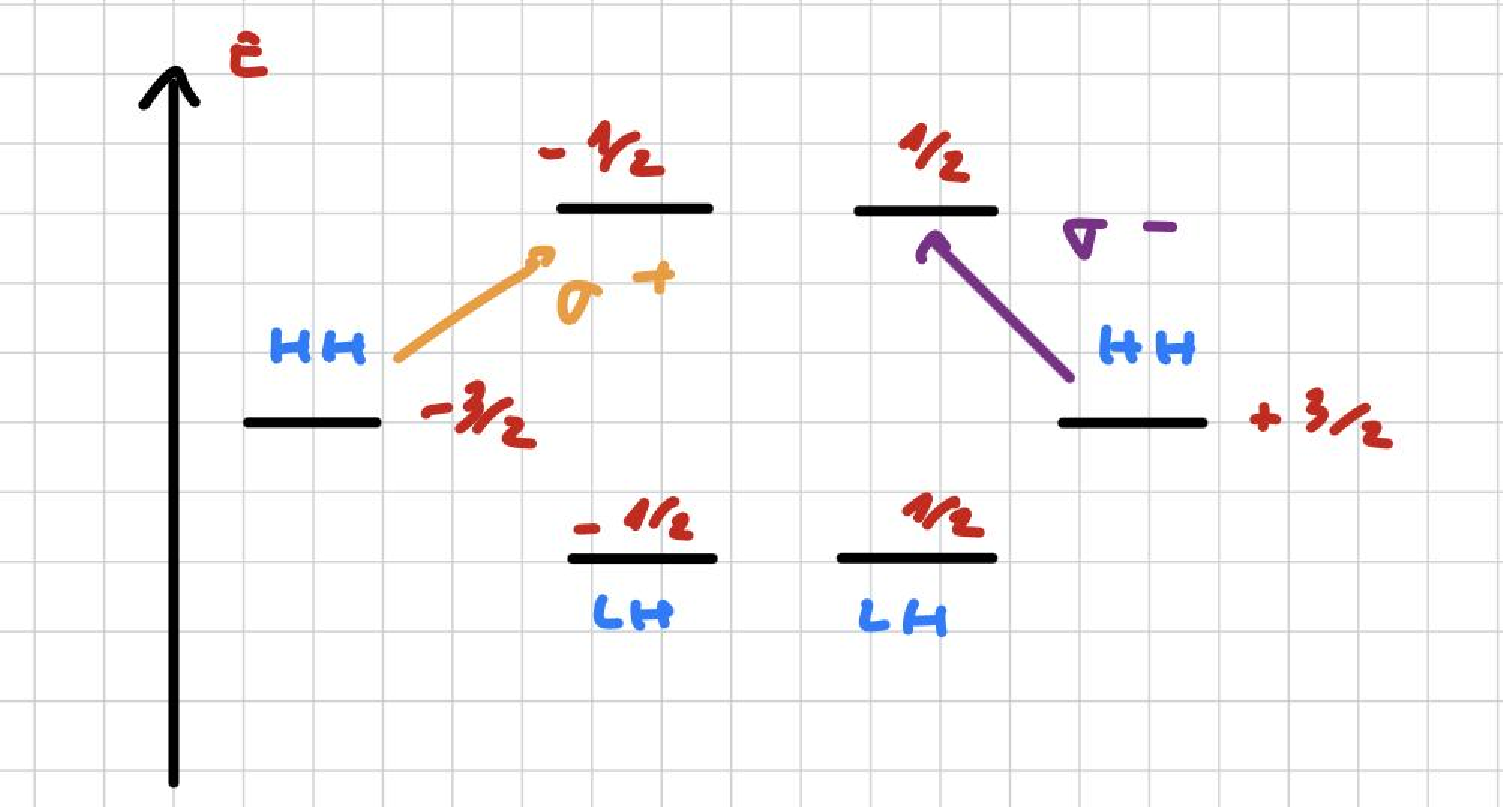
\includegraphics[width=0.8\textwidth]{images_in_pdf/3-/Grafico_16.pdf} 
\end{figure}

In this way one can reach an electron polarization degree
\[
P_c = \pm 100\%,
\]

where the sign depends on the helicity $\sigma^\pm$.

\hl{The key point is that the spin orientation is determined by the helicity of the light.}

Notice that the splitting of the valence sub-bands suppresses HH-LH mixing and also reduces spin relaxation of the holes compared with the bulk case.

\subsection{Spin quantum beat}\label{subsec:3-spin-quantum-beat}

Suppose we send circularly polarized $\sigma^+$ light pulses propagating along the $z$-axis onto a \ce{GaAs} quantum well and then apply an external magnetic field along the $x$-axis, $\vec{B}_{\mathrm{ext}} = B_{\mathrm{ext}} \hat{x}$. 

\calloutinfo{In this situation, the photoexcited spins undergo Larmor precession, so that the expectation value of the spin component along $z$, $\langle \hat{S}_z \rangle$, oscillates in time between positive and negative values. This effect is known as a \textbf{spin quantum beat}.}

\begin{figure}[H]\label{fig:3-spin-quantum-beat}
    \centering            
    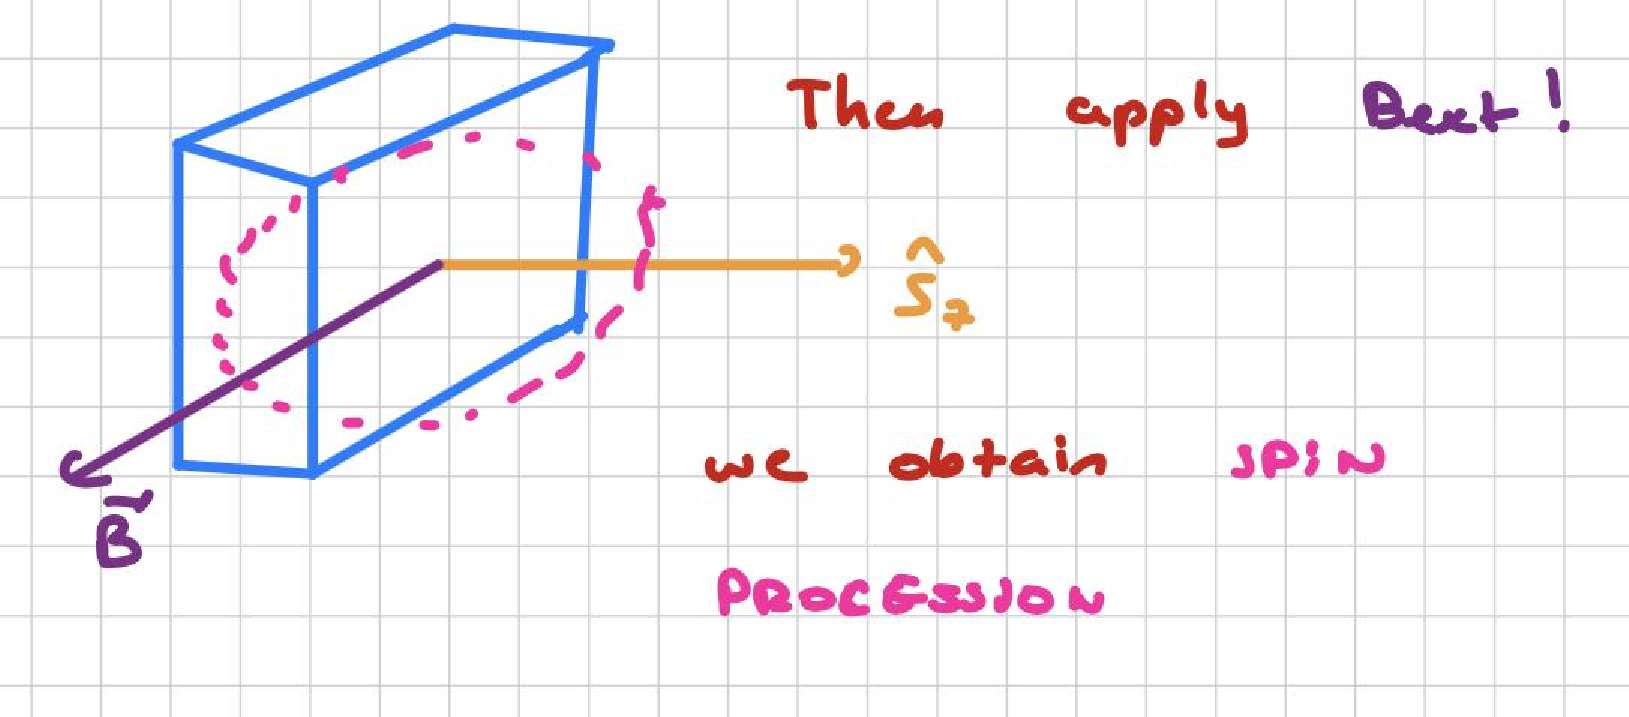
\includegraphics[width=0.8\textwidth]{images_in_pdf/3-/Grafico_17.pdf} 
\end{figure}

\subsubsection{Zeeman hamiltonian}

The Zeeman hamiltonian describes the interaction between the spin and the external magnetic field:
\begin{equation}\label{eqn:3-zeeman-hamiltonian}
\hat{H}_Z = -\vec{\mu}\cdot \vec{B}_{\mathrm{ext}} =
-g \mu_B \hat{\vec{S}}\cdot \vec{B}_{\mathrm{ext}},
\end{equation}

where $\vec{\mu}$ is the magnetic moment, $g$ is the carrier $g$-factor, $\mu_B$ is the Bohr magneton, and $\hat{\vec{S}}$ is the spin operator. In our case, since $\vec{B}_{\mathrm{ext}}$ is along $\hat{x}$,
\begin{equation}\label{eqn:3-zeeman-hamiltonian-2}
\hat{H}_Z =
-g \mu_B \hat{S}_x B_{\mathrm{ext}} =
-g \mu_B \frac{\hbar}{2} \hat{\sigma}_x B_{\mathrm{ext}}
\end{equation}

where we used the relation $\hat{S}_x = \frac{\hbar}{2} \hat{\sigma}_x$ between the spin operator and the Pauli matrix. Defining the \textbf{Larmor frequency} as $\omega_L = \frac{|g|\mu_B B_{\mathrm{ext}}}{\hbar}$, the hamiltonian becomes:
\begin{equation}\label{eqn:3-zeeman-hamiltonian-3}
    \hat{H}_Z = -\frac{1}{2} \hbar \omega_L \hat{\sigma}_x
\end{equation}

therefore its eigenstates are exactly the spin ones $\ket{\uparrow_x}$ and $\ket{\downarrow_x}$ with eigenvalues $\pm \frac{1}{2}\hbar \omega_L$.

\subsubsection{Spin dynamics}
As seen in the spin--injection process, the $\sigma^+$ pulse creates a neat population of spin--up electrons along the $z$-axis. Such state, $\ket{\uparrow_z}$, is a superposition of the two spin eigenstates along the $x$-axis, $\ket{\uparrow_x}$ and $\ket{\downarrow_x}$:
\begin{equation}\label{eqn:3-spin-superposition}
    \ket{\uparrow_z} = \frac{1}{\sqrt{2}}\left(\ket{\uparrow_x} + \ket{\downarrow_x}\right)
\end{equation}

Written like this, the time evolution of $\ket{\uparrow_z}$ under the Zeeman hamiltonian (Eqn.~\ref{eqn:3-zeeman-hamiltonian-3}) is straightforward to compute:
\begin{equation}\label{eqn:3-spin-superposition-time-evolution}
\ket{\uparrow_z(t)} = 
\frac{1}{\sqrt{2}}\left(\ket{\uparrow_x}e^{i\omega_L t/2} +
\ket{\downarrow_x}e^{-i\omega_L t/2}\right)
\end{equation} 

where the time--evolution operator $U(t) = e^{-i\hat{H}_Z t/\hbar}$ was used. Then, we can express the $x$--basis states in terms of the $z$--basis states, and perform a simple regroup of the terms:
\begin{equation}\label{eqn:3-x-basis-in-z-basis}
\begin{split}
\ket{\uparrow_z(t)} &=
\frac{1}{2}
\left[
\left(\ket{\uparrow_z}+\ket{\downarrow_z}\right)e^{i\omega_L t/2} +
\left(\ket{\uparrow_z}-\ket{\downarrow_z}\right)e^{-i\omega_L t/2}
\right]=\\[0.5ex]
&=\frac{1}{2}
\left[
\ket{\uparrow_z}\left(e^{i\omega_L t/2} + e^{-i\omega_L t/2}\right) +
\ket{\downarrow_z}\left(e^{i\omega_L t/2} - e^{-i\omega_L t/2}\right)
\right]
\end{split}
\end{equation}

here, we apply the Euler's formula:
\begin{equation}\label{eqn:3-euler-formula}
\begin{cases}
\cos\alpha = \frac{e^{i\alpha} + e^{-i\alpha}}{2}\\[0.5ex]
\sin\alpha = \frac{e^{i\alpha} - e^{-i\alpha}}{2i}
\end{cases}
\end{equation}

and we finally obtain:
\begin{equation}\label{eqn:3-spin-superposition-time-evolution-final}
\ket{\uparrow_z(t)} =
\ket{\uparrow_x}\cos\left(\frac{\omega_L t}{2}\right) + i\ket{\downarrow_x}\sin\left(\frac{\omega_L t}{2}\right)
\end{equation}

\calloutwarn{This means that the system oscillates coherently between spin--up and spin--down components.}


% questa immagine viene BOCCIATA! non ha senso
\begin{comment}
\begin{figure}[H]
    \centering            
    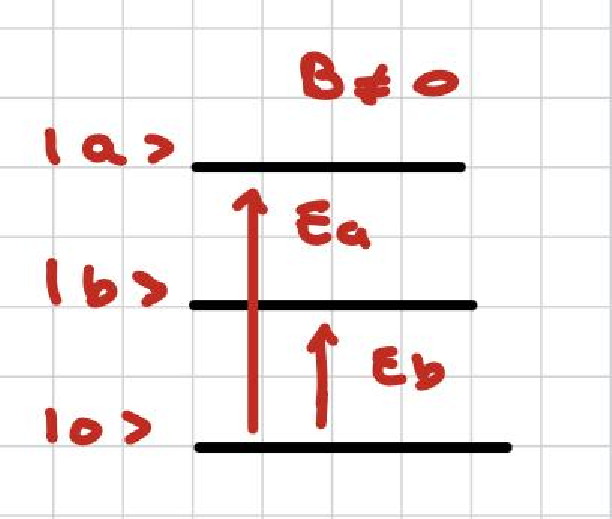
\includegraphics[width=0.4\textwidth]{images_in_pdf/3-/Grafico_18.pdf} 
\end{figure}
\end{comment}

When the luminescence emitted by the sample is measured, the circularly polarized components of the signal reflect this spin dynamics. 
For \textbf{zero magnetic field}, the emitted polarization typically shows a \textbf{monotonic decay}, as the non--equilibrium spin population relaxes toward thermal equilibrium with its characteristic \textbf{relaxation time}.
\begin{figure}[H]
    \centering
    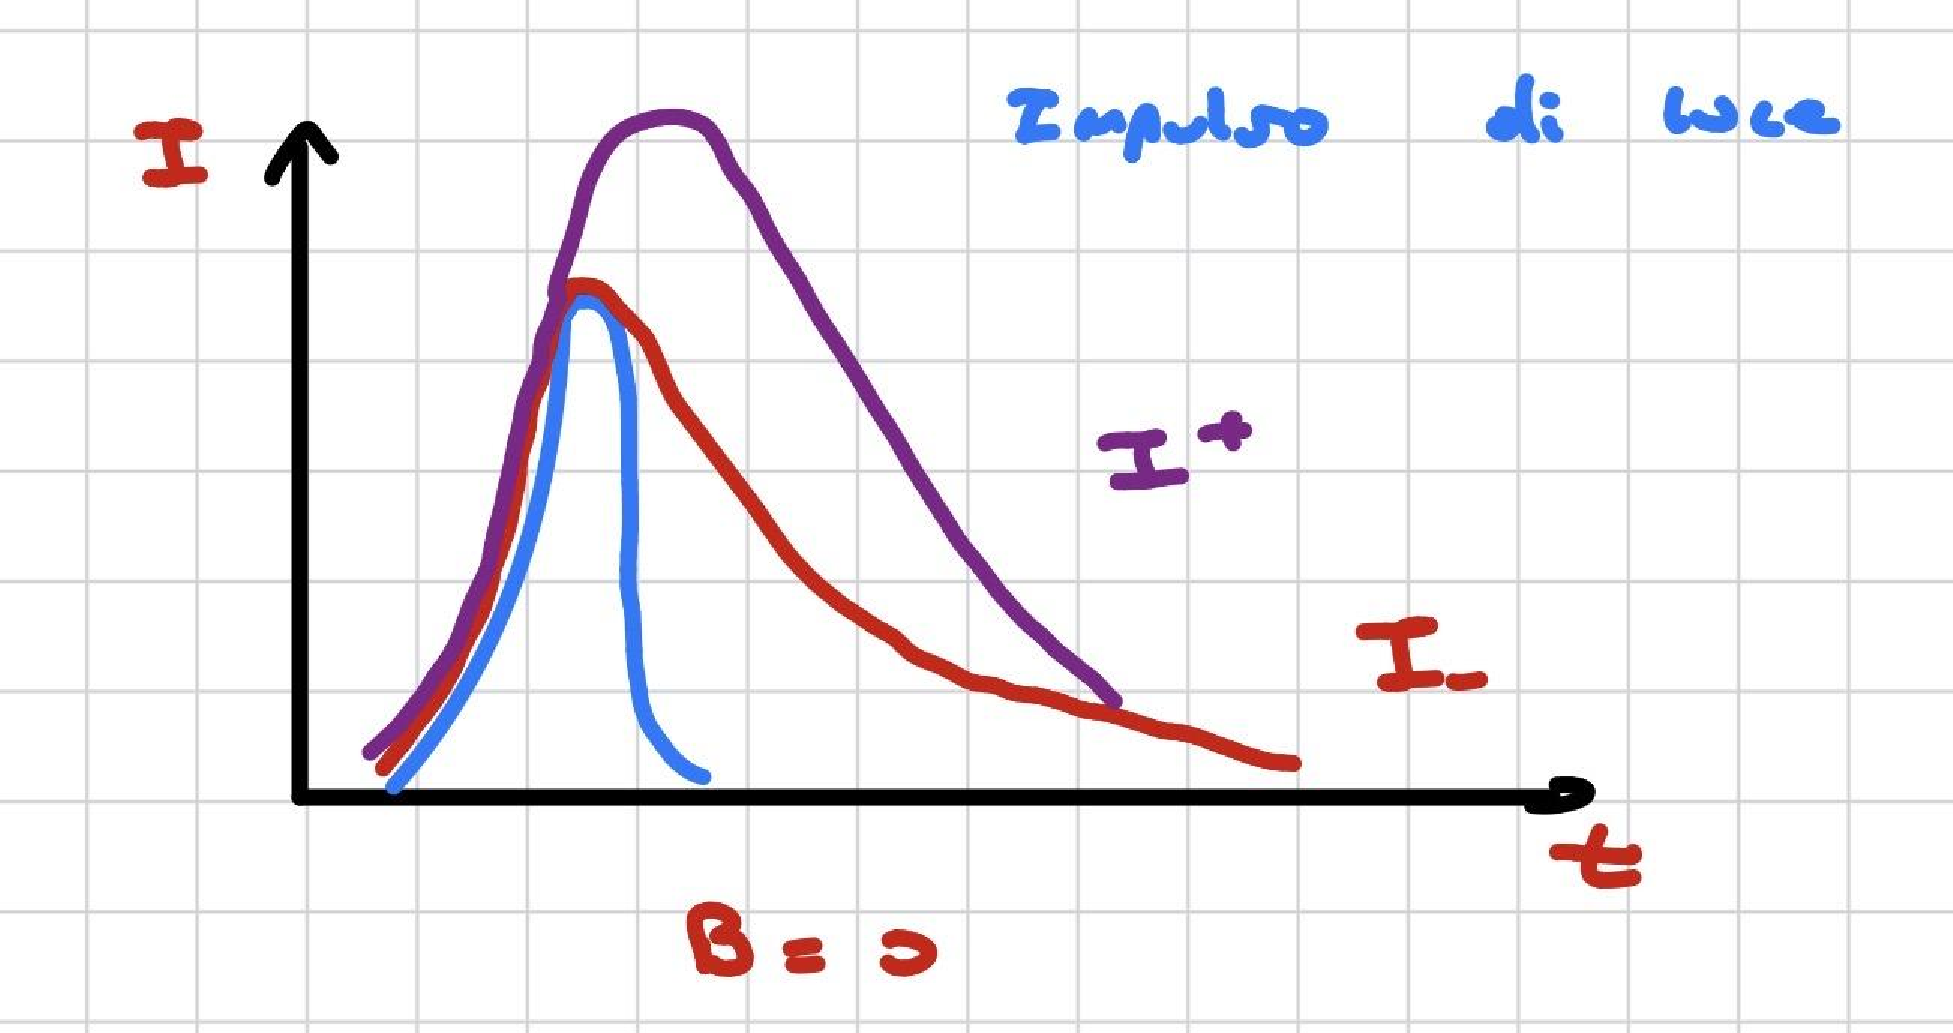
\includegraphics[width=0.6\linewidth]{images_in_pdf/3-/Grafico_19.pdf}
    \caption{$B=0$}
\end{figure}

In the figure, the blue curve represents the excitation pulse, while the other two curves correspond to the $\sigma^+$ and $\sigma^-$ components of the emitted luminescence. Their time dependence reflects an imbalance between the two circular polarizations, which gradually disappears because of spin relaxation.

\question{What happens when the magnetic field is turned on?}{Due to the Larmor precession, the two circular components now exhibit an oscillatory behavior, with alternating dominance in time.} 

\begin{figure}[H]
    \centering
    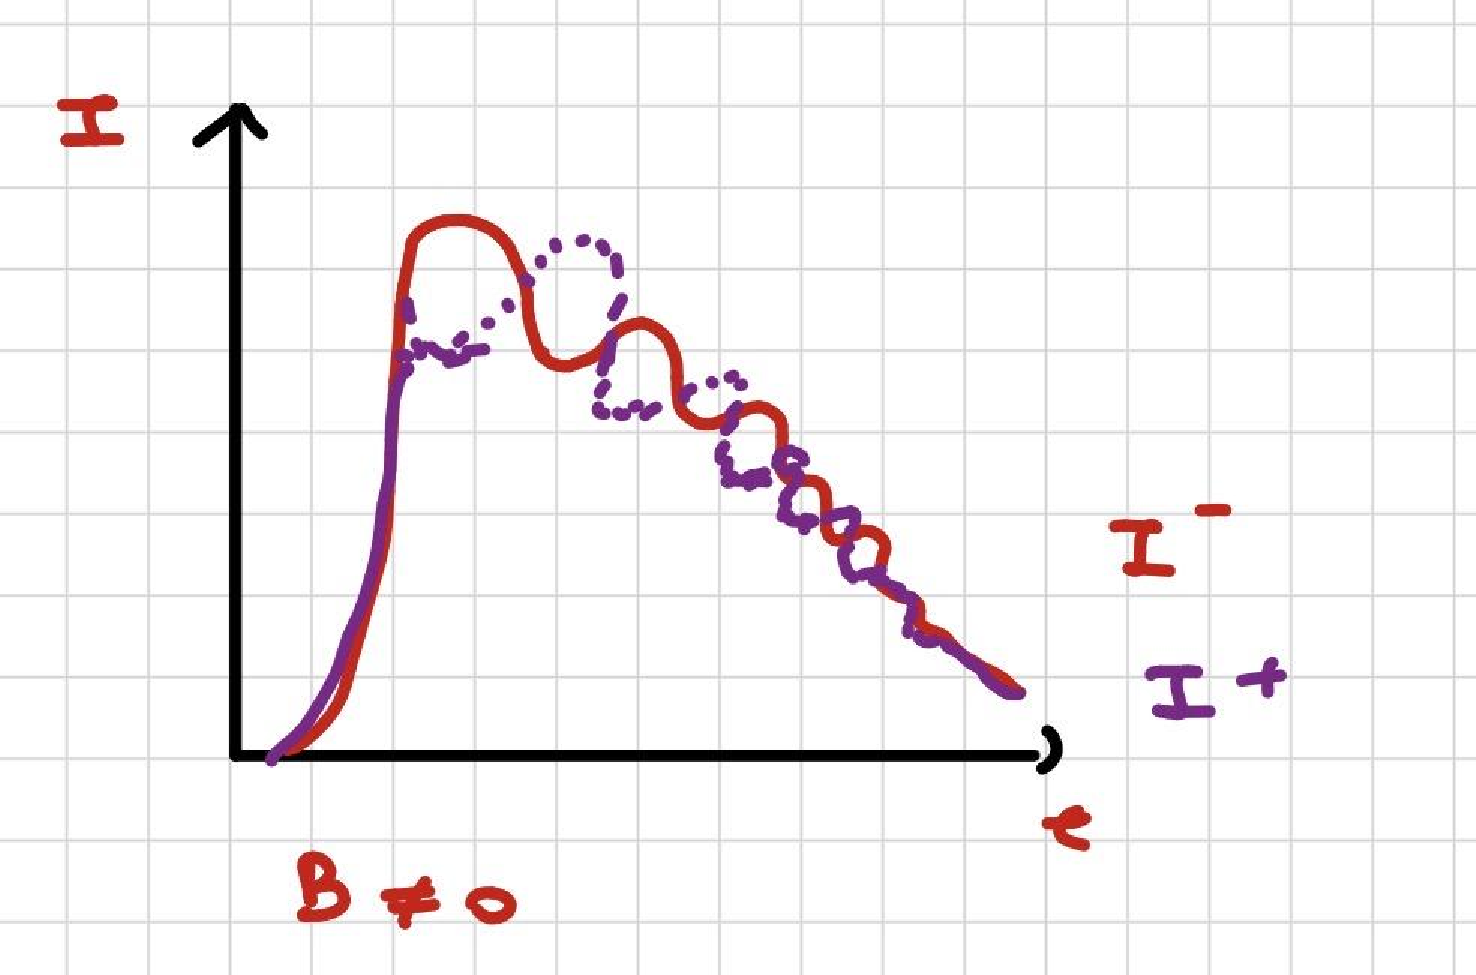
\includegraphics[width=0.6\linewidth]{images_in_pdf/3-/Grafico_20.pdf}
    \caption{$B \neq 0$}
\end{figure}

This relation is particularly useful since, measuring the oscillation frequency as a function of the magnetic field, one can \textbf{determine the $g$-factor} of the material. In the low-field regime, $\omega_L$ depends linearly on $B$, as expected from the Zeeman hamiltonian (Eqn.~\ref{eqn:3-zeeman-hamiltonian}).

At sufficiently high magnetic fields, deviations from linear behavior may appear because of additional contributions such as band non-parabolicity, orbital effects, anisotropy of the $g$-factor, or mixing with other states. These effects are not essential for the basic picture, but they can become relevant in precise experiments.

\section{Experiments with polarizers}\label{sec:exp-with-polarizers}

\subsection{Wire polarizers}\label{subsec:wire-polarizers}
In this subsection we discuss \textbf{wire polarizers}, which are optical components that transmit only the component of light polarized along a preferred direction, their \textbf{transmission axis}, while absorbing or suppressing the orthogonal component.

Suppose we have a wave propagating along the $z$-axis and consider a superposition of two linearly polarized waves:
\begin{equation*}
\begin{cases}
    \vec{E}_1(z,t) = (E_{0,x},0,0)\cos(kz-\omega t+\phi_1)\\
    \vec{E}_2(z,t) = (0,E_{0,y},0)\cos(kz-\omega t+\phi_2)
\end{cases}
\end{equation*}

where $\vec{E}_1$ is parallel to the $x$-direction and $\vec{E}_2$ is parallel to the $y$-direction. The total field amplitude can then be written as
\begin{equation}\label{eqn:4-field-amplitude}
    \vec{E}_0 = E_{0,x} \hat{x} + E_{0,y} \hat{y}
\end{equation}

If the light is incident on a polarizer whose optical axis is aligned with the $x$-direction, then the $x$-component is fully transmitted, while the $y$-component is blocked. In other terms:
\[
I_{\text{incoming}} \propto |\vec{E}_0|^2
\longrightarrow
I_{\text{transmitted}} \propto E_{0,x}^2
\]
More generally, if $\theta$ is the angle between the incoming polarization direction and the transmission axis, the transmitted intensity follows \textbf{Malus' law}:
\begin{equation}\label{eqn:malus-law}
I_{\text{transmitted}} = I_{\text{in}} \cos^2(\theta).
\end{equation}

Now suppose that, instead of a laser, we use a discharge lamp as the light source. In this case, the atoms in the lamp emit independently, so the outgoing light is an \textbf{incoherent mixture} of many polarization states with the same frequency. As a result, the light is not polarized overall. If such light passes through a polarizer, \textbf{the transmitted beam becomes linearly polarized along the transmission axis}, while the orthogonal component is removed.

\question{What happens if we send linearly polarized light, reduced to the single-photon level, through the polarizer? }{Suppose a detector is placed after the polarizer and we send $N$ photons:
\begin{itemize}
    \item If $\theta = 0^\circ$, all the photons pass through the polarizer.
    \item If $\theta = 90^\circ$, no photons are transmitted.
    \item For a generic angle $\theta$, the expected number of transmitted photons is $N\cos^2\theta$, while the remaining $N\sin^2\theta$ are not transmitted.
\end{itemize}}

If we observe the photons one by one, we find that each photon either passes through the polarizer or is absorbed. The outcome for each individual photon is probabilistic. Over many trials, the result of fraction of transmitted photons becomes more precise as $N$ increases.

\calloutinfo{For any single photon arriving at the polarizer, we cannot predict in advance whether it will be transmitted or not. We can only assign a probability to each outcome. This is a genuinely statistical result, and it has no direct classical analogue.}

One possible classical interpretation would be to assume the existence of \textbf{hidden variables:} in that picture, the polarization state would not be fully specified by the polarization vector $\vec{e}_{\theta,\phi}$ alone, but would also depend on an additional variable $\epsilon$ that could take the values $0$ or $1$, determining in advance whether the photon is transmitted or absorbed. We will return to this idea later. % TODO: inserire ref al paragrafo sulle disuguaglianze di Bell

\subsection{Beam splitters and random number generators}\label{subsec:4-BS-and-RNG}

Now consider a $50{:}50$ beam splitter (BS). In an ideal balanced beam splitter, each incoming photon has the same probability of being detected in output $D_1$ or in output $D_2$. The actual output event for each photon is random.
\hl{This property makes single-photon beam splitters a useful \emph{physical source of randomness}}. In practice, optical quantum random number generators are widely used because they exploit intrinsic quantum randomness rather than algorithmic pseudo-randomness.
Random numbers have many applications:
\begin{enumerate}
    \item \textbf{Cryptography}, where randomness is essential for secure keys and protocols;
    \item \textbf{Scientific simulations}, especially Monte Carlo methods for complex systems;
    \item \textbf{Lotteries and gambling}, where fairness requires unbiased random outcomes;e
    \item \textbf{Internet of Things and digital security}, where random keys are used to protect sensitive data.
\end{enumerate}
We can distinguish two main classes of random number generators:
\begin{itemize}
    \item \textbf{Software generators:} these are algorithms that take an initial value, called a seed, and produce a sequence of numbers by iteration. Since the sequence is deterministic and eventually periodic, these are usually called \emph{pseudo-random} number generators. They are inexpensive and useful in many numerical applications, but they are not truly random.
    \item \textbf{Generators based on physical processes:} these use a physical source of randomness.
    \begin{itemize}
        \item \textbf{Classical physical processes:} examples include coin tossing or dice rolling. In principle, classical dynamics is deterministic, but in practice the outcome is unpredictable because the initial conditions are not known with sufficient accuracy.
        \item \textbf{Quantum physical processes:} in this case randomness is intrinsic.
        \begin{enumerate}
            \item \textbf{Radioactive decay:} the decay time of a nucleus is fundamentally random, although this kind of source is not always practical or scalable for commercial devices.
            \item \textbf{Optical quantum processes:} these are already used in commercial quantum random number generators. For example, a single-photon source sent through a $50{:}50$ beam splitter produces a click in $D_1$ or $D_2$ with equal probability. One may assign the value $1$ when $D_1$ clicks and $0$ when $D_2$ clicks.
            \item \textbf{Vacuum fluctuations of the electromagnetic field:} these can also be exploited as a source of quantum randomness.
            \item \textbf{Photon-number fluctuations in light sources:} these are known as shot noise. Suppose to take a light source as a LED that goes on a matrix of detectors, each one receive a different amount of photons, as a random process. We measure the number of photons for each pixel and compute the average number. We impose to zero each pixel with number of photons below the average and reconstruct an image of fluctuations of photon numbers. Then we use apposite convertors to extract sequence of random numbers.
        \end{enumerate}
    \end{itemize}
\end{itemize}

\section{Cryptography}\label{sec:5-cryptography}

In modern cryptography, security is often based on practical computational constraints. A key example is \textbf{RSA encryption}, which relies on the difficulty of factoring large integers and is widely used in internet security. In RSA, the sender and receiver generate a \textbf{public key} and a \textbf{private key} respectively: the public key is shared openly and used to encrypt the message, while the private key is kept secret and used to decrypt it.

\subsection{Classical key distribution}\label{subsec:5-classical-key-distribution}
Let us consider two users, Alice and Bob, who want to communicate securely in the presence of a third party, Eve, who tries to read the message.

Bob performs the following steps:
\begin{itemize}
    \item Choose two large prime numbers, $p$ and $q$;
    \item Compute $n = p q$ and publish it on the public channel;
    \item Compute $\varphi(n) = (p-1)(q-1)$;
    \item Choose an integer $e$ such that $\gcd(e,\varphi(n))=1$, and publish it on the public channel;
    \item Compute the private exponent $d$ as the modular inverse of $e$ modulo $\varphi(n)$, namely
    \[
    d \equiv e^{-1} \pmod{\varphi(n)}.
    \]
\end{itemize}
Here $\gcd$ denotes the greatest common divisor, i.e. the largest positive integer dividing both numbers. The notation $x \equiv y \pmod{n}$ means that $x-y$ is an integer multiple of $n$.

Alice then does the following:
\begin{itemize}
    \item Choose the message $M$;
    \item Compute the encrypted message
    \[
    C \equiv M^e \pmod{n};
    \]
    \item Send $C$ to Bob through the public channel.
\end{itemize}
Bob decrypts the message by computing
\[
M \equiv C^d \pmod{n}.
\]
The security of RSA relies on the fact that Eve knows $n$ and $e$, but in order to find $d$ she would need to factorize $n$ into $p$ and $q$. For \textbf{sufficiently large} $n$ this is \textbf{computationally infeasible} with classical algorithms. However, quantum computers would be able to solve the factoring problem efficiently using Shor's algorithm.

\subsection{Quantum key distribution}\label{subsec:quantum-key-distribution}
Suppose that a beam of light is sent onto a \textbf{polarized beam splitter}. Three cases are relevant:
\begin{itemize}
    \item \textbf{State} $\ket{H}$: the light is horizontally polarized and is transmitted to detector $D_1$.
    \item \textbf{State} $\ket{V}$: the light is vertically polarized and is reflected to detector $D_2$.
    \item \textbf{State} $\ket{\theta}$: the light is prepared in a superposition of horizontal and vertical polarization, so both detectors may receive a signal with different probabilities.
\end{itemize}
\begin{figure}[H]
    \centering
    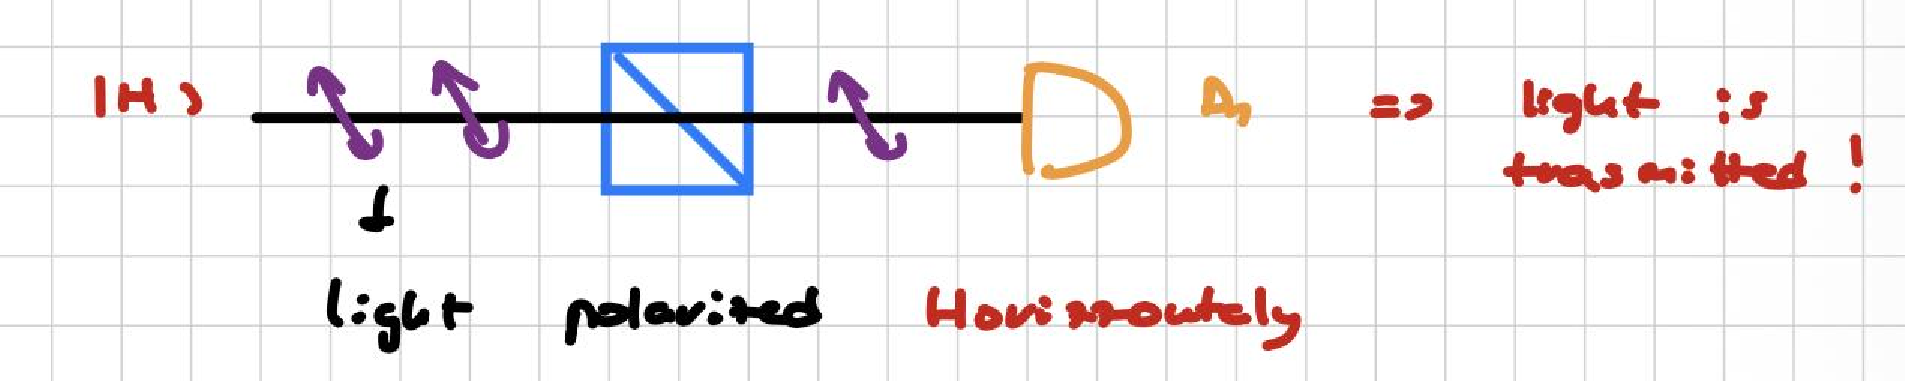
\includegraphics[width=0.9\linewidth]{images_in_pdf/5-/Grafico_21.pdf}
\end{figure}
\begin{figure}[H]
    \centering
    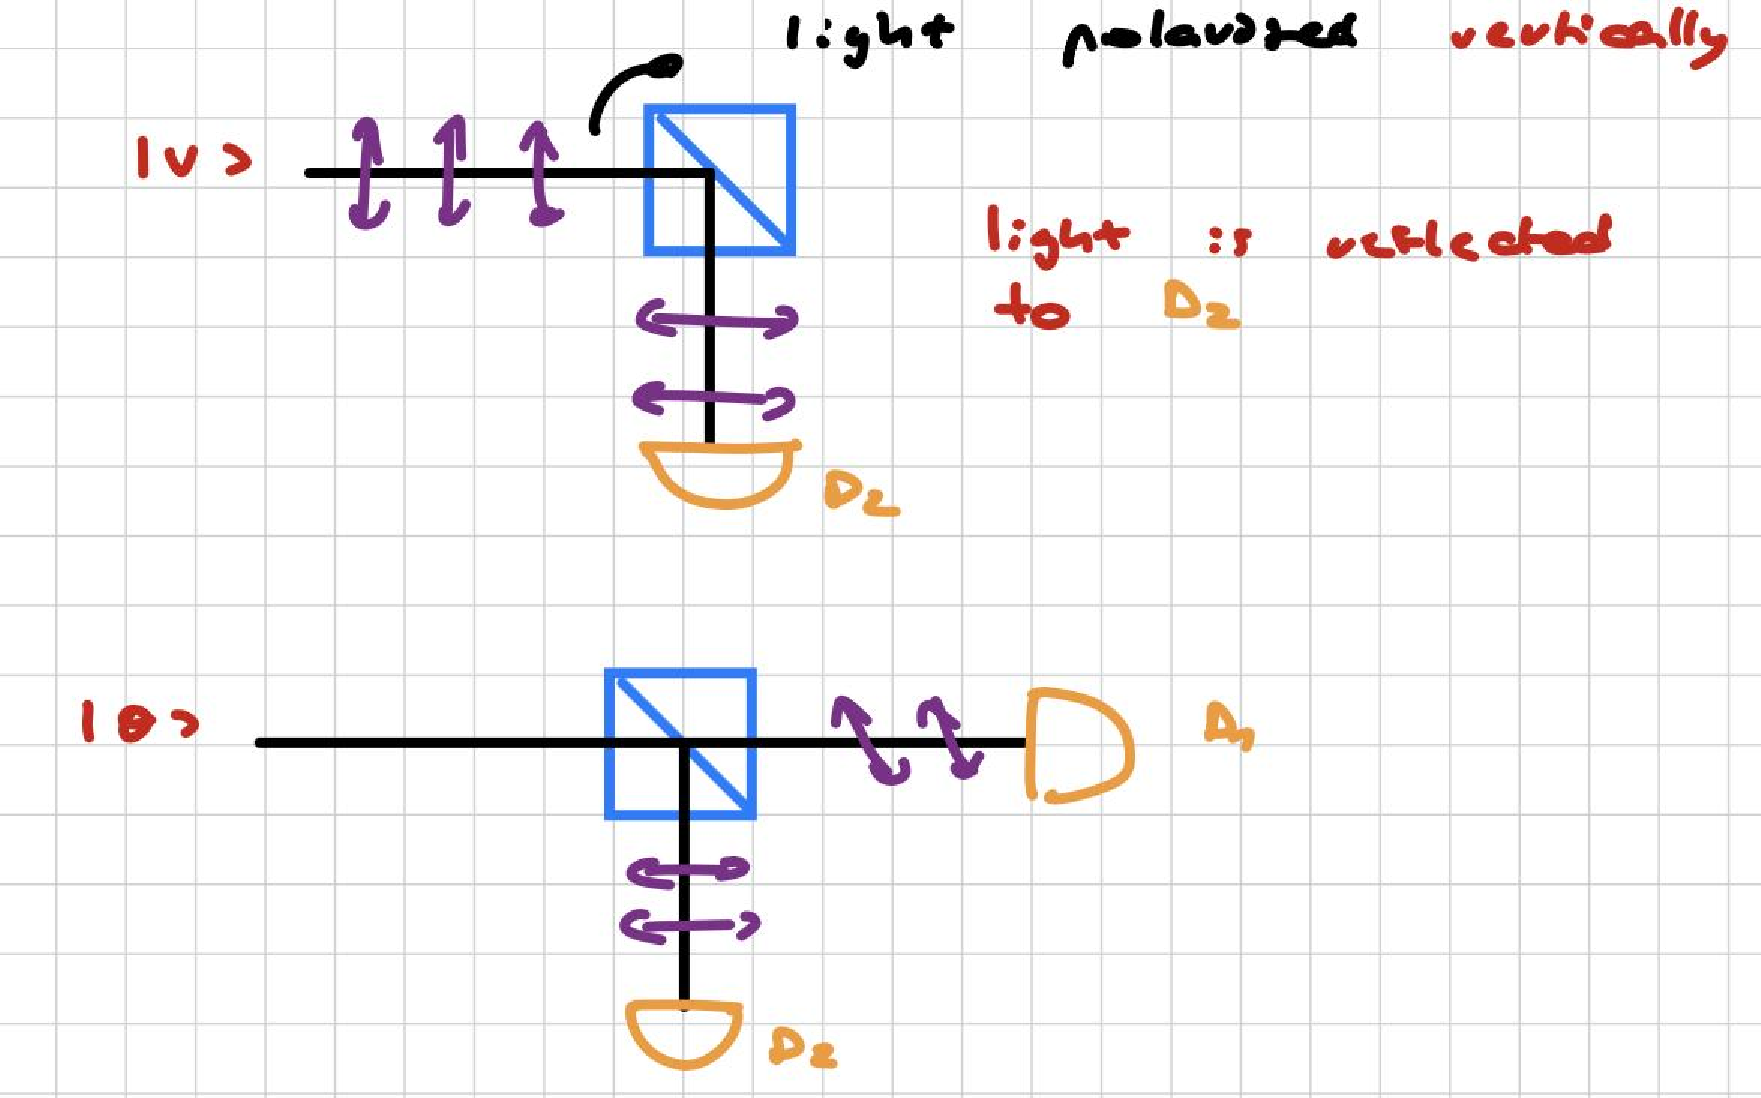
\includegraphics[width=0.8\linewidth]{images_in_pdf/5-/Grafico_22.pdf}
\end{figure}

For a generic linearly polarized state,
\[
\ket{\theta} = \cos(\theta)\ket{H} + \sin(\theta)\ket{V},
\]
the probabilities of obtaining the two outcomes are
\[
P_H = |\braket{H|\theta}|^2 = \cos^2(\theta),
\qquad
P_V = |\braket{V|\theta}|^2 = \sin^2(\theta).
\]
For a diagonal state, we define
\[
\ket{D_+} = \frac{1}{\sqrt{2}}\left(\ket{H}+\ket{V}\right),
\qquad
\ket{D_-} = \frac{1}{\sqrt{2}}\left(\ket{H}-\ket{V}\right).
\]
These states are orthogonal and form another basis of the polarization Hilbert space. In this way, polarized photons can be used to encode one bit of information.

The key idea is that Alice and Bob want to communicate, while Eve wants to intercept the message. If Eve measures a photon in the same basis used by Alice, she can reproduce the state correctly. However, if she measures in the wrong basis, the state is disturbed. When she re--sends the photon to Bob, her intervention becomes detectable. Thus, \hl{the measurement process modifies the quantum state itself}, revealing Eve's presence.

\question{Why not make copies of the original state and measure the copies instead?}{This is impossible because of the \textbf{no-cloning theorem}.}

\textbf{Proof idea:} suppose a ``quantum Xerox machine'' exists, i.e. a device that takes an unknown state $\ket{\psi}$ and a blank state $\ket{X}$ and produces two identical copies:
\[
\ket{\psi}\ket{X} \longrightarrow \ket{\psi}\ket{\psi}.
\]
Assume that the machine works for the basis states $\ket{H}$ and $\ket{V}$:
\[
\ket{H}\ket{X} \longrightarrow \ket{H}\ket{H},
\qquad
\ket{V}\ket{X} \longrightarrow \ket{V}\ket{V}.
\]
Because quantum evolution is linear, it should also work for the superposition
\[
\ket{D_+} = \frac{1}{\sqrt{2}}\left(\ket{H}+\ket{V}\right).
\]
Linearity would imply
\[
\ket{D_+}\ket{X} \longrightarrow \frac{1}{\sqrt{2}}\left(\ket{H}\ket{H}+\ket{V}\ket{V}\right),
\]
whereas perfect cloning would require
\[
\ket{D_+}\ket{X} \longrightarrow \ket{D_+}\ket{D_+}
= \frac{1}{2}\left(\ket{H}\ket{H}+\ket{H}\ket{V}+\ket{V}\ket{H}+\ket{V}\ket{V}\right).
\]
These two results are different, so a universal cloning machine cannot exist.

\callout{No cloning theorem - Alternative proof}{%
\begin{proof}
Suppose there exists a unitary operator $U=U^\dagger$ such that:
\begin{equation*}
\begin{cases}
    U\ket{\psi}\otimes\ket{\phi} = \ket{\psi}\otimes\ket{\psi}\\
    U\ket{\varphi}\otimes\ket{\phi} = \ket{\varphi}\otimes\ket{\psi}
\end{cases}
,\quad \forall \ket{\psi}, \ket{\varphi}, \ket{\phi} \in \mathcal{H},
\end{equation*}
where the states are normalized. Since unitary operators preserve inner products, it should hold that:
\begin{equation*}
    \left(\bra{\psi}\otimes\bra{\phi}\right)
    \left(\ket{\varphi}\otimes\ket{\phi}\right) =
    \left(\bra{\psi}\otimes\bra{\psi}\right)
    \left(\ket{\varphi}\otimes\ket{\varphi}\right)
\end{equation*}

following $\braket{\phi|\phi} = 1$:
\begin{equation*}
    \braket{\psi|\varphi} = \braket{\psi|\varphi}\braket{\psi|\varphi}
\end{equation*}

and this is only possible if the inner product $\braket{\psi|\varphi}$ is either $0$ or $1$. In other words, the states $\ket{\psi}$ and $\ket{\varphi}$ must be either \textbf{orthogonal} or \textbf{identical} up to a phase, which contradicts the assumption that the cloning operator works for all states.
\end{proof}
}

For this reason, Alice can send Bob a string of bits encoded in single photons prepared in one of the polarization states $\ket{H}$, $\ket{V}$, $\ket{D_+}$, or $\ket{D_-}$, while choosing the basis at random. Eve cannot copy the photons without introducing errors. By comparing a subset of their bits, Alice and Bob can detect whether the channel has been intercepted.

\subsection{BB84: first Quantum Cryptography Protocol}\label{subsec:BB84}
The BB84 protocol is a quantum key distribution scheme. It does not directly encrypt the message; rather, it allows Alice and Bob to \hl{generate a shared secret key}, which can later be used in a one-time pad.

The encrypted message is obtained by adding, modulo $2$, the message bits and a secret random key of the same length. For example,
\[
0 \oplus 0 = 0,\qquad 1 \oplus 0 = 1,\qquad 0 \oplus 1 = 1,\qquad 1 \oplus 1 = 0.
\]
Bob can decrypt the message using the same key.

The two bases used in BB84 are:
\begin{itemize}
    \item \textbf{Rectilinear basis} $+$: $\ket{H} \mapsto 0$ and $\ket{V} \mapsto 1$;
    \item \textbf{Diagonal basis} $\times$: $\ket{D_+} \mapsto 0$ and $\ket{D_-} \mapsto 1$.
\end{itemize}
The experimental setup consists of:
\begin{itemize}
    \item[--] a single-photon source;
    \item[--] polarization preparation optics, such as polarizers and wave plates;
    \item[--] a polarizing beam splitter, which separates the two orthogonal polarizations into transmitted and reflected outputs;
    \item[--] two single-photon detectors.
\end{itemize}
The protocol proceeds as follows:
\begin{enumerate}
    \item Alice randomly chooses a basis and a bit value, then sends the corresponding photon state.
    \item Bob randomly chooses a measurement basis and records the detector outcome.
    \item After the transmission, Alice and Bob publicly compare their basis choices and keep only the events where the bases match. 
\end{enumerate}
The possible configurations are summarized in Table~\ref{tab:bb84}.

\begin{table}[H]
\label{tab:bb84}
\centering
\renewcommand{\arraystretch}{1.3}
\begin{tabular}{|c|c|c||c|c|c||c|}
\hline
\multicolumn{3}{|c||}{\textbf{Alice (A)}} & 
\multicolumn{3}{c||}{\textbf{Bob (B)}} & 
\textbf{Basis} \\
\textbf{Basis} & \textbf{State} & \textbf{Bit} &
\textbf{Basis} & $D_1$ & $D_2$ &
\textbf{Match} \\
\hline
$+$ & $\ket{H}$ & 0 & $+$ & 100\% & 0\% & Yes \\
$+$ & $\ket{V}$ & 1 & $+$ & 0\% & 100\% & Yes \\
$\times$ & $\ket{D_+}$ & 0 & $+$ & 50\% & 50\% & No \\
$\times$ & $\ket{D_-}$ & 1 & $+$ & 50\% & 50\% & No \\
$+$ & $\ket{H}$ & 0 & $\times$ & 50\% & 50\% & No \\
$+$ & $\ket{V}$ & 1 & $\times$ & 50\% & 50\% & No \\
$\times$ & $\ket{D_+}$ & 0 & $\times$ & 100\% & 0\% & Yes \\
$\times$ & $\ket{D_-}$ & 1 & $\times$ & 0\% & 100\% & Yes \\
\hline
\end{tabular}
\caption{BB84 quantum key distribution protocol: polarization states, measurement bases, and basis matching.}
\end{table}


The measurement operators associated with the two bases can be written as
\begin{equation}\label{5-measurement-operators}
\hat{M}_{+} = \ket{H}\bra{H} - \ket{V}\bra{V},
\qquad
\hat{M}_{\times} = \ket{D_+}\bra{D_+} - \ket{D_-}\bra{D_-}.
\end{equation}

So that, for example, the action of $\hat{M}_+$ on the $+$ and $\times$ basis states is:
\begin{equation}\label{5-measurement-operators-action}
\begin{cases}
\hat{M_+} \ket{H} = 1 \cdot \ket{H}\\
\hat{M_+} \ket{V} = -1 \cdot \ket{V}
\end{cases}
\hspace{1cm}
\begin{cases}
\hat{M_+} \ket{D_+} = 
\tfrac{1}{\sqrt{2}} \left(\ket{H} -\ket{V}\right) \equiv \ket{D_-}\\ 
\hat{M_+} \ket{D_-} = 
\tfrac{1}{\sqrt{2}} \left(\ket{H} +\ket{V}\right) \equiv \ket{D_+}
\end{cases}
\end{equation}

While $\ket{H}$ and $\ket{V}$ are its eigenstates with eigenvalues $1$ and $-1$ respectively, when it acts on $\ket{D_{\pm}}$ a superposition of the states $\ket{H}$ and $\ket{V}$ is returned.

\calloutinfo{If Alice and Bob choose the same basis, the bit value is preserved. If they choose different bases, the measurement outcome is random.}

\question{What happens if Eve intercepts the photon?}{
Suppose Alice uses the $+$ basis:
\begin{itemize}
    \item if Eve and Bob both choose the $+$ basis, Eve reads the right bit and re--sends the correct photon and Bob reads the correct bit;
    \item if Eve chooses the $+$ basis but Bob chooses the $\times$ basis, Bob obtains a random result, the bit would be discarded anyway;
    \item if Eve chooses the $\times$ basis and Bob chooses the $+$ basis, Bob again obtains a random result;
    \item if Eve and Bob both choose the $\times$ basis, Eve has already disturbed the state and Bob may obtain the wrong result after basis reconciliation.
\end{itemize}
The same reasoning applies if Alice initially chooses the $\times$ basis.
}

Alice and Bob do not keep all transmitted bits. Instead, they generate a longer raw key, publicly compare a subset of the bits, and discard the mismatched ones. For example, if they need a final key of 1064 bits, they may transmit a longer string, reveal a sample of check bits, and keep the rest.

If Alice reveals the first bit as $(+,0)$ then an intercept--resend attack by Eve has the following structure:
\begin{equation}\label{5-eve-attack}
A(+,0) \implies
\begin{cases}
E[P=50\%, +,0] \implies B[P=100\%, +,0] \implies P_{\text{tot}} = 50\% \\
E[P=50\%, \times, (0,1)] \implies
\begin{cases}
B[P=50\%, +,0] \implies P_{\text{tot}} = 25\% \\
B[P=50\%, +,1] \implies P_{\text{tot}} = 25\%
\end{cases}
\end{cases}
\end{equation}

\hl{In $3/4$ of the cases, Eve can get away with the single--bit attack}, which means that the detection probability is
\[
P_{\text{detected}} = 25\%,
\qquad
P_{\text{undetected}} = 75\%.
\]
If Eve attacks $n$ independent bits, the probability of remaining undetected is
\[
P_{\text{undetected}} = \left(\frac{3}{4}\right)^n,
\]
so the \textbf{probability of detecting} Eve is
\[
P_{\text{detected}} = 1 - \left(\frac{3}{4}\right)^n.
\]
For sufficiently large $n$, this probability becomes very close to $1$.

Eve's not the only source of error, others are:
\begin{itemize}
    \item photon loss during transmission;
    \item inefficient coupling to the detector;
    \item detector inefficiency;
    \item birefringent materials, which may rotate or distort the polarization during propagation;
    \item detector noise.
\end{itemize}

All these will increase the number of discarded bits and a overall reduction of the data transfer rate. We need to apply \textbf{error correction} by a parity check on a subset of bits;

\question{Which is the right number of bits?}{%
This is given by \textbf{Shannon's Noisy Channel Coding Theorem:} 
\begin{equation}\label{5-shannon}
N_{needed} = N \cdot [-\epsilon\cdot log_2(\epsilon)-(1-\epsilon)\cdot log_2(1-\epsilon)]
\end{equation}
where $N =$ total number of bits and $\epsilon = $ error propagation, if 
\[\epsilon \to + \infty \implies N_{needed} \to +\infty\] 
which means that we need to make sure that:
\begin{equation}\label{5-shanon-condition}
    \epsilon << \epsilon_{Eve}
\end{equation}
}

We also need an \textbf{authentication process} which consists in an exchange of few bits between Alice and Bob at the beginning according to a key, in this way Alice is sure to be communicating with Bob.

\chapter{Light statistics and photodetection}\label{chap:6-stat-props-of-light}

\section{Statistical properties of light}\label{sec:stat-props-of-light}
Classical models describe light as a continuous train of electromagnetic waves, but this is only an approximation, since real light is emitted by atoms, with a \textbf{finite lifetime}. However, this lifetime is typically much shorter than the detector integration time $\tau_D$, which means that \textbf{individual emission bursts cannot be resolved}. As a consequence, one observes a well-defined average intensity that fluctuates on timescales longer than $\tau_D$. 

We can model classical light sources as a large number of atoms emitting independently. In a gas, atoms move and produce frequency shifts, while collisions interrupt the emission process and randomize the phase, leading to phase fluctuations.

Observe that:
\begin{itemize}
    \item A light source has a finite spectral width, meaning that its frequency is not perfectly constant. It also exhibits \textbf{intensity noise}, which implies that the amplitude of the light changes in time due to fluctuations in the number of emitting atoms and to random phase jumps in the field emitted by individual atoms. These features allow us to distinguish between classical and quantum light sources;
    
    \item Studying line-shapes with spectroscopy also provides information about the energy levels of the emitting system;
    
    \item Measuring the statistical properties of light gives access to temporal noise traces, which are relevant in quantum optics, as well as to coherence and correlation functions.
\end{itemize}

If we recall the Mach-Zehnder interferometer (Fig.~\ref{1-mach-zehnder}), the interference fringes are determined by the phase difference between the beams propagating along the two optical paths. All the discussion made before assumes a stable source frequency.
\calloutwarn{If the source has a finite spectral width $\Delta\omega$, the fringes are washed out because the contributions associated with different frequencies no longer interfere with full visibility, \textbf{bright fringes} with $\omega_1$ right \textbf{overlap with dark fringes} with $\omega_2$.}

\subsection{Coherence}

We can define \textbf{coherence} as the degree of correlation of the field, and it can be spatial or temporal. In the present discussion we are interested in temporal fluctuations, which are quantified by the \textbf{coherence time} $\tau_c$, defined as the \hl{duration over which the phase of the wave train remains correlated}. In the same way, we can define the \textbf{coherence length} as
\[
L_c = c\,\tau_c.
\]

\calloutinfo{In a Mach-Zehnder interferometer, interference fringes can be observed only when the optical path difference is smaller than the coherence length $L_c$.}

\subsection{Chaotic light sources}\label{subsec:6-chaotic-light-sources}

Suppose that:
\begin{itemize}
    \item The light source is a \textbf{gas discharge lamp}, where the atoms are excited and emit radiation. The emission is determined by the spread in atomic velocities (\emph{Doppler broadening}) and by random emission events. Such a source is called a \textbf{chaotic light source}, like thermal cavities and filament lamps.
    
     \item We assume that \textbf{collision broadening dominates}, which causes elastic phase interruptions. Atoms emit trains of electromagnetic waves, but \hl{collisions shift the energy levels and interrupt the radiation emission}. After a collision, emission resumes with the same characteristics as before, but the phase is now unrelated to the previous one. 
     Let us assume that the collision time is short, so that we can neglect the radiation emitted during the collision itself.
     
    \item Suppose to assume that the \textbf{polarization is fixed} and we can focus light in order to obtain a well defined collimated beam far away from the source. 
 \end{itemize}

The total amplitude of the electric field, sum of the emission of each atom independent one to another, would be:
\begin{equation}\label{eqn:6-total-field}
\begin{split}
E_{\text{tot}}(t) &= \sum_{i=1}^{N} E_i(t) = \\[0.5ex]
&= E_0 e^{-i\omega_0 t}\sum_{i=1}^{N} e^{i\phi_i(t)} = \\[0.5ex]
&= E_0 e^{-i\omega_0 t}\, a(t)\, e^{i\phi(t)}
\end{split}
\end{equation}

where $E_0$ and $\omega_0$ are constants, while $\phi(t)$ changes over time after each collision. Here the phase angles $\phi_1,\ldots,\phi_N$ fluctuate randomly, so the corresponding phasors can be viewed as unit vectors oriented in random directions. In phase space, this can be imagined as a random-walk process.

\hl{The total field therefore consists of a wave at frequency $\omega_0$ with \textbf{random amplitude} $a(t)$ and \textbf{random phase}}.
Notice that at optical frequencies, $f\approx 10^{15}\,\text{Hz}$, the electric field varies extremely rapidly in time, so its instantaneous value is not practical to measure. It is better to perform a time average.

We now introduce the \textbf{Poynting vector} for a wave propagating along the generic direction $\hat{k}$:
\begin{equation}\label{eqn:6-generic-em-wave}
\begin{cases}
    \vec{E} = \vec{E}_0 \cos(\vec{k}\cdot\vec{r}-\omega t)\\[0.5ex]
    \vec{B} = \vec{B}_0 \cos(\vec{k}\cdot\vec{r}-\omega t)
\end{cases}
\end{equation}
\begin{equation}\label{eqn:6-poynting-vector}
\begin{split}
    \vec{S}&=\frac{1}{\mu_0}\,\vec{E}\times\vec{B}=\\[0.5ex]
    &=\varepsilon_0 c^2\,\vec{E}\times\vec{B}=
    \varepsilon_0 c^2\,\vec{E}_0\times\vec{B}_0\,
    \cos^2(\vec{k}\cdot\vec{r}-\omega t)=\\[0.5ex]
    &=\varepsilon_0 c^2 E_0 B_0 \cos^2(\vec{k}\cdot\vec{r}-\omega t) \hat{k}
\end{split}
\end{equation}

If we take the cycle average over a period $T$ of the Equation~\ref{eqn:6-poynting-vector}:
\begin{equation}\label{eqn:6-generic-em-wave-intensity}
    I\coloneqq\langle \vec{S}\rangle_T
    =\frac{1}{2}\varepsilon_0 c^2 E_0B_0
    =\frac{1}{2}\varepsilon_0 c E_0^2
\end{equation}

since for a plane wave $B_0=E_0/c$. 

In our case, having $E_\text{tot}(t)$ given by the Eq.~\ref{eqn:6-total-field}:
\begin{equation}\label{eqn:6-chaotic-light-intensity}
    I=\varepsilon_0 c\,\langle \vec{E}^{\,2}\rangle_T
    =\varepsilon_0 c\cdot \frac{1}{2}E_0^2 a^2(t)
\end{equation}

where $a(t)$ is the modulation amplitude.

The spectral width $\Delta\omega$ is determined by the average collision time according to the energy-time uncertainty principle:
\begin{equation}\label{eqn:6-energy-time-uncertainty}
\Delta E \Delta t \geq \hbar
\implies
\frac{\Delta E}{\hbar} \geq \frac{1}{\Delta t} \coloneqq
\frac{1}{\tau} = \frac{\Delta\omega}{2\pi}
\end{equation}

\begin{figure}[H]
    \centering
    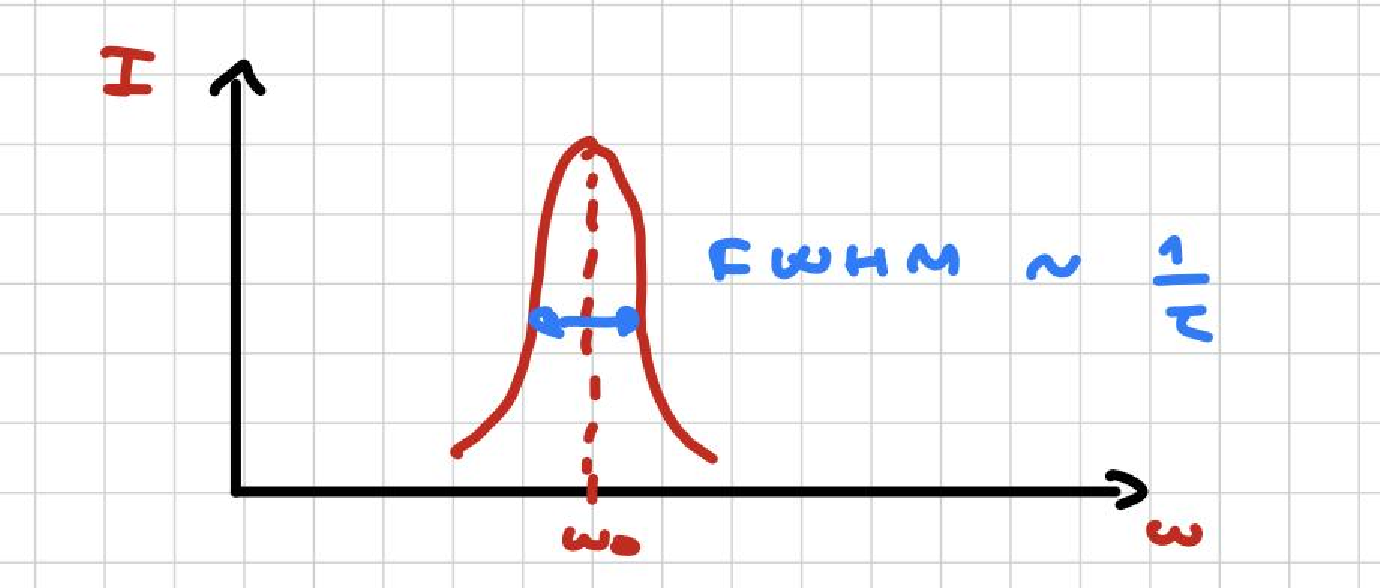
\includegraphics[width=0.8\linewidth]{images_in_pdf/6-/Grafico_23.pdf}
\end{figure}

The collision time $\tau_{\text{collision}}$ is typically shorter than the radiative lifetime, so the spectral width is mainly determined by collisions:
\[
\Delta\omega \approx \frac{1}{\tau_{\text{collision}}}
\]

Physically, this can be understood by noting that each atom emits a coherent wave only for a finite time between two successive collisions. Each collision interrupts the emission and randomizes the phase, so the emitted field can be seen as a sequence of short wave packets. According to Fourier analysis, a shorter emission time in the time domain corresponds to a broader distribution in frequency, which explains the increase in spectral width.

The coherence time is therefore limited by the same mechanism and is inversely related to the spectral width:
\[
\tau_c \approx \frac{1}{\Delta\omega}
\]

From a physical point of view, \hl{the coherence time represents the timescale over which the phase of the electromagnetic field remains correlated, i.e., how long the field \mbox{\say{remembers}} its phase}. Frequent collisions lead to rapid phase randomization and thus to a short coherence time.

In general, the \textbf{coherence time is determined by the spectral width and we can classify light with it}:
\begin{itemize}
    \item \textbf{Perfect monochromatic} source: $\Delta\omega=0$, which implies perfect phase correlation (ideal case, e.g. lasers), and therefore $\tau_c\to +\infty$.
    \item Thermal sources or \textbf{white light}: $\Delta\omega$ is broad, implying rapid phase fluctuations and therefore a very short coherence time.
\end{itemize}

\calloutinfo{For a \textbf{Doppler-broadened} source the frequencies of the emitted radiation are distributed according to a Gaussian function. This originates from the thermal motion of atoms: each atom moves with a different velocity and, due to the Doppler effect, emits radiation at a slightly shifted frequency. Since the \textbf{atomic velocities follow a Maxwell-Boltzmann distribution}, the resulting frequency distribution is Gaussian.}

\begin{figure}[H]
    \centering
    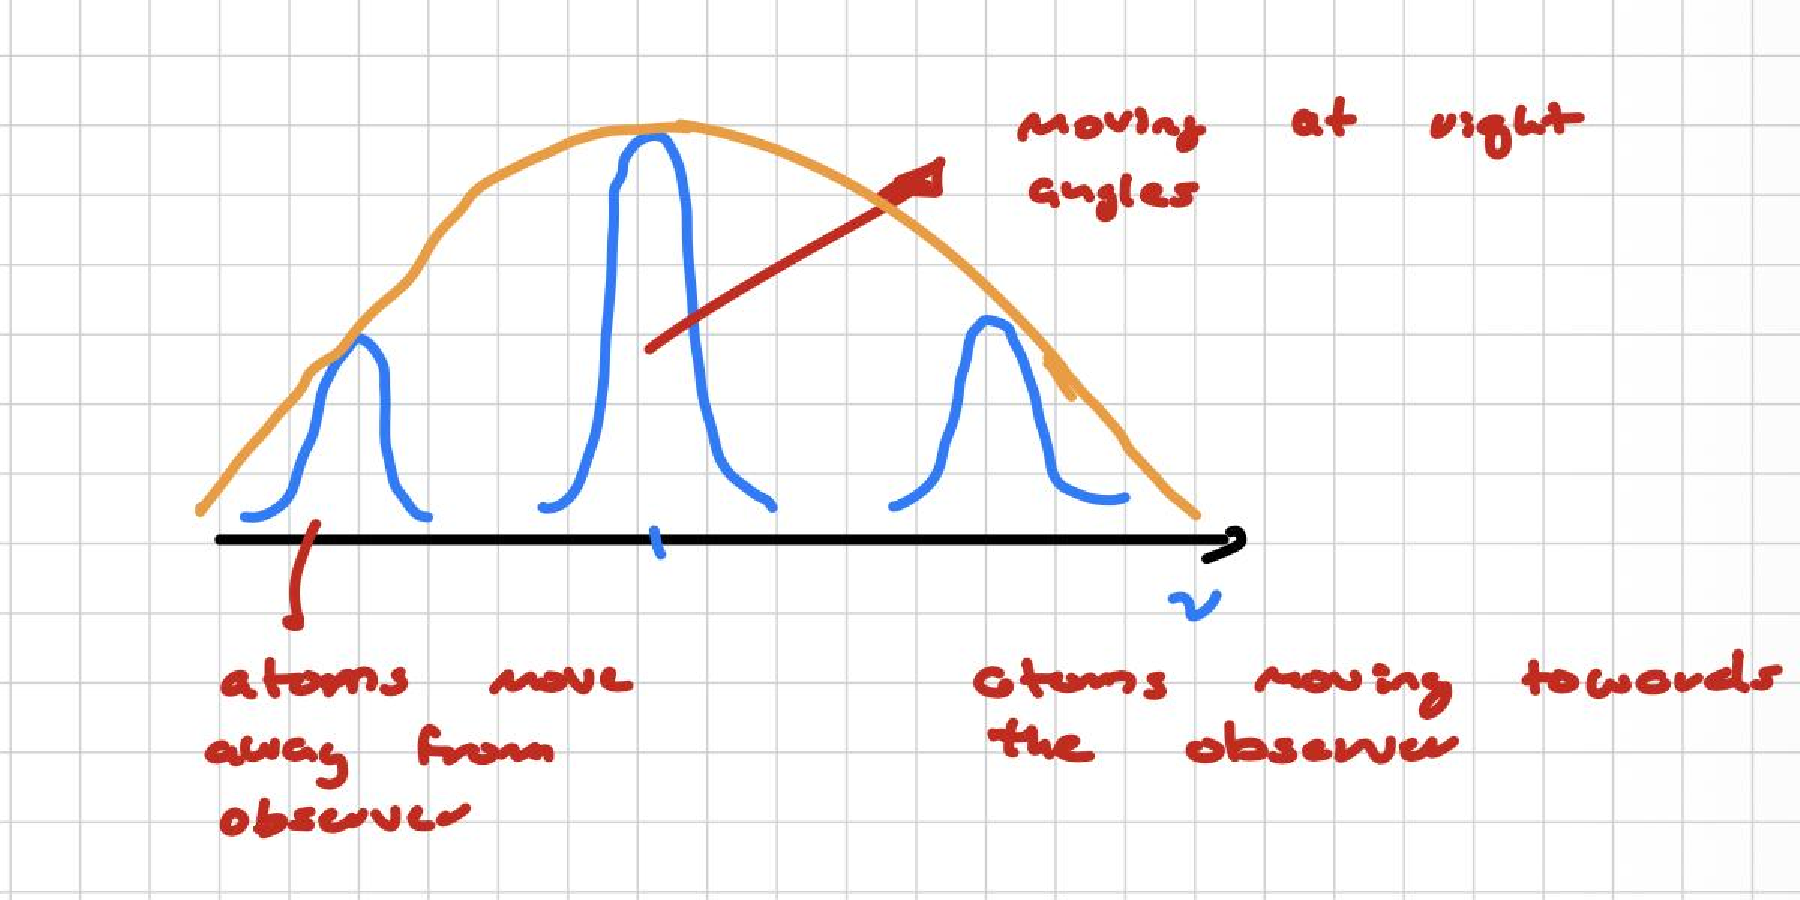
\includegraphics[width=0.8\linewidth]{images_in_pdf/6-/Grafico_24.pdf}
\end{figure}

Each individual atom is assumed to have a naturally broadened emission line, but random thermal motion shifts its central frequency due to the Doppler effect. It is therefore useful to distinguish between two broadening mechanisms:
\begin{itemize}
    \item \textbf{Homogeneous broadening:} \emph{all atoms are affected in the same way}. This is typically due to collision-induced phase interruptions and finite emission lifetime, and leads to a \textbf{Lorentzian line-shape}. It is fundamentally a temporal effect related to the finite coherence time of the emission process.
    \item \textbf{Inhomogeneous broadening:} \emph{different atoms are affected differently}. In this case, each atom emits at a slightly different frequency due to its velocity (Doppler effect), leading to a \textbf{Gaussian line-shape}. This is a statistical effect arising from the distribution of atomic velocities in the ensemble.
\end{itemize}

\subsection{Degree of first-order temporal coherence}

Suppose to come back on \textbf{Mach-Zehnder interferometer}:
\begin{itemize}
    \item We send a complex field $E(t)$ onto a beam splitter (BS), which divides the signal into two paths, $z_1$ and $z_2$ ($z_1 \neq z_2$). Each path contains a mirror and the two beams are then recombined by a second beam splitter, producing two output beams in the directions $E_3(t)$ and $E_4(t)$.
    \item The two beam splitters are identical and have the same \textbf{transmission} coefficient $\tran$ and \textbf{reflection} coefficient $\refl$ ($50{:}50$). These coefficients are also assumed to be independent of the frequency components of the light beam.
\end{itemize}
\begin{figure}[H]
    \centering
    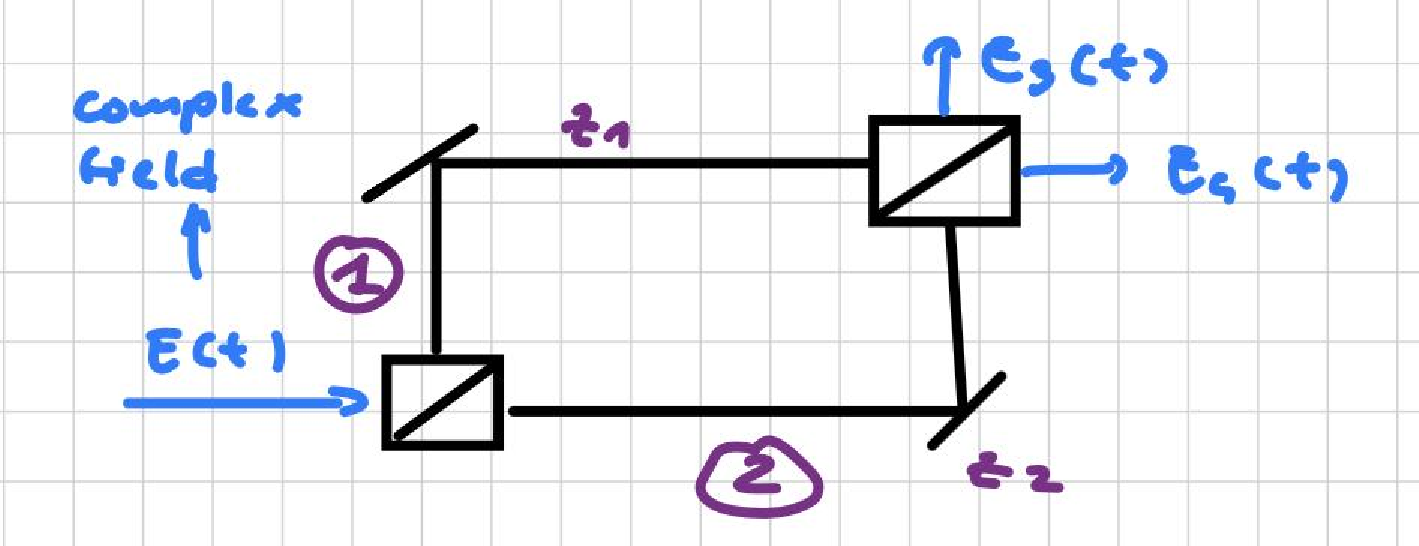
\includegraphics[width=0.8\linewidth]{images_in_pdf/6-/Grafico_25.pdf}
\end{figure}

Along the path $z_1$ we have $\Re[E(t)] = E_1(t)$, while along the path $z_2$ we have $\Re[E(t)] = E_2(t)$. The field reaches the second beam splitter with delays
\begin{equation}\label{eqn:6-delays}
    \Delta t_1 = \frac{z_1}{c}, \qquad \Delta t_2 = \frac{z_2}{c}
\end{equation}

if 
\[
t_1 = t - \frac{z_1}{c}, \qquad t_2 = t - \frac{z_2}{c}.
\]

then,
\begin{equation}\label{eqn:6-field-at-detector}
E_4(t) = \refl\, \tran\, E(t_1) + \tran\, \refl\, E(t_2).
\end{equation}

Averaging over a time window $T \gg \tau_c$, we obtain
\begin{equation}\label{eqn:6-intensity-at-detector}
I_4(t) = \frac{1}{2}\varepsilon_0 c\, \langle|E_4(t)|^2\rangle_T
= \frac{1}{2}\varepsilon_0 c\, |\refl|^2|\tran|^2
\left[
    \langle |E(t_1)|^2\rangle_T + \langle |E(t_2)|^2\rangle_T + 
    2\,\Re \langle E^*(t_1)E(t_2)\rangle_T
\right].
\end{equation}

Notice that the first two terms are the intensities produced by each path separately, in the absence of interference, while the \hl{last term is the interference contribution and is determined by the \textbf{first-order correlation function}}.
\begin{equation}\label{eqn:6-first-order-correlation-function}
\langle E^*(t_1)E(t_2)\rangle_T = \frac{1}{T}\int_T dt_1\,E^*(t_1)E(t_2).
\end{equation}

which is a function only of one variable, since this correlation depends only on the time difference, we define
\[
\tau = t_2 - t_1 = \textbf{fixed quantity},
\]

which means that it depends on the relative delay between the two arms.

If the physical mechanism responsible for the fluctuations does not change in time, then the statistical properties of the light are said to be \textbf{stationary}.
The quantity $\langle E^*(t_1)E(t_2)\rangle_T$ does not depend on the starting time of the averaging interval, provided that $T$ is much larger than the characteristic time of the fluctuations. Since the intensity is obtained by a statistical average over the field values at $t_1$ and $t_2$, the correlation function depends only on $\tau$ and can be written as
\[
\langle E^*(t_1)E(t_2)\rangle_T = \frac{1}{T}\int dt\,E^*(t)E(t+\tau).
\]

We can define the \textbf{degree of first-order temporal coherence} as:
\begin{equation}\label{eqn:6-degree-of-first-order-coherence}
g^{(1)}(\tau) = 
\frac{\langle E^*(t)E(t+\tau)\rangle}{\langle E^*(t)E(t)\rangle} \equiv
\frac{\langle E^*(t)E(t+\tau)\rangle}{\langle |E(t)|^2 \rangle}
\end{equation}

\textbf{which provides a direct measure of how much the electric field remains correlated with itself after a time delay $\tau$.}

Physically, $|g^{(1)}(\tau)|$ quantifies the ability of the field to produce interference: \hl{if $|g^{(1)}(\tau)| \approx 1$, the field is \textbf{highly coherent}} and stable in phase, whereas \hl{if $|g^{(1)}(\tau)| \to 0$}, the field has lost memory of its phase and \hl{\textbf{no interference} can be observed}.

\subsubsection{Correlation in a collision-broadened source}

If we assume a \emph{collision-broadened} light source, the electric field can be written as
\begin{equation}\label{eqn:6-collision-broadened-field}
E(t) = E_0 e^{-i(\omega_0 t + \phi(t))},
\end{equation}

where $E_0$ and $\omega_0$ are constant, while $\phi(t)$ undergoes random changes due to collisions. In this case,
\[
\langle E^*(t)E(t+\tau)\rangle
= E_0^2 e^{-i\omega_0 \tau}
\braket{\left[e^{-i\phi_1(t)} + \cdots + e^{-i\phi_n(t)}\right]
\left[e^{i\phi_1(t+\tau)} + \cdots + e^{i\phi_n(t+\tau)}\right]}.
\]

The \hl{phase angles} associated with different atoms are statistically independent and randomly distributed; therefore, all cross terms \hl{vanish upon averaging}. As a result,
\[
\langle E^*(t)E(t+\tau)\rangle
= E_0^2 e^{-i\omega_0 \tau}\sum_{i=1}^{n} \braket{e^{i[\phi_i(t+\tau)-\phi_i(t)]}}
= n \cdot \langle E_i^*(t)E_i(t+\tau)\rangle.
\]

\calloutinfo{This shows that the total correlation function is entirely determined by the contribution of individual atoms. Physically, this means that coherence is preserved only as long as each atom maintains a well-defined phase during its emission.
After an atom undergoes a collision, its phase is randomized, effectively resetting its contribution to the field. Therefore, the single-atom correlation function is non-zero only if no collision occurs within the time interval $\tau$. In other words, it is \textbf{proportional to the probability that the atom remains in free flight for a time longer than $\tau$.}}

From the kinetic theory of gases, the time between collisions follows an exponential distribution:
\[
\rho(\tau')\,d\tau' = \frac{1}{\tau_0}e^{-\frac{\tau'}{\tau_0}}d\tau',
\]

where $\tau_0$ is the average time between collisions, here $\tau_0=\tau_c$. The probability that no collision occurs in a time interval $\tau$ is then
\[
\int_{\tau}^{\infty} d\tau'\,\rho(\tau') = e^{-\frac{\tau}{\tau_0}}.
\]

As a consequence,
\[
\langle E^*(t)E(t+\tau)\rangle
= E_0^2 e^{-i\omega_0 \tau-\frac{\tau}{\tau_0}},
\]

which shows that the \hl{field loses phase memory exponentially in time}. Finally, the degree of coherence (Eqn.~\ref{eqn:6-degree-of-first-order-coherence}) becomes
\begin{equation}\label{eqn:6-g1-collision-broadened}
g^{(1)}(\tau)
= e^{-i\omega_0 \tau-\frac{|\tau|}{\tau_c}},
\end{equation}

where $\tau_c$ defines the coherence time, i.e. the characteristic time over which the phase of the field remains correlated. This exponential decay directly explains the progressive loss of interference visibility as the time delay between the two paths increases.
\begin{figure}[H]
    \centering
    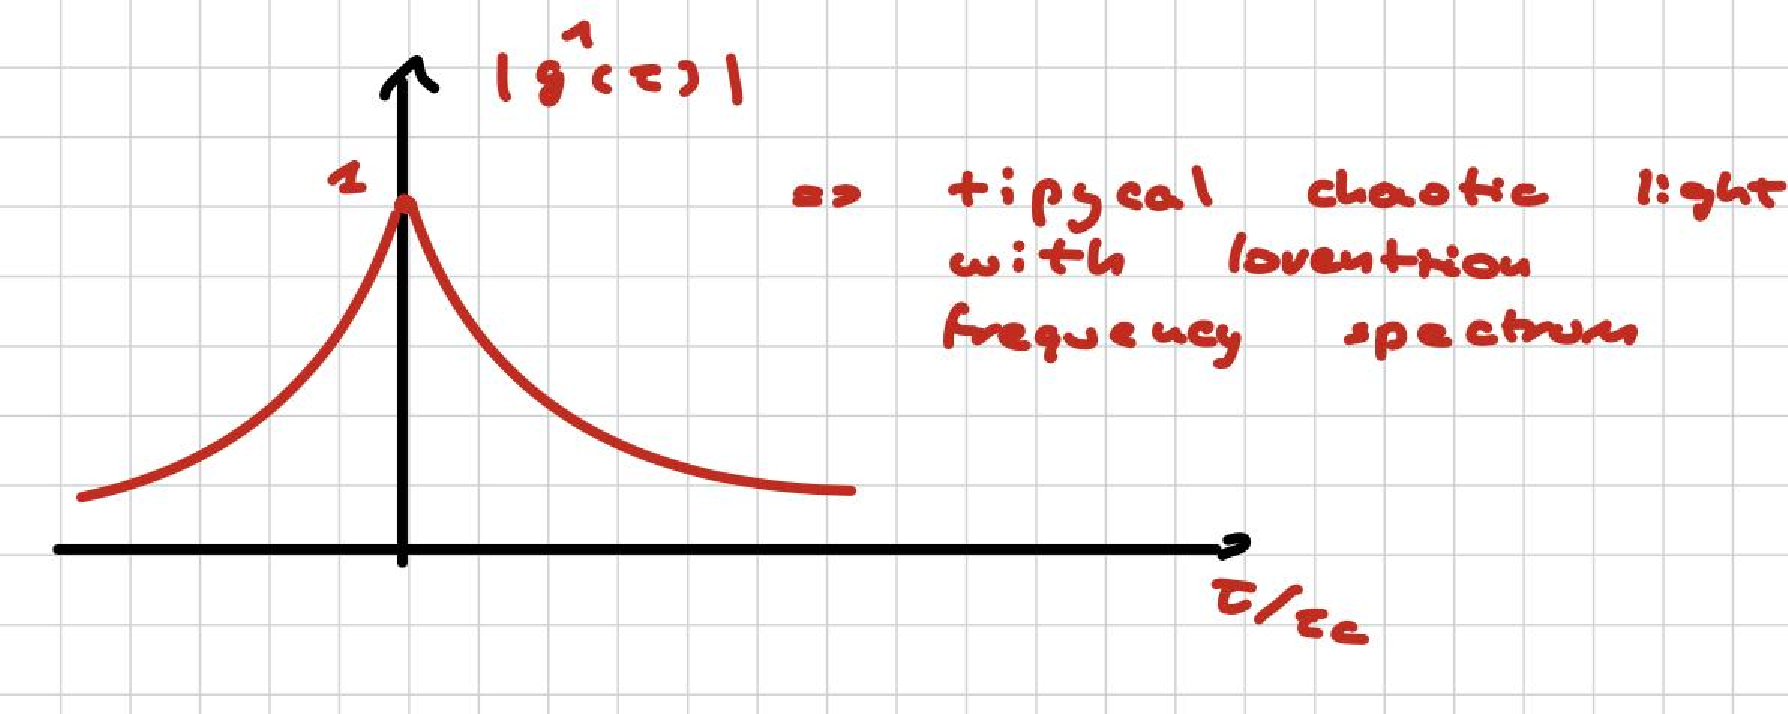
\includegraphics[width=0.8\linewidth]{images_in_pdf/6-/Grafico_26.pdf}
\end{figure}

\subsubsection{Correlation in a Doppler-broadened source}

Similarly, it can be shown that for a \emph{Doppler-broadened} source:
\begin{equation}\label{eqn:6-g1-doppler-broadened}
g^{(1)}(\tau) 
= e^{-i\omega_0\tau-\frac{\pi}{2}\frac{\tau^2}{\tau_c^2}}
\end{equation}
\begin{figure}[H]
    \centering
    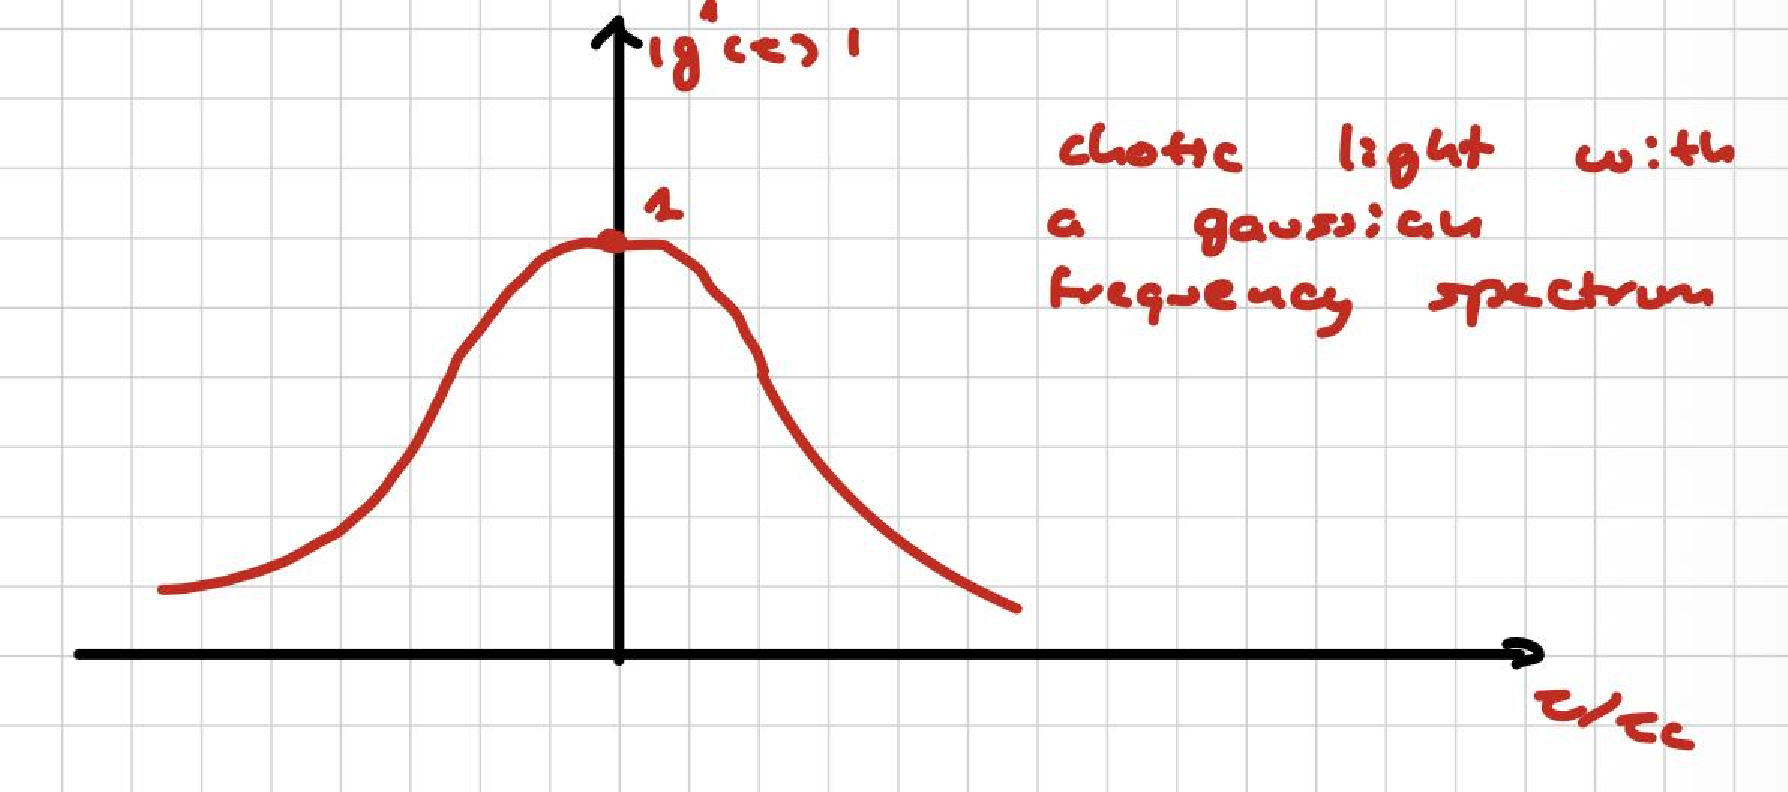
\includegraphics[width=0.8\linewidth]{images_in_pdf/6-/Grafico_27.pdf}
\end{figure}

Observe that:
\begin{itemize}
    \item $g^{(1)}(0)=1$;
    \item light remains first-order coherent for time delays such that $|\tau| \ll \tau_c$.
\end{itemize}

When the delay becomes much larger than the coherence time, the correlation between the fields at $t$ and $t+\tau$ is lost and
\[
\langle E^*(t)E(t+\tau)\rangle \to 0,
\]

so that
\[
g^{(1)}(\tau)\to 0.
\]

\question{What happens if we consider a classical wave with stable amplitude and phase?}{%
\[
E(t)=E_0 e^{-i\omega_0 t+i\phi},
\]

where $\phi$ and $E_0$ are fixed quantities. In this case,
\[
g^{(1)}(\tau)=e^{-i\omega_0\tau}\cdot \langle e^{i[\phi(t+\tau)-\phi(t)]}\rangle.
\]

The first factor is the rapidly oscillating optical phase, with period
\[
T=\frac{2\pi}{\omega_0},
\]

and it gives rise to the interference fringes in the Mach-Zehnder interferometer, while the bracket term contains the coherence information.

For a perfectly coherent light source,
\[
\tau_c\to\infty,
\]

which means that the phase remains correlated for any finite delay. In this ideal case,
\[
|g^{(1)}(\tau)|=1
\]

for all $\tau$.
}

\subsubsection{Correlation in our MZI example}

If we come back on M.Z. interferometer, where we stopped at Equation~\ref{eqn:6-intensity-at-detector}, and average the intensity over a time interval $T$, we obtain:
\[
\begin{split}
    \langle I_4(t)\rangle_T &= 
    \frac{1}{2}\varepsilon_0c\, |\refl|^2|\tran|^2\ 
    \biggl[
        \langle |E(t_1)|^2\rangle_T + \langle |E(t_2)|^2\rangle_T + 
        2\,\Re \langle E^*(t_1)E(t_2)\rangle_T
    \biggr] =\\[0.75ex]
    &= \frac{1}{2}\varepsilon_0c\, |\refl|^2|\tran|^2\ 
    \langle |E(t)|^2\rangle\,
    \left[2+2\,\Re\frac{\langle E^*(t_1)E(t_2)\rangle}{\langle |E(t)|^2\rangle}\right]
\end{split}
\]  

where we have used the fact that the time average of the intensity is the same at $t_1$ and $t_2$ because of stationarity
\begin{equation*}
|E(t_1)| = |E(t_2)| \hspace{0.2cm}\text{through a 50:50 B.S.}
\end{equation*}
finally:
\begin{equation}\label{eqn:6-intensity-at-detector-final}
\langle I_4(t)\rangle_T =
 2\ |\refl|^2|\tran|^2\ \langle I(t)\rangle\,
\left[
    1+\Re\bigl(g^{(1)}(\tau)\bigr)
\right]
\end{equation}

The output intensity is therefore proportional to $\langle I(t)\rangle$ and modulated by the factor $1+\Re(g^{(1)}(\tau))$.

The fringe visibility is given by
\[
V=|g^{(1)}(\tau)|=\frac{I^{\max}-I^{\min}}{I^{\max}+I^{\min}}.
\]

As we've seen in Eqn.~\ref{eqn:6-g1-collision-broadened}, for chaotic light with Lorentzian broadening,
\[
g^{(1)}(\tau)=e^{-i\omega_0\tau-\frac{|\tau|}{\tau_c}},
\]

so that
\[
\langle I_4(t)\rangle=2\, |\refl|^2|\tran|^2\ \langle I(t)\rangle\,
\left[
    1+e^{-\frac{|\tau|}{\tau_c}}\cos(\omega_0\tau)
\right].
\]

This means that when $|\tau|\gg\tau_c$, the fringes disappear.

In conclusion, the first-order temporal coherence and the frequency spectrum are directly related, and they both determine the visibility of interference in optical experiments.

\begin{table}[H]
\label{tab:type-of-light}
\centering
\begin{tabular}{|c|c|c|c|c|}
\hline
Type of light & $\Delta \omega$ & Coherence & $\tau_c$ & $g^{(1)}(\tau_c)$ \\
\hline
Monochromatic & 0 & Perfect & $+\infty$ & 1 \\
\hline
Chaotic & $\Delta \omega$ & Partial & $\sim \frac{1}{\Delta \omega}$ & $0<|g^{(1)}|<1$ \\
\hline
Incoherent & $\infty$ & None & 0 & 0 \\
\hline
\end{tabular}
\end{table}

\section{Photon statistics}\label{sec:photon-statistics}
Intensity fluctuations can be regarded as fluctuations in the number of photons emitted by a source. Because of that, we can use \textbf{photon number distribution function} in order to classify light. In particular we have three type of photon statistics:

\begin{enumerate}
    \item \textbf{Super-Poissonian}: 
    \begin{itemize}
        \item Thermal light, incoherent/ partially coherent light 
        \item $I(t)$ is time dependent
        \item $\Delta n > \sqrt{\overline{n}}$
    \end{itemize}
    \item \textbf{Poissonian}: 
    \begin{itemize}
        \item Perfectly coherent light 
        \item $I(t)$ is constant
        \item $\Delta n = \sqrt{\overline{n}}$
    \end{itemize}
    \item \textbf{Sub-Poissonian}: 
    \begin{itemize}
        \item Not-classical light 
        \item $I(t)$ is constant
        \item $\Delta n <\sqrt{\overline{n}}$
    \end{itemize}
\end{enumerate}

\begin{table}[H]
\label{tab:photon-statistics}
\centering
\begin{tabular}{|c|c|c|c|}
\hline
\textbf{Statistics} & \textbf{Type of light} & \textbf{Intensity $I(t)$} & \textbf{Fluctuations} \\
\hline
Super-Poissonian & Thermal / incoherent (partially coherent) & Time dependent & $\Delta n > \sqrt{\overline{n}}$ \\
\hline
Poissonian & Perfectly coherent & Constant & $\Delta n \approx \sqrt{\overline{n}}$ \\
\hline
Sub-Poissonian & Non-classical light & Constant & $\Delta n < \sqrt{\overline{n}}$ \\
\hline
\end{tabular}

The \hl{first two types of statistics are consistent with classical theory of light}, while the third one leads to quantum description. This happens because light is very sensitive to losses and we need an efficient detective system that it has been observed only recently.

\subsection{Poissonian photon statistics}\label{subsec:poissonian-light}
Suppose we have a \textbf{coherent light} beam:
\[
E(x,t) = E_0 \cdot \cos(kx-\omega_0 t + \phi),
\]

where $E_0$ and $\phi$ are fixed, and $k = \frac{\omega_0}{c}$.\\
The intensity is proportional to $|E(t)|^2$, where $E(t)$ is averaged over an optical cycle. In this case, the intensity is constant in time, which implies that the \textit{average} photon flux is constant.

\question{Is the stream of photons emitted at regular time intervals?}{%
The answer is \textbf{NO}. Even though the intensity is constant, the arrival times of photons exhibit statistical fluctuations on short time scales. A coherent light beam is therefore characterized by \textbf{Poissonian photon statistics}.
}

\textbf{Derivation:}
\begin{proof}
Assume a light beam with constant optical power $P$ and photon flux $\Phi$. Let $\overline{n}$ be the average number of photons within a beam segment of length $L$:
\[
\Phi = \frac{P}{\hbar \omega}, \qquad \overline{n} = \Phi \cdot \frac{L}{c}.
\]

Divide the segment $L$ into $N$ sub-intervals, with $N$ large enough that the probability of finding one photon in a given interval is
\[
p = \frac{\overline{n}}{N},
\]

while the probability of finding more than one photon in the same interval is negligible. The probability of finding $n$ intervals containing one photon and $N-n$ empty intervals is given by the binomial distribution:
\[
\begin{split}
P(n) &= \frac{N!}{n!(N-n)!}\cdot p^n\cdot (1-p)^{N-n} \\
&= \frac{N!}{n!(N-n)!}\cdot \left(\frac{\overline{n}}{N}\right)^n \cdot \left(1-\frac{\overline{n}}{N}\right)^{N-n}.
\end{split}
\]

In the limit $N \to \infty$, this expression converges to the \textbf{Poisson distribution}:
\begin{equation}\label{eqn:7-poisson-distribution}
P(n) = \frac{1}{n!}\cdot (\overline{n})^n\cdot e^{-\overline{n}}, \qquad n=0,1,2,\dots
\end{equation}

\end{proof}

Notice that:
\begin{itemize}
    \item The distribution peaks around $\overline{n}$;
    \item The variance is
    \[
    (\Delta n)^2 \coloneqq \sigma^2 = \sum_{n=0}^{\infty} (n-\overline{n})^2 P(n) = \overline{n};
    \]
    \item Standard deviation is
    \[
    \Delta n \coloneqq \sigma = \sqrt{\overline{n}},
    \]
    which shows that fluctuations increase with the mean photon number, while the relative fluctuations decrease as $1/\sqrt{\overline{n}}$.
\end{itemize}
\subsection{Super Poissonian light}\label{subsec:7-super-poissonian-light}

\subsubsection{Black body behavior}\label{subsubsec:7-black-body-behavior}

A \textbf{black body} can be modeled as an \textbf{enclosed cavity at temperature $T$} filled with electromagnetic radiation. In this case, the field consists of a continuous spectrum of oscillating modes with \textbf{energy density} $\rho(\omega,T)$, where $\omega$ is the angular frequency of a given mode. Each mode behaves as a quantized harmonic oscillator with energy:
\begin{equation}\label{eqn:7-energy-of-a-mode}
E_n=\hbar\omega\left(n+\frac{1}{2}\right).
\end{equation}

This leads to the Planck distribution:
\[
\rho(\omega,T)\ \d\omega = \frac{\hbar \omega^3}{\pi^2 c^3}\  
\frac{1}{e^{\beta \hbar \omega}-1}\ \d\omega.
\]

According to Boltzmann statistics, the probability that there are $n$ photons in a single mode of angular frequency $\omega$ is

\begin{equation}
P_{\omega}(n) = 
\frac{e^{-\beta E_n}}{\sum_{n=0}^{\infty} e^{-\beta E_n}}= 
\frac{e^{-\beta \cdot \hbar \omega \cdot n}}
{\sum_{n=0}^{\infty} e^{-\beta \cdot \hbar \omega \cdot n}}
\end{equation}

which is something in the form of $\frac{x^n}{\sum x^n}$, where:
\begin{equation}
\sum x^n = \frac{1}{1-x}, \qquad x=e^{-\beta\hbar\omega}
\end{equation}

so that:
\begin{equation}
P_{\omega}(n) = 
e^{-\beta\cdot \hbar \omega \cdot n}\  
\left(1-e^{-\beta\cdot \hbar \omega}\right),
\end{equation}

\begin{figure}[H]
    \centering
    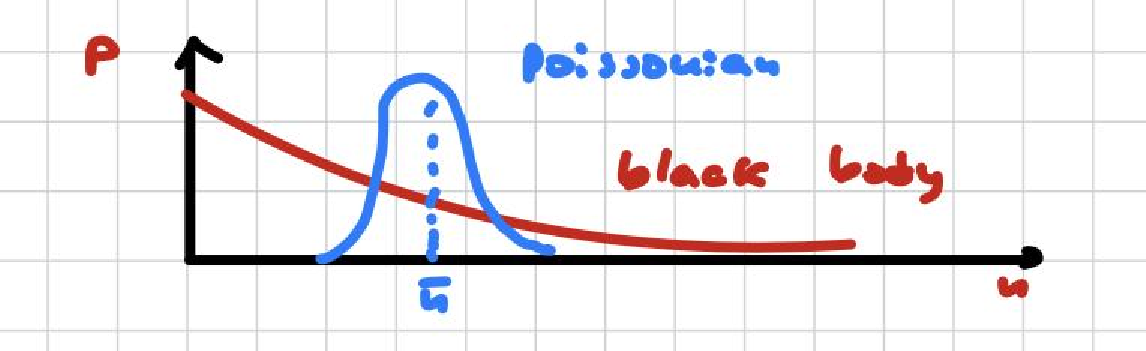
\includegraphics[width=0.8\linewidth]{images_in_pdf/7-/Grafico_28.pdf}
\end{figure}

Observe that the maximum of the distribution is at $n=0$ and that the probability decreases exponentially with $n$. From this expression one obtains the mean photon number and the \textbf{Bose-Einstein distribution}:
\[
P_{\omega}(n)= \frac{1}{\overline{n}+1}\cdot \left(\frac{\overline{n}}{\overline{n}+1}\right)^n,
\qquad
\overline{n}=\frac{1}{e^{\beta\hbar\omega}-1}.
\]

The variance is
\[
\sigma^2 = (\Delta n)^2 = \overline{n}+\overline{n}^2,
\]

hence:
\begin{equation}\label{eqn:7-super-poissonian-variance}
(\Delta n)^2_{\text{Bose}} > (\Delta n)^2_{\text{Poissonian}}.
\end{equation}

The fluctuations are therefore larger than in the Poissonian case, which means that the photon-number distribution of thermal light is broader than that of coherent light. Thermal light is thus \textbf{super-Poissonian}.

\calloutwarn{%
\textbf{Be aware!} The Bose-Einstein distribution applies to a single mode, whereas a black body contains a continuum of modes. If many independent modes are collected in the same detection time, the bunching contribution is reduced. In a multimode measurement one often writes
\[
(\Delta n)^2 = \overline{n}+\frac{\overline{n}^2}{M},
\]
where $M$ is the number of independent modes contributing to the detected signal; in the limit $M\to\infty$, the excess fluctuation term is suppressed and the statistics can approach Poissonian behavior. In a real experiment, observing a strictly single-mode thermal field is difficult, because mode averaging and interference effects tend to wash out part of the bunching signal.
}

\subsubsection{Discharge lamp behavior}\label{subsubsec:7-discharge-lamp-behavior}

Suppose we have a discharge lamp with a single spectral line. Such a source is a chaotic light source, meaning that it exhibits classical intensity fluctuations on a timescale set by the coherence time $\tau_c$. The fluctuations in the photon number, when the flux is measured over a detection time $T$, are given by
\begin{equation}\label{eqn:7-fluctuations-discharge-lamp}
(\Delta n)^2 = \langle W(T)\rangle + \langle \delta W(T)^2\rangle.
\end{equation}

\hl{The first term comes from \textbf{Poissonian shot noise}, which reflects the particle nature of light, while the second term represents classical power fluctuations}.

Here:
\begin{itemize}
    \item $W(T)$ is the count rate within a detection time $T$:
    \[
    W(T) = \int_t^{t+T} \eta \, \Phi(t')\,dt',
    \]
    \item $\eta$ is the detection efficiency,
    \item $\Phi = \frac{P}{\hbar\omega}$ is the instantaneous photon flux,
    \item $\delta W(T) = W(T)-\langle W(T)\rangle$ denotes the classical fluctuation of the detected signal.
\end{itemize}

Notice that if $\Phi$ is constant, then
\[
\langle \delta W(T)^2\rangle = 0
\]

and one recovers the Poissonian result
\[
(\Delta n)^2 = \overline{n}.
\]

In our case, however, $\Phi \neq \text{constant}$ and \textbf{two different regimes} can be identified:

\begin{enumerate}
    \item \emph{The intensity fluctuations are relevant when}
    \begin{equation}\label{eqn:7-fluctuations-relevant}
    T \leq \tau_c \implies \langle \delta W(T)^2\rangle \neq 0.
    \end{equation}

    In this regime, the \hl{detection time is short enough that the detector can resolve the temporal fluctuations of the light field}. Since the phase and intensity remain correlated over a time of order $\tau_c$, the measured signal reflects not only the Poissonian shot noise (due to the particle nature of light), but also the classical intensity fluctuations of the source. Physically, this corresponds to the fact that thermal light exhibits photon bunching, so photons tend to arrive in correlated groups rather than independently.
    \item \emph{The Poissonian behavior is approached when}
    \begin{equation}\label{eqn:7-poissonian-limit}
    T > \tau_c \implies \Phi \approx \text{constant}.
    \end{equation}

    In this case, the detector integrates the signal over many independent coherence intervals. As a result, the rapid phase and intensity fluctuations average out, and the contribution of classical power fluctuations is strongly reduced:
    \[
    \langle \delta W(T)^2\rangle \to 0.
    \]
    The measured statistics therefore approaches the Poissonian limit, where fluctuations are dominated by shot noise. Physically, \hl{this does not mean that the light itself becomes Poissonian, but rather that the measurement process averages over the fluctuations, making the detected signal appear more regular}.
\end{enumerate}
\subsection{Sub-Poissonian light}
By definition $\Delta n < \sqrt{\overline{n}}$, it has not a classical equivalent and it is a clear signature of quantum nature of light.

Suppose to have a light beam where every time interval between the photons is the same $\Delta x = c \Delta t$. In a time $T$ the photocount will be:
\begin{equation}\label{eqn:7-sub-poissonian-photocounts}
N = \mathrm{int} 
\biggr(
    \eta \cdot \frac{T}{\Delta t}
\biggr)
\end{equation}
\begin{figure}[H]
    \centering
    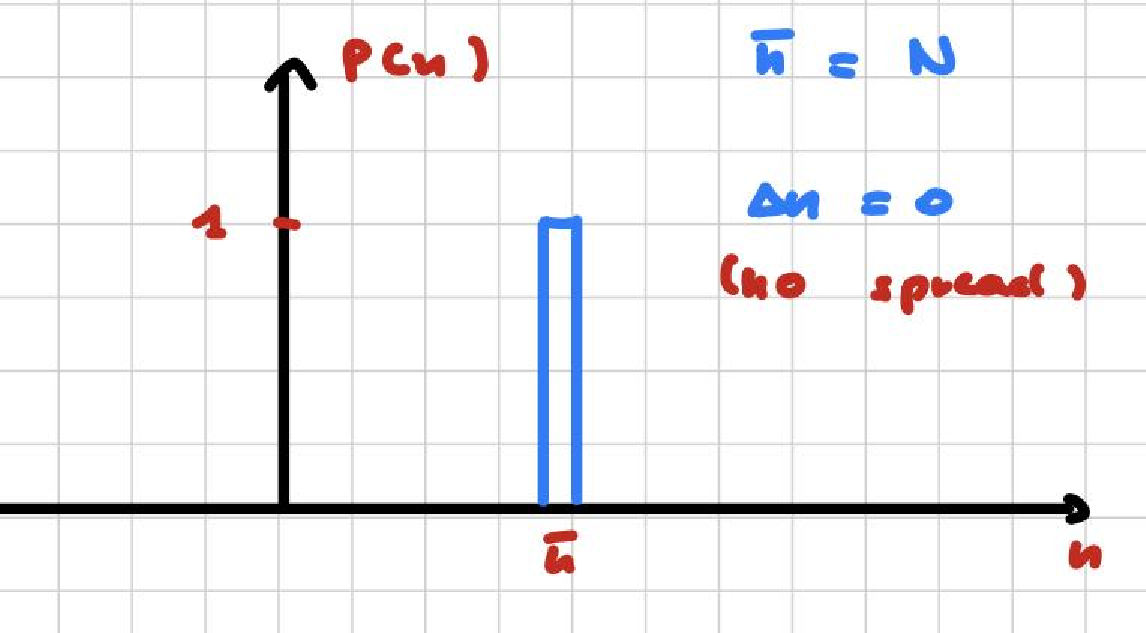
\includegraphics[width=0.8\linewidth]{images_in_pdf/7-/Grafico_29.pdf}
\end{figure}

This kind of photon stream is called \textbf{Photon Number states}. Observe that the time intervals $\Delta t$ are not exactly the same, but more \say{regular} than the random intervals pertaining to beams having poissonian statistics.

\calloutwarn{%
Sub-poissonian instead is very fragile and for this reason we need to avoid optical losses and have high-efficiency detectors.

The main factors that degrade photon statistics are:
\begin{itemize}
    \item Inefficient collection of light emitted by source;
    \item Absorption/scattering/reflection from optical components;
    \item Imperfect quantum detection.
\end{itemize}
}

\hl{This leads us to study photodetection}.

\subsubsection{Photodetection}\label{subsubsec:7-photodetection}

\question{How are the electric field and light intensity converted into an experimental signal?}{%
Photodetectors operate by absorbing a portion of the incoming light beam and converting its energy into a measurable electrical signal.}

For example, consider a red laser with wavelength $\lambda = \qty{633}{\nano\meter}$ and a very low power $P \approx \qty{1}{\nano\watt}$; the \textbf{photon flux} impinging on the detector is still huge:
\begin{equation}\label{eqn:7-photon-flux-example}
\Phi = \frac{IA}{\hbar \omega} = \frac{P}{\hbar \omega} \approx 3\cdot 10^9 \ \text{photons/s}.
\end{equation}

This high photon flux motivates the use of devices capable of counting individual photons within a given time interval $\Delta t$: \textbf{photon counters}.

We can define:

\begin{itemize}
\item  the \textbf{quantum efficiency} of the detector, or probability that an incident photon produces a photocount:
\begin{equation}\label{eqn:7-quantum-efficiency}
\eta = \frac{\text{Number of photocounts}}{\text{Number of incident photons}};
\end{equation}

\item  the \textbf{average number of counts} recorded during a time interval $T$: 
\begin{equation}\label{eqn:7-average-counts}
M(T) = \eta \cdot \Phi \cdot T = \eta \cdot \frac{P}{\hbar \omega} \cdot T;
\end{equation}

\item the corresponding \textbf{average count rate}:
\begin{equation}\label{eqn:7-average-count-rate}
R = \frac{M(T)}{T} = \eta \cdot \frac{P}{\hbar \omega} \quad [\text{counts/s}].
\end{equation}

\end{itemize}

\calloutwarn{If the detector has a \textbf{dead time}, which is a recovery period after each detection event, this limits the maximum count rate. For instance, a dead time of \qty{1}{\nano\second} determines a \emph{maximum rate} of $R \approx 10^9$ counts/s.}

It is also important to observe that $R$ and $\Phi$ are \textbf{average quantities}, while the actual photon flux exhibits statistical fluctuations due to the discrete nature of light. \hl{These fluctuations of the measured count rate $R$ can be used to study the photon statistics of the light beam.}

However, in addition to the intrinsic photon statistics of the light, \textbf{the detector itself introduces fluctuations because the detection process is probabilistic:}
\begin{itemize}
    \item Each photon is registered with probability $\eta$, so the photocounts follow a \textbf{Bernoulli process} for each incident photon.
    \item Additional sources of fluctuation include dark counts, electronic noise, dead time effects, and imperfect detection efficiency.
\end{itemize}
As a result, the observed photocounts reflect both the \hl{statistical properties of the light beam} and the \hl{stochastic nature of the detection process}. Therefore, when analyzing photon statistics, it is essential to distinguish between fluctuations due to the light source itself and those introduced by the detector.
\subsubsection{Semiclassical theory}
In order to study photo-counting detectors, we start with the photomultiplier.
\begin{figure}[H]
    \centering
    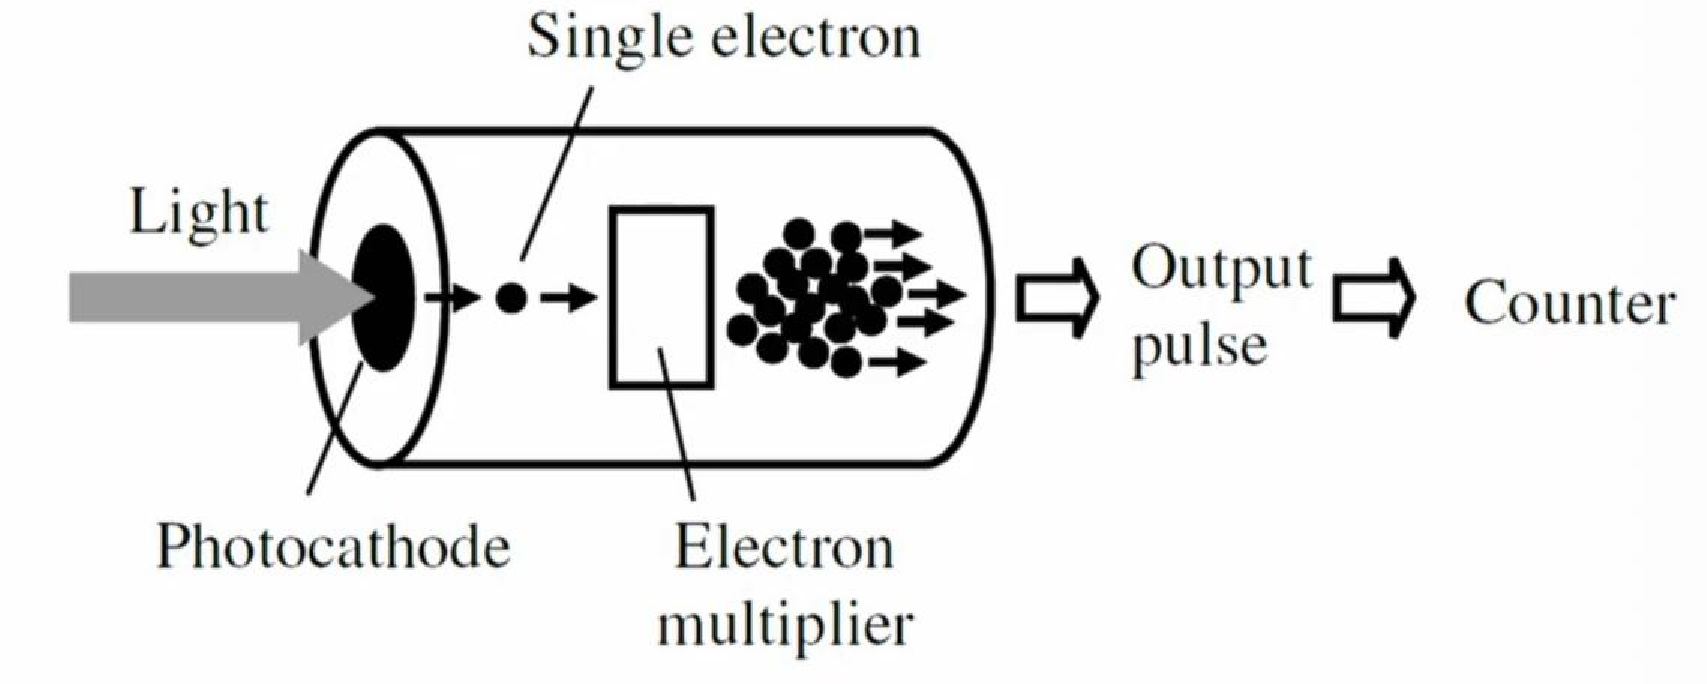
\includegraphics[width=0.8\linewidth]{images_in_pdf/7-/Grafico_30.pdf}
\end{figure}

Suppose that a light beam impinges on a photocathode, so that a single electron is emitted by the \textbf{photoelectric effect} and then amplified by an electron multiplier. This process gives rise to an output pulse and, consequently, to a count.

\hl{In the semiclassical framework, atoms and the detector are treated quantum mechanically, while the electromagnetic field is treated classically}. The number of photocounts produced in an integration time $T$ is therefore a measure of the optical intensity. We consider a large number of successive measurements, each performed over the same integration time, in order to build the probability distribution $P_n(T)$ for observing $n$ photocounts during the interval $T$.

The probability that the light causes the emission of one electron, observed as a photocount event between $t$ and $t+dt$, is
\[
p(t)\,dt = \eta\,I(t)\,dt,
\]
where $\eta$ is the detector efficiency and $I(t)$ is the appropriately normalized light intensity. We assume $dt$ to be sufficiently small so that the probability of detecting two electrons in the same interval is negligible.

If we define $P_n(t,\tau)$ as the probability that $n$ photocounts occur in the time interval from $t$ to $t+\tau$, then, after a further short interval $d\tau$, the same $n$ photocounts can be obtained in two ways:

\begin{equation}\label{eqn:7-photon-statistics-derivation}
\begin{split}
    a&.
    \begin{cases}
    a_1.\ n \text{ events} \hspace{0.55cm} &t \to t+\tau\\
    a_2.\ 0 \text{ events}              &t+\tau \to t+\tau+d\tau
    \end{cases}
    \\[1ex]
    b&.
    \begin{cases}
        b_1.\ n-1 \text{ events} &t \to t+\tau\\
        b_2.\ 1 \text{ event}    &t+\tau \to t+\tau+d\tau
    \end{cases}
\end{split}
\end{equation}

hence:
\begin{equation}\label{eqn:7-photon-statistics-probabilities}
\begin{alignedat}{3}
    a&.
    \begin{cases}
        P(a_1) = P_n(t,\tau)\\
        P(a_2) = 1 - p(t+\tau)\,\d\tau
    \end{cases}
    &&\implies\ 
    P(a) = P_n(t,\tau) \left[1 - p(t+\tau)\,\d\tau\right]
    \\[1ex]
    b&.
    \begin{cases}
        P(b_1) = P_{n-1}(t,\tau)\\
        P(b_2) = p(t+\tau)\,\d\tau
    \end{cases}
    &&\implies\ 
    P(b) = P_{n-1}(t,\tau)\,p(t+\tau)\,\d\tau
\end{alignedat}
\end{equation}

The total probability is then
\begin{equation}\label{eqn:7-photon-statistics-total-probability}
\begin{split}
    P_n(t,\tau+d\tau) &= P_n(t,\tau)\,[1-p(t+\tau)\,d\tau] + P_{n-1}(t,\tau)\,p(t+\tau)\,d\tau\\
    &= P_n(t,\tau) - \eta I(t+\tau)P_n(t,\tau)\,d\tau + \eta I(t+\tau)P_{n-1}(t,\tau)\,d\tau,
\end{split}
\end{equation}

which gives
\[
\frac{dP_n(t,\tau)}{d\tau}=\eta\,I(t+\tau)\,[P_{n-1}(t,\tau)-P_n(t,\tau)].
\]

For $n=0$, the term $P_{-1}$ vanishes, so
\[
\frac{dP_0(t,\tau)}{d\tau}=-\eta\,I(t+\tau)\,P_0(t,\tau).
\]

Since there are no photocounts in a zero-time interval, the boundary conditions are
\[
P_0(t,0)=1, \qquad P_n(t,0)=0 \quad \forall\, n\ge 1.
\]

Using these boundary conditions and solving recursively, we obtain the \textbf{Mandel formula}
\[
P_n(t,T)=\frac{1}{n!}\left[\eta \int_t^{t+T} I(t')\,dt'\right]^n
\exp\!\left[-\eta \int_t^{t+T} I(t')\,dt'\right].
\]

If we define the average intensity over the integration time as
\[
I(t,T)=\frac{1}{T}\int_t^{t+T} I(t')\,dt',
\]

then the formula can be written as
\[
P_n(t,T)=\frac{1}{n!}\,[\eta\,I(t,T)\,T]^n\,e^{-\eta\,I(t,T)\,T},
\qquad
P_0(t,T)=e^{-\eta\,I(t,T)\,T}.
\]

It can also be shown that
\[
\overline{n}=\sum_n n\,P_n(t,T)=\eta\,\langle I(t,T)\rangle\,T.
\]

From here, we have two scenarios:

\textbf{1} Classical stable wave:
\[
\langle I(t,T)\rangle=\text{constant} \implies \eta\,\langle I\rangle = C.
\]

We can calculate $P_n$ in the limit $d\tau \to 0$:
\[
\frac{dP_n}{d\tau}=C\,[P_{n-1}-P_n] \implies \frac{dP_n}{d\tau}+C\,P_n=C\,P_{n-1}.
\]

If $n=0$, then $P_{n-1}=0$, and therefore
\[
\begin{cases}
\frac{dP_0}{d\tau}=-C\,P_0\\
P_0(0)=1
\end{cases}
\implies P_0(T)=e^{-CT}.
\]

For $n\ge 1$, using the integrating factor $e^{CT}$, we obtain
\[
\frac{d}{d\tau}\!\left[P_n(\tau)e^{C\tau}\right]=C\,P_{n-1}(\tau)e^{C\tau},
\]

so that
\[
P_n(T)=e^{-CT}\int_0^T d\tau\, C\,e^{C\tau}\,P_{n-1}(\tau).
\]

We can solve this recursively:
\[\begin{split}
    P_1(T) &= e^{-CT}\int_0^T d\tau\, C\,e^{C\tau}\,P_0(\tau)
    = e^{-CT}\int_0^T d\tau\, C
    = e^{-CT}\,CT,\\
    P_2(T) &= e^{-CT}\int_0^T d\tau\, C\,e^{C\tau}\,P_1(\tau)
    = e^{-CT}\,\frac{(CT)^2}{2},\\
    P_n(T) &= e^{-CT}\,\frac{(CT)^n}{n!}.
\end{split}\]

Since
\[
\overline{n}=\eta\,\langle I\rangle\,T=CT,
\]

we finally obtain
\[
P_n(T)=\frac{\overline{n}^{\,n}}{n!}\,e^{-\overline{n}}.
\]

\calloutinfo{Thus, we recover the Poisson distribution, which means that the photocount statistics are the same as those of particle emission in radioactive decay.

A measurement of the continuous time-dependent intensity of a classical wave by means of a photomultiplier produces discrete photocounts with a well-defined distribution.}

Observe that we obtain Poissonian statistics without invoking photons explicitly, we only assume that
\begin{itemize}
    \item emission of photoelectrons is probabilistic;
    \item light energy is absorbed in discrete detection events.
\end{itemize}
However, \textbf{the photocount statistics do not, by themselves, reveal the full quantum nature of light. A classical field with constant intensity leads to Poissonian counting, while sub-Poissonian statistics require a more general quantum theory of the electromagnetic field.}
\subsubsection{Quantum theory of photodetection}
Assume that we have:
\begin{itemize}
    \item The variance of the photocount number is
    \[
    (\Delta N)^2 = \eta^2 (\Delta n)^2 + \eta(1-\eta)\,\overline{n},
    \]
    The first term in the variance,
\[
\eta^2 (\Delta n)^2,
\]
represents the fluctuations already present in the incoming light, reduced by the finite efficiency of the detector. The second term,
\[
\eta(1-\eta)\,\overline{n},
\]
is the additional noise introduced by the detection process itself, due to the random loss of photons. \\
    \item The quantum efficiency is
    \[
    \eta = \frac{\overline{N}}{\overline{n}},
    \]
    where $\overline{N}$ is the average photocount number and $\overline{n}$ is the mean photon number impinging on the detector.
\end{itemize}
We can have:
\begin{enumerate}
    \item If $\eta = 1$, then $\Delta N = \Delta n$, so the photon counts faithfully reproduce the fluctuations of the incident photon stream.\\
    \item If $(\Delta n)^2 = \overline{n}$, i.e. the incident light has Poissonian statistics, then
    \[
    (\Delta N)^2 = \eta \overline{n} = \overline{N} \qquad \forall\, \eta,
    \]
    which means that the photocount fluctuations remain Poissonian.
\end{enumerate}
\textbf{A detector with efficiency $\eta$ can be modeled as a perfect detector preceded by a beam splitter of transmittance $\eta$}, which randomly selects which photons are actually detected, independently of the original state of light. In this sense, the detection process is equivalent to a binomial thinning of the incident photon number distribution. \\\\
\textbf{If $\eta \ll 1$, the detected photocount stream becomes strongly randomized and tends toward Poissonian statistics}, even if the original light state had reduced fluctuations. For this reason, \textbf{low quantum efficiency tends to mask sub-Poissonian behavior} and makes it difficult to observe nonclassical light experimentally. \\
In practice, it is difficult to realize detectors with very high quantum efficiency ($\eta > 50\%$), and this is one of the reasons why observing sub-Poissonian statistics is experimentally challenging.
\subsubsection{Quantum noises}
Let us start with \textbf{photodiodes}. Consider a $p$-$n$ junction under reverse bias. When external light impinges on the junction, it generates electron-hole pairs, which are then separated by the electric field and collected at the contacts. This process gives rise to a \textbf{photocurrent} $i$: 
\begin{figure}[H]
    \centering
    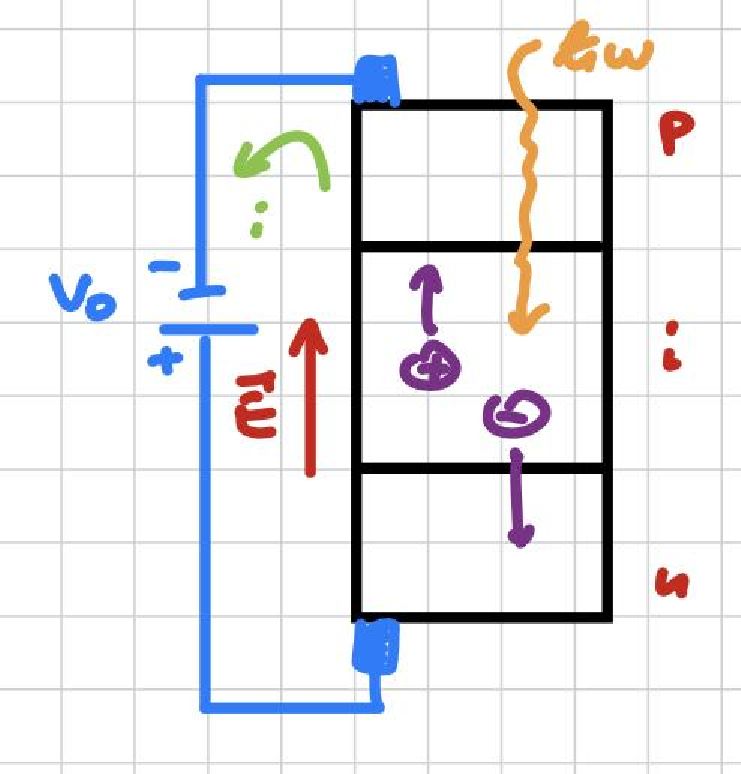
\includegraphics[width=0.5\linewidth]{images_in_pdf/7-/Grafico_31.pdf}
\end{figure}

The \textbf{photodiode responsivity} can be defined as
\[
i = \eta\,|e|\,\Phi = \eta\,|e|\,\frac{P}{\hbar\omega}
\qquad \Rightarrow \qquad
\frac{i}{P} = \eta\,\frac{|e|}{\hbar\omega}
\hspace{0.5cm}\left[\frac{A}{W}\right],
\]
where $\Phi$ is the photon flux, $P$ is the optical power, and $\eta$ is the quantum efficiency. More precisely, the responsivity depends on wavelength through $\hbar\omega = hc/\lambda$, so that
\[
\frac{i}{P}=\eta\,\frac{|e|\lambda}{hc}.
\]
We now connect the photodiode to a load resistor and measure the output voltage $V(t)$ using an amplifier and filtering the signal. The photocurrent produces
\[
V(t)=i(t)\,R_L.
\]
\begin{figure}[H]
    \centering
    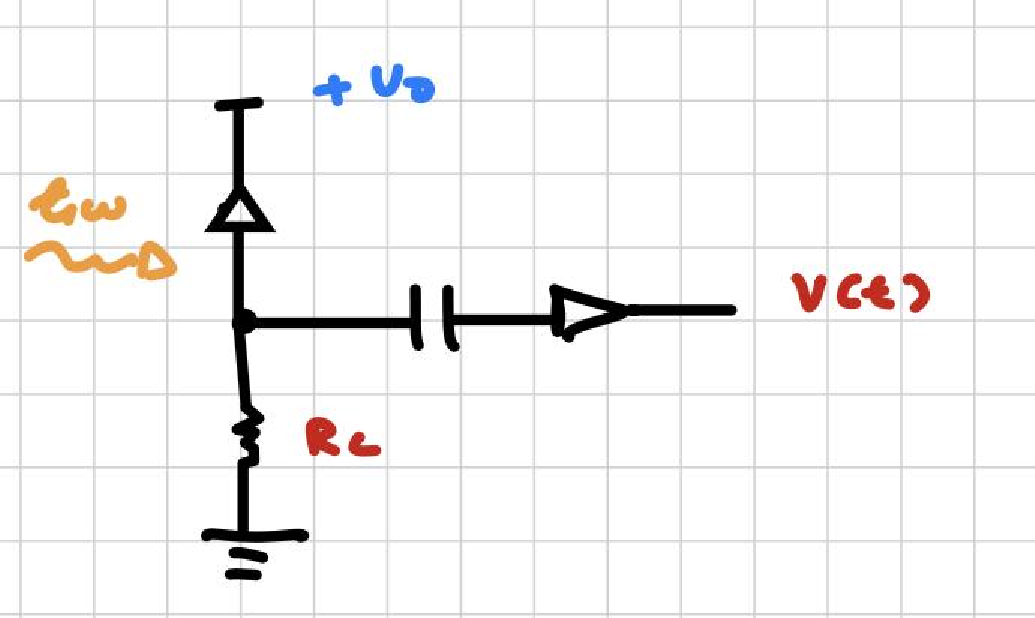
\includegraphics[width=0.8\linewidth]{images_in_pdf/7-/Grafico_32.pdf}
\end{figure}

The measured current can be decomposed into a mean value and a fluctuation:
\[
i(t)=\langle i(t)\rangle+\Delta i(t).
\]
\begin{figure}[H]
    \centering
    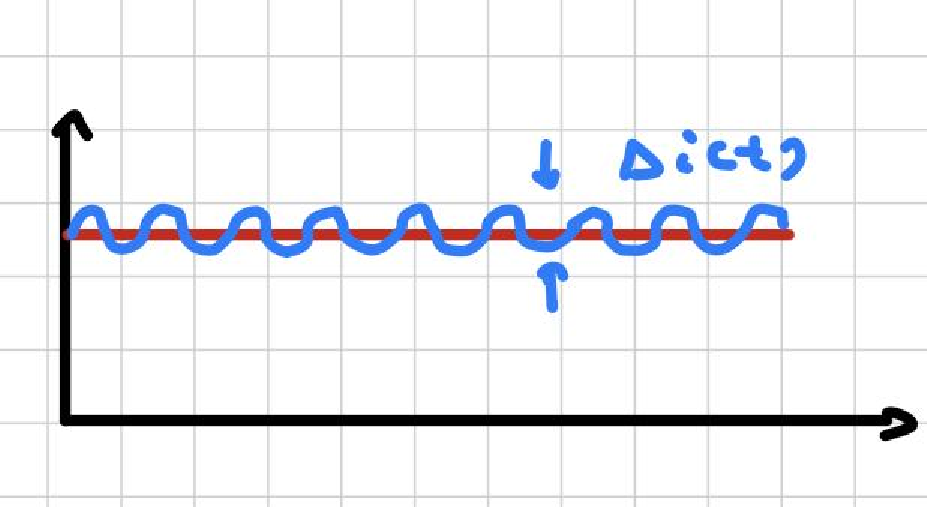
\includegraphics[width=0.8\linewidth]{images_in_pdf/7-/Grafico_33.pdf}
\end{figure}

If the number of detected photons fluctuates, then the photocurrent fluctuates as well, with a detection fidelity set by $\eta$. These fluctuations are precisely the noise:
\[
\langle \Delta i(t)\rangle = 0
\qquad \text{but} \qquad
\langle \Delta i^2(t)\rangle \neq 0.
\]
This is reflected in the electrical power dissipated on the load. In a time-domain description one may write
\[
P_{\text{noise}}(t)=\Delta i^2(t)\,R_L,
\]
while in a frequency-domain treatment it is more precise to consider the noise spectral density of the current or voltage. The decibel scale is
\[
P[\text{dBm}] = 10\log_{10}\!\left(\frac{\text{power}}{1\,\text{mW}}\right).
\]
If we analyze the noise in the frequency domain by Fourier transforming the signal, we can distinguish two different regions:
\begin{figure}[H]
    \centering
    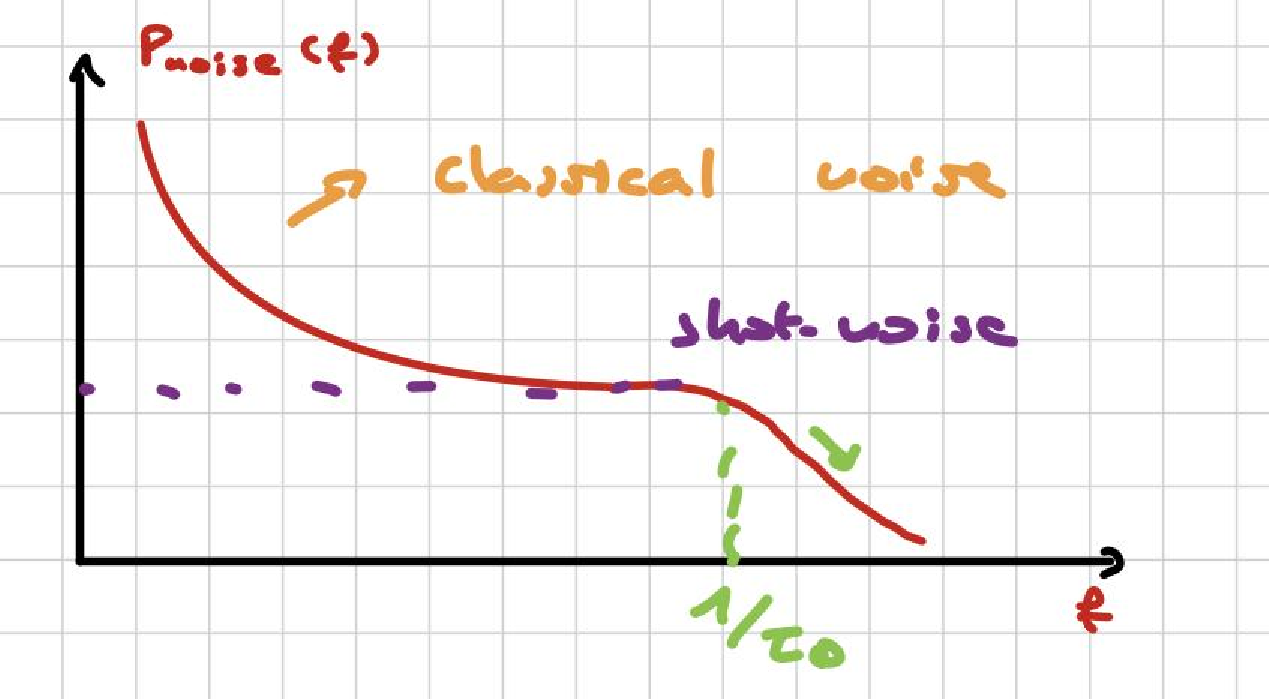
\includegraphics[width=0.8\linewidth]{images_in_pdf/7-/Grafico_34.pdf}
\end{figure}
\newpage
\begin{itemize}
    \item \textbf{Low-frequency limit:} this region is dominated by technical noise, such as fluctuations in the electrical drive current, laser intensity noise, and mechanical vibrations of the optical cavity. In this regime we have \textbf{classical noise}.\\
    \item \textbf{High-frequency limit:} here the technical noise is suppressed and only the fundamental noise associated with photon statistics remains. In this regime we have \textbf{shot noise} or \textbf{quantum noise}.\\
    \item \textbf{High-frequency cut-off:} the noise spectrum eventually decreases to zero because of the finite \textbf{detection response time} $\tau_D$, which limits the bandwidth of the detector.
\end{itemize}
If we consider an ideal coherent light source, we know that the photon statistics are Poissonian. This is reflected in the number of photogenerated charges, for which
\[
(\Delta N)^2 = \langle N\rangle.
\]
Since the photocurrent is proportional to the number of detected charges, the current fluctuations satisfy
\[
(\Delta i)^2 \propto \langle i(t)\rangle,
\]
and therefore
\[
P_{\text{noise}} = (\Delta i)^2\,R_L \propto \langle i(t)\rangle \propto P_{\text{optical}}.
\]
This means that there is a linear relation between noise power and optical power. For a coherent source, this is the hallmark of shot noise:
\begin{figure}[H]
    \centering
    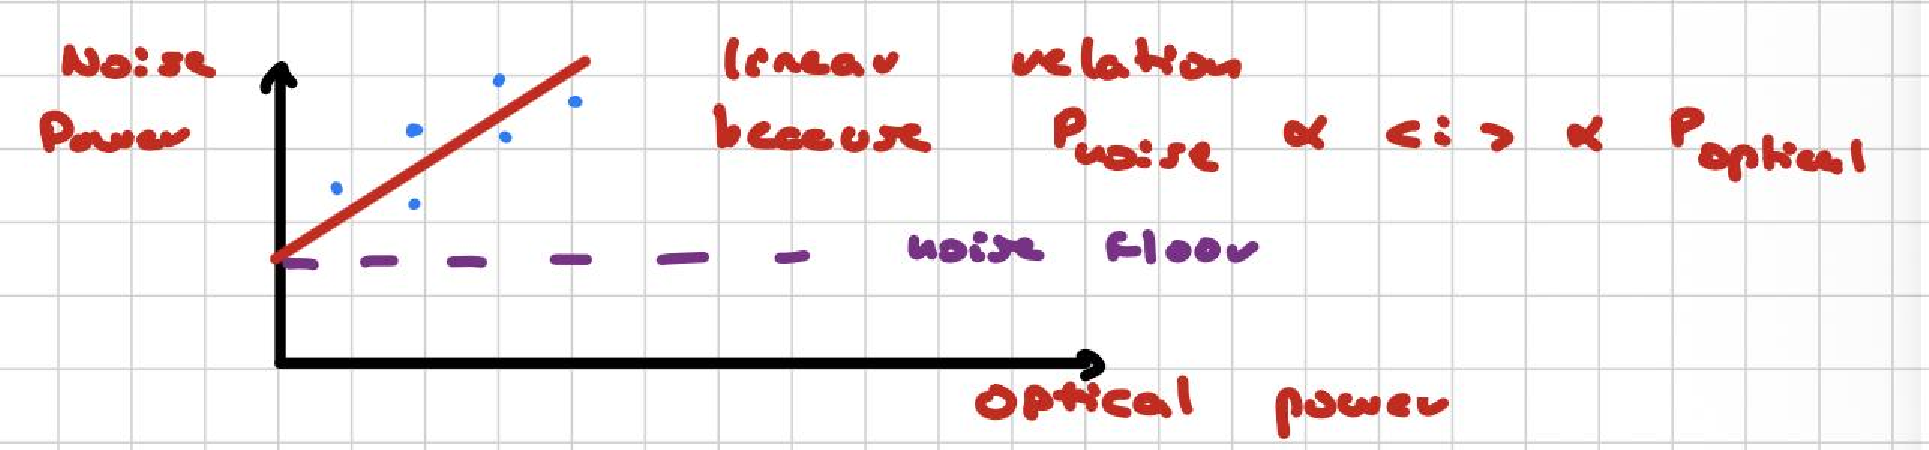
\includegraphics[width=0.8\linewidth]{images_in_pdf/7-/Grafico_35.pdf}
\end{figure}

The \textbf{noise floor} is the background electronic noise of the whole measurement chain, including the amplifier, the load resistor, the cables, and the readout electronics. It is present even in the absence of light and is therefore uncorrelated with the photocurrent. By contrast, \textbf{shot noise} originates from the discrete and random nature of photo-detection events. Even when the average optical intensity is constant, individual photons are detected at random times, and this produces fluctuations in the photocurrent.\\
Shot noise is called \textbf{white} because, within the detector bandwidth, its spectral density is approximately constant as a function of frequency. This does not mean that all physical frequencies contribute equally without limit; rather, it means that the photon-arrival process is essentially delta-correlated on the time scales relevant to the detector. In this sense, shot noise is an intrinsic consequence of the quantized and random character of photo-detection.\\\\
If we want to maximize the \textbf{signal-to-noise ratio} $S/N$, we can modulate the light intensity at a chosen frequency by placing a mechanical chopper in front of the beam. The chopper periodically blocks and transmits the beam, converting a constant (DC) optical signal into a time-dependent (AC) signal at a modulation frequency $f_{\text{mod}}$. 
In this way, the useful signal is shifted from zero frequency to a finite frequency. This does not modify the intrinsic noise sources, but it changes the frequency region in which the measurement is performed. Since technical noise is typically dominant at low frequencies, while shot noise is approximately white within the detector bandwidth, choosing a sufficiently high modulation frequency allows the measurement to be performed in a regime where technical noise is suppressed and the system becomes \textbf{shot-noise limited}.
Therefore, the role of the chopper is not to reduce the noise itself, but to move the signal into a frequency region where the noise is lower and better controlled, improving the overall signal-to-noise ratio.\\\\
Consider now the following setup: a power supply is connected to a laser beam that emits light onto a beam splitter, and one output is reflected onto the detector $D_1$, which is connected to the same power supply.
\begin{figure}[H]
    \centering
    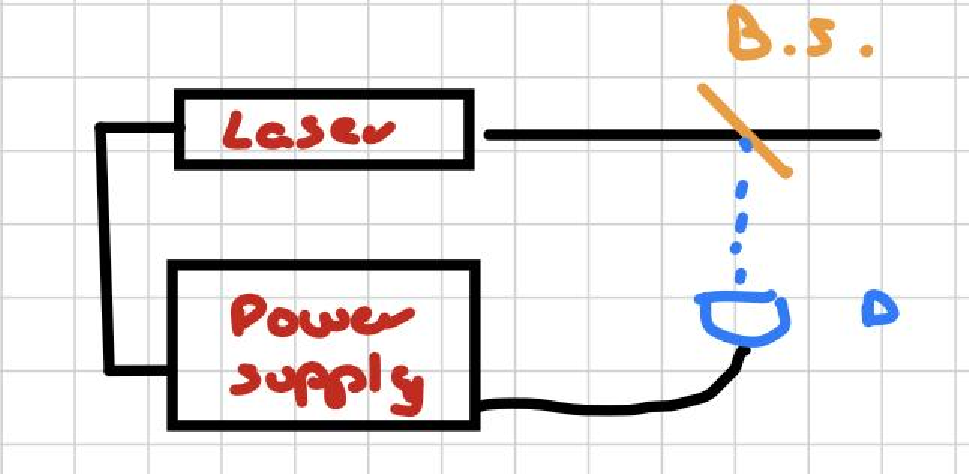
\includegraphics[width=0.8\linewidth]{images_in_pdf/7-/Grafico_36.pdf}
\end{figure}

A small fraction of the laser output is fed back to the power supply. This feedback can reduce classical intensity fluctuations, but it does not modify the fundamental shot-noise contribution.
\begin{figure}[H]
    \centering
    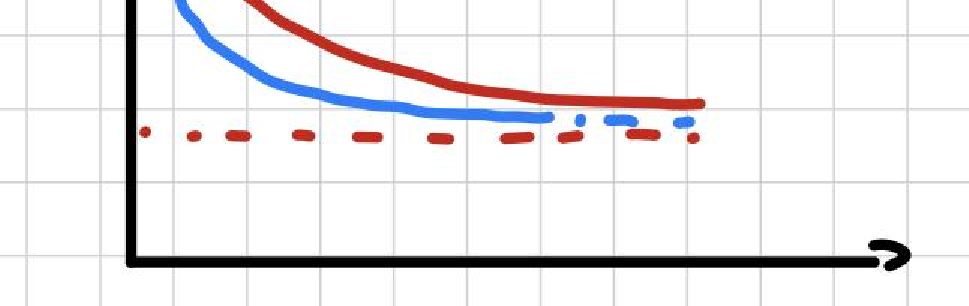
\includegraphics[width=0.8\linewidth]{images_in_pdf/7-/Grafico_37.pdf}
\end{figure}

Suppose instead that a laser beam hits a beam splitter, one part is transmitted to the detector $D_1$ while the other is reflected to detector $D_2$, and the two photocurrents are then combined electronically at a later stage.
\begin{figure}[H]
    \centering
    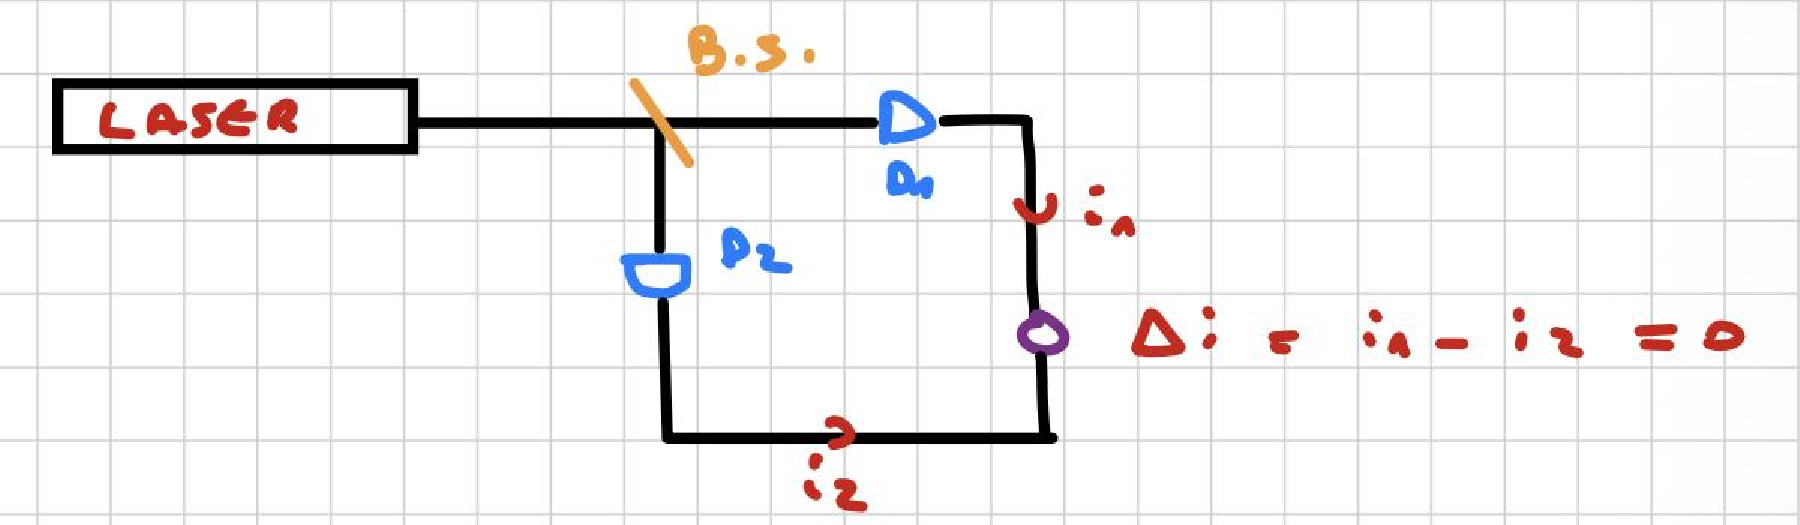
\includegraphics[width=0.8\linewidth]{images_in_pdf/7-/Grafico_38.pdf}
\end{figure}

If there is absorption along one path, the two currents are no longer perfectly equal, so that $\Delta i \neq 0$. This makes it possible to detect very weak variations of light with a better signal-to-noise ratio than with a single detector. This is the idea behind a \textbf{balanced detector}: common-mode technical noise is suppressed by subtraction, while the differential signal survives and can be measured with higher sensitivity.

In this way we can strongly reduce the classical noise component. \textbf{Can we beat the shot-noise limit?} The answer is yes, but only by using nonclassical light sources, such as squeezed states or sub-Poissonian states. In practice, the experimental observation of sub-Poissonian photon statistics also requires detectors with high quantum efficiency $\eta$, because optical losses tend to wash out the nonclassical noise reduction and drive the observed statistics back toward the Poissonian limit.

\section{Photodetectors}\label{sec:photodetectors}
\subsection{Photo-multipliers}
Photomultipliers (PMTs) are based on the external photoelectric effect and on secondary electron emission. A standard PMT is an evacuated glass tube containing a \textbf{photocathode}, a series of \textbf{dynodes}, and an \textbf{anode}.

Electrons emitted by the photocathode are accelerated by a potential difference $\Delta V$ toward the first dynode, where they generate secondary electrons by impact. The typical secondary emission factor is $\delta \approx 3-10$. These electrons are then accelerated to the next dynode, where the process is repeated. After $n$ dynodes, the number of electrons reaching the anode is approximately
\[
G = \delta^n \approx 10^5-10^7 \equiv \text{current amplification or gain}.
\]

In practice, the total gain also depends on the collection efficiency of the electron cascade, but the estimate above captures the main amplification mechanism. The current collected by the anode flows through a load resistor and produces an output voltage signal.
A sufficiently high bias voltage must be applied in order to extract electrons efficiently from the photocathode and accelerate them toward the dynodes.

\subsubsection{PMTs' general properties}
For a photomultiplier we have:
\begin{itemize}
    \item \textbf{Spectral range:} this \hl{indicates the range of wavelengths to which the device is sensitive}. In practice, it depends both on the \textit{photocathode material}, which determines the photoemission threshold, and on the \textit{input window}, which must transmit the incoming light efficiently. A PMT is typically sensitive from the ultraviolet to the visible and, for special photocathodes, up to the near infrared. This quantity is important because it tells us which optical signals can be detected by the device.
    If we study the \textbf{photocathode responsivity}, we observe that for large wavelengths $\lambda$, the photon energy $E = h\nu = hc/\lambda$ becomes too small to eject electrons from the photocathode, so the absorption efficiency drops. As $\lambda$ decreases, the photon energy increases and the responsivity grows, but at sufficiently short wavelengths a cutoff appears. This cutoff is mainly due to the transmission properties of the input window and, in some cases, to the absorption properties of the photocathode material itself. In other words, the spectral response is determined both by the photon energy threshold for photoemission and by the optical transmission of the detector window.
\begin{figure}[H]
    \centering
    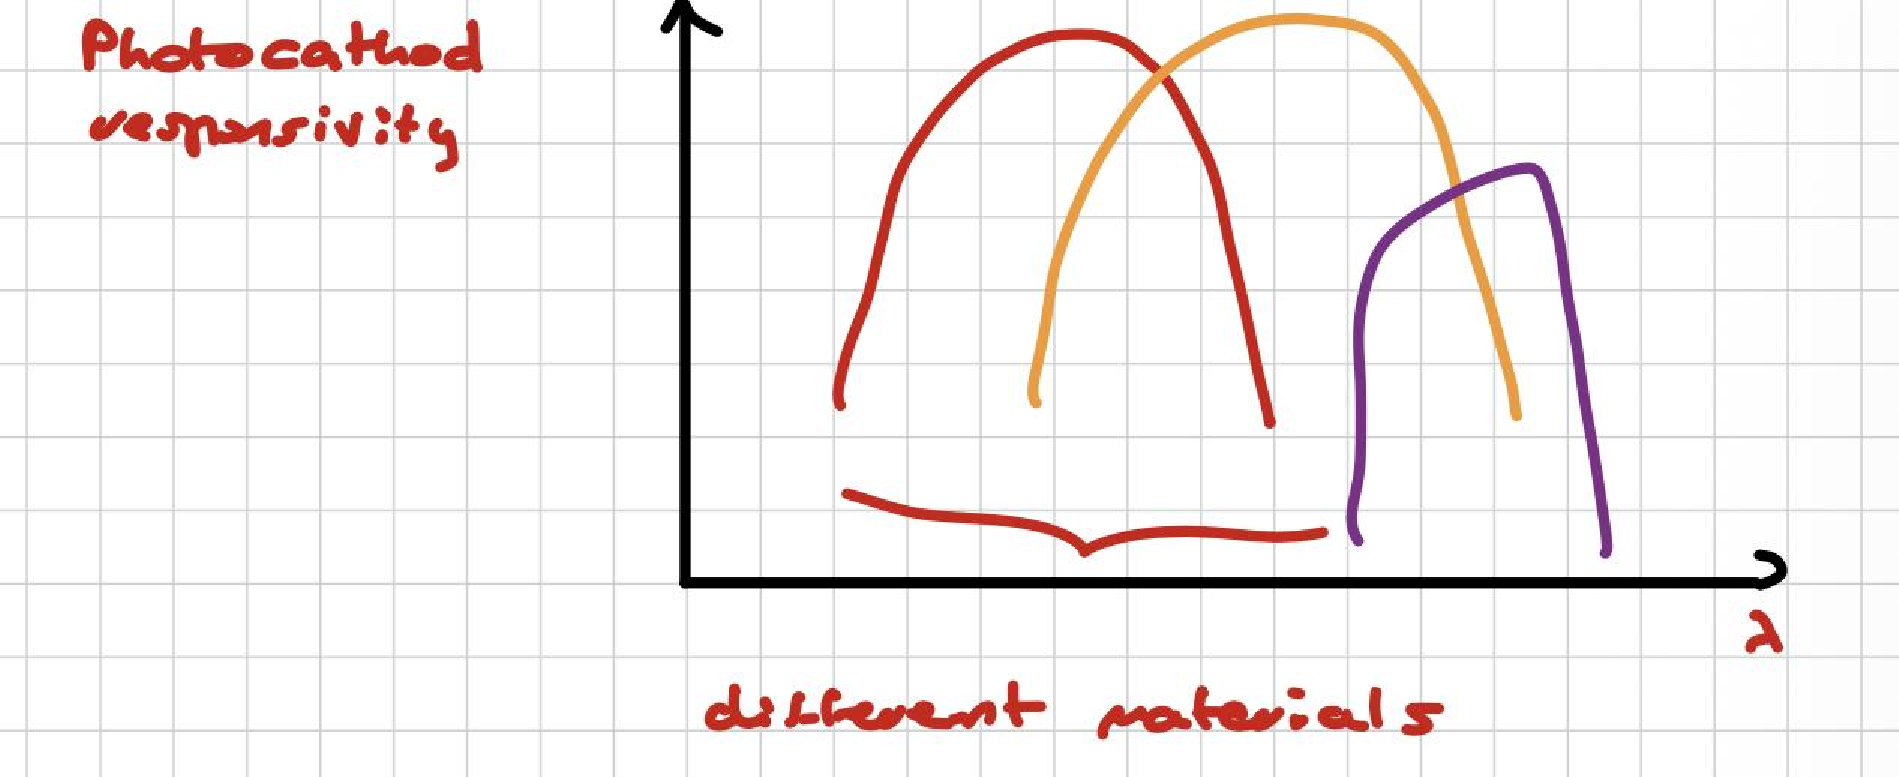
\includegraphics[width=0.8\linewidth]{images_in_pdf/8-/Grafico_39.pdf}
\end{figure}

    \item \textbf{Anode sensitivity:} $K(\lambda)$.
    \begin{equation}\label{eqn:8-photomultiplier-anode-sensitivity}
    \begin{aligned}
    K(\lambda)
    &= \frac{\text{output signal}}{\text{incident radiation power}} =\\[0.5ex]
    &= \frac{S}{\Phi}
    = \frac{S}{I(\mathrm{W/cm^2})\cdot A(\mathrm{cm^2})}
    \hspace{0.4cm}\left[\frac{A}{W}\right]
    \approx 10^3-10^5 \frac{A}{W}.
    \end{aligned}
    \end{equation}

    This quantity measures how efficiently the photomultiplier converts incident optical power into an electrical output signal at a given wavelength. A \hl{larger sensitivity means that a smaller optical power is needed to produce a measurable current}.

    \item \textbf{Quantum efficiency:} $\eta \approx 0.1-50\%$.\\
    The quantum efficiency is the probability that an incoming photon actually produces a photoelectron at the photocathode. It tells us how effective the first step of the detection process is. A higher quantum efficiency means that a larger fraction of the incident photons contribute to the output signal, which is \hl{crucial when measuring weak light}.

    \item \textbf{Maximum anode current:} $\approx 10-100\,\mu A$.\\
    This is the largest current that can be collected at the anode without significantly degrading the performance of the detector. Above this value, heating effects, gain saturation, and possible damage to the device may occur. It sets the upper limit of the dynamic range.

    \item \textbf{Dark current:} $I_d$.\\
    This is the current measured even in complete darkness. It is mainly due to thermionic emission from the photocathode or from the dynodes, and it therefore \hl{increases with temperature}. Since it acts as a false signal, it limits the minimum detectable light level. For this reason, photomultipliers operating in the near infrared are often cooled to reduce dark current.

    \item \textbf{Noise equivalent power:} $\NEP$.\\
    This is the incident optical power that produces an output signal equal to the root-mean-square value of the intrinsic noise of the detector. It is therefore a measure of the weakest detectable optical signal. A smaller $\NEP$ means a more sensitive detector.
    The detected noise increases with the transmission bandwidth $\Delta f$ and scales as $\sqrt{\Delta f}$:
    \begin{equation}\label{eqn:8-photomultiplier-NEP}
    N = K(\lambda)\cdot \NEP \cdot \sqrt{\Delta f}
    \hspace{1cm}
    \NEP = \frac{\sqrt{2e\,I_d\,G}}{K(\lambda)}
    \hspace{0.3cm}\left[\frac{\mathrm{W}}{\sqrt{\mathrm{Hz}}}\right].
    \end{equation}
    
    This expression shows that the $\NEP$ increases when the dark current increases, because the intrinsic noise becomes larger. It also depends on the gain $G$ and on the responsivity $K(\lambda)$.
    The ratio $\frac{S}{N}=1$ when the incident optical power is equal to the $\NEP$; signals weaker than the $\NEP$ are buried in the noise. For $\Delta f \approx 1\,\mathrm{Hz}$, one typically finds $\NEP \approx 10^{-16}-10^{-15}$.

    \item \textbf{Detectivity:} $D = \frac{1}{\NEP}$.\\
    Detectivity is simply the inverse of the $\NEP$. It is useful because a larger detectivity corresponds to a more sensitive detector.

    \item \textbf{Normalized detectivity:} $D^\star$.
    \begin{equation}\label{eqn:8-photomultiplier-normalized-detectivity}
    D^* = \frac{\sqrt{A}}{\NEP} = D\cdot \sqrt{A}
    \hspace{0.4cm}
    \left[\frac{\mathrm{cm}\cdot \sqrt{\mathrm{Hz}}}{\mathrm{W}}\right],
    \end{equation}

    where $A$ is the active area of the device. This quantity is used to compare detectors of different sizes, since it normalizes the detectivity with respect to the detector area.
\end{itemize}


\subsubsection{PMTs' noise sources}
\hl{The total noise of the photomultiplier has several components}, classified as follows:
\begin{enumerate}
    \item \textbf{Shot noise of the photocathode:} the number of detected photoelectrons fluctuates around an average value. For a classical source with Poissonian statistics, the current generated by the detector also fluctuates around its mean value, with rms fluctuations scaling as the square root of the average number of detected events.

    \item \textbf{Excess noise due to secondary electron emission:} the dynode multiplication process is not perfectly deterministic, so the gain itself fluctuates from event to event.

    \item \textbf{Johnson noise in the load resistor:} this is the thermal noise associated with the resistance in the readout circuit.
\end{enumerate}

\calloutwarn{%
Practical downsides of photomultipliers:
\begin{itemize}
    \item They are sensitive, fragile, and expensive.
    
    \item They must be stored in a light-tight box.
    
    \item They require a warm-up time of about $90$ minutes for the operating parameters to stabilize.
    
    \item The bias voltage should not be changed unnecessarily, because it modifies the gain and the response of the device.
    
    \item They require magnetic shielding to protect the electron trajectories from external magnetic fields.
\end{itemize}
}

\subsection{Avalanche photodiodes}
Avalanche photodiodes (APDs) are based on the internal photoelectric effect, i.e. the generation of electron--hole pairs by photon absorption in a semiconductor. These carriers are separated and accelerated by an electric field $\vec{E}$ established across a reverse-biased p--n junction (often in a p-i-n configuration). \calloutinfo{%
Compared to photomultipliers, APDs offer a wider spectral range and a compact solid-state design.
}
The photocarrier multiplication is achieved internally through impact ionization, leading to a gain of $G \approx 10-500$ in linear mode.
\begin{figure}[H]
    \centering
    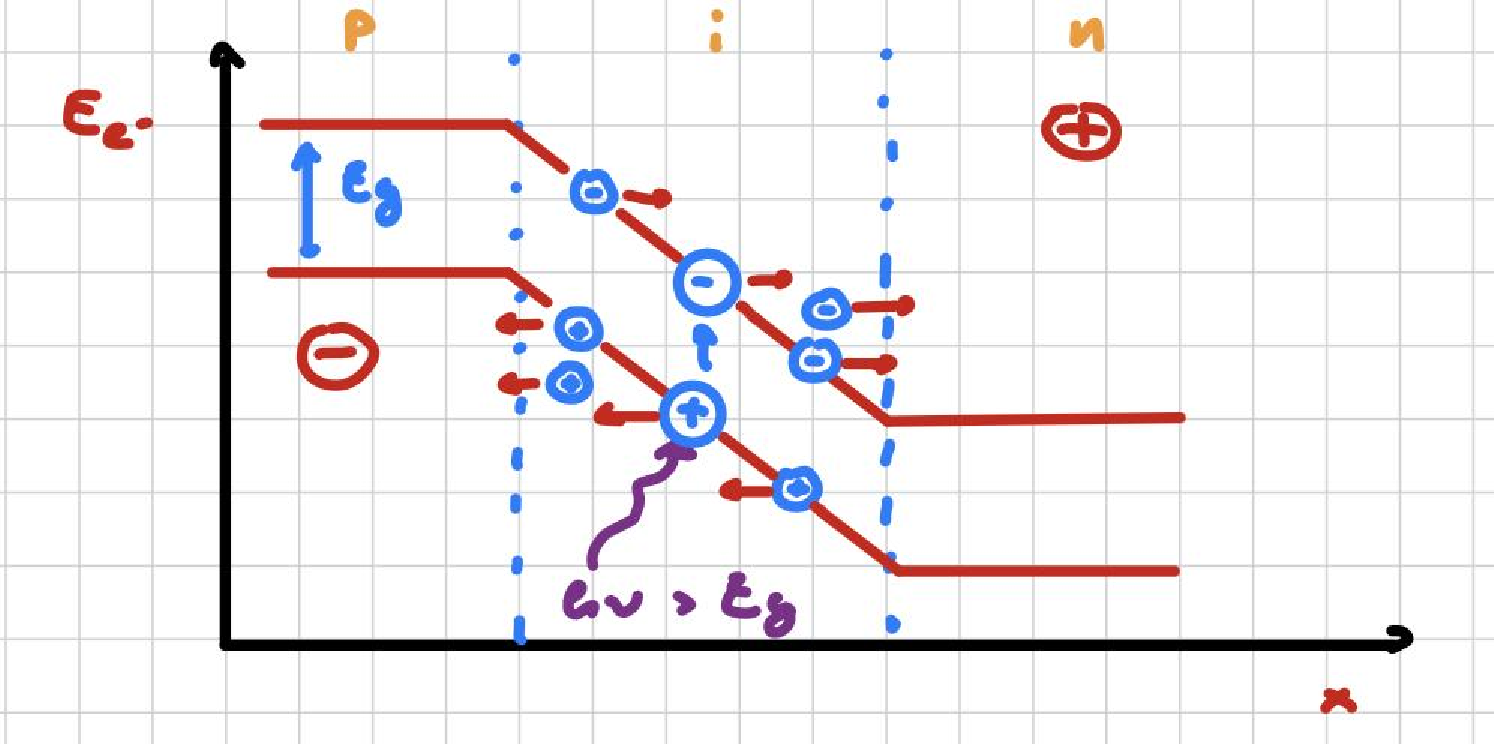
\includegraphics[width=0.8\linewidth]{images_in_pdf/8-/Grafico_40.pdf}
\end{figure}

\subsubsection{APDs' working principle}
\begin{itemize}
    \item A p--n junction is operated under reverse bias, creating a strong electric field in the depletion region.
    \item An incident photon with energy $E = h\nu > E_g$ is absorbed, generating an electron--hole pair.
    \item The electric field $\vec{E}$ accelerates electrons and holes in opposite directions.
    \item If $\vec{E}$ is sufficiently strong, carriers gain enough kinetic energy to ionize atoms by impact, generating additional electron--hole pairs. This leads to an avalanche multiplication process.
\end{itemize}

However, \hl{two main issues arise}:
\begin{enumerate}
    \item \textbf{Carrier multiplication noise and breakdown.}\\
    Both electrons and holes can contribute to impact ionization, which introduces fluctuations in the gain and may lead to uncontrolled avalanche breakdown. To describe this, we define the \textbf{ionization coefficient} $\alpha_i$, i.e. the number of ionization events per unit distance, and the \textbf{ionization ratio}:
    \begin{equation}\label{eqn:8-avalanche-photodiode-ionization-ratio}
    k = \frac{\alpha_h}{\alpha_e}
    \hspace{2ex}
    \begin{cases}
    k \to 0 \Rightarrow \text{electron-dominated multiplication};\\
    k \to \infty \Rightarrow \text{hole-dominated multiplication}.
    \end{cases}
    \end{equation}

    Materials with strongly asymmetric ionization coefficients (small $k$ or large $k$) are preferred, since they reduce the multiplication noise.

    \item \textbf{Trade-off between absorption and electric field.}\\
    A thick intrinsic region improves photon absorption and thus quantum efficiency, while a thin region is required to achieve a strong electric field for avalanche multiplication. This conflict is solved by engineering the device structure, typically separating it into:
    \begin{itemize}
        \item[--] an \textit{absorption layer} (low electric field),
        \item[--] a \textit{multiplication layer} (high electric field).
    \end{itemize}
\end{enumerate}

\subsubsection{APDs' general properties}
\calloutwarn{%
APDs are compact, robust, and less fragile than photomultipliers, but generally exhibit higher noise due to the stochastic nature of the multiplication process.
}
\begin{itemize}
    \item \textbf{Dark noise:}
    \begin{equation}\label{eqn:8-avalanche-photodiode-dark-noise}
    N_{A.P.} = \sqrt{2e\, I_d\, G_{A.P.}^2\, F(G_{A.P.})\, \Delta f}.
    \end{equation}
    Here $G_{A.P.}$ is the avalanche gain, and the factor $G^2$ reflects the amplification of current fluctuations. $F(G)$ is the \textbf{excess noise factor}, which accounts for the statistical nature of impact ionization and depends strongly on the ionization ratio $k$. The dark current $I_d$ includes thermal generation and tunneling contributions.

    \item \textbf{Noise equivalent power:}
    \begin{equation}\label{eqn:8-avalanche-photodiode-NEP}
    \NEP = \frac{\sqrt{2e\, I_d\, G_{A.P.}^2\, F(G_{A.P.})}}{K_{A.P.}(\lambda)}.
    \end{equation}

    This represents the minimum detectable optical power and shows explicitly how the avalanche process increases noise through both $G$ and $F(G)$.

    \item \textbf{Normalized detectivity:}
    \begin{equation}\label{eqn:8-avalanche-photodiode-normalized-detectivity}
    D^* = \frac{\sqrt{A}\, K_{A.P.}(\lambda)}{\sqrt{2e\, I_d\, G_{A.P.}^2\, F(G_{A.P.})}}
    \hspace{0.4cm}
    \left[\frac{\mathrm{cm} \cdot \sqrt{\mathrm{Hz}}}{\mathrm{W}}\right].
    \end{equation}

    For silicon APDs, typical values are $D^* \sim 10^{12}-10^{13}$, significantly lower than photomultipliers, so that:
    \begin{equation}
    \frac{D^*_{P.M.}}{D^*_{A.P.}} \approx 10-100.
    \end{equation}
    
    \item \textbf{Spectral response:} the response typically exhibits a bell-shaped curve.
    \begin{figure}[H]
    \centering
    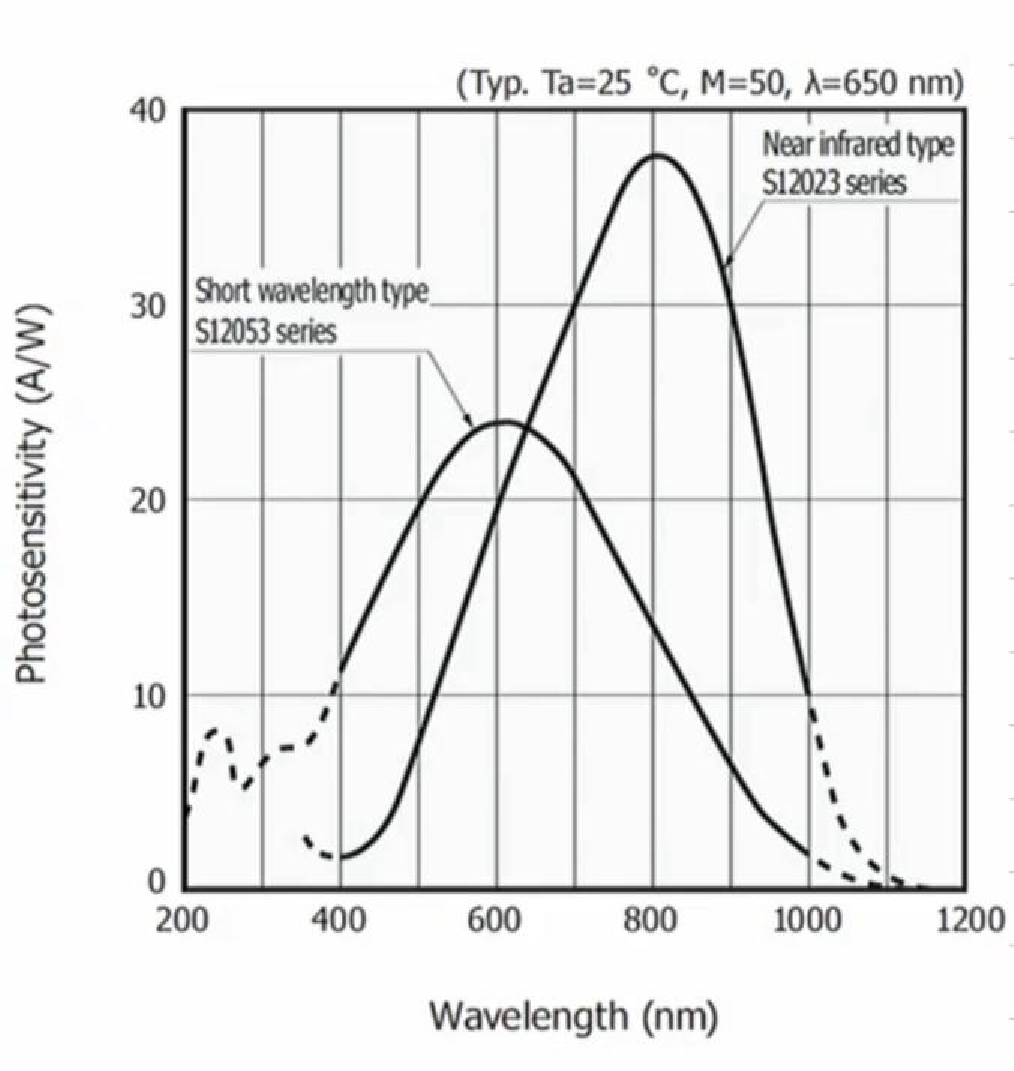
\includegraphics[width=0.4\linewidth]{images_in_pdf/8-/Grafico_41.pdf}
    \end{figure}

    This behavior can be understood as follows:
    \begin{itemize}
        \item For large wavelengths ($\lambda$ high), photon energy is too low ($h\nu < E_g$), so absorption is not possible.
        \item For short wavelengths, the penetration depth is lower and the photons are absorbed very close to the surface, where recombination processes reduce carrier collection efficiency (less multiplication processes).
        \item At intermediate wavelengths, absorption occurs efficiently within the depletion region, maximizing the signal.
    \end{itemize}
\end{itemize}
\subsubsection{APDs' working principle in Geiger mode}
\calloutinfo{%
APDs are also used for very low light detection, including single-photon counting, in the so-called \textbf{Geiger mode}. In this regime, the device is biased above the breakdown voltage, and the gain reaches $G \approx 10^5-10^6$. In this condition, a single absorbed photon can trigger a macroscopic current pulse.
}

\begin{figure}[H]
    \centering
    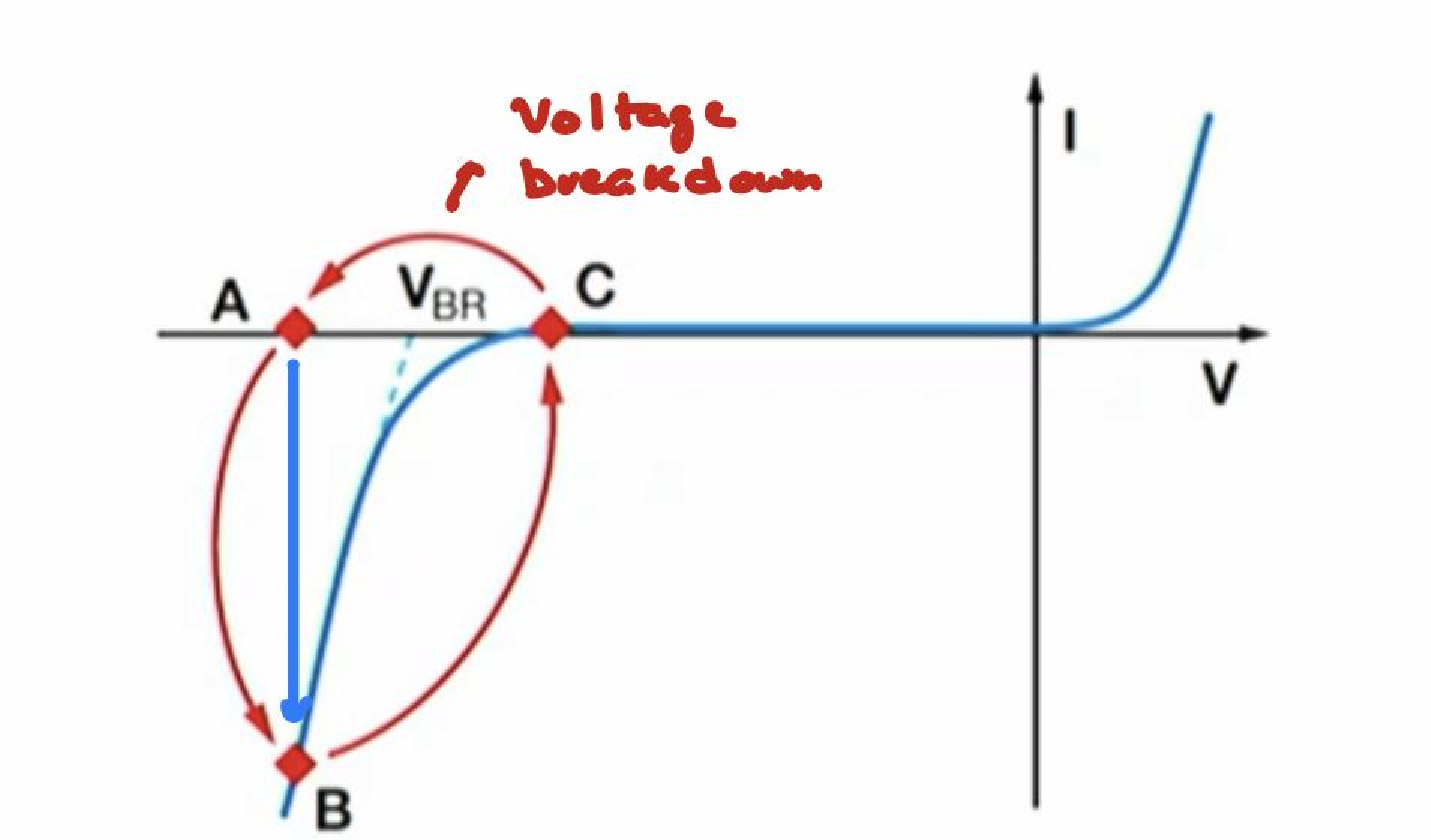
\includegraphics[width=0.6\linewidth]{images_in_pdf/8-/Grafico_42.pdf}
\end{figure}

\begin{enumerate}
    \item The bias voltage is raised to point A, corresponding to a metastable state above breakdown. A single photon absorption can trigger a large avalanche current (point B), producing a detectable pulse.
    
    \item A quenching circuit rapidly lowers the voltage from point B to point C (below the breakdown voltage $V_{BR}$), stopping the avalanche.
    
    \item The voltage is then restored to point A during the so-called \textbf{dead time}, during which the detector is insensitive. In this phase:
    \begin{itemize}
        \item spontaneous avalanches may occur, contributing to the dark count rate;
        
        \item trapped charges in defects may be released later, producing correlated pulses known as \textbf{afterpulses}.
    \end{itemize}
\end{enumerate}
\subsection{Superconducting nanowire single-photon detectors (SNSPDs)}
These detectors are the preferred choice in many landmark experiments and have become a standard tool in quantum communication and quantum computing because of their excellent performance: very high detection efficiency, extremely low dark-count rates, and very short timing jitter. Here, \textbf{time jitter} is the statistical spread of the delay between the arrival of a photon at the detector and the generation of the electrical pulse. A smaller jitter corresponds to a better time resolution.

\subsubsection{SNSPDs' working principle}
\begin{itemize}
    \item The detector must be operated at cryogenic temperature, so that the nanowire remains below the critical temperature $T_C$.
    
    \item When a photon is absorbed by the nanowire, its energy is deposited locally and creates a \textit{hotspot}. This process breaks Cooper pairs and generates quasiparticles.
    
    \item The hotspot locally suppresses superconductivity. If the bias current density becomes larger than the critical current density in that region, i.e. $j > j_c$, a resistive barrier forms.
    
    \item The bias current is then diverted into the external readout circuit, producing a voltage pulse. After a short time, the hotspot cools down and the nanowire returns to the superconducting state.
\end{itemize}
The resistance spike is typically on the order of $\mathrm{k}\Omega$ and is much larger than the input impedance of the readout amplifier, which is typically about $50\,\Omega$. As a consequence, most of the bias current $I_b$ is diverted to the readout circuit, and a measurable voltage pulse is generated.

\begin{figure}[H]
    \centering
    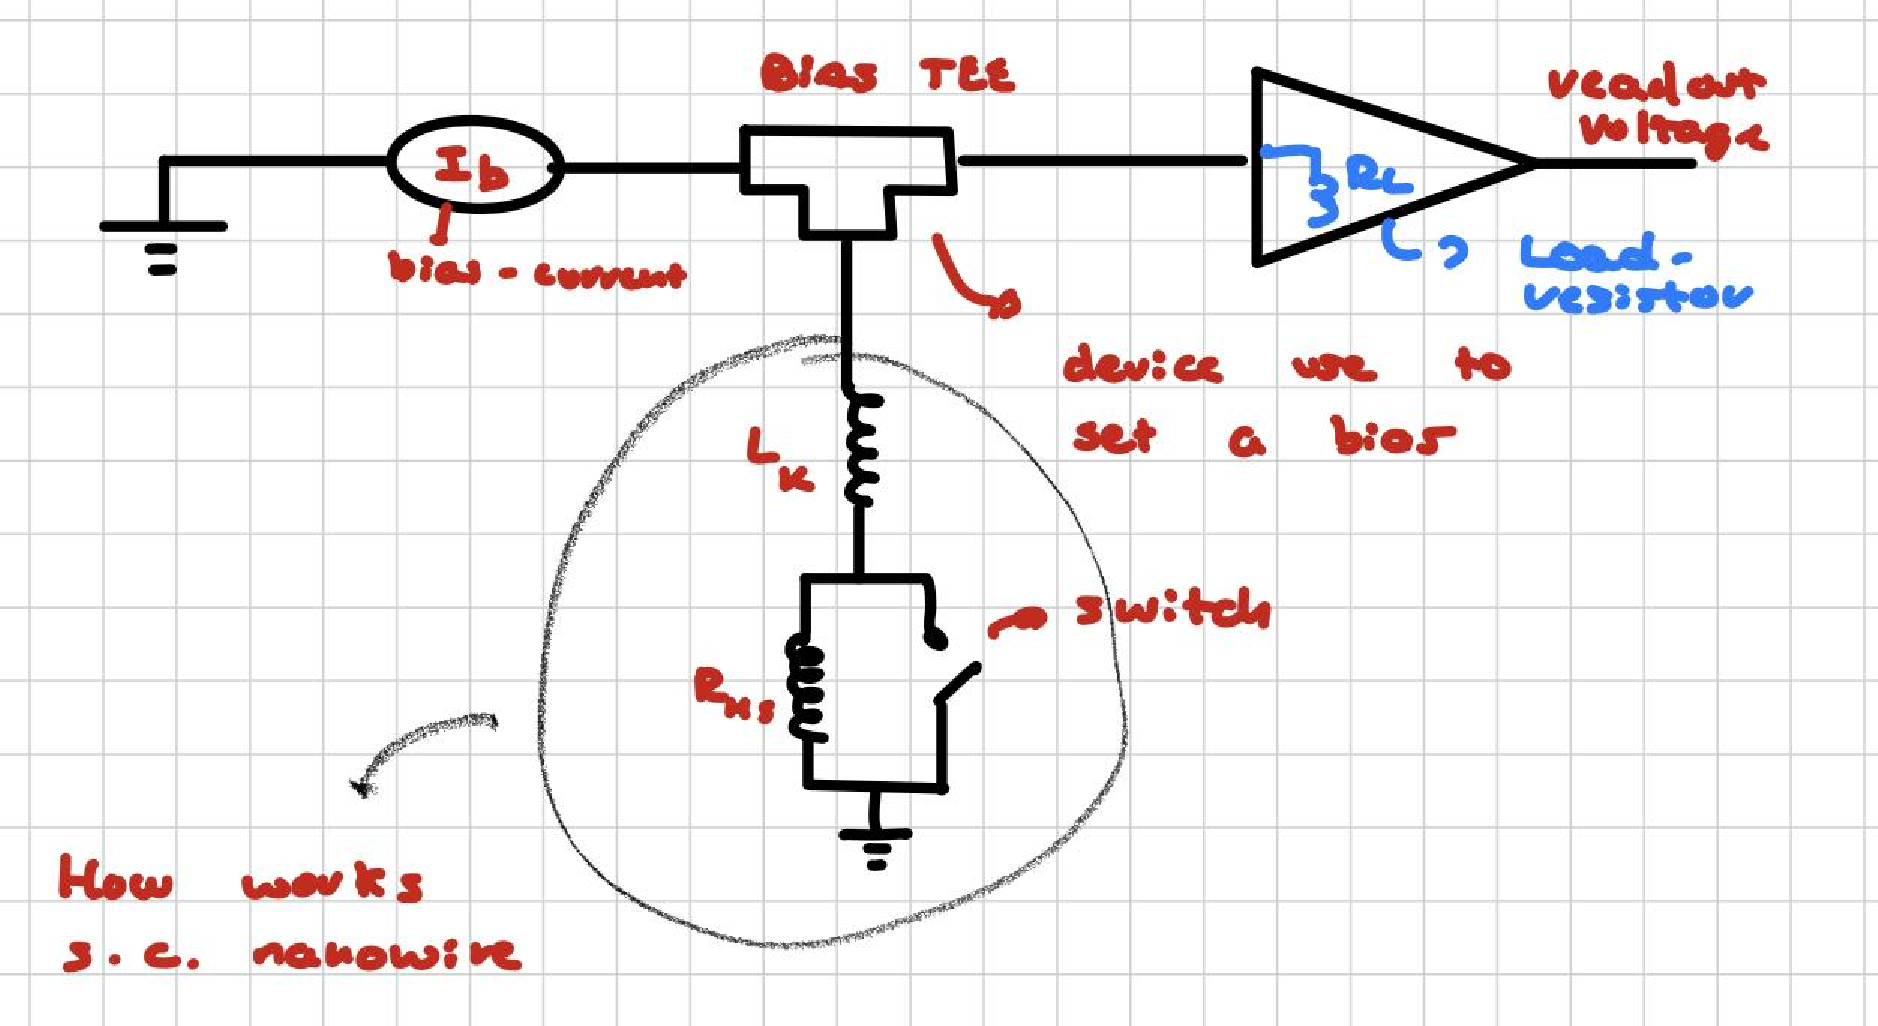
\includegraphics[width=0.8\linewidth]{images_in_pdf/8-/Grafico_43.pdf}
\end{figure}

In the superconducting regime the hotspot resistance satisfies $R_{HS} \approx 0$, while after photon absorption the local resistance becomes finite, $R_{HS} \approx \unit{\kilo\ohm}$, and the current is shunted to the amplifier, producing the output pulse.
\begin{figure}[H]
    \centering
    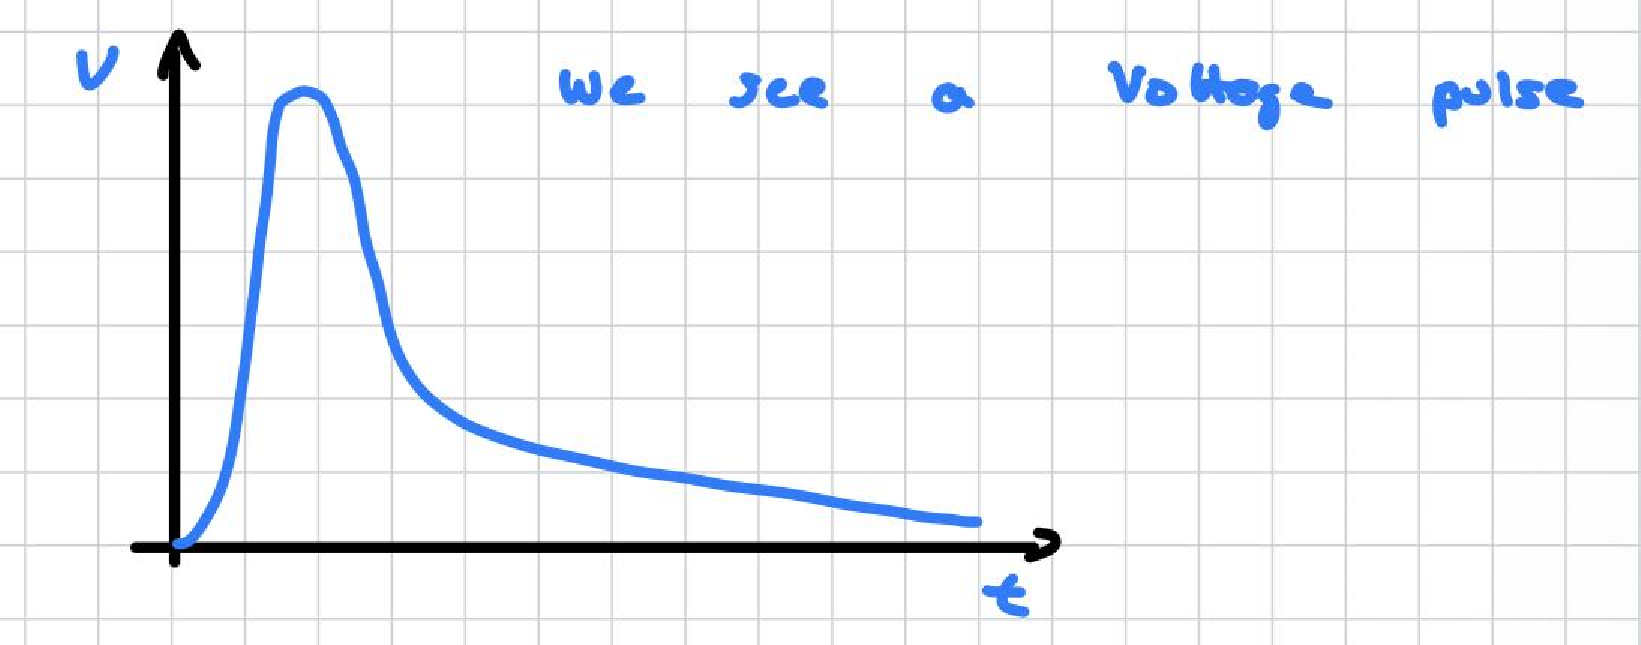
\includegraphics[width=0.8\linewidth]{images_in_pdf/8-/Grafico_44.pdf}
\end{figure}

The current flowing toward the readout circuit is governed by the circuit inductance, and the pulse decay is typically described by a time constant of the form
\[
\tau \sim \frac{L_k}{R_{HS}} \approx \mathrm{ms},
\]
where $L_k$ is the kinetic inductance of the nanowire and $R_{HS}$ is the hot-spot resistance. The recovery of the superconducting state depends on how quickly the hotspot cools down, typically the time constant goes as:
\[\tau \sim \frac{L_k}{R_L}\]
with $R_L \approx \qty{50}{\ohm}$ 

\calloutwarn{%
If the resistive region does not cool sufficiently fast, the detector can enter a \textbf{latching} regime, in which it remains trapped in a resistive state and cannot detect new photons.
}

\subsubsection{SNSPDs' fabrication and spectral response}

Different superconducting materials can be used, each with its own critical temperature and energy gap. The fabrication typically proceeds as follows:
\begin{itemize}
    \item A dielectric layer is deposited on a silicon wafer together with an optical cavity, usually designed as a quarter-wave structure, and a thin superconducting film. The optical cavity maximizes the absorption probability in the superconducting layer.
    \item Electron-beam lithography is then used to pattern the superconducting film into a nanowire and to define the electrical contacts.
    \item After the electrical contacts are fabricated, optical coupling is realized by aligning an optical fiber precisely above the nanowire, which requires a very high coupling efficiency.
    \item The final device is compact, robust, and highly sensitive, but it must be operated with dedicated cryogenic equipment.
\end{itemize}
The superconducting energy gap sets a limit on the detectable wavelength. In practice, one can identify different wavelength windows, and the optical cavity can be engineered to maximize absorption in the desired spectral region.
\begin{figure}[H]
    \centering
    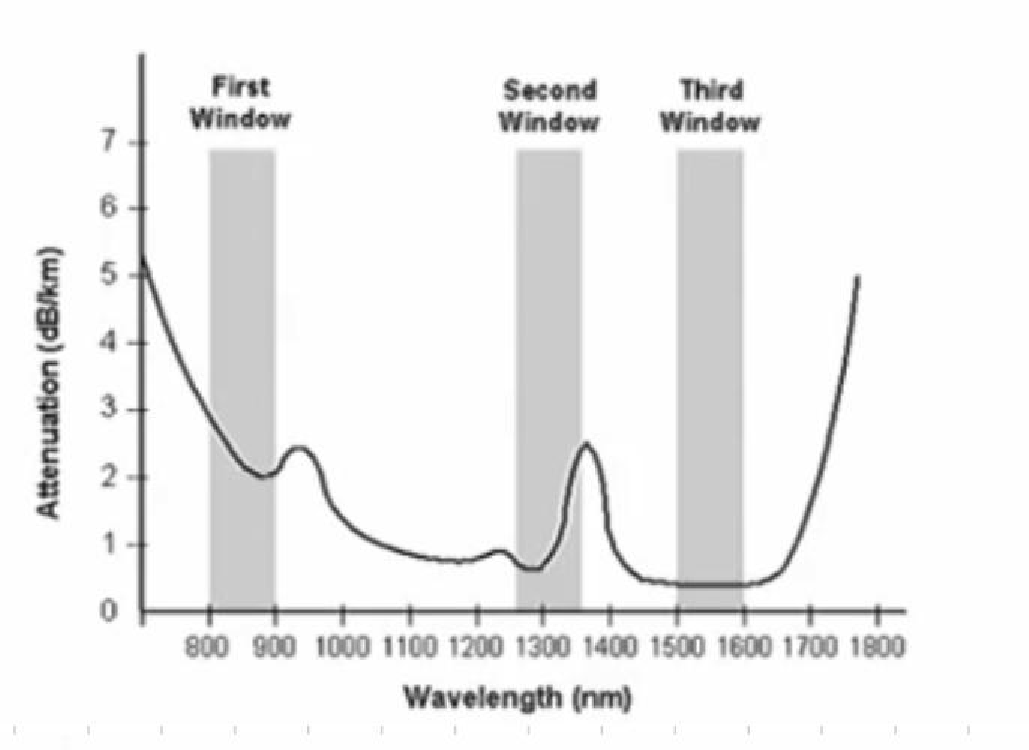
\includegraphics[width=0.8\linewidth]{images_in_pdf/8-/Grafico_45.pdf}
\end{figure}

\begin{figure}[H]
    \centering
    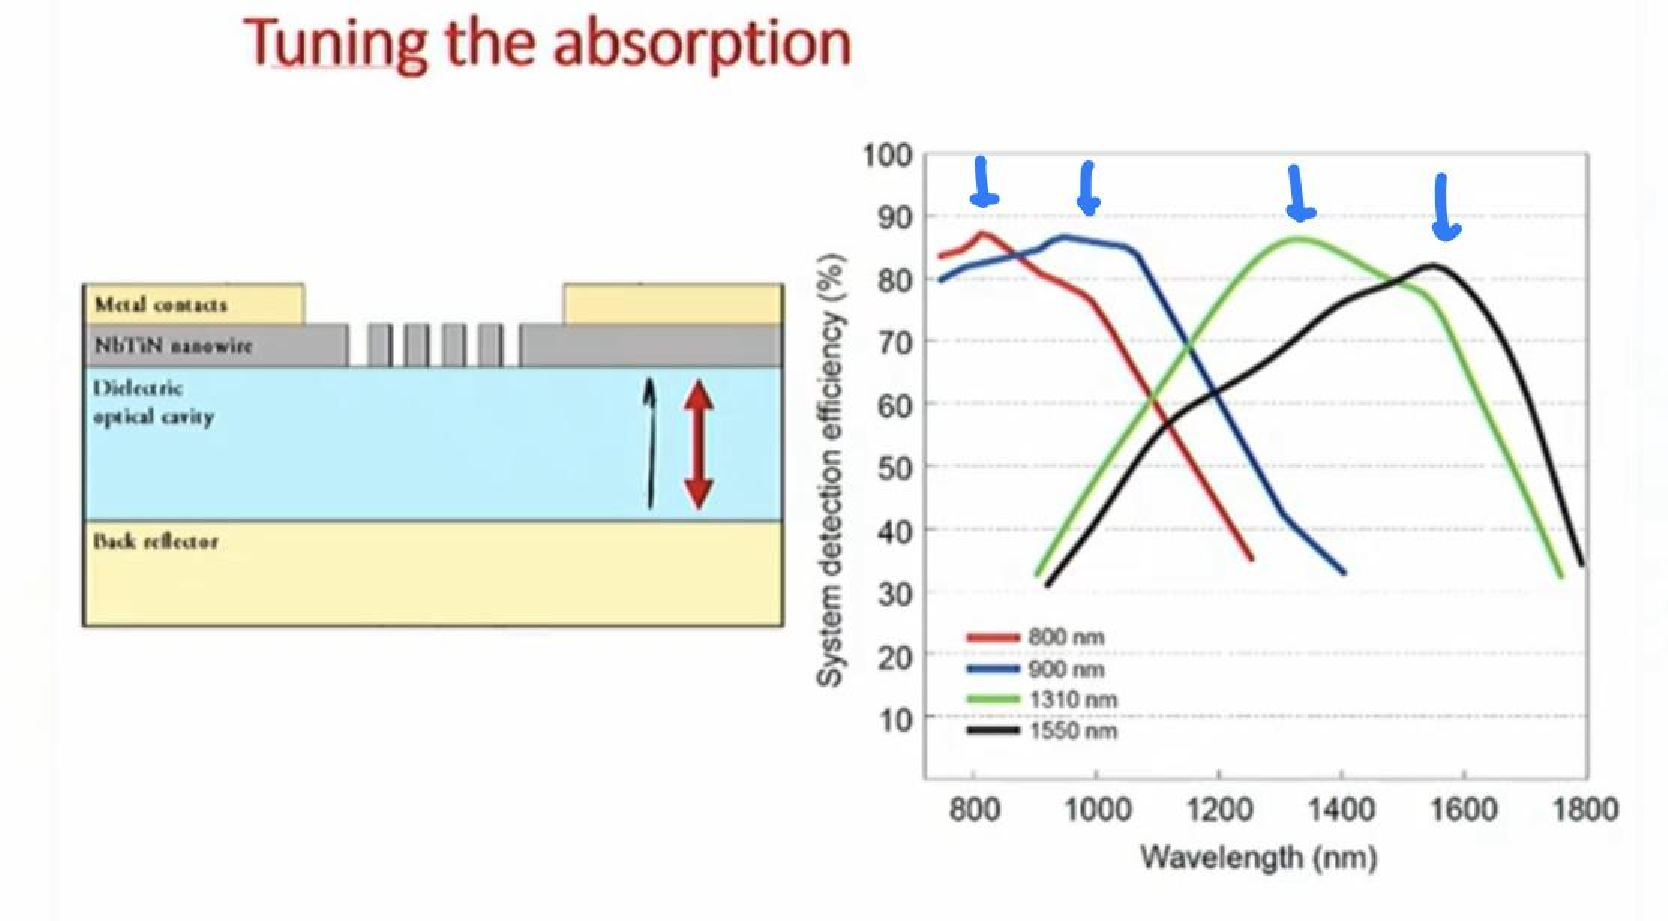
\includegraphics[width=0.8\linewidth]{images_in_pdf/8-/Grafico_46.pdf}
\end{figure}

When $\lambda$ is in the infrared range, the dark-count rate increases because blackbody radiation from the room and the surrounding environment can be coupled into the fiber and reach the detector.
The absorption also depends on the polarization of the incoming light:
\begin{figure}[H]
    \centering
    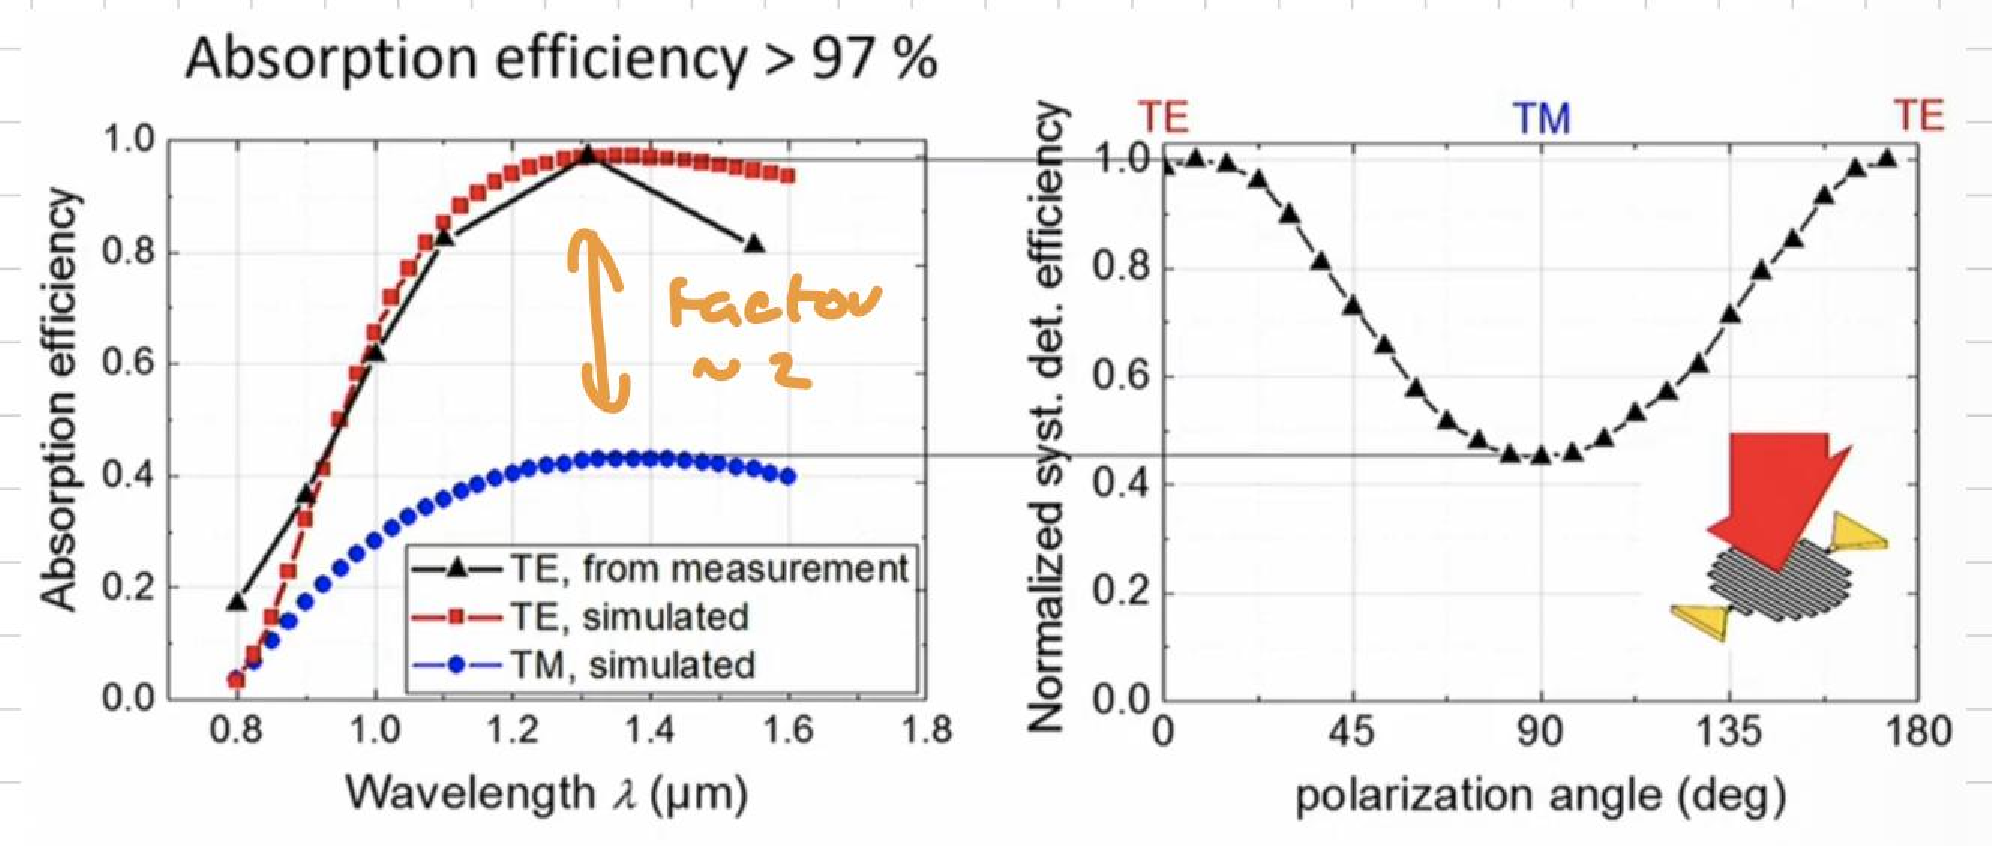
\includegraphics[width=0.8\linewidth]{images_in_pdf/8-/Grafico_47.pdf}
\end{figure}

The detector response can be different for \textbf{TE} (transverse electric) and \textbf{TM} (transverse magnetic) polarization, so the polarization must be taken into account carefully because it can strongly affect the absorption efficiency.
The time jitter depends on both electrical noise and geometry. Since the signal propagates through the detector with a finite speed, photons absorbed at different positions can produce pulses that arrive at slightly different times. The timing jitter is usually quantified by the full width at half maximum (FWHM) of the arrival-time distribution. For a Gaussian distribution, the FWHM is related to the standard deviation by
\[
\mathrm{FWHM} = 2\sqrt{2\ln 2}\,\sigma,
\]
and in optimized SNSPDs it can reach values of the order of a few picoseconds.

\section{Photon counting}\label{sec:photon-counting}
We have already seen that the absorption of a single photon can generate a pulse in a photodetector. We can define the number of pulses per unit time, $N_r$, and the number of photons impinging on the detector per unit time, $N_p$. In general,
\[
N_r \leq N_p,
\]
because the detector quantum efficiency is smaller than or equal to one. In the linear regime, more precisely, one has
\[
N_r \simeq \eta\,N_p,
\]

where $\eta$ is the overall detection efficiency of the system.
\textbf{How do we count photons?}
\begin{itemize}
    \item The output signal consists of single voltage spikes superimposed on low- and high-frequency noise. These spikes correspond to individual detection events.
    \item The signal is fed into an amplifier, typically with a large gain, and low-frequency ripples are filtered out. This step improves the visibility of the real pulses with respect to the electronic background.
    \item The signal then enters a discriminator, which rejects pulses below a chosen threshold. In this way, pulses due to thermionic emission or other spurious effects can be removed.
    \item The accepted pulses are sent to a pulse shaper and then converted into a standard \textbf{TTL} (transistor-transistor logic) signal at the output.
    \item These TTL pulses are counted by an electronic counter and stored as digital information, namely as the number of pulses per unit time. If an analog output is needed, a digital-to-analog converter can be used.
\end{itemize}
For photon counting it is preferable to have:
\begin{enumerate}
    \item A short temporal width of the output pulse, so that individual events can be clearly separated from one another and from spurious pulses. Shorter pulses allow higher count rates, typically on the order of $10-20\,\mathrm{ns}$.
    \item A high quantum efficiency $\eta$ of the photocathode and a low anode dark current. This is essential to maximize the signal-to-noise ratio, since a high number of primary photoelectrons must be generated while thermally induced electrons must be minimized.
    \item An appropriate pulse-height distribution. The pulse heights corresponding to true signal events and to dark counts may overlap only partially, and in general the average amplitude of signal pulses is expected to be higher than that of dark pulses. 
    \begin{figure}[H]
        \centering
        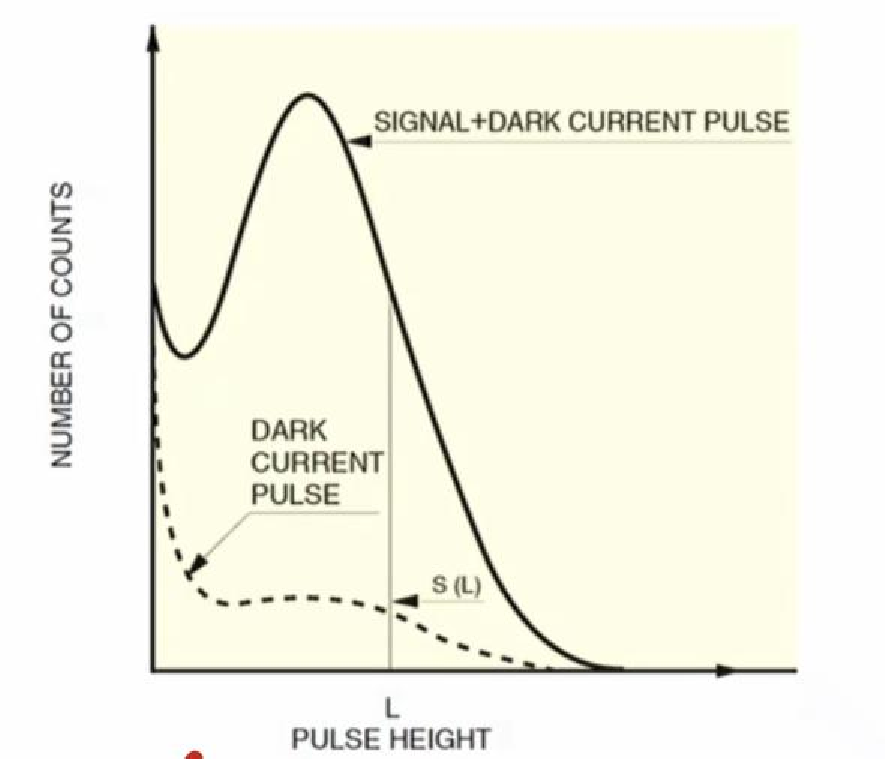
\includegraphics[width=0.4\linewidth]{images_in_pdf/9-/Grafico_48.pdf}
        \caption{Histogram of the occurrence of pulses with height $L$.}
    \end{figure}

    \item A careful choice of the photomultiplier voltage and of the discrimination threshold. If the count rate is measured as a function of the supply voltage, the signal typically increases faster than the noise at sufficiently high voltages. This happens because the discriminator suppresses a large fraction of the dark counts; only after the threshold voltage $V_0$ is reached does the signal-to-noise ratio saturate and approach a plateau.
    \begin{figure}[H]
        \centering
        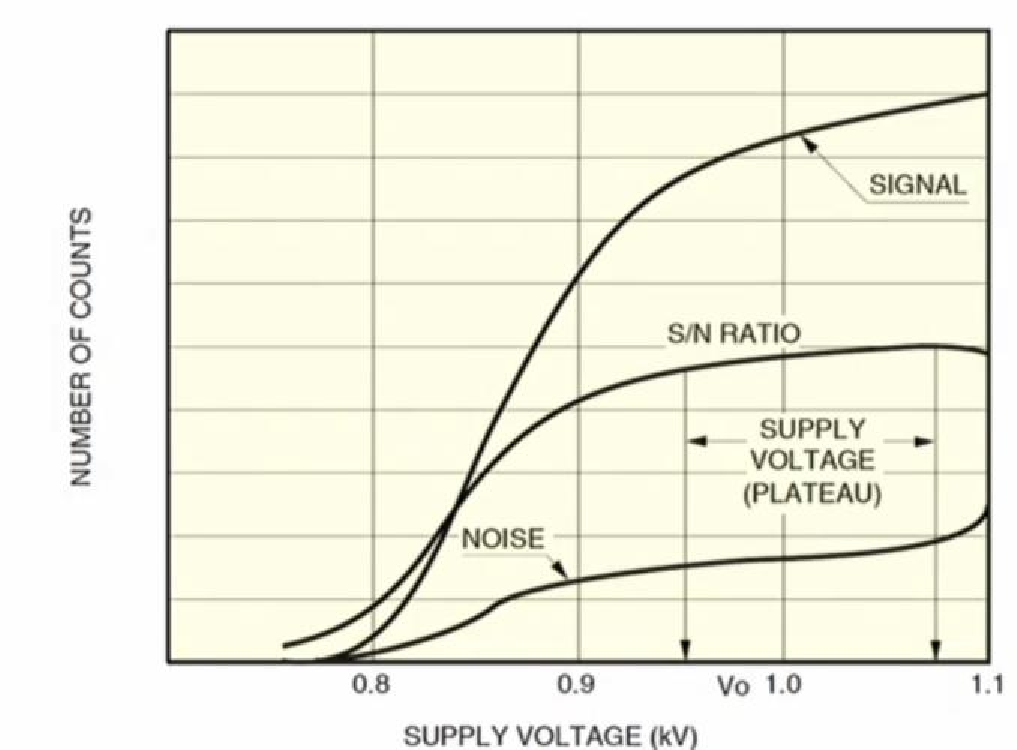
\includegraphics[width=0.4\linewidth]{images_in_pdf/9-/Grafico_49.pdf}
    \end{figure}

\end{enumerate}

\subsection{Time-correlated photon counting}
Time-correlated photon counting is a technique based on the statistics of light emission following excitation by a short light pulse. After excitation, the luminescence signal builds up and then decays in time. The detector records the arrival times of single photons, that is, the times at which individual pulses appear at the output. Each pulse corresponds to a single photoelectron emitted at the photocathode.

\textbf{How does it work?}
\begin{enumerate}
    \item We define $t=0$ as the time when the excitation pulse is emitted.
    \item The excitation pulse is repeated many times, so that the luminescence process is observed over a large number of identical cycles. The goal is to reconstruct the temporal decay of the emitted light by building a histogram of the photon arrival times within time intervals $\Delta t$.
    \begin{figure}[H]
        \centering
        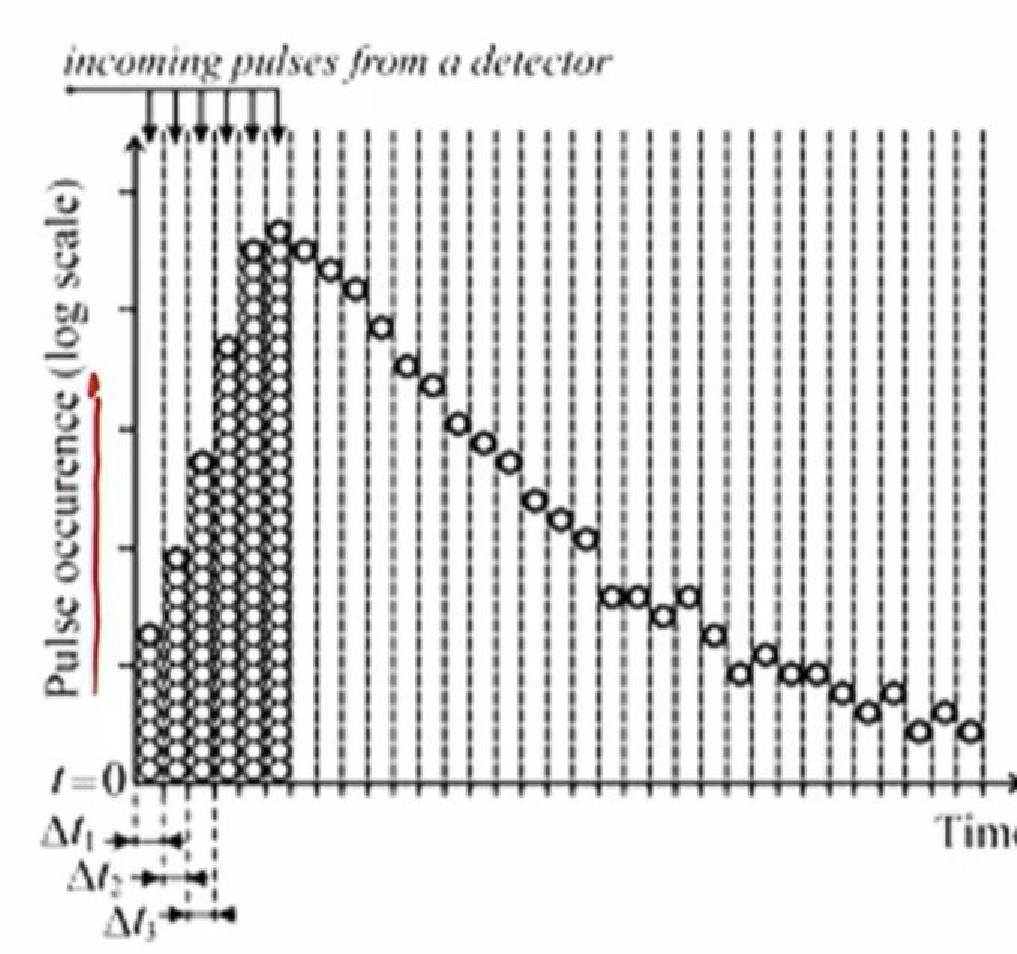
\includegraphics[width=0.4\linewidth]{images_in_pdf/9-/Grafico_50.pdf}
    \end{figure}

    The probability of detecting a photon at a given time is proportional to the number of fluorescence centers still in the excited state. As the experiment is repeated many times, the detection events are randomly distributed among the available time bins, and the accumulated histogram reproduces the decay law of the luminescence.
    
    To obtain reliable statistics, some conditions are required:
    \begin{itemize}
        \item The excitation intensity must be low enough to ensure that, on average, only one photon is detected per cycle, or at least that the probability of multiple detections per pulse remains small.
        \item A large number of events must be accumulated, so high repetition-rate lasers, typically in the kHz--MHz range, are used.
        \item A time-to-amplitude converter is employed. At $t=0$ the excitation pulse starts a linear voltage ramp; when the stop pulse arrives from the detector, the ramp is interrupted. The final voltage is proportional to the delay between the start and stop signals.
        This voltage is then sorted according to its amplitude and assigned to the corresponding channel of a multichannel analyzer. In this way, the number of events in each channel gives a histogram that is proportional to the photon arrival-time distribution, from which the characteristic lifetime can be extracted.
        \begin{figure}[H]
            \centering
            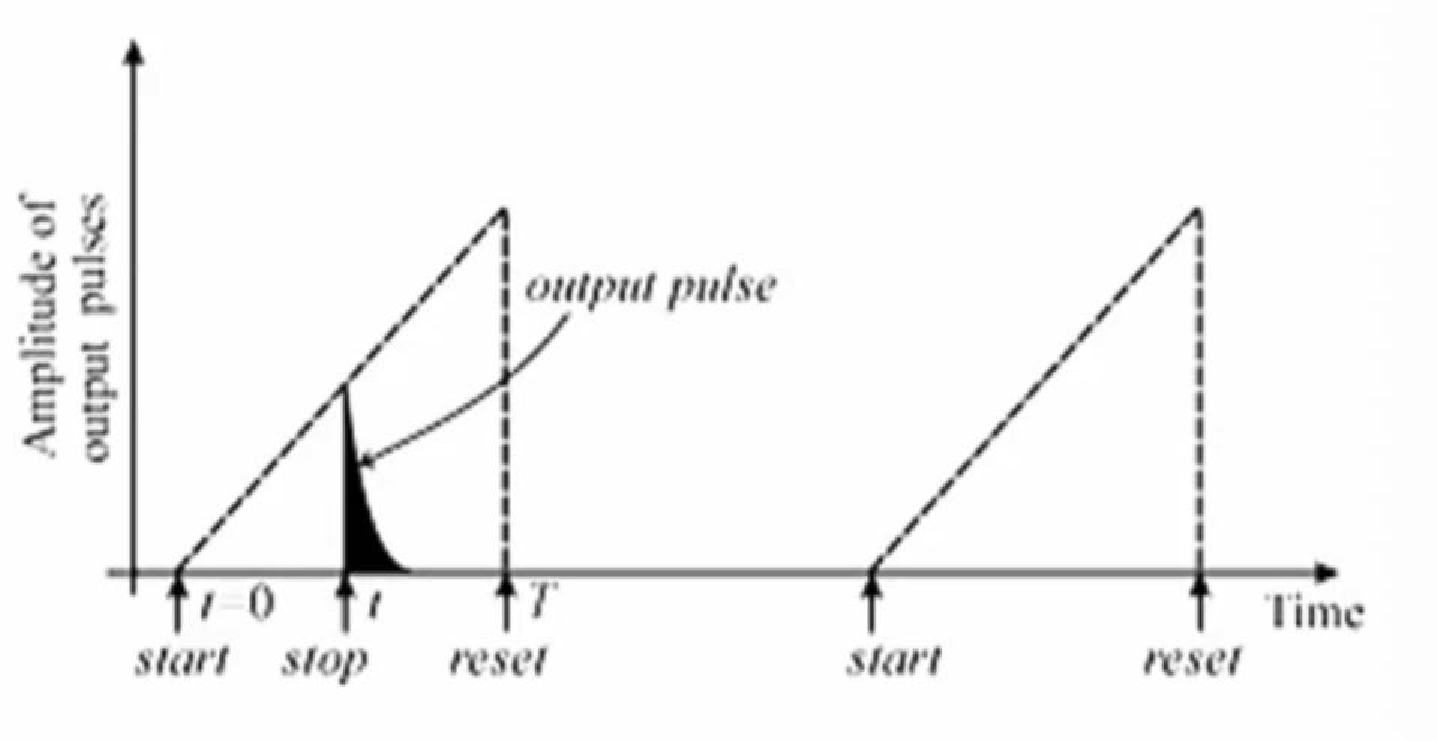
\includegraphics[width=0.4\linewidth]{images_in_pdf/9-/Grafico_51.pdf}
        \end{figure}

    \end{itemize}
\end{enumerate}

\section{Photon Antibunching}\label{sec:photon-antibunching}
Remember that light can be classified according to its photon statistics. We have already used Young's experiment and the Mach--Zehnder interferometer to introduce the concept of first-order coherence (Eqn.~\ref{eqn:6-degree-of-first-order-coherence}):
\begin{equation}
g^{(1)}(\tau)=\frac{\langle E^*(t)\,E(t+\tau)\rangle}{\langle E^*(t)\,E(t)\rangle},
\end{equation}

which is useful for determining how monochromatic a source is and for estimating the coherence time or coherence length of the light. However, \hl{first-order coherence does not contain information about the actual statistical properties of the light field}. That information is carried by the \textbf{intensity fluctuations}.

Suppose that we perform two-time measurements in which many pairs of intensity readings are taken with a fixed time delay $\tau$. The average of the product of each pair of readings defines the \textbf{intensity correlation function}, which is the intensity analogue of the first-order field correlation function.

We are interested in measuring the coincidence rate:
\[
C(t,t+\tau)=\langle I(t)\,I(t+\tau)\rangle,
\]

where the two intensities are detected by two different detectors.

If the field is stationary, the average depends only on the time delay, so we can define the \textbf{second-order correlation function} as
\begin{equation}\label{eqn:10-second-order-correlation-function}
g^{(2)}(\tau)=
\frac{\langle I(t)\,I(t+\tau)\rangle}{\langle I(t)\rangle^2} =
\frac{\langle E^*(t)E^*(t+\tau)E(t)E(t+\tau)\rangle}{\langle E^*(t)E(t)\rangle^2}.
\end{equation}

For a classical stationary field, the normalized first-order correlation satisfies
\[
|g^{(1)}(\tau)|\le 1.
\]

If the intensity is constant, $I(t)=I(t+\tau)=I_0$, then
\[
g^{(2)}(\tau)=1.
\]

When $\tau = 0 \implies g^{(2)}(0) = \frac{\braket{I(t)^2}}{\braket{I(t)}^2}$ and for a sequence of N measurements taken at times $t_1,t_2,...t_N$ the averages are given by:
\[\braket{I(t)} = \frac{I(t_1)+...+I(t_N)}{N}\hspace{1cm}\braket{I(t)^2} = \frac{I^2(t_1)+...+I^2(t_N)}{N}\]

But according to \textbf{Cauchy inequality}: 
\begin{equation}\label{eqn:cauchy-inequality}
2\cdot I(t_1)\cdot I(t_2) \leq I^2(t_1)+I^2(t_2)
\end{equation}

it applies to any pair of time $t_i$ and hence to all cross terms in $\braket{I^2(t)}$, we obtain:
\[\braket{I^2(t)} \geq \braket{I(t)}^2 \implies g^{(2)}(0) = \frac{\braket{I(t)^2}}{\braket{I(t)}^2}\geq 1 \]

There is no way to establish an upper limit, so the allowed values are:
\[1 \leq g^{(2)}(0) < +\infty\]

For not-zero time delays, the positive nature of the intensity guarantees that:
\[0 \leq g^{(2)}(\tau) < +\infty\]

We can also obtain another result using the Cauchy inequality:
\begin{equation}\label{eqn:cauchy-inequality-2}
[I(t_1) I(t_1+\tau) + \dots + I(t_N) I(t_N+\tau)]^2 \leq 
\left[
    [I^2(t_1) + \dots + I^2(t_N)] [I^2(t_1+\tau) + \dots + I^2(t_N+\tau)]
\right]
\end{equation}

For a long series of measurements, the two series on the right hand side are equivalent and the square root of the previous equation leads to:
\[\braket{I(t) \cdot I(t+\tau)} \leq \braket{I(t)}^2\]
\[\implies g^{(2)}(\tau) = \frac{\braket{I(t)\cdot I(t+\tau)}}{\braket{I(t)}^2} \leq 1 \leq g^{(2)}(0) \]

\calloutinfo{%
So we obtain the \textbf{limits for classical light fields}:
\begin{equation}\label{eqn:10-classical-light-second-order-correlation}
g^{(2)}(\tau) < g^{(2)}(0) \hspace{1ex} \land \hspace{1ex}
1 \leq g^{(2)}(0) < +\infty, \hspace{1ex} \forall\tau \ne 0
\end{equation}

This means that, within classical optics, the \textbf{zero-delay correlation is the largest one}. A violation of this condition is a signature of quantum light.
}

We can now consider some important cases:
\begin{enumerate}
    \item \hl{For a perfectly coherent light field},
    \begin{equation}\label{eqn:10-coherent-light-second-order-correlation}
    g^{(2)}(\tau)=1 \qquad \forall\,\tau.
    \end{equation}
    This is the expected result for an ideal laser-like source with Poissonian photon statistics.

    \item \hl{For a light source made of a large number of independent emitters}, undergoing collisions and \emph{Doppler broadening}, the field is \emph{chaotic} and gaussian distributed. In this case the \textbf{Siegert relation} holds:
    \begin{equation}\label{eqn:10-siegert-relation}
    g^{(2)}(\tau)=1+|g^{(1)}(\tau)|^2
    \end{equation}

    and since
    \[
    0\le |g^{(1)}(\tau)|\le 1,
    \]

    one has
    \begin{equation}\label{eqn:10-chaotic-light-second-order-correlation}
    1\le g^{(2)}(\tau)\le 2.
    \end{equation}

    This is the typical bunching behavior of thermal light.

    \item \hl{For a source with a Lorentzian spectral profile}, such as a collision-broadened source,
    \[
    g^{(2)}(\tau)=1+e^{-2|\tau|/\tau_c},
    \]

    so that
    \[
    g^{(2)}(\tau)\to 1 \qquad \text{for } |\tau|\to\infty,
    \]

    and
    \[
    g^{(2)}(0)\to 2.
    \]
\end{enumerate}
\begin{figure}[H]
    \centering
    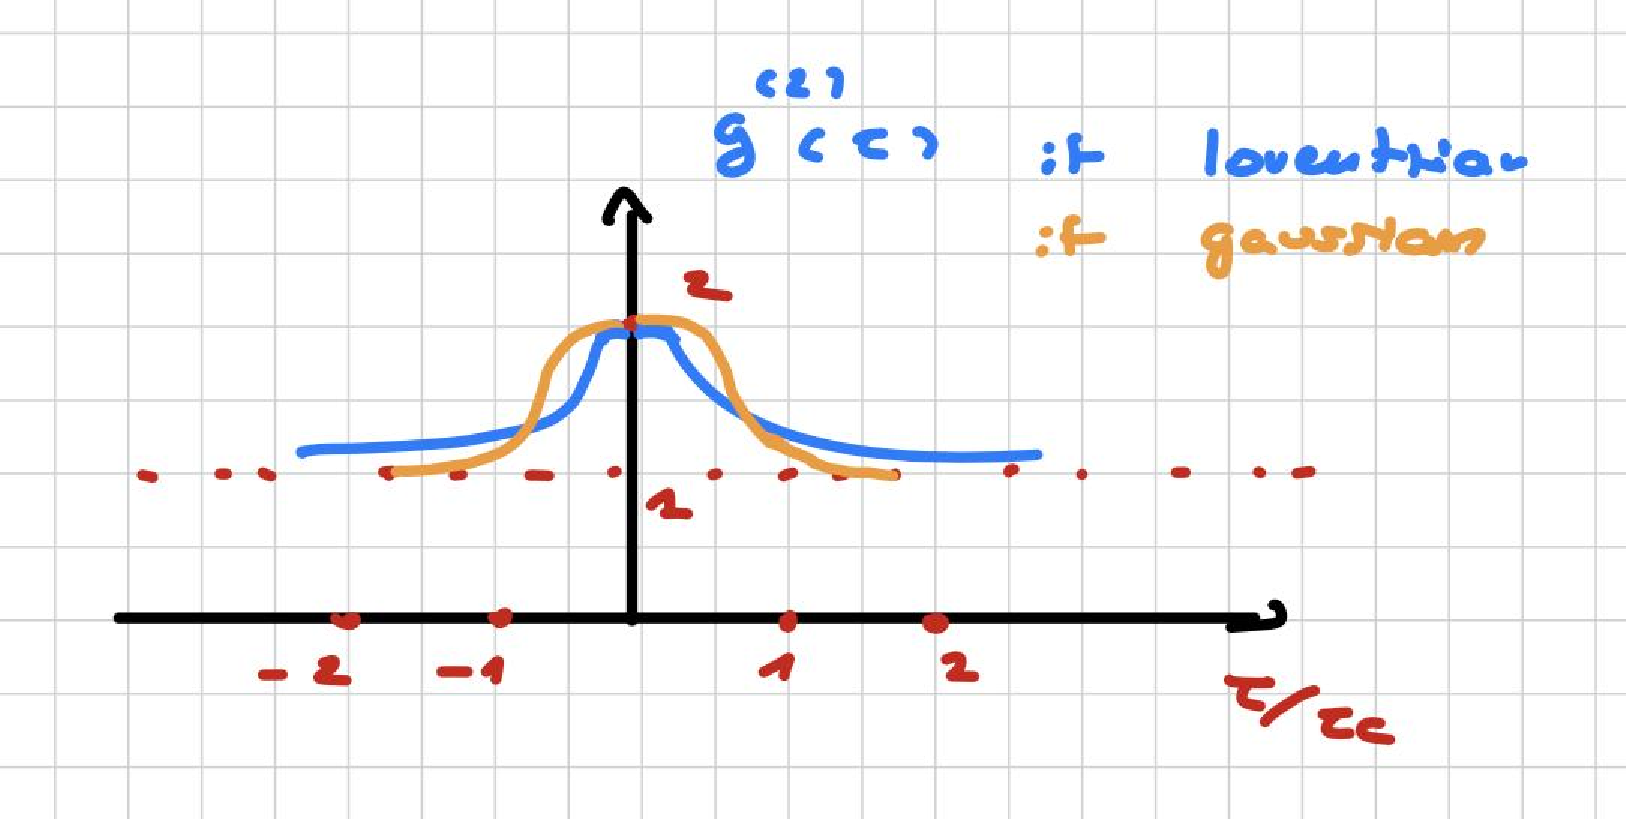
\includegraphics[width=0.6\linewidth]{images_in_pdf/10-/Grafico_52.pdf}
\end{figure}

The peak of $g^{(2)}(\tau)$ for $|\tau|<\tau_c$ is a manifestation of short-time intensity fluctuations. For $|\tau|\gg\tau_c$, the two intensities become essentially uncorrelated and the second-order coherence approaches unity.

\subsection{Second-order correlation measurement: Hanbury Brown and Twiss}

The famous \textbf{Hanbury Brown and Twiss (HBT)} experiment introduced a new type of correlation measurement. While a Mach--Zehnder interferometer is sensitive to first-order coherence and therefore to phase correlations of the electric field, the HBT setup probes intensity correlations and second-order coherence.
\begin{figure}[H]
    \centering
    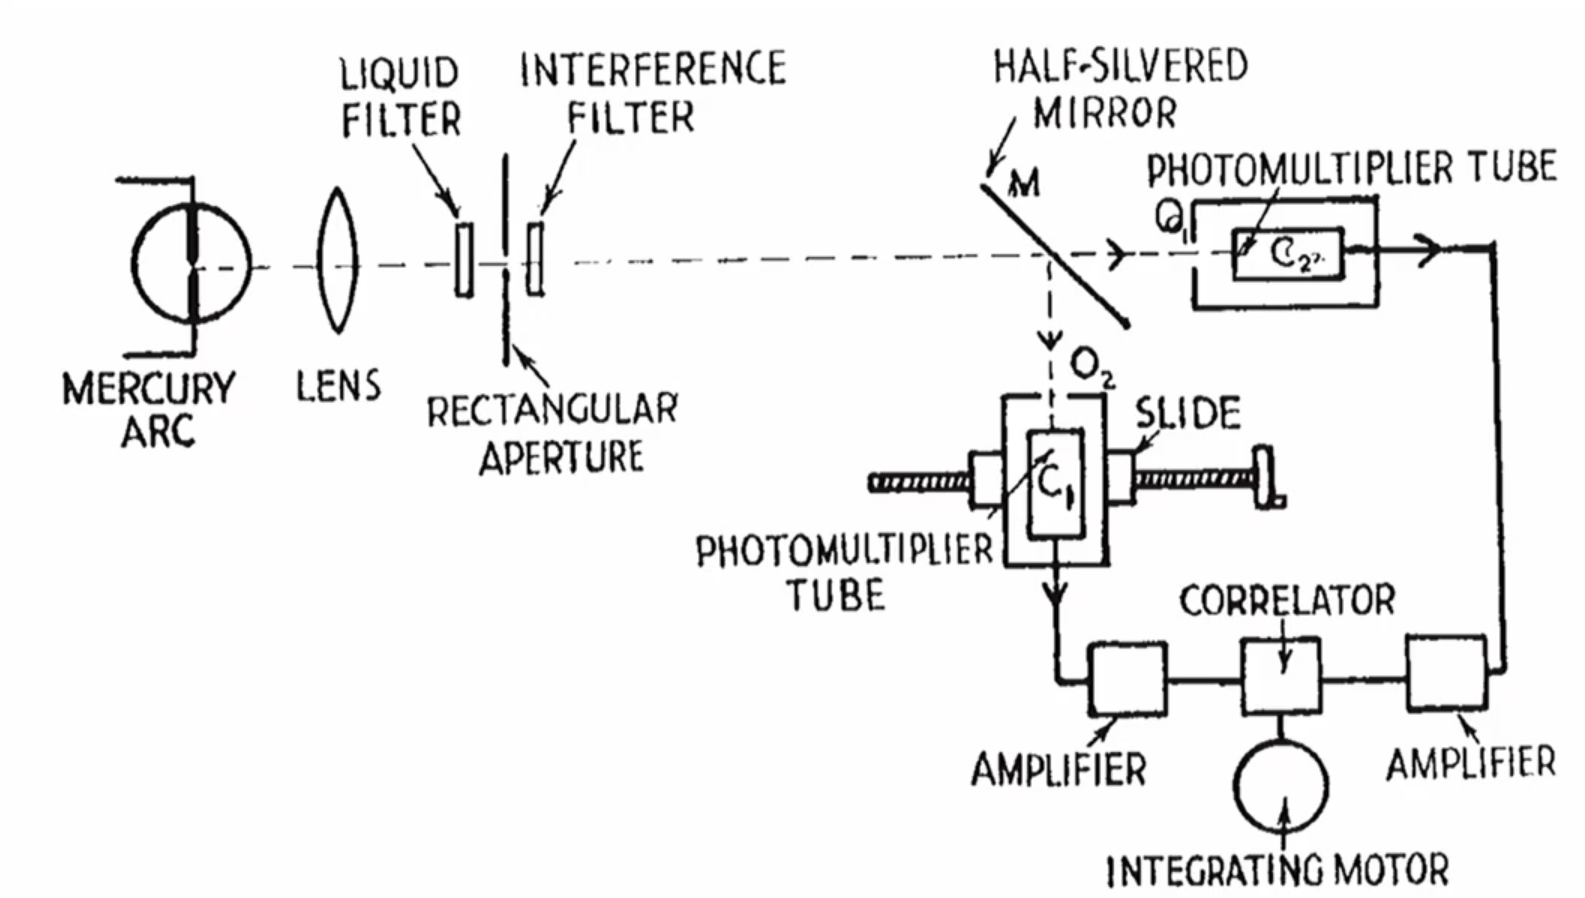
\includegraphics[width=0.6\linewidth]{images_in_png/Grafico_52a.png}
\end{figure}
\begin{itemize}
    \item As a source, Hanbury Brown and Twiss used a mercury lamp emitting at $\lambda = \qty{435.8}{\nano\meter}$;
    \item The signal passes through lenses and filters, so that it becomes collimated and spectrally selected;
    \item It then reaches a $50:50$ beam splitter, and each output is sent to a photomultiplier tube;
    \item The two output signals are amplified and fed into a correlator, which measures the average product of the intensity fluctuations over long observation times.
\end{itemize}
We assume that the detectors are placed symmetrically, so that the two optical paths are identical. Then
\[
I_1(t)=I_2(t)\equiv I(t),
\]
with
\[
I(t)=\langle I(t)\rangle+\Delta I(t).
\]
Here $2I(t)$ is the total intensity incident on the beam splitter, while $\Delta I(t)$ represents the fluctuations around the mean value. The output of the correlator is proportional to
\[
\langle \Delta I(t)\,\Delta I(t+\tau)\rangle.
\]
At $\tau=0$, the two paths are identical and
\[
\langle \Delta I^2(t)\rangle\neq 0,
\]
while
\[
\langle \Delta I(t)\rangle=0.
\]
When $|\tau|\gg\tau_c$, the fluctuations become uncorrelated, so
\[
\langle \Delta I(t)\,\Delta I(t+\tau)\rangle \to 0.
\]
Therefore, measuring the output as a function of $\tau$ provides information about the coherence time $\tau_c$. In the original HBT interferometer, varying the detector separation was used to probe the spatial coherence of the source rather than its temporal coherence.

\subsection{Bunched and anti-bunched light in HBT}
Here a simplified scheme of the HBT interferometer is presented:
\begin{figure}[H]
    \centering
    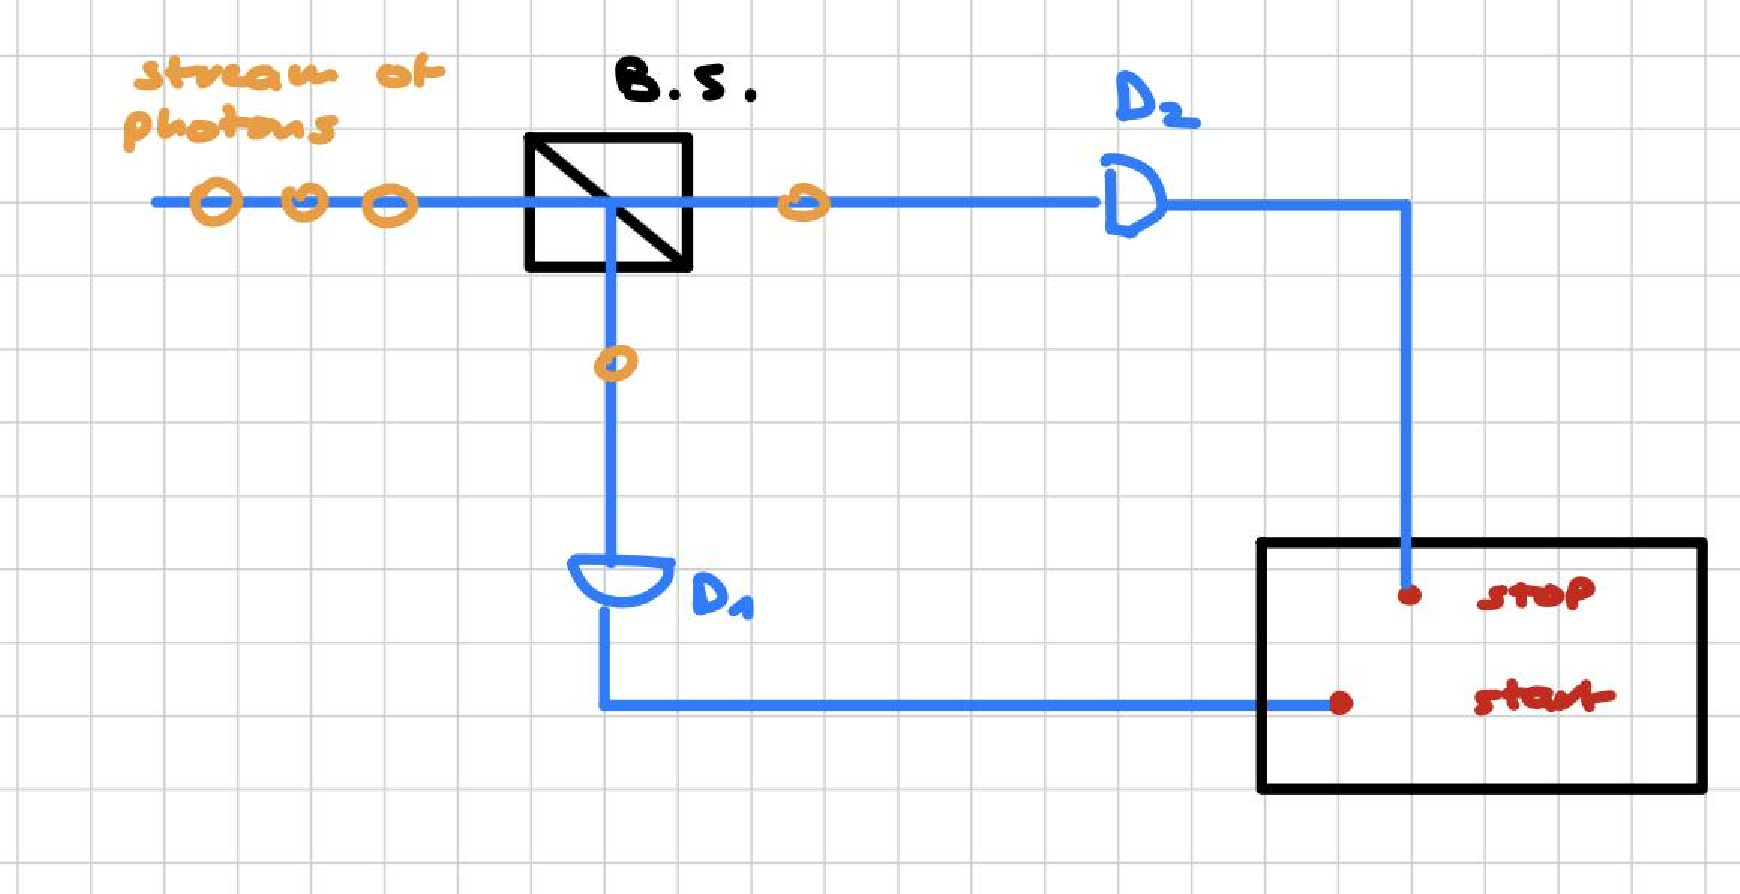
\includegraphics[width=0.6\linewidth]{images_in_pdf/10-/Grafico_53.pdf}
\end{figure}

The light beam is sent to a beam splitter. The reflected part reaches detector $D_1$ and starts the timing electronics, while the transmitted part reaches detector $D_2$ and provides the stop signal. In this way, we count the number of coincidence events while measuring the time delay between the two detectors.\\
The second-order correlation function $g^{(2)}(\tau)$ is proportional to the conditional probability of detecting a second photon at $D_2$ at time $t=\tau$, given that another photon has been detected at $D_1$ at time $t=0$.\\
The Hanbury Brown and Twiss interferometer provides a direct measurement of $g^{(2)}(\tau)$. If we define $n_i(t)$ as the number of counts registered by detector $D_i$ at time $t$, then:
\begin{equation}\label{eqn:10-second-order-correlation-function-photon-counting}
g^{(2)}(\tau)=\frac{\langle n_1(t)\,n_2(t+\tau)\rangle}{\langle n_1(t)\rangle\,\langle n_2(t+\tau)\rangle}.
\end{equation}

\hl{Since $n_i \propto I$}, we can build a histogram that shows the number of coincidence events observed within a given time interval:
\begin{figure}[H]
    \centering
    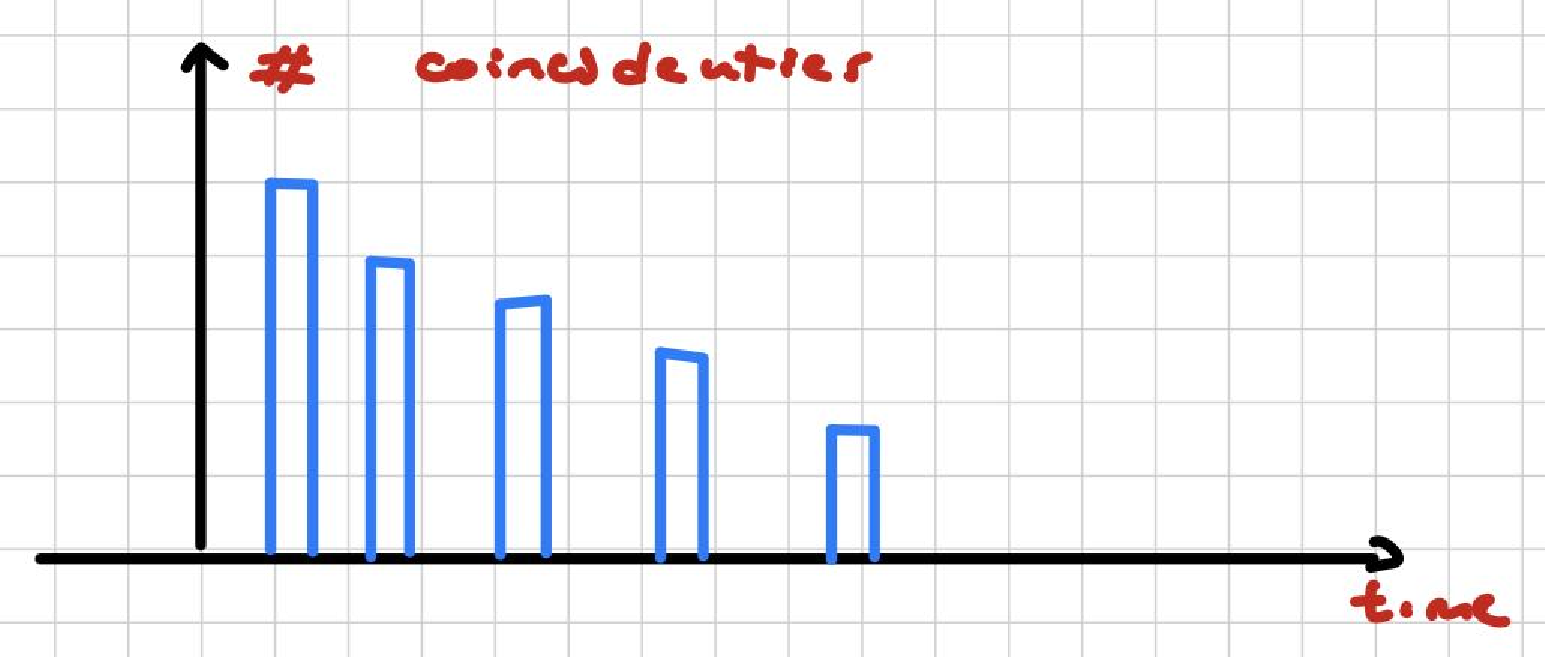
\includegraphics[width=0.6\linewidth]{images_in_pdf/10-/Grafico_54.pdf}
\end{figure}

\calloutinfo{%
\begin{itemize}
    \item \textbf{If we are dealing with a stream of well-separated photons}, there is a $50\%$ probability that one photon is reflected to $D_1$ and starts the timer, but the same photon cannot also generate a stop signal at $D_2$. Therefore, ideally, we expect no coincidences at $\tau=0$. The next photon may later be transmitted to $D_2$ and stop the timer, so coincidence events appear only at nonzero delays. This means that the conditional probability of detecting a second photon immediately after the first one is suppressed, and thus
    \begin{equation}\label{eqn:10-photon-antibunching}
    g^{(2)}(0) < g^{(2)}(\tau),
    \end{equation}

    which is a signature of nonclassical light. This is the case of \textbf{anti-bunched light}, namely a stream of individual photons separated in time by emission dynamics rather than by classical randomness.

    \item\textbf{On the other hand, if many photons arrive in groups}, then both detectors have a high probability of clicking at nearly the same time. In that case, the coincidence histogram shows a large peak around $\tau=0$, and the correlation function decreases as $\tau$ increases because the probability of detecting two photons from the same bunch becomes smaller. This is the typical behavior of \textbf{bunched light}, which is characteristic of chaotic classical sources.
\end{itemize}
}

\subsection{Light classification in terms of $g^{(2)}(0)$}

At the end, we obtain a way to classify light according to the value of $g^{(2)}(0)$:
\begin{enumerate}
    \item \textbf{Coherent light:} Poissonian statistics with random time intervals between photons, where
    \[
    g^{(2)}(\tau)=1 \qquad \forall\,\tau.
    \]

    The probability of obtaining a stop pulse is the same at any delay, and in particular
    \[
    g^{(2)}(0)=1.
    \]

    \item \textbf{Bunched light:}
    \begin{figure}[H]
        \centering
        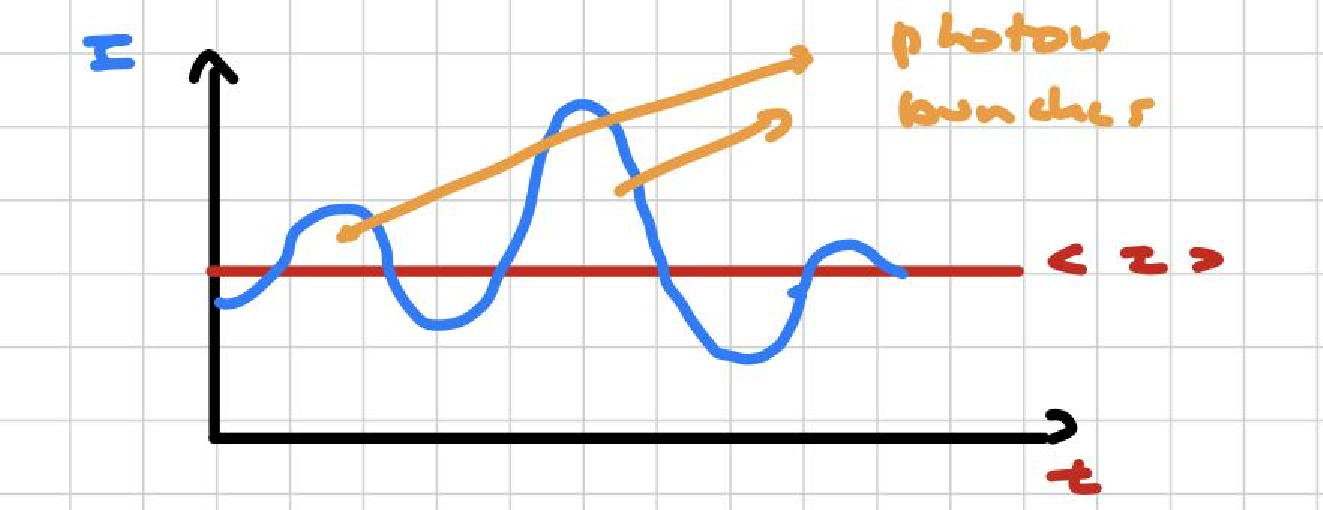
\includegraphics[width=0.6\linewidth]{images_in_pdf/10-/Grafico_55.pdf}
    \end{figure}
    \[
    g^{(2)}(\tau)=
    \begin{cases}
        \text{large for small } \tau,\\
        \text{small for large } \tau,
    \end{cases}
    \qquad \Rightarrow \qquad g^{(2)}(0)>g^{(2)}(\infty).
    \]

    This is the typical behavior of classical chaotic light sources.

    \item \textbf{Anti-bunched light:} the photons are emitted with regular gaps, and there is no classical counterpart for this behavior:
    \begin{figure}[H]
        \centering
        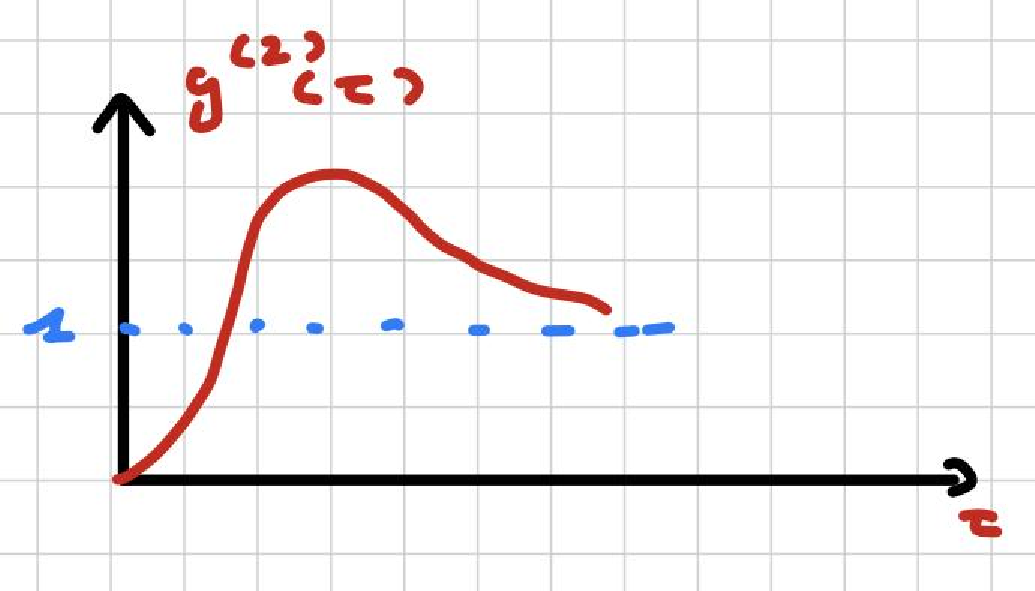
\includegraphics[width=0.6\linewidth]{images_in_pdf/10-/Grafico_56.pdf}
    \end{figure}
    \[
    g^{(2)}(0)<g^{(2)}(\tau), \qquad g^{(2)}(0)<1.
    \]
\end{enumerate}

\calloutwarn{Note that sub-poissonian light is also a clear signature of the quantum nature of light. However, photon antibunching and sub-poissonian statistics \textbf{are distinct nonclassical effects}: they may occur together, but one can also appear without the other.}

\subsection{Experimental demonstration of photon antibunching}
The first experimental demonstration of photon antibunching was provided by Kimble and coworkers:
\begin{itemize}
    \item They sent a dilute beam of sodium atoms along a collimated stream, so that only a very small number of atoms contributed to the fluorescence at any given time;
    \item The atoms were excited by a light beam, and each atom could emit a photon;
    \item The emitted photons were collected by a microscope system;
    \item The light passed through additional optics and a beam splitter, and each output reached a photomultiplier tube;
    \item Each output was amplified and sent through a discriminator;
    \item Finally, the signals were sent to coincidence electronics, one channel providing the start and the other the stop.
\end{itemize}

\calloutwarn{%
    Notice that in a discharge lamp the light is emitted by millions of atoms, each one statistically independent, and this leads to bunched thermal light. In this experiment, instead, \emph{at any given time only one or a few atoms effectively contribute to the fluorescence}, which makes antibunching observable. 
}
\begin{figure}[H]
    \centering
    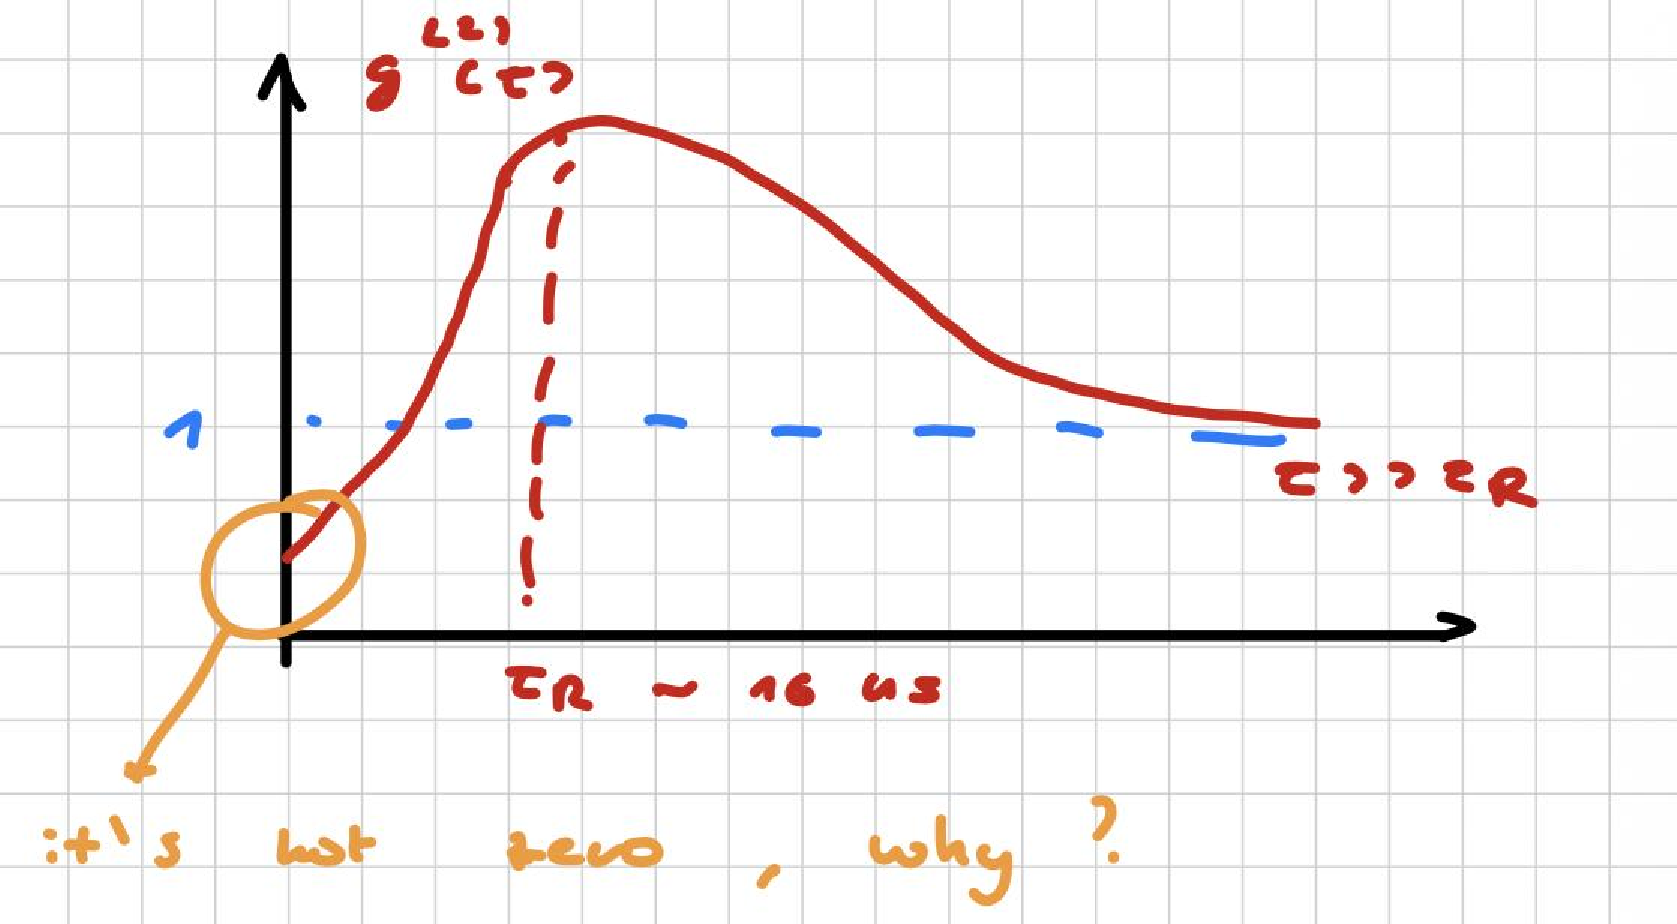
\includegraphics[width=0.6\linewidth]{images_in_pdf/10-/Grafico_57.pdf}
\end{figure}

The observed behavior is:
\begin{itemize}
    \item Ideally, one expects $g^{(2)}(0)=0$. Experimentally, the value is not exactly zero because of detector dark counts, background light, finite time resolution, and the possibility of accidental coincidences.
    \item Then $g^{(2)}(\tau)$ rises on a time scale comparable to the radiative lifetime of the atomic ensemble, $\tau_R \approx 16\,\mathrm{ns}$.
    \item For $\tau \gg \tau_R$, the correlation function decreases toward unity:
    \[
    g^{(2)}(\tau)\to 1.
    \]
\end{itemize}

\hl{This was the first experimental evidence of single-photon emission from a single atom and of anti-bunched light}.

Here a table to sum up the different types of light is provided:

\begin{table}[H]
\centering
\begin{tabular}{@{}ccc@{}}
\toprule
\textbf{Type}         & \textbf{Second order correlation function}                    & \textbf{Source}    \\ \midrule
\textit{Coherent}     & $g^{(2)}(\tau) = 1, \hspace{1ex}\forall \, \tau$ & Classical coherent \\[0.75ex]
\textit{Bunched}      & $g^{(2)}(\tau) < g^{(2)}(0)$                                  & Classical          \\[0.75ex]
\textit{Anti-bunched} & $g^{(2)}(\tau) > g^{(2)}(0)$                                  & Not-classical      \\ \bottomrule
\end{tabular}
\end{table}

\subsection{Single-photon sources}
Single-photon sources must satisfy two fundamental requirements:
\begin{itemize}
    \item the ability to isolate individual emitting species;
    \item the possibility to control the rate at which photons are emitted.
\end{itemize}
To realize such a source, one considers the emission of a single photon in response to an optical or electrical trigger. Let us select an emitting species and examine its energy-level structure.
\begin{figure}[H]
    \centering
    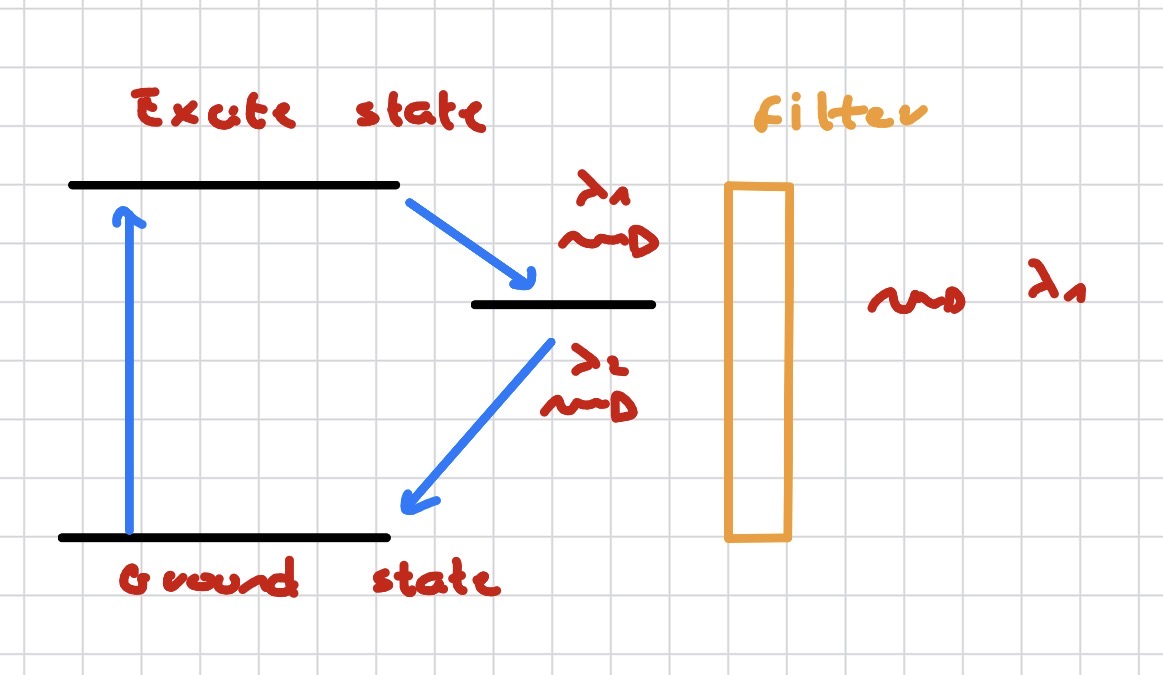
\includegraphics[width=0.6\linewidth]{images_in_png/Grafico_58.jpg}
\end{figure}
The ground state is first excited to a higher-energy state. During relaxation, the system may pass through intermediate states, which can emit photons with different wavelengths $\lambda_1,\lambda_2,\dots$. By inserting suitable optical filters, one can select a specific wavelength and reject the others. In this way, \hl{an optical or electrical pulse acts as a trigger that promotes the electron to an excited state, and the emitter releases one photon after a characteristic radiative lifetime $\tau_R$} for each excitation cycle. The time between two trigger pulses is
\[
T=\frac{1}{f_T},
\]
where $f_T$ is the trigger repetition rate.
\begin{figure}[H]
    \centering
    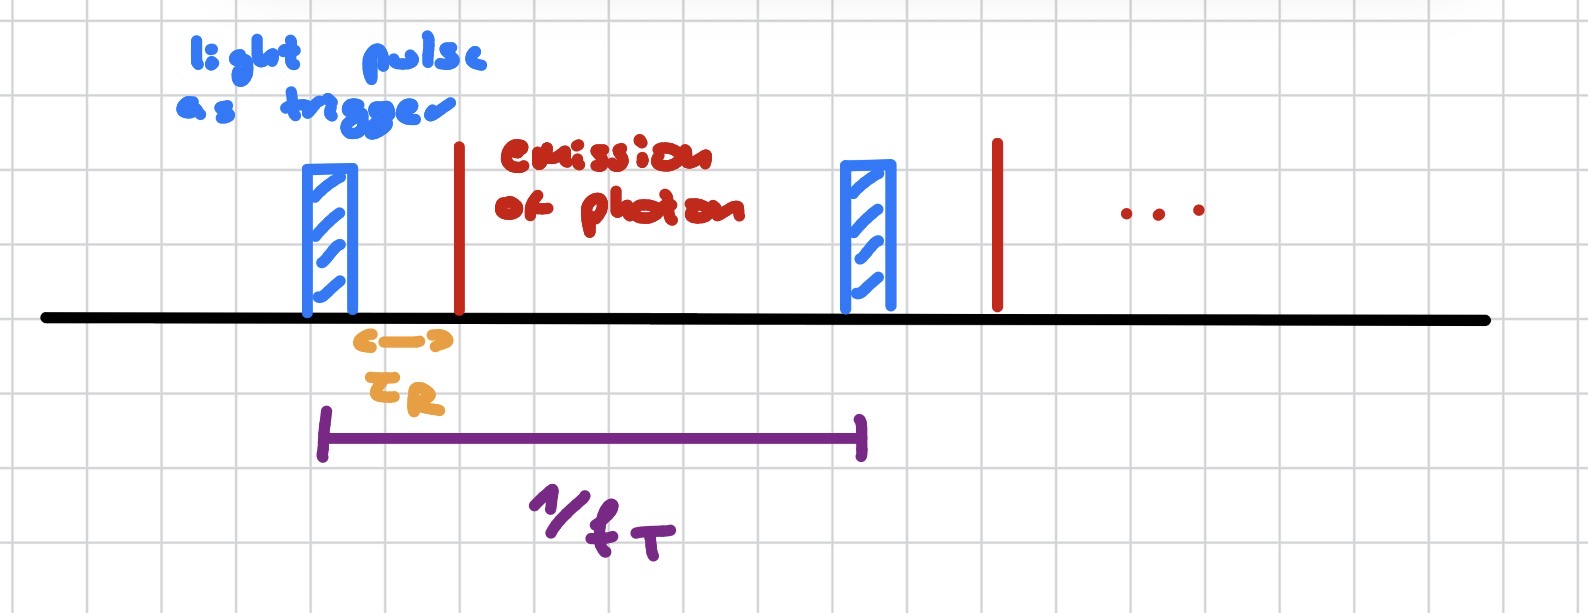
\includegraphics[width=0.6\linewidth]{images_in_png/Grafico_59.jpg}
\end{figure}
No new photon can be emitted until the next trigger pulse arrives.

If
\[
\frac{1}{f_T} = T >\tau_R,
\]
the trigger controls the temporal separation between successive emission events, and the source can exhibit anti-bunched light.

The fluorescence process remains probabilistic, so the photon stream is not perfectly regular. However, the \hl{probability of emitting two photons within a time interval much shorter than $\tau_R$ is very small}, which implies
\[
g^{(2)}(0)\approx 0.
\]

\calloutinfo{%
The use of solid-state emitters instead of atoms is extremely attractive because they are fixed in the lattice and can therefore be integrated into practical devices. Moreover, quantum confinement leads to discrete energy levels, so these nanostructures behave as \textit{artificial atoms}. In a simple confinement picture, the energy levels scale approximately as
\[
E_n \propto \frac{n^2}{L^2},
\]
so that by changing the size of the nanostructure one can select different emission wavelengths for different physical applications.
}

\subsection{Spectroscopy of single semiconductor nanocrystals}
By means of \textbf{molecular beam epitaxy (MBE)} one can fabricate ensembles of nanostructures that are not perfectly identical. They differ in shape, size, defects, surface states, chemical composition, and impurity content. All these factors affect the energy levels $E_n$ and the emission properties. \hl{What is measured experimentally in an ensemble is therefore an average over many different objects}, which produces a large \textbf{inhomogeneous broadening}.

\question{Can we measure the spectra of individual low-dimensional objects?}{
Yes. The first experiments of this kind were performed using optical spectroscopy with high spatial resolution.}

\subsubsection{Potential limitations}

Quantum confinement becomes relevant when the characteristic size of the nanostructure is comparable to the exciton\footnote{An exciton is a bound state of an electron and a hole interacting through the Coulomb potential.} Bohr radius, which is typically of the order of $\sim 10\,\mathrm{nm}$.

However, spatial resolution is limited by diffraction. According to the \textbf{Rayleigh criterion}, two point sources are distinguishable if their separation is at least of the order of the distance between the center of the Airy disk and its first minimum:
\[
d \gtrsim 0.61\,\frac{\lambda}{\mathrm{NA}},
\]
where $\mathrm{NA}$ is the numerical aperture of the objective. 
\calloutwarn{%
    For a common microscope objective, this gives a resolution limit of the order of $10^2\,\mathrm{nm}$, which is much larger than the typical size of a quantum dot.
}
\textbf{But} we are not trying to image the true size of the object itself; instead, \hl{we just want to detect the luminescence signal emitted by a single quantum dot and distinguish it from all other signals}. The following conditions are therefore required:
\begin{enumerate}
    \item the density of objects must be low, so that the \hl{distance between them is larger than the diffraction-limited resolution};
    \item parasitic light sources must be suppressed;
    \item the spatial resolution and image quality must be as high as possible;
    \item the emitted photons must be collected efficiently, which requires a high quantum efficiency $\eta$.
\end{enumerate}
If we take a spot of \qty{200}{\micro\meter}, we expect roughly $10^7$ quantum dots and therefore a broad emission spectrum. If instead we achieve a spot of \qty{200}{\nano\meter}, we can isolate a few emitters and observe sharp lines, leading to spatially resolved photoluminescence from a single quantum dot. 

To achieve this, we need:
\begin{itemize}
    \item a microscope for spatial resolution operating near the diffraction limit;
    \item a spectroscopic system for spectral resolution. The sample is excited by a laser beam inside a cryogenic device, and the emitted photons are collected in an \textbf{epifluorescence} geometry, meaning that excitation and collection occur along the same optical path. A \textbf{grating} provides spectral dispersion, while filters are used to select specific wavelengths.
\end{itemize}
\textbf{Scanning technique (confocal effect):}

To augment our resolution, we can use two lenses and an optical axis. Suppose a source is placed on the optical axis and its light is collected by both lenses and sent to a spectrometer. If a pinhole is inserted between the lenses, the spatial resolution improves because light coming from sources away from the optical axis is blocked by the iris (i.e., the pinhole along with the optical axis). In this way, out-of-focus contributions are strongly suppressed.
\begin{figure}[H]
    \centering
    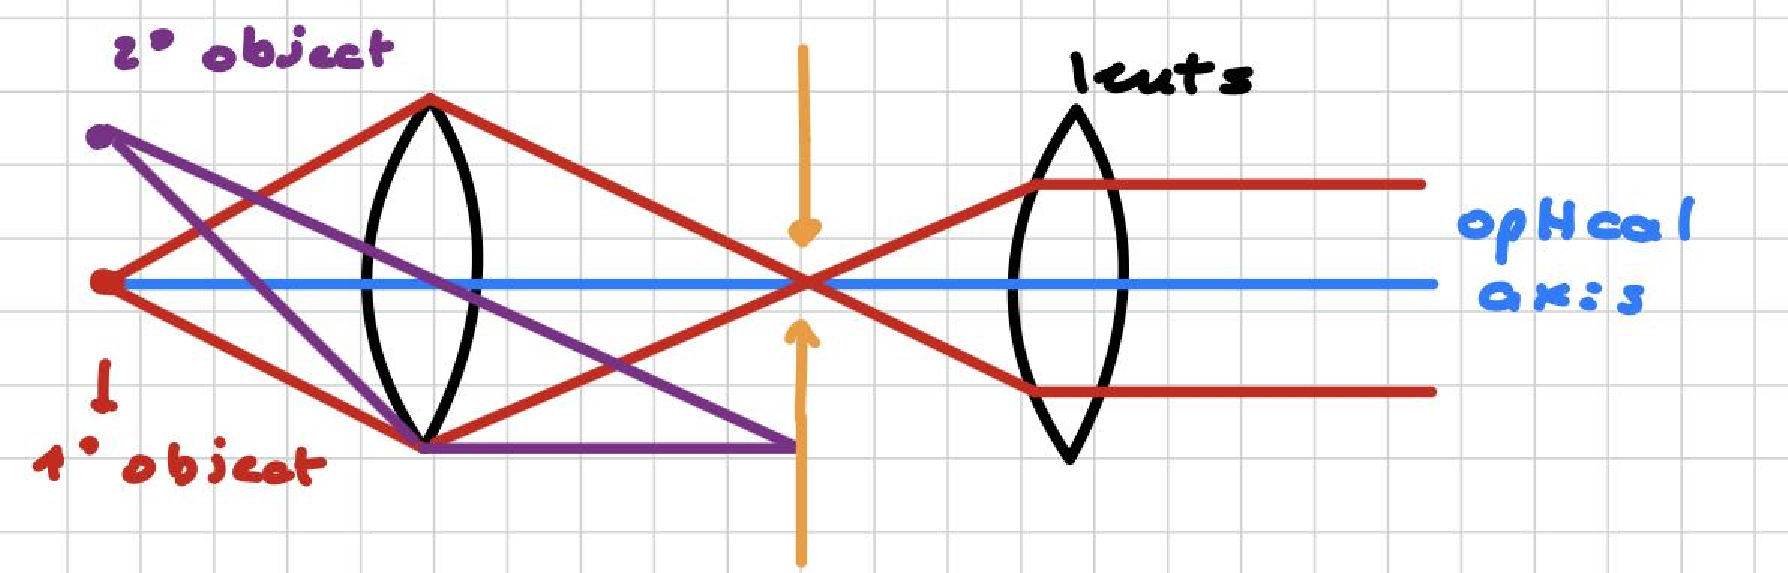
\includegraphics[width=0.6\linewidth]{images_in_pdf/10-/Grafico_60.pdf}
\end{figure}

Scanning is achieved either by moving the sample, which is glued on an $x,y,z$ stage, or by moving the excitation spot using piezo-positioned mirrors. The sample is illuminated by a laser beam, and for each position the emission spectrum is measured. In this way, one reconstructs a three-dimensional map of the material emission. The emitted light is collected along the same path (epifluorescence), passes through a dichroic mirror\footnote{A dichroic mirror is a mirror that reflects certain wavelengths while transmitting others.} and the optical system described above, and is then directed toward a beam splitter.
The two outputs (the reflected beam and the fluorescence one) go directly in two detectors and can be used either to measure the fluorescence lifetime with time-correlated single-photon counting or to study light statistics through the second-order correlation function.
\begin{figure}[H]
    \centering
    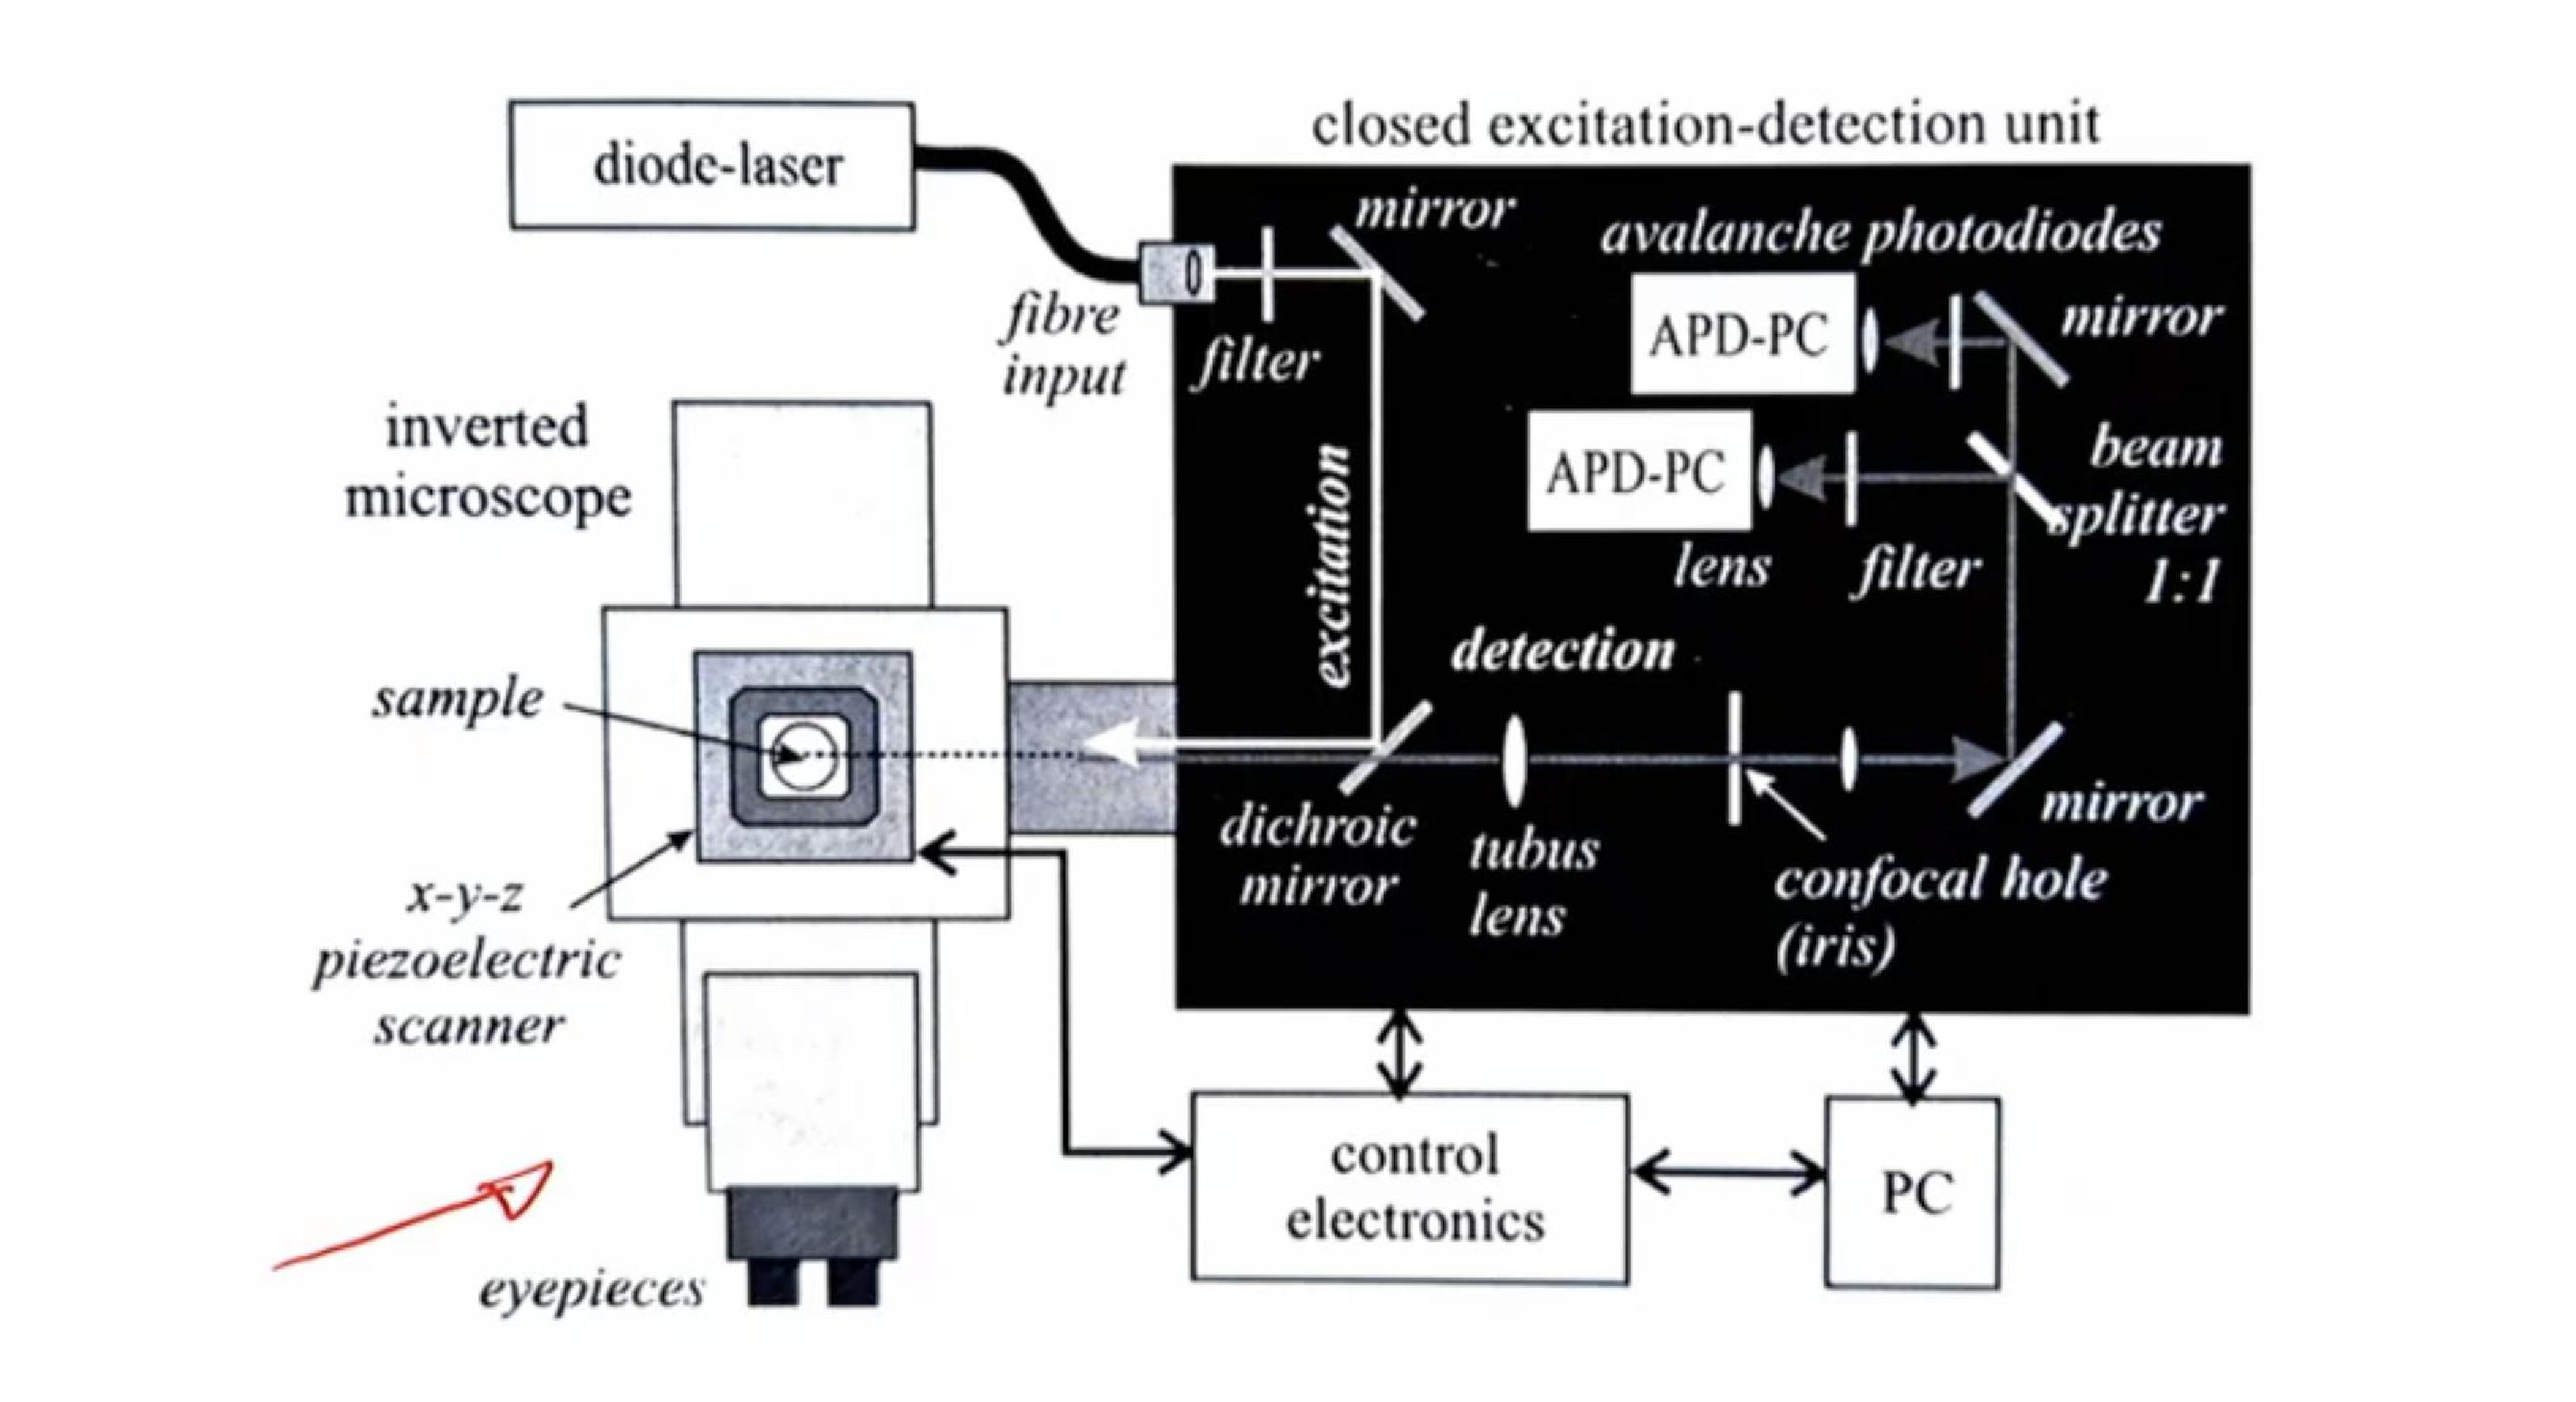
\includegraphics[width=0.6\linewidth]{images_in_pdf/10-/Grafico_61.pdf}
\end{figure}

Compared with an ensemble, the photoluminescence of individual nanocrystals always shows much narrower spectral lines, whose width is ultimately limited by the radiative lifetime $\tau_R$, by means of the energy-time uncertainty principle (Eqn.~\ref{eqn:6-energy-time-uncertainty}). In the lifetime-limited case, the linewidth scales as
\[
\Delta E \sim \frac{\hbar}{\tau_R},
\]

so for $\tau_R \approx \qty{1}{\nano\second}$ the spectral width is typically of the order of $\unit{\micro\electronvolt}$.

\subsubsection{Example: QD with InAs}
\begin{figure}[H]
    \centering
    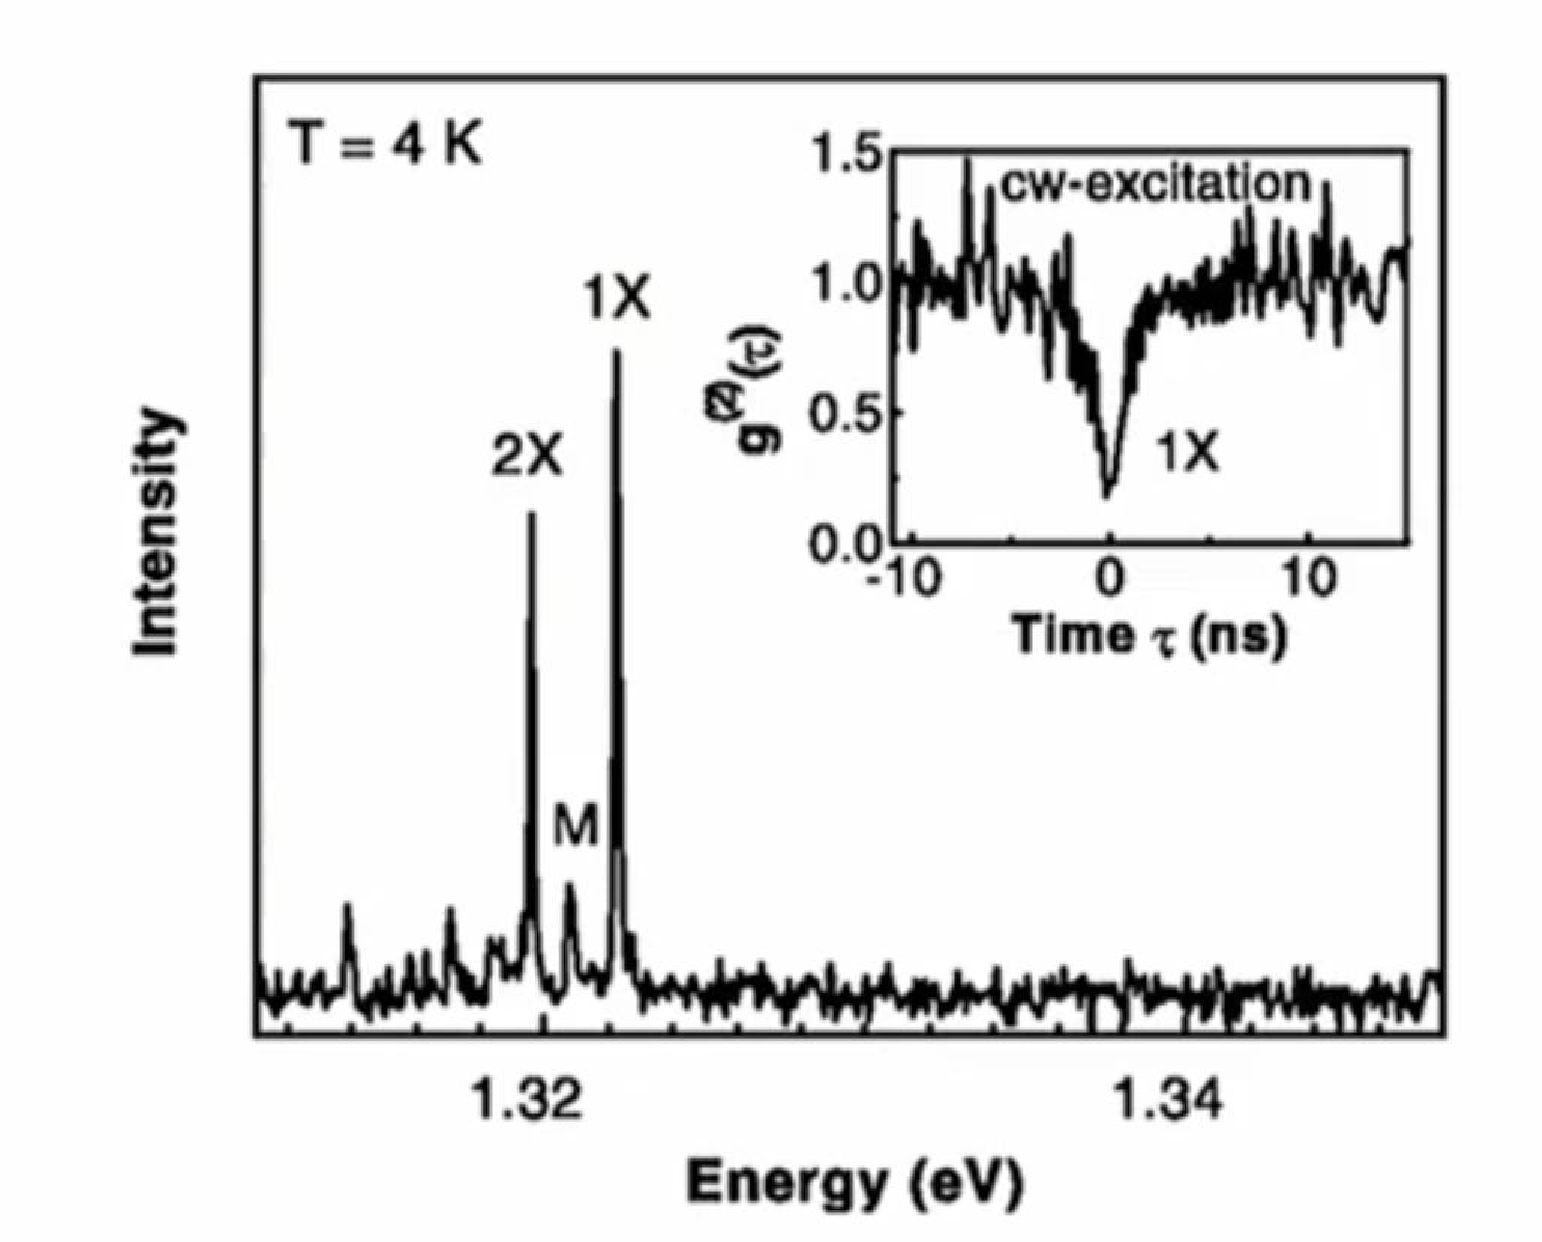
\includegraphics[width=0.6\linewidth]{images_in_pdf/10-/Grafico_62.pdf}
\end{figure}

The peak labeled $1X$ corresponds to exciton recombination, while $2X$ corresponds to bi-exciton recombination. The second-order correlation function is close to zero, with a typical experimental value of about $g^{(2)}(0)\approx 0.2$, which is a clear signature of an anti-bunched light source. 

\question{But why is it not exactly zero?}{%
The answer is that the detector time response, about \qty{0.4}{\nano\second}, must be compared with the radiative lifetime of about \qty{2.2}{\nano\second}. There is therefore a nonzero probability of detecting two events within a time interval that the detector cannot fully resolve (i.e. both events are considered at $t=0$). This is why the time jitter of the detector is so important.
}

We can illustrate this with a numerical example:
\begin{figure}[H]
    \centering
    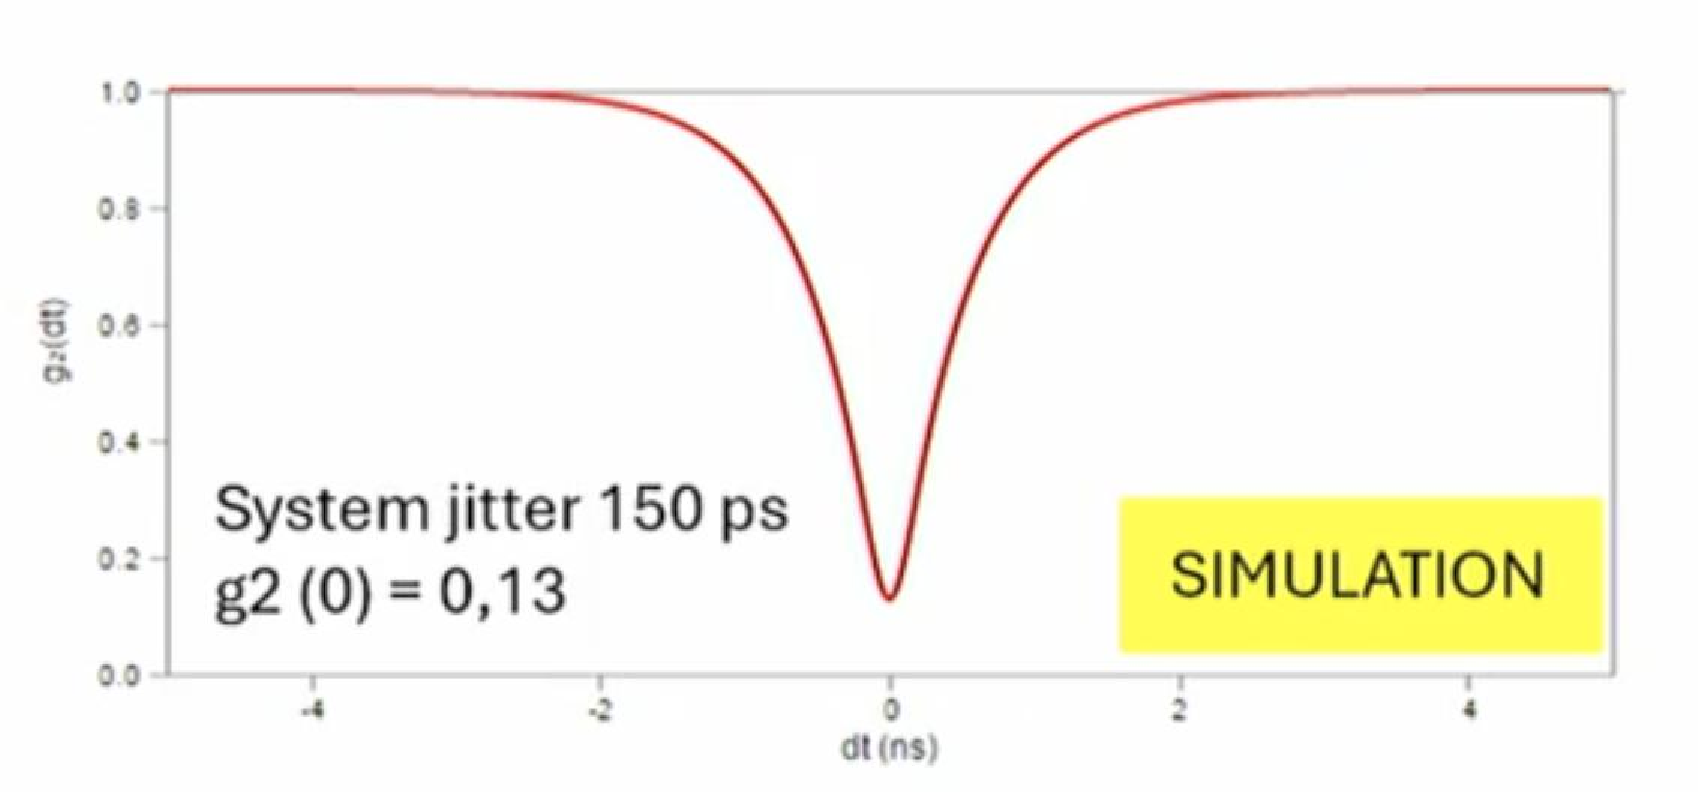
\includegraphics[width=0.6\linewidth]{images_in_pdf/10-/Grafico_63.pdf}
\end{figure}

\begin{figure}[H]
    \centering
    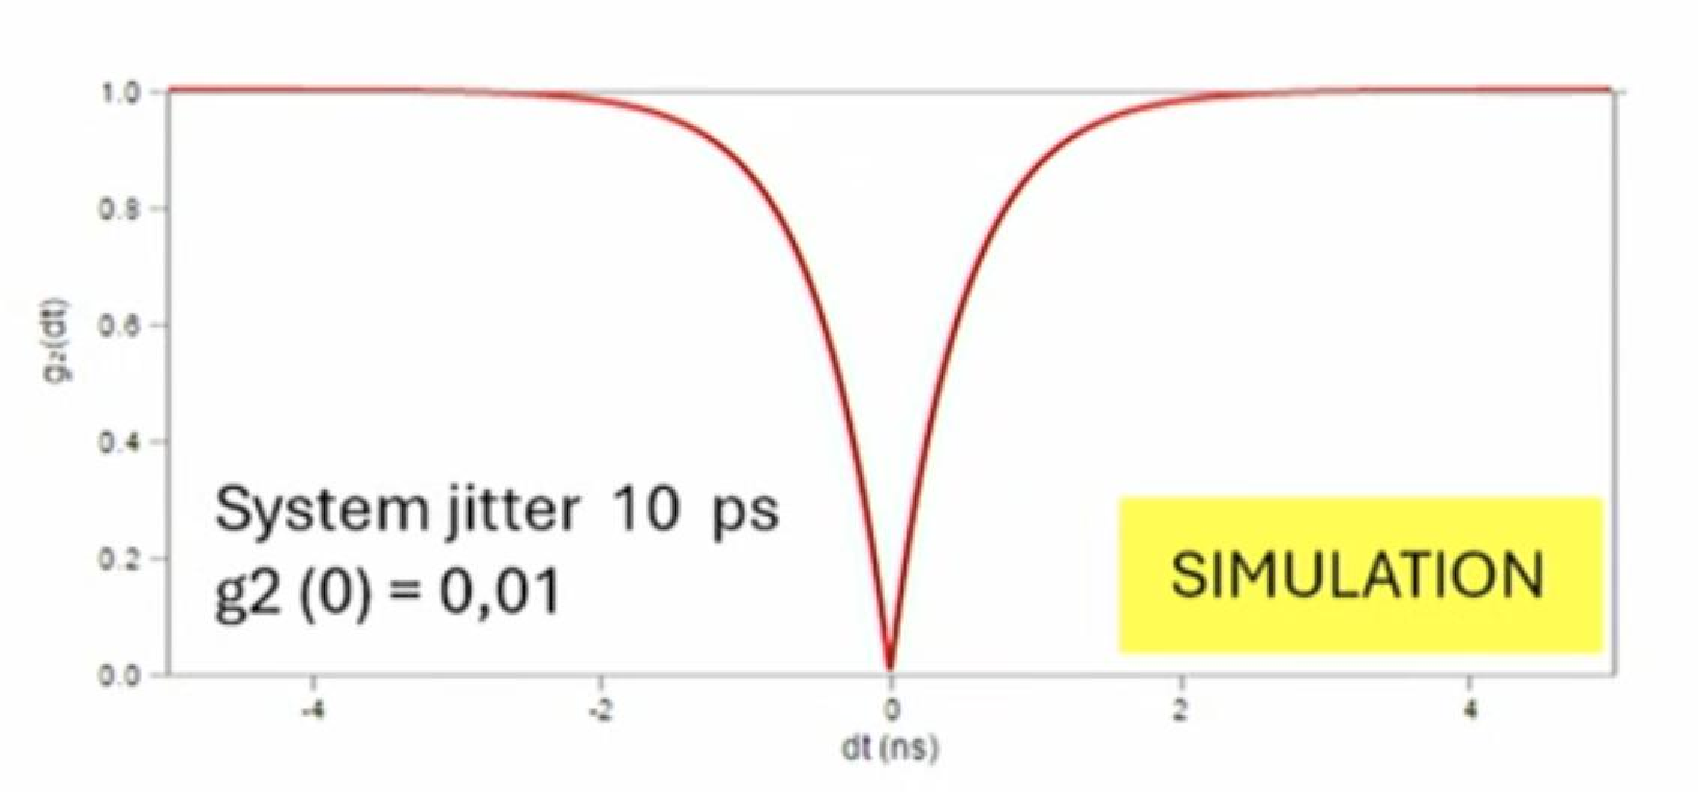
\includegraphics[width=0.6\linewidth]{images_in_pdf/10-/Grafico_64.pdf}
\end{figure}

If the time jitter of the detector is reduced, the measured value of $g^{(2)}(0)$ approaches zero.


\chapter{Purely quantum light}\label{chap:11-purely-quantum-light}

\section{Electro-magnetic field quantization}\label{sec:11-em-field-quantization}

\subsection{Physical context}\label{subsec:11-physical-context}

\subsubsection{EM cavity}

\begin{figure}[H]
    \centering
    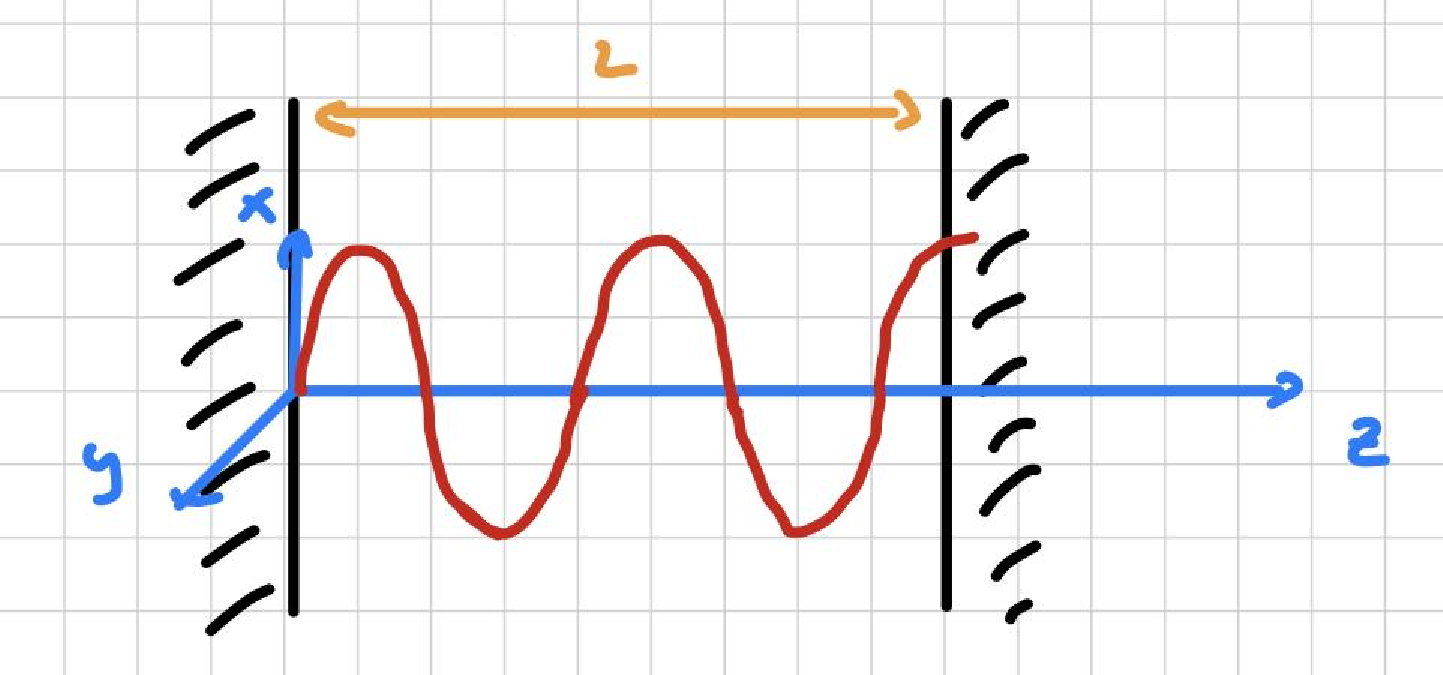
\includegraphics[width=0.6\linewidth]{images_in_pdf/11-/Grafico_65.pdf}
\end{figure}

Suppose that:
\begin{itemize}
    \item the radiation field is confined in a one-dimensional cavity along the $z$-axis, with perfectly conducting walls at $z=0$ and $z=L$ (i.e. no field can escape from the cavity);
    \item the boundary condition $\vec{E}=0$ at the walls implies standing waves;
    \item the electric field is polarized along $\hat{x}$;
    \item there are no charges, no currents, and no dielectric material in the cavity, so the field propagates in vacuum.
\end{itemize}

The Maxwell equations in differential form reduce to
\begin{equation}\label{eqn:11-maxwell-eqs}
\begin{cases}
\vec{\nabla}\times\vec{E}=-\pdv{\vec{B}}{t}\\[1ex]
\vec{\nabla}\,\vec{E}=0\\[1ex]
\vec{\nabla}\times\vec{B}=\mu_0\epsilon_0\pdv{\vec{E}}{t}\\[1ex]
\vec{\nabla}\,\vec{B}=0
\end{cases}
\end{equation}

and the electric field of a single mode $m$ can be written as
\begin{equation}\label{eqn:11-single-mode-electric-field}
\begin{aligned}
&\vec{E}_{m}(z,t) = E_{m}(z,t)\,\hat{x} =
\,E_0\sin(k_m z)\sin(\omega_m t)\,\hat{x},\\[1ex]
\text{where:}\hspace{2ex}
&k_m = \frac{m\pi}{L},
\hspace{2ex}
\omega_m=ck_m=\frac{m\pi c}{L},
\hspace{2ex}
m=1,2,3,\dots
\end{aligned}
\end{equation}

in which the allowed frequencies are fixed by the boundary conditions of the cavity.

Since the magnetic field must be orthogonal both to the electric field and to the propagation direction, it follows that:
\begin{gather}
\vec{B}(\vec{r},t) = B_y(z,t)\,\hat{y}\\[1ex]
\vec{\nabla} \times \vec{B} = 
\mu_0 \epsilon_0\, \pdv{\vec{E}}{t} 
\implies - \pdv{B_y}{t} = 
\mu_0 \epsilon_0\, \pdv{E_x}{t} \\[1ex]
\implies B_y(z,t) = B_0 \cos(kz) \cos(\omega t)
\end{gather} 

with $B_0=E_0/c$, so that the two fields satisfy Maxwell equations and are phase-shifted by $\pi/2$.

\subsubsection{Energy and harmonic oscillator analogy}

If we define $V=LA$ as the effective cavity volume, the classical energy of a single mode is
\begin{equation}\label{eqn:11-single-mode-classical-energy}
H_m = \frac12\int_V dV
\left[
    \epsilon_0 E^2_{m}(\vec r,t)+\frac{1}{\mu_0}B^2_{m}(\vec r,t)
\right] =
\frac12\int_V dV
\left[
    \epsilon_0 E_{m,x}^2(z,t)+\frac{1}{\mu_0}B_{m,y}^2(z,t)
\right].
\end{equation}

Separating the electric and magnetic contributions, we obtain
\begin{equation}\label{eqn:11-single-mode-electric-energy}
\begin{split}
    U_{el.} &= \frac{1}{2}\epsilon_0 A\, \int_0^L dz \, E_0^2\, sin^2(kz)\, \sin^2(\omega t) = \\[1ex]
    &= \frac{1}{4}\epsilon_0 A\, E_0^2\, \sin^2(\omega t) \, \int_0^L dz \, [1-\cos(2kz)] = \\[1ex]
    &=\frac{1}{4}\epsilon_0 A\, E_0^2\, \sin^2(\omega t) \, \bigl(L-\frac{\sin(2kL)}{2k}\bigr)
\end{split}
\end{equation}

The term $\sin(2kL)= 0$  for the boundary conditions, so we obtain:
\begin{equation}\label{eqn:11-single-mode-electric-energy-2}
U_{el.}=\frac{1}{4}\epsilon_0\, V\, E_0^2\, \sin^2(\omega t)
\end{equation}

For the magnetic term we have:
\begin{equation}\label{eqn:11-single-mode-magnetic-energy}
\begin{split}
    U_{M} &= \frac{1}{2\mu_0} A\, \int_0^L dz \, B_0^2\, \cos^2(kz)\, \cos^2(\omega t)= \\[1ex]
    &= \frac{1}{4\mu_0} A\, B_0^2\, \cos^2(\omega t) \, \int_0^L dz \, [1+\cos(2kz)]= \\[1ex]
    &=\frac{1}{4\mu_0} A\, B_0^2\, \cos^2(\omega t) \, \bigl(L+\frac{\sin(2kL)}{2k}\bigr) = \\[1ex]
    &= \frac{1}{4\mu_0}\, V\, B_0^2\, \cos^2(\omega t)
\end{split}
\end{equation}

Therefore,
  \[H = U_{el.}+U_M = \frac{V}{4}\biggr[\epsilon_0 \, E_0^2\, \sin^2(\omega t)+\frac{1}{\mu_0}\, B_0^2\, \cos^2(\omega t)\biggr]\]

\calloutinfo{%
Energy is continuously exchanged between the electric and magnetic parts. This is formally analogous to the exchange between kinetic and potential energy in a harmonic oscillator:
\begin{equation}\label{eqn:11-harmonic-oscillator-energy}
H=\frac{p^2}{2m}+\frac12 m\omega^2 x^2.
\end{equation}
}

\subsection{Quantization in the harmonic oscillator picture}\label{subsec:11-quantization-harmonic-oscillator}

\subsubsection{Hamiltonian and Schrödinger equation}

Promoting $H$ to its quantum version $\hat{H}$, we can write the time-independent Schrödinger equation for the field mode:
\begin{equation}\label{eqn:11-time-independent-schrodinger-equation}
\hat H\psi=E\psi,
\hspace{2ex}
\hat H=\frac{1}{2m}\left[\hat p_x^2+m^2\omega^2\hat X^2\right];
\end{equation}

More explicitly, the equation reads:
\begin{equation}\label{eqn:11-schrodinger-eq-harmonic-potential}
-\frac{\hbar^2}{2m}\frac{d^2\psi}{dx^2}+\frac12 m\omega^2x^2\psi=E\psi.
\end{equation}


If we now introduce the normalized variables
\begin{equation}\label{eqn:11-normalized-variables}
\hat q=\sqrt{m}\,\hat X,
\qquad
\hat p=\frac{1}{\sqrt{m}}\hat p_x,
\end{equation}

then the Hamiltonian becomes
\begin{equation}\label{eqn:11-harmonic-oscillator-hamiltonian-normalized}
\hat H=\frac12\left(\hat p^2+\omega^2\hat q^2\right).
\end{equation}

\calloutinfo{%
This shows that a single electromagnetic mode is formally equivalent to a quantum harmonic oscillator, where the mode amplitudes play the role of canonical coordinate and momentum.
}

If we use the correspondence rule\footnote{The correspondence rule states that the predictions of quantum mechanics must seamlessly reduce to those of classical physics} we can replace classical variables with quantized operators:
\begin{equation}\label{eqn:11-quantized-field-operators}
    \begin{cases}
    \hat{q}(t) = \sqrt{\frac{\epsilon_0V}{2\omega^2}}\, E_0 \, \sin(\omega t)\\[1ex]
    \hat{p}(t) = \sqrt{\frac{V}{2\mu_0}}\, B_0 \, \cos(\omega t) =\sqrt{\frac{\epsilon_0V}{2}}\, E_0 \, \cos(\omega t)
\end{cases}
\end{equation}

Where we use $B_0 = \tfrac{E_0}{c}$ and $c = \tfrac{1}{\sqrt{\epsilon_0\mu_0}}$.
If we extend this argument to all modes we can conclude that by studying the problem of an ideal resonant cavity, we have been led to the conjecture that \hl{the radiation field can be viewed as a collection of quantized simple harmonic oscillator}.

\subsubsection{Annihilation and creation operators}

To construct the Hilbert space of the state vectors related to the radiation field, we need to introduce \emph{annihilation} and \emph{creation} operators $\hat{a}$ and $\hat{a}^\dagger$.
\begin{equation}\label{eqn:11-annihilation-creation-operators-1}
\begin{cases}
    \hat{q} =\sqrt{\frac{\hbar}{2m}}\, (\hat{a}+\hat{a}^\dagger)\\[0.5ex]
    \hat{p} = -i\sqrt{\frac{\hbar \omega }{2}}\, (\hat{a}-\hat{a}^\dagger)
\end{cases}
\end{equation}
inverting:
\begin{equation}\label{eqn:11-annihilation-creation-operators-2}
\begin{cases}
    \hat{a} =\frac{1}{\sqrt{2\hbar \omega}}\, (\omega \hat{q}+i\hat{p})\\[0.5ex]
    \hat{a}^\dagger = \frac{1}{\sqrt{2\hbar \omega}}\, (\omega\hat{q}-i\hat{p})
\end{cases}
\end{equation}
in the means of the original position and momentum operators:
\begin{equation}\label{eqn:11-annihilation-creation-operators-3}
\begin{cases}
    \hat{a} =\frac{1}{\sqrt{2\hbar \omega m}}\, (m\omega \hat{X}+i\hat{p}_x)\\[0.5ex]
    \hat{a}^\dagger = \frac{1}{\sqrt{2\hbar \omega m}}\, (m\omega\hat{X}-i\hat{p}_x)
\end{cases}
\end{equation}

which allows us to rewrite the Hamiltonian as
\begin{equation}\label{eqn:11-hamiltonian-annihilation-creation-operators}
\hat{H} = \hbar \omega \, 
\biggl(\hat{a}^\dagger \hat{a}+\frac{1}{2}\bigr)
\end{equation}

\question{But do these operators commute?}{%
No, they do not. We can verify this by direct calculation:

\begin{proof}
We can verify this by direct calculation:

\begin{align}
\hat{a}^\dagger\hat{a} &= \frac{1}{2m\hbar \omega} \, (m\omega \hat{X}-i\hat{p})\, (m\omega \hat{X}+i\hat{p}) \nonumber \\
&= \frac{1}{2m\hbar \omega} \, [\hat{p}^2+(m\omega \hat{X})^2+im\omega(\hat{X}\hat{p}-\hat{p}\hat{X})] \nonumber \\
&=\frac{1}{\hbar \omega}\, \frac{1}{2m}\,[\hat{p}^2+(m\omega\hat{X})^2]+ \frac{i}{2\hbar}\, [\hat{X},\hat{p}] \nonumber \\
&=\frac{1}{\hbar\omega}\, \hat{H} -\frac{1}{2} \rlap{\hspace{2cm}\text{given } $[\hat{X},\hat{p}]= i\hbar$} \label{eqn:11-commutation-annihilation-creation-operators-proof-1}
\end{align}

Similarly, it can be proven that:
\begin{equation}\label{eqn:11-commutation-annihilation-creation-operators-proof-2}
    \hat{a}\hat{a}^\dagger = 
    \frac{1}{\hbar \omega}\, \hat{H} +\frac{1}{2}
\end{equation}

Therefore:
\begin{equation}\label{eqn:11-commutation-annihilation-creation-operators}
[\hat{a},\hat{a}^\dagger]= \hat{a}\hat{a}^\dagger - \hat{a}^\dagger\hat{a} = 1
\end{equation}
\end{proof}
}

\callout{Proposition: all eigenvalues of $\hat{H}$ are positive}{%
The structure of the Hilbert space is determined by the fact that $\hat{H}$ is a positive operator:
\begin{equation}\label{eqn:11-H-is-positive-operator}
\bra{\psi}\hat{H}\ket{\psi} \geq 0
\end{equation}

For any wawefunction $\psi \in \mathcal{H}$.

\begin{proof}
If we set $\ket{f}=\hat{a}\, \ket{\psi}$ and use $\braket{f|f}\geq 0$:

\begin{equation}\label{eqn:11-H-is-positive-operator-proof}
\begin{split}
    \braket{\psi|\hat{H}|\psi}  &= \hbar \omega \, \braket{\psi|\hat{a}^\dagger\hat{a}|\psi} +\frac{\hbar \omega}{2} = \\
    &=\hbar \omega \braket{f|f} + \frac{\hbar \omega}{2} \geq0\\
\end{split}
\end{equation}
The eigenvalues of $\hat{H}$ are not negative!
\end{proof}
}

\subsubsection{Rising and lowering effects of the annihilation and creation operators}

Given that 
\begin{equation}
    [\hat{H},\hat{a}] = \hat{H}\hat{a}-\hat{a}\hat{H} \implies \hat{H}\hat{a} = [\hat{H},\hat{a}]+\hat{a}\hat{H}
\end{equation}
and if $\ket{u}$ is an eigenstate of $\hat{H}$ with eigenvalue $W$:
\begin{equation}
\hat{H}\hat{a}\, \ket{u} = [\hat{H},\hat{a}]\, \ket{u}+\hat{a}\hat{H}\, \ket{u} = [\hat{H},\hat{a}]\, \ket{u}+\hat{a}W\, \ket{u}
\end{equation}

But: 
\begin{equation}\label{eqn:11-commutator-H-a}
    [\hat{H},\hat{a}] = \hbar \omega [\hat{a}^\dagger\hat{a}, \hat{a}]+
    \bigl[\frac{\hbar \omega }2{,\hat{a}}\bigr]
\end{equation}

The second term is clearly zero, while the first one can be rewritten as:
\begin{equation}
\begin{split}
    [\hat{a}^\dagger\hat{a},\hat{a}] &= \hat{a}^\dagger\hat{a}\hat{a}- \hat{a}\hat{a}^\dagger\hat{a} = \\
    &=\hat{a}^\dagger\hat{a}\hat{a}-\hat{a}^\dagger\hat{a}\hat{a}+\hat{a}^\dagger\hat{a}\hat{a}- \hat{a}\hat{a}^\dagger\hat{a} = \\
    &=\hat{a}^\dagger(\hat{a}\hat{a}-\hat{a}\hat{a})+(\hat{a}^\dagger\hat{a}-\hat{a}\hat{a}^\dagger)\hat{a} = \\
    &=\hat{a}^\dagger[\hat{a},\hat{a}]+[\hat{a}^\dagger,\hat{a}]\hat{a} = \\
    &=\hat{a}^\dagger\, 0 -1\, \hat{a} = \\
    &= - \hat{a}
\end{split}
\end{equation}

so the \eqref{eqn:11-commutator-H-a} becomes:
\begin{equation}
[\hat{H},\hat{a}]= -\hbar \omega \hat{a}
\end{equation}

which means that:
\begin{equation}
\begin{split}
    \hat{H}\hat{a} \, \ket{u} &= 
    -\hbar \omega \hat{a}\, \ket{u}+ \hat{a}\hat{H}\, \ket{u} = \\
    &= -\hbar \omega \hat{a}\, \ket{u}+ E_u\hat{a}\, \ket{u} = \\
    &= (E_u -\hbar \omega) \hat{a}\, \ket{u}\\
\end{split}
\end{equation}

in other words,$\hat{H}\hat{a}\, \ket{u}$ is also eigenstate of $\hat{H}$ with eigenvalue $(E_u-\hbar\omega)$, meaning that the effect of $\hat{a}$ is \textbf{lowering} the energy by a quantity $\hbar \omega$. Repeating this process indefinitely would lead to negative energy, but this is not possible: the hamiltonian $\hat{H}$ must have a lowest energy eigenstate $\ket{0}$ such that:
\begin{equation}\label{eqn:11-ground-state}
\begin{cases}
    \hat{a}\, \ket{0} = 0,\\
    \bra{0}\, \hat{a}^\dagger = 0;
\end{cases}
\end{equation}

which has energy:
\begin{equation}\label{eqn:11-ground-state-energy}
    \hat{H}\, \ket{0} = \hbar \omega \bigl(\hat{a}^\dagger\hat{a}+\frac{1}{2}\bigr) \, \ket{0} = \frac{\hbar \omega}{2}\, \ket{0}
\end{equation}

We can apply the same logic to the adjoint operator $\hat{a}^\dagger$ to obtain:
\[\hat{H}\hat{a}^\dagger\, \ket{u} = (E_u+\hbar\omega)\hat{a}^\dagger\, \ket{u}\]
which means that $\hat{a}^\dagger$ \textbf{raises} the energy by a quantity $\hbar \omega$.

\subsubsection{Number operator and photon number states}

Although the equations describing electromagnetic and mechanical oscillators share the identical mathematical form, for electromagnetic fields the focus shifts from the oscillators themselves to their quanta of excitation. 

\calloutinfo{%
    Following Einstein's hypothesis that the electromagnetic field is composed of \textbf{discrete quanta}, the term \say{quantum of excitation of the E.M. field} can be replaced by \say{photon}, treating them as physical entities on the same footing as massive particles. 
}

In this framework, the ground state of the radiation oscillator is referred to as the \textbf{vacuum state}, which contains no photons.

The product $\hat{a}^\dagger\hat{a}$ is called \textbf{number operator: $\hat{n} =\hat{a}^\dagger\hat{a} $}

\begin{equation}\label{eqn:11-eigenvalue-equation-number-operator-1}
    \hat{H} \, \ket{n} = E_n \, \ket{n} = \hbar \omega 
    \bigl(\hat{a}^\dagger\hat{a}+\frac{1}{2}\bigr)\, \ket{n}
\end{equation}

multiplying both sides by $\hat{a}^\dagger$ we obtain:
\begin{equation}\label{eqn:11-eigenvalue-equation-number-operator-2}
\begin{split}
    \hbar \omega 
    \bigl(
        \hat{a}^\dagger(\hat{a}^\dagger\hat{a})+\frac{1}{2}\hat{a}^\dagger
    \bigr) \, \ket{n} 
    &= E_n \hat{a}^\dagger \, \ket{n} \\[0.5ex]
    \hbar \omega 
    \bigl(
        \hat{a}^\dagger(\hat{a}\hat{a}^\dagger-1)+\frac{1}{2}\hat{a}^\dagger
    \bigr)\, \ket{n} 
    &= E_n \hat{a}^\dagger \, \ket{n} \\[0.5ex]
    \hbar \omega 
    \bigl(
        \hat{a}^\dagger\hat{a}+\frac{1}{2}-1
    \bigr)\hat{a}^\dagger\, \ket{n} 
    &= E_n \hat{a}^\dagger \, \ket{n} \\[0.5ex]
    \hbar \omega 
    \bigl(
        \hat{a}^\dagger\hat{a}+\frac{1}{2}
    \bigr)\hat{a}^\dagger\, \ket{n} 
    &= (E_n+\hbar \omega ) \hat{a}^\dagger \, \ket{n}\\[0.5ex]
    \hat{H}\hat{a}^\dagger\, \ket{n} 
    &= (E_n+\hbar\omega)\, \hat{a}^\dagger \, \ket{n}
\end{split}
\end{equation}

This means that $\hat{a}^\dagger\, \ket{n}$ is an eigenstate of energy with eigenvalue $(E_n + \hbar \omega)$. This is precisely why $\hat{a}^\dagger$ is called \text{creation operator}, since its action is to \textbf{create a photon of energy $\hbar\omega$}.

If we repeat the same procedure, but this time multiplying by $\hat{a}$, we obtain:
\begin{equation}\label{eqn:11-eigenvalue-equation-number-operator-3}
\hat{H}\hat{a}\, \ket{n} = (E_n-\hbar \omega) \hat{a}^\dagger\, \ket{n}
\end{equation}

in a similar fashion, $\hat{a}$ is called \textbf{annihilation operator} because \textbf{it destroys a photon of energy $\hbar\omega$}.

Since $E_{n+1} = E_n+\hbar\omega$:
\begin{equation}\label{eqn:11-energy-eigenvalues-number-states}
E_n = \hbar \omega \bigl(n+\frac{1}{2}\bigr) \hspace{0.5cm} n = 0,1,2,3,...
\end{equation}

Within this picture, the eigenvectors of $\hat{n}=\hat{a}^\dagger\hat{a}$ are called \textbf{number states} $\ket{n}$:
\begin{equation}\label{eqn:11-number-states}
\hat{n} \, \ket{n} = n\, \ket{n} \hspace{1cm} \braket{n|n'} = \delta_{n,n'}
\end{equation}

The action of the annihilation operator on a number state $\ket{n}$ produces a new state proportional to $\ket{n-1}$. We can determine the proportionality constant $C_n$ through the following derivation:
\begin{align}
    \hat{a} \ket{n} &= C_n \ket{n-1} \label{eqn:11-annihilation-operator-number-state} \\[1ex]
    \left(\bra{n}\hat{a}^\dagger\right) \left(\hat{a}\ket{n}\right) &= \left(C_n^* \bra{n-1}\right) \left(C_n \ket{n-1}\right) \nonumber \\
    \braket{n|\hat{a}^\dagger\hat{a}|n} &= |C_n|^2 \braket{n-1|n-1} \nonumber \\
    \braket{n|\hat{n}|n} &= |C_n|^2 \nonumber \\
    n \braket{n|n} &= |C_n|^2 \implies |C_n| = \sqrt{n} \nonumber
\end{align}

Choosing the phase such that $C_n$ is real, we obtain the \hl{standard action of the \textbf{ladder operators}} on the number states:
\begin{equation}\label{eqn:11-ladder-operators-number-states}
\hat{a} \ket{n} = \sqrt{n} \ket{n-1}, \qquad \hat{a}^\dagger \ket{n} = \sqrt{n+1} \ket{n+1}
\end{equation}

Any number state $\ket{n}$ can be built up from the ground state $\ket{0}$ by the repeated application of the creation operator $\hat{a}^\dagger$:
\begin{equation}\label{eqn:11-number-state-recursive-construction}
\ket{n} = \frac{(\hat{a}^\dagger)^n}{\sqrt{n!}} \ket{0}
\end{equation}

The Hilbert space $\mathcal{H}$ for a single cavity mode is spanned by the number states, meaning that any generic state $\ket{\psi} \in \mathcal{H}$ can be expressed as a linear combination of them:
\begin{equation}\label{eqn:11-generic-state-number-states}
\ket{\psi} = \sum_{n=0}^{\infty} C_n \ket{n}
\end{equation}

This space is known as the \textbf{Fock space}. Since the number states form an orthonormal basis\footnote{Number states are eigenstates of the number operator, which is hermitian, hence they form a complete orthonormal basis.}, the expansion coefficients are given by the projections $C_n = \braket{n|\psi}$, allowing us to write:
\begin{equation}\label{eqn:11-generic-state-number-states-2}
\ket{\psi} = \sum_{n=0}^{\infty} \ket{n}\braket{n|\psi}
\end{equation}

Where appears the \textbf{projection operator} $\sum_{n=0}^{\infty} \ket{n}\bra{n} =\mathcal{I}$.

\calloutwarn{%
Observe that a number state $\ket{n}$ is \textbf{not} a state of a well-defined electric field! 
Let's see why by looking at the field operators and their statistical properties:
\begin{align}
    \hat{E}_x(z,t) &= A_0 (\hat{a} + \hat{a}^\dagger) \sin(kz) \nonumber \\
    \hat{B}_y(z,t) &= B_0 \frac{1}{i} (\hat{a} - \hat{a}^\dagger) \cos(kz) \nonumber
\end{align}
where $A_0$ and $B_0$ are normalization constants. 

Here we remembered the analogy between the field operators and the position and momentum operators of a harmonic oscillator, which allows us to express them in terms of the ladder operators $\hat{a}$ and $\hat{a}^\dagger$:
\begin{equation}\label{eqn:11-field-analogy-ladder-operators}
\hat{a}^\dagger\hat{a} \to \vec{E},\vec{B} \to \hat{p},\hat{q}
\end{equation}

If we compute the expectation value of the electric field in a number state $\ket{n}$, we get:
\begin{align}
    \braket{n|\hat{E}_x|n} &= A_0 \sin(kz) \left[ \braket{n|\hat{a}|n} + \braket{n|\hat{a}^\dagger|n} \right] \nonumber \\
    &= A_0 \sin(kz) \left[ \sqrt{n}\braket{n|n-1} + \sqrt{n+1}\braket{n|n+1} \right] = 0 \nonumber
\end{align}
The average field is identically zero! But does this mean the field is not there? No! Let's look at the expectation value of the square of the field, $\braket{n|\hat{E}_x^2|n}$:
\begin{align}
    \braket{n|\hat{E}_x^2|n} &= A_0^2 \sin^2(kz) \braket{n| (\hat{a}+\hat{a}^\dagger)^2 |n} \nonumber \\
    &= A_0^2 \sin^2(kz) \braket{n| \hat{a}^2 + (\hat{a}^\dagger)^2 + \hat{a}\hat{a}^\dagger + \hat{a}^\dagger\hat{a} |n} \nonumber \\
    &= A_0^2 \sin^2(kz) \left[ 0 + 0 + \braket{n| 1 + 2\hat{a}^\dagger\hat{a} |n} \right] \nonumber \\
    &= A_0^2 \sin^2(kz) (2n + 1) = 2 A_0^2 \sin^2(kz) \left(n + \frac{1}{2}\right) \neq 0 \label{eqn:11-field-fluctuations-n}
\end{align}

\textbf{Crucial point:} The expectation value of the field is zero, but its fluctuations are NOT!
\begin{align}
    \braket{\Delta\hat{E}_x^2(z,t)} &= \braket{\hat{E}_x^2} - \braket{\hat{E}_x}^2 = 2 A_0^2 \sin^2(kz) \left(n + \frac{1}{2}\right) \nonumber \\
    \sigma_{E} = \sqrt{\braket{\Delta\hat{E}_x^2}} &= \sqrt{2} A_0 |\sin(kz)| \left(n + \frac{1}{2}\right)^{\frac{1}{2}} \nonumber
\end{align}

Even for $n=0$ (the ground state), the field fluctuations are strictly non-zero! These are the \textbf{vacuum fluctuations}, which deeply show that the quantum vacuum is not an empty, dead space, but it actively contains zero-point energy fluctuations of the electromagnetic field.

This behavior is completely dictated by the \textbf{Uncertainty Principle}. Indeed, the photon number operator and the electric field do not commute:
\[
[\hat{n}, \hat{E}_x] = A_0 \sin(kz) (\hat{a} - \hat{a}^\dagger) \neq 0
\]
Since any two generic operators satisfying $[\hat{A},\hat{B}] = \hat{C}$ must obey the uncertainty relation $\Delta \hat{A} \, \Delta \hat{B} \geq \frac{1}{2}|\braket{\hat{C}}|$, for our physical observables we find:
\[
\Delta \hat{n} \, \Delta \hat{E}_x \geq \frac{1}{2} A_0 |\sin(kz)| \, |\braket{n| \hat{a} - \hat{a}^\dagger |n}|
\]
\textbf{Take-away message:} In a number state, the photon number is perfectly sharp ($\Delta \hat{n} = 0$), which forces the electric field amplitude to become completely uncertain ($\Delta \hat{E}_x \to \infty$). If you want a well-defined field amplitude (like in a classical laser beam), you must accept uncertainty in the photon number. This is exactly why classical-like light cannot be described by number states, but requires \textbf{coherent states}.
}

\subsection{Quadrature operators}
Given the single-mode electric field operator:
\begin{equation}\label{eqn:11-single-mode-field-time}
\hat{E}_x(z,t) = A_0\left(\hat{a}e^{-i\omega t}+\hat{a}^\dagger e^{i\omega t}\right) \sin(kz),
\end{equation}

we can introduce the dimensionless \textbf{quadrature operators} defined at $t=0$:
\begin{equation}\label{eqn:11-quadrature-operators}
\begin{cases}
\hat{x}_1 = \dfrac{1}{2}\left(\hat{a}+\hat{a}^\dagger\right),\\[1.5ex]
\hat{x}_2 = \dfrac{1}{2i}\left(\hat{a}-\hat{a}^\dagger\right),
\end{cases}
\qquad \implies \qquad [\hat{x}_1,\hat{x}_2]=\dfrac{i}{2}.
\end{equation}

By expanding the exponentials via Euler's formula, the time-dependent electric field can be elegantly expressed as:
\begin{equation}\label{eqn:11-electric-field-quadrature-operators}
\hat{E}_x(z,t) = 2A_0\sin(kz) \bigl[ \hat{x}_1\cos(\omega t) + \hat{x}_2\sin(\omega t) \bigr].
\end{equation}

The operators $\hat{x}_1$ and $\hat{x}_2$ correspond to the two field quadratures, representing the two independent out-of-phase amplitudes of the electromagnetic mode. They are directly related to the standard canonical position and momentum operators $(\hat{q}, \hat{p})$ of the mechanical analogue oscillator:
\begin{equation}\label{eqn:11-quadrature-operators-canonical-variables}
\begin{cases}
\hat{x}_1 = \sqrt{\dfrac{m\omega}{2\hbar}}\,\hat{q},\\[1.5ex]
\hat{x}_2 = \sqrt{\dfrac{1}{2m\hbar\omega}}\,\hat{p}.
\end{cases}
\end{equation}

We can now evaluate the product of their quantum uncertainties. By explicit substitution of the scaling factors, the mass $m$ and frequency $\omega$ cancel out perfectly:
\begin{align}
    \Delta \hat{x}_1 \, \Delta \hat{x}_2 &= \sqrt{\frac{m\omega }{2\hbar}}\, \Delta\hat{q} \cdot \sqrt{\frac{1}{2m\hbar \omega}}\, \Delta \hat{p} \nonumber \\
    &= \frac{1}{2\hbar}\, \Delta\hat{q} \, \Delta\hat{p}. \label{eqn:11-quadrature-uncertainty-derivation}
\end{align}

By invoking the fundamental Heisenberg uncertainty relation for canonical coordinates, $\Delta\hat{q} \, \Delta\hat{p} \geq \frac{\hbar}{2}$, we immediately find the lower bound for the quadrature fluctuations:
\begin{equation}\label{eqn:11-quadrature-uncertainty-final}
    \Delta \hat{x}_1 \, \Delta \hat{x}_2 \geq \frac{1}{2\hbar} \left( \frac{\hbar}{2} \right) \implies \Delta \hat{x}_1 \, \Delta \hat{x}_2 \geq \frac{1}{4}.
\end{equation}
\hspace{1ex}
\calloutinfo{%
This is the physical insight of Equation~\eqref{eqn:11-quadrature-uncertainty-final} to be remembered: the field quadratures are strictly subject to a minimum-uncertainty relation. This implies that the \textbf{amplitude and the phase} (and consequently, the field direction in the complex amplitude plane) \textbf{cannot be simultaneously known} with arbitrary precision. Any attempt to squeeze the noise in one quadrature will inevitably amplify the fluctuations in the orthogonal one.
}

\begin{figure}[H]
    \centering
    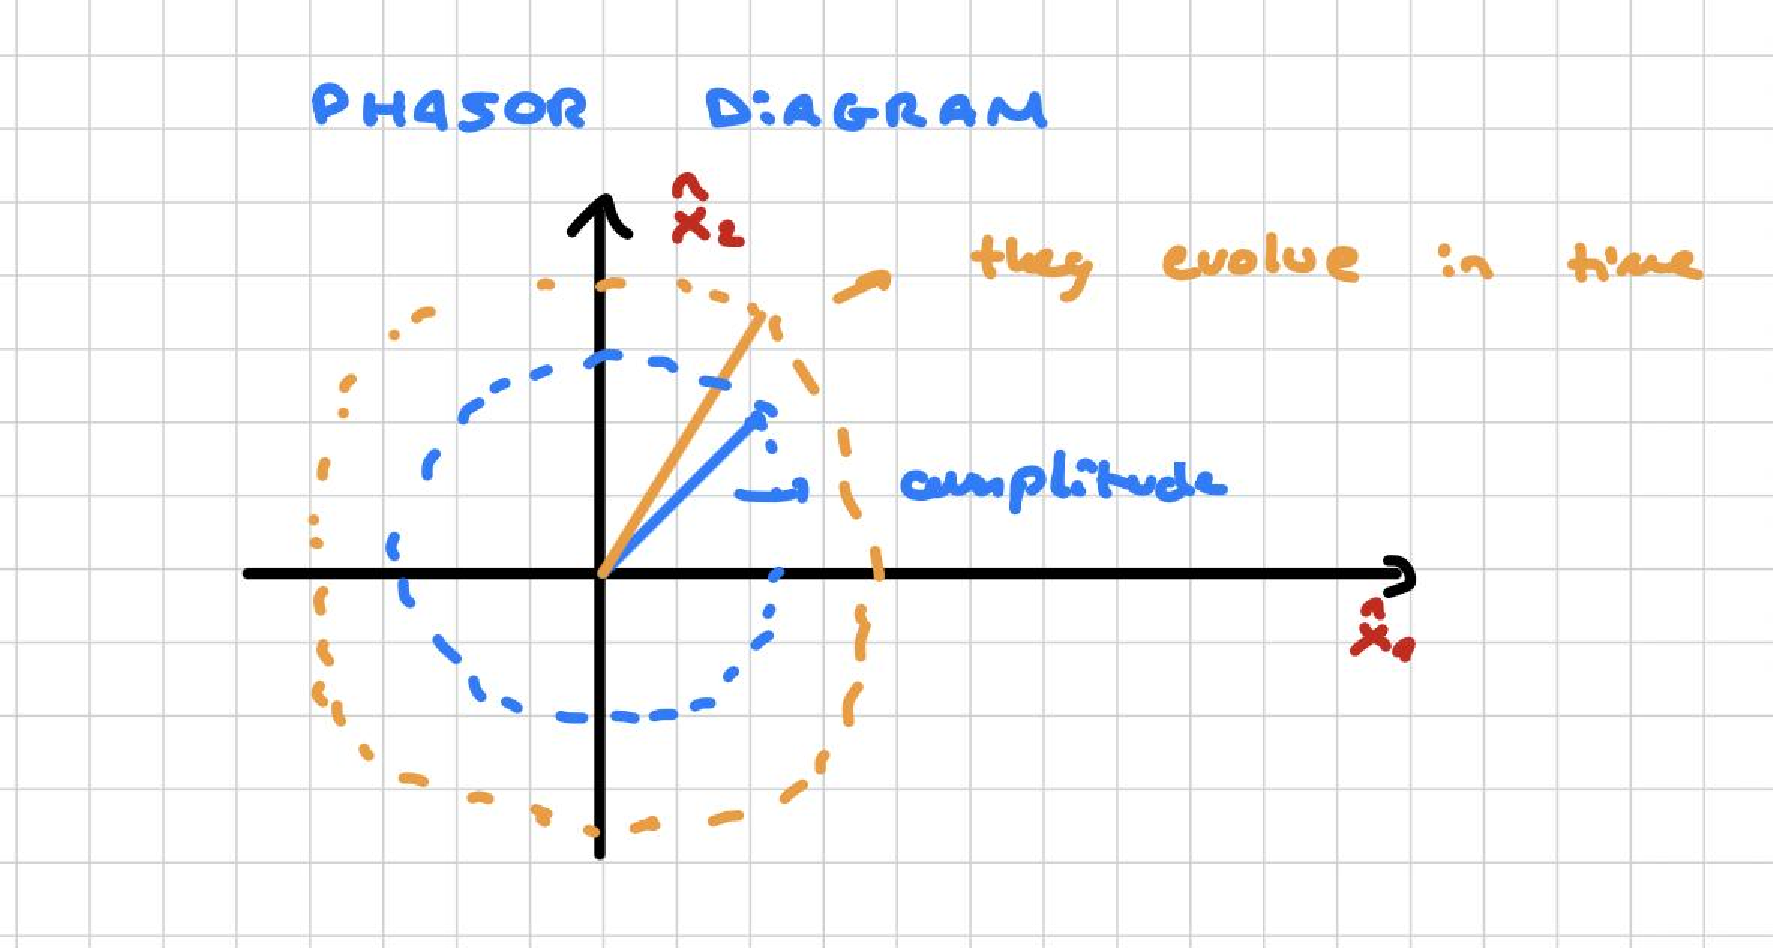
\includegraphics[width=0.6\linewidth]{images_in_pdf/11-/Grafico_66.pdf}
\end{figure}

For the \textbf{number state:}
\begin{equation}\label{eqn:11-number-state-quadratures}
\begin{split}
    \braket{n|\hat{x}_1|n} &= \braket{n|\hat{x}_2|n} =0\\\\
    \braket{n|\hat{x}_1^2|n} &= \frac{1}{4}\, \braket{n| (\hat{a}^\dagger)^2 + \hat{a}^2 + \hat{a}^\dagger\hat{a}+\hat{a}\hat{a}^\dagger|n}\\
    &=\frac{1}{4}\, (0+0+\braket{n|1+2\hat{a}^\dagger\hat{a}|n})\\
    & = \frac{1}{4}\, (1+2n) = \braket{n|\hat{x}_2^2|n} 
\end{split}
\end{equation}

This again shows that the average value of each quadrature vanishes, but the fluctuations do not. In particular, for the vacuum state, \hl{the uncertainties in quadratures operators are the same and the vacuum state, having $n=0$, minimizes the uncertainty product:}
\begin{equation}\label{eqn:11-vacuum-state-quadrature-uncertainties}
\braket{(\Delta \hat{x}_1)^2}_\text{vacuum} =\braket{(\Delta \hat{x}_2)^2}_\text{vacuum} = \frac{1}{4} 
\end{equation}

\begin{figure}[H]
    \centering
    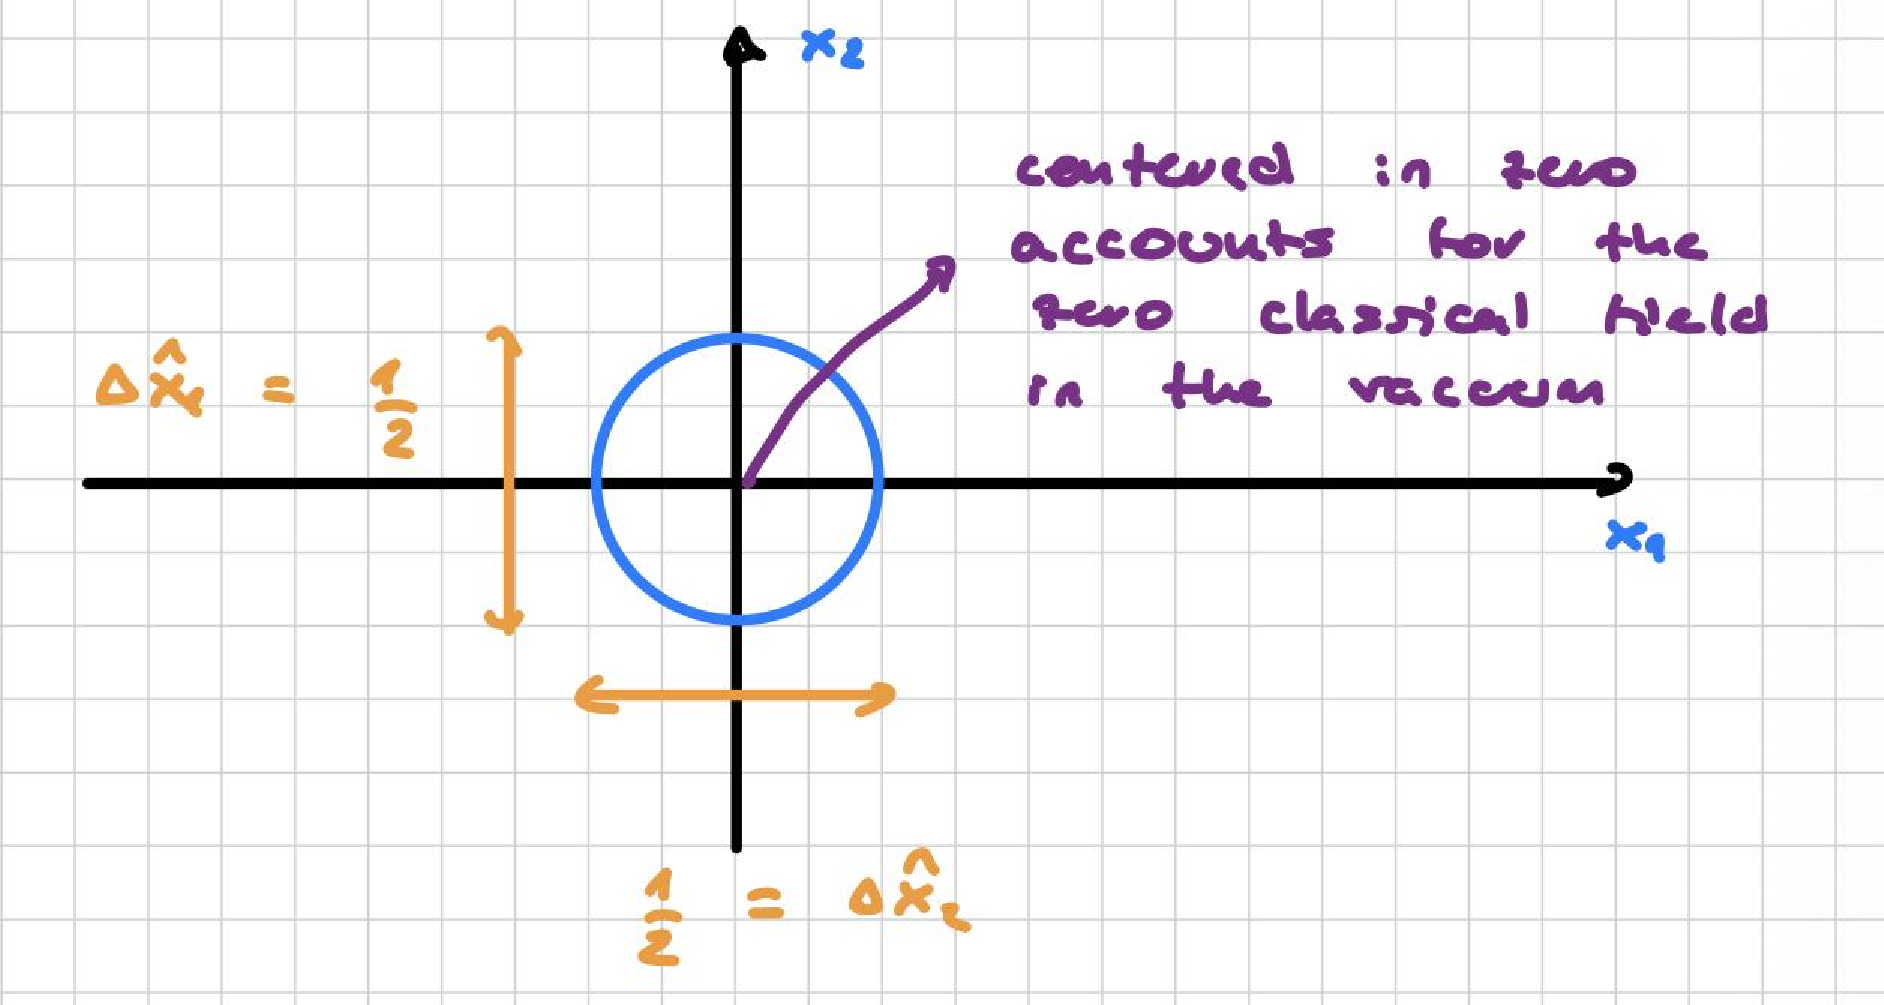
\includegraphics[width=0.6\linewidth]{images_in_pdf/11-/Grafico_67.pdf}
\end{figure}

\calloutinfo{%
States that satisfy
\begin{equation}\label{eqn:11-minimum-uncertainty-states}
\Delta \hat{x}_1\,\Delta \hat{x}_2=\frac{1}{4}
\end{equation}

are called \textbf{minimum-uncertainty states} (Eqn~\eqref{eqn:11-minimum-uncertainty-states}). The vacuum is one example, but \textbf{coherent states} also belong to this class.
}

\section{Vacuum field and Casimir Force}\label{sec:vacuum-and-casimir}

\calloutinfo{%
The vacuum field is present everywhere, even in complete absence of matter or real radiation, and it can produce observable effects. A famous manifestation is the attractive \textbf{Casimir force} between two conducting plates placed in vacuum. The physical origin of the effect is the modification of the vacuum mode structure by the cavity boundaries.
}

We suppose that:
\begin{enumerate}
    \item Outside the cavity, the vacuum energy is that of free space, with a continuous spectrum of modes.
    \begin{equation}\label{eqn:12-continuous-free-space-energy}
    E_\text{free} = \frac{\pi \hbar c}{L} \, \int_0^{\infty} m \, dm 
    \end{equation}
    
    \item Inside the cavity, the boundary conditions discretize the allowed modes, so that the vacuum energy becomes a sum over standing-wave modes.
    \begin{equation}\label{eqn:12-discrete-cavity-energy}
        E_\text{cavity} = \sum_m \hbar \omega_m = \frac{\pi\hbar c}{L} \sum_m m
    \end{equation}
    where we remembered that the mode frequencies are given by $\omega_m = m \pi c / L$ (Eqn.~\ref{eqn:11-single-mode-electric-field}).
\end{enumerate}

Since both contributions are divergent separately, only their difference is physically meaningful after regularization. For two perfectly conducting parallel plates separated by a distance $L$, we can calculate:
\[
\Delta E= E_\text{cavity}-E_\text{free} = 
\frac{\pi \hbar c}{L}\, 
\left(\sum_mm-\int m \, dm  \right) = 
 -\frac{\pi\hbar c}{12}\, \frac{1}{L}
\]

\hl{The energy decreases with the length $L$ of the cavity which means we have a \textbf{pulling force}:}
\begin{equation}\label{eqn:12-casimir-force}
    F = -\frac{\partial\Delta E}{\partial L} = -\frac{\pi \hbar c}{12}\frac{1}{L^2}
\end{equation}

If we consider all the possible polarizations:
\begin{equation}\label{eqn:12-casimir-pressure}
    P = \frac{F}{A} = -\frac{\pi^2\hbar c}{240 L^2}
\end{equation}

The negative sign shows that the force is attractive. Notice that this effect vanishes in the classical limit $\hbar\to 0$, which confirms that it is purely quantum in origin. For a separation of $L=\qty{1}{\micro\meter}$, one finds a very small pressure, of the order of
\begin{equation}\label{eqn:12-casimir-pressure-typical}
P\sim 10^{-3}\,\unit{\newton\per\meter\squared},
\end{equation}

so for an area $A=\qty{1}{\centi\meter\squared}$ the force is of order
\begin{equation}\label{eqn:12-casimir-force-typical}
F\sim 10^{-7}\,\unit{\newton}.
\end{equation}

\begin{figure}[H]
    \centering
    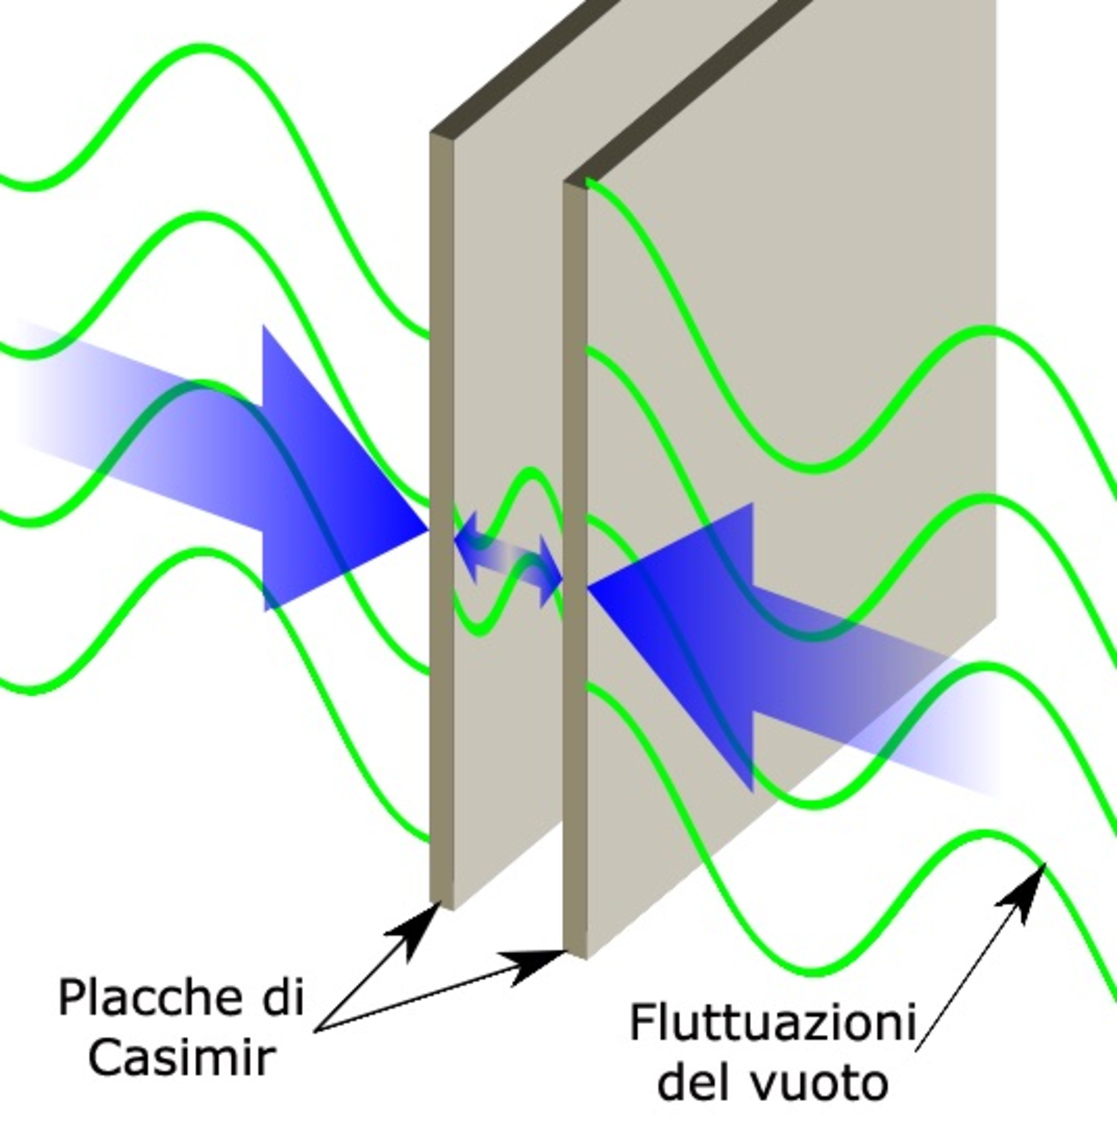
\includegraphics[width=0.4\linewidth]{images_in_pdf/12-/Effetto_Casimir.pdf}
    \caption{Schematic representation of the Casimir effect.}
\end{figure}

\calloutwarn{%
In a real lab, putting two flat plates perfectly parallel at a distance of only $1\,\mu\mathrm{m}$ without letting them touch is practically impossible. If the plates are even slightly tilted, the edges will bump into each other, short-circuiting the setup and ruining the measurement.
}

To solve this practical nightmare, experimentalists use a \textbf{sphere next to a flat plate}. 
This is done because a sphere and a plane always have exactly one single closest point, no matter how you rotate or tilt them; the alignment problem gets removed. The force is then calculated using a standard geometrical correction called the Proximity Force Approximation (PFA).

\subsubsection{Photon localizability}

Observe that photons arise as quantum excitations of the electromagnetic field, but they are also particle-like entities. This raises an important conceptual issue.

\begin{itemize}
    \item \textbf{Classical particles:} a state is fully described by instantaneous position and momentum.
    \item \textbf{Non-relativistic quantum particles:} the operators $\hat{x}$ and $\hat{p}$ do not commute, and the state is described by a wavefunction $\psi(\vec{x})=\langle \vec{x}|\psi\rangle$, which gives the probability amplitude for a position measurement.
    \item For a photon, however, the situation is different: because it is a massless spin-1 particle with gauge constraints and transversality conditions, \hl{there is no fully satisfactory position operator with all the usual properties expected for a localized particle}.
\end{itemize}
    The properties one would like for a photon position operator are:
\begin{itemize}
    \item $[\hat{x},\hat{y}]=0$;
    \item $\hat{x}$ should transform as a vector under rotations.
\end{itemize}

\calloutwarn{%
In practice, these requirements cannot be satisfied simultaneously for the photon in the same way as for massive particles. Therefore, one cannot construct a true position-space wavefunction for the photon in the usual Schrödinger sense.
    
In classical theory, Maxwell equations do not contain any particle concept. In quantum theory, photons are the quanta of the electromagnetic field and  relativistic particles by virtue of their vanishing mass, the correct description requires quantum electrodynamics rather than a single-particle Schrödinger equation.
}

\section{Coherent states}\label{sec:coherent-states}

\subsection{Summary of quadrature operators}

\hl{A coherent state is a linear superposition of number states} and this provides the closest approximation of a radiation by a laser. 

We already learned the relationship between the quadrature operators and the creation and annihilation operators:
\begin{equation}\label{eqn:13-quadratures-creation-annihilation-operators}
\begin{cases}
    \hat{x}_1 = \frac{1}{2}\, (\hat{a}+\hat{a}^\dagger ) \\
    \hat{x}_2 = \frac{i}{2}\, (\hat{a}-\hat{a}^\dagger ) 
\end{cases} \implies \hspace{2ex} \begin{cases}
    \hat{a} \hspace{0.23cm} = \hat{x}_1+i\hat{x}_2\\
    \hat{a}^\dagger  = \hat{x}_1-i\hat{x}_2
\end{cases}
\end{equation}

We are then allowed to write the Hamiltonian in terms of the quadrature operators:
\begin{equation}\label{eqn:13-hamiltonian-quadratures}
\hat{H} = \hbar \omega \left(\hat{a}^\dagger \hat{a}+\frac{1}{2}\right) =
\hbar \omega \left(\hat{x}_1^2+\hat{x}_2^2\right).
\end{equation}

We want to relay on photon number state, the basis can be used for black body radiation and chaotic light too. Remember that we have:
\begin{equation}\label{eqn:13-number-operator-eigenvalue-equation}
\hat{n}\,\ket{n} = n\, \ket{n},
\end{equation}

with uncertainty
\begin{equation}\label{eqn:13-number-operator-uncertainty}
\begin{split}
\braket{\Delta n^2} &= \braket{\hat{n}^2} - \braket{\hat{n}}^2 =\\[0.5ex]
&= \braket{n|\hat{n}\, \hat{n}|n}-(\braket{n|\hat{n}|n})^2 = \\[0.5ex]
&= n^2-n^2 = 0
\end{split}
\end{equation}

and we can write the Hamiltonian eigenvalue equation both in terms of the number operator and the quadrature operators:
\begin{equation}\label{eqn:13-hamiltonian-eigenvalue-equation}
\hat{H}\, \ket{n} = \hbar \omega \left(\hat{a}^\dagger \hat{a}+\frac{1}{2} \right)\, \ket{n} =\hbar \omega \bigl(n+\frac{1}{2}\bigr) = \hbar \omega \left(\hat{x}_1^2+\hat{x}_2^2\right)\, \ket{n}
\end{equation}

simplifying:
\begin{equation}
\left(\hat{x}_1^2+\hat{x}_2^2\right)\, \ket{n} = \left(n+\frac{1}{2}\right) \, \ket{n}
\end{equation}
\vspace{1ex}

Since the expectation values of the quadrature operators are zero $\braket{n|\hat{x}_1|n} = \braket{n|\hat{x}_2|n} = 0$, if we define the rotated quadrature operator as:
\begin{equation}\label{eqn:13-rotated-quadrature-operator}
X_\theta = \cos(\theta)\, \hat{x}_1+\sin(\theta) \, \hat{x}_2
\end{equation}

it will also have zero expectation value $\braket{n|X|n} = 0$ for any phase $\theta$. This means that the average value of the electric field is zero in a number state, and the phase is completely undefined.

A photon number state $\ket{n}$ represents an exotic state of light in sharp contrast with a classical electromagnetic wave of stable amplitude and phase. While a Fock state possesses a perfectly sharp energy (and photon number), it does not possess a classical phase analogue. In fact, a state $\ket{n}$ has a completely random phase, whereas a state with a well-defined phase must exhibit a completely broad photon number distribution. This highlights that quantum phase and photon number are complementary observables, obeying a fundamental uncertainty relation similar to position and momentum.

The vacuum state $\ket{0}$ for a single mode of frequency $\omega$ acts as the effective ground state of the system when thermal fluctuations are negligible, namely when the thermal energy is much smaller than the quantum excitation energy:
\begin{equation}\label{eqn:13-vacuum-thermal-condition}
k_B T \ll \hbar \omega.
\end{equation}

While the first excited state $\ket{1}$ (a single photon) can be generated experimentally via atomic cascade emissions or through spontaneous parametric down-conversion (SPDC), higher excited states $\ket{2}, \ket{3}, \dots$ become increasingly challenging to prepare in the laboratory.

\subsubsection{Coherent States Formalism}

A single-mode laser light operating well above threshold possesses a well-defined, stable phase. Such classical-like radiation cannot be described by a single Fock state, but corresponds to a specific linear superposition known as a \textbf{coherent state}, denoted as $\ket{\alpha}$.

Classically, we can visualize a mode being excited by an external source that shifts the electric field from zero to a finite classical amplitude $\vec{E} \propto |\alpha| \neq 0$, which in turn drives the magnetic field, generating a self-propagating harmonic wave. In the quantum framework, this process is modeled by displacing the vacuum state away from the origin of the phase space to induce an oscillating expectation value for the field.

To formalize this, we introduce the unitary \textbf{displacement operator} $\hat{D}(\alpha)$, which shifts the vacuum state by a complex amplitude $\alpha \in \mathbb{C}$:
\begin{equation}\label{eqn:13-displacement-operator-definition}
\ket{\alpha} = \hat{D}(\alpha) \ket{0}.
\end{equation}

The displacement operator is generated by the creation and annihilation operators:
\begin{equation}\label{eqn:13-displacement-operator-exponential}
\hat{D}(\alpha) = e^{\alpha \hat{a}^\dagger  - \alpha^* \hat{a}}.
\end{equation}

From its definition and the Baker-Campbell-Hausdorff lemma, $\hat{D}(\alpha)$ satisfies the following fundamental properties:
\begin{align}
\hat{D}^\dagger (\alpha) &= \hat{D}^{-1}(\alpha) = \hat{D}(-\alpha), \label{eqn:13-displacement-property-1} \\
\hat{D}^\dagger (\alpha) \hat{a} \hat{D}(\alpha) &= \hat{a} + \alpha, \label{eqn:13-displacement-property-2} \\
\hat{D}^\dagger (\alpha) \hat{a}^\dagger  \hat{D}(\alpha) &= \hat{a}^\dagger  + \alpha^*. \label{eqn:13-displacement-property-3}
\end{align}

A crucial property of the coherent state $\ket{\alpha}$ is that it is a right eigenstate of the annihilation operator $\hat{a}$. This can be proven by inserting the identity operator $\mathbb{I} = \hat{D}(\alpha)\hat{D}^\dagger (\alpha)$:
\begin{align}
\hat{D}^\dagger (\alpha) \hat{a} \ket{\alpha} &= \hat{D}^\dagger (\alpha) \hat{a} \hat{D}(\alpha) \ket{0} \nonumber \\
&= (\hat{a} + \alpha) \ket{0} = 0 + \alpha \ket{0}. \label{eqn:13-proof-eigenvalue-step1}
\end{align}

Multiplying both sides from the left by $\hat{D}(\alpha)$, we immediately find:
\begin{equation}\label{eqn:13-coherent-eigenvalue}
\hat{a} \ket{\alpha} = \alpha \ket{\alpha}.
\end{equation}

Using this eigenvalue relation, the expectation value for the photon number operator $\hat{n} = \hat{a}^\dagger  \hat{a}$ in a coherent state is easily evaluated:
\begin{equation}\label{eqn:13-coherent-mean-photons}
\braket{\alpha|\hat{n}|\alpha} = \braket{\alpha|\hat{a}^\dagger  \hat{a}|\alpha} = \alpha^* \alpha \braket{\alpha|\alpha} = |\alpha|^2 = \overline{n}.
\end{equation}

Here, $\overline{n}$ represents the mean photon number, matching the energy intensity of a classical field. However, unlike a number state, a coherent state does not contain a sharp number of photons. It is composed of an infinite superposition of Fock states:
\begin{equation}\label{eqn:13-coherent-fock-expansion}
\ket{\alpha} = \sum_{n=0}^{\infty} \ket{n} \braket{n|\alpha}.
\end{equation}

By projecting the eigenvalue equation onto $\bra{n}$ and using the property $\bra{n}\hat{a} = \sqrt{n+1}\bra{n+1}$, one finds the recurrence relation that yields the expansion coefficients:
\begin{equation}\label{eqn:13-coherent-coefficients}
\braket{n|\alpha} = \frac{\alpha^n}{\sqrt{n!}} e^{-\frac{1}{2}|\alpha|^2} \quad \implies \quad \ket{\alpha} = e^{-\frac{1}{2}|\alpha|^2} \sum_{n=0}^{\infty} \frac{\alpha^n}{\sqrt{n!}} \ket{n}.
\end{equation}

It is important to note that distinct coherent states are not orthogonal, as they are projections of shifted wave-packets that overlap in phase space:
\begin{equation}\label{eqn:13-coherent-overlap}
\braket{\alpha_1|\alpha_2} = e^{-\frac{1}{2}|\alpha_1|^2 - \frac{1}{2}|\alpha_2|^2} \sum_{n=0}^{\infty} \frac{(\alpha_1^* \alpha_2)^n}{n!} = e^{-\frac{1}{2}|\alpha_1|^2 - \frac{1}{2}|\alpha_2|^2 + \alpha_1^* \alpha_2}.
\end{equation}

The physical overlap probability (the profile indistinguishability) is given by the absolute square:
\begin{equation}\label{eqn:13-coherent-overlap-squared}
|\braket{\alpha_1|\alpha_2}|^2 = e^{-|\alpha_1 - \alpha_2|^2}.
\end{equation}

Hence, coherent states are only approximately orthogonal when their complex amplitudes are significantly different, i.e., when $|\alpha_1 - \alpha_2| \gg 1$.

To compute the variance of the photon number, $(\Delta n)^2 = \braket{\hat{n}^2} - \overline{n}^2$, we expand the operator $\hat{n}^2$ using the commutation relation $[\hat{a}, \hat{a}^\dagger ] = 1$ to reorder it into a normal-ordered form:
\begin{equation}\label{eqn:13-normal-ordering-n2}
\hat{n}^2 = \hat{a}^\dagger  \hat{a} \hat{a}^\dagger  \hat{a} = \hat{a}^\dagger  ( \hat{a}^\dagger  \hat{a} + 1 ) \hat{a} = \hat{a}^\dagger  \hat{a}^\dagger  \hat{a} \hat{a} + \hat{a}^\dagger  \hat{a}.
\end{equation}
Taking the expectation value with respect to $\ket{\alpha}$ yields:
\begin{equation}\label{eqn:13-n2-expectation}
\braket{\alpha|\hat{n}^2|\alpha} = \braket{\alpha|\hat{a}^\dagger  \hat{a}^\dagger  \hat{a} \hat{a}|\alpha} + \braket{\alpha|\hat{a}^\dagger  \hat{a}|\alpha} = |\alpha|^4 + |\alpha|^2 = \overline{n}^2 + \overline{n}.
\end{equation}
Substituting this back into the variance definition, we obtain:
\begin{equation}\label{eqn:13-photon-variance-final}
(\Delta n)^2 = (\overline{n}^2 + \overline{n}) - \overline{n}^2 = \overline{n}.
\end{equation}

\hl{This identity, where the variance equals the mean ($(\Delta n)^2 = \overline{n}$), is the signature of a quantum \textbf{Poissonian process}}.

Indeed, the probability $P(n)$ of detecting exactly $n$ photons in a coherent state field matches the photon number distribution:
\begin{equation}\label{eqn:13-poisson-distribution}
P(n) = |\braket{n|\alpha}|^2 = \left| e^{-\frac{1}{2}|\alpha|^2} \frac{\alpha^n}{\sqrt{n!}} \right|^2 = e^{-|\alpha|^2} \frac{(|\alpha|^2)^n}{n!} = e^{-\overline{n}} \frac{\overline{n}^n}{n!}.
\end{equation}

This confirms that photocounting statistics of ideal laser light are fully governed by a Poisson distribution with mean intensity $\overline{n}$.

The fractional uncertainty in the number of photons in the coherent state is:
\[\frac{\Delta n}{\overline{n}} = \frac{\sqrt{\overline{n}}}{\overline{n}} =\frac{1}{\sqrt{\overline{n}}}\]
as a matter of course, it decreases with increase in the number mean photon $\overline{n}$.

\calloutinfo{%
The coherent states $\ket{\alpha}$ are quantum states close to the classical ones:
\begin{enumerate}
    \item The expectation value of the $\vec{E}$ has the form of a classical field;
    \item The fluctuations in the $\vec{E}$ variables are the same as for the vacuum;
    \item The fluctuations in the fractional uncertainty decreases with increasing the average photon number. This lead us to classical limit where variance of a stable wave vanishes.
    \item The states become well localized in phase with increasing of photon number.
\end{enumerate}
}

\callout{A coherent state can be represented with a phasor of length $|\alpha|$ and angle $\theta$.}{%
Since
\begin{equation}
\begin{cases}
    \hat{x}_1 = \sqrt{\tfrac{m\omega}{2\hbar}}\, \hat{q} =
    \frac{1}{2}(\hat{a}+\hat{a}^\dagger )\\
    \hat{x}_2 = \sqrt{2m\hbar \omega}\, \hat{p} = 
    \tfrac{1}{2i}(\hat{a}-\hat{a}^\dagger )
\end{cases}
\end{equation}

we shall write:
\begin{equation}\label{eqn:13-alpha-polar-form}
    \alpha = |\alpha|\, e^{i\theta}
\end{equation}
\begin{proof}
\begin{equation}\label{eqn:13-alpha-polar-form-proof}
    \begin{split}
    \braket{\alpha|\hat{x}_1|\alpha} = \frac{1}{2}\braket{\alpha|(\hat{a}^\dagger +\hat{a})|\alpha} = \frac{1}{2}(\alpha^*+\alpha) \\
    &\hspace{2.35cm}= \Re(\alpha) = |\alpha|\, \cos(\theta)\\\\
    \braket{\alpha|\hat{x}_2|\alpha} = \frac{1}{2}i\braket{\alpha|(\hat{a}^\dagger -\hat{a})|\alpha} = \frac{1}{2}(\alpha^*+\alpha) \\
    &\hspace{2.35cm}= \Im(\alpha) = |\alpha|\, \sin(\theta)\\
    \end{split}
\end{equation}
\end{proof}
}
\vspace{1ex}

If we use:
\[\begin{cases}
    \hat{x}_1^2 = \frac{1}{4}(\hat{a}^\dagger \hat{a}+2\hat{a}^\dagger \hat{a}+\hat{a}\hat{a}+1)\\[1ex]
    \hat{x}_2^2 = \frac{1}{4}(-\hat{a}^\dagger \hat{a}+2\hat{a}^\dagger \hat{a}-\hat{a}\hat{a}+1)
\end{cases}\]

It can be proven that:
\[(\Delta \hat{x}_1)^2 = (\Delta \hat{x}_2)^2 = \frac{1}{4}\]

In contrast to the variances for the number state, \hl{the coherent state is a \textbf{quadrature-minimum uncertainty state} for all mean photon numbers $\overline{n} =|\alpha|^2$}.
The mean field amplitude associated with the coherent state is an arrow of length $|\alpha| = \sqrt{\overline{n}}$ inclined at an angle $\theta$ to the real axis.
\begin{figure}[H]
        \centering
        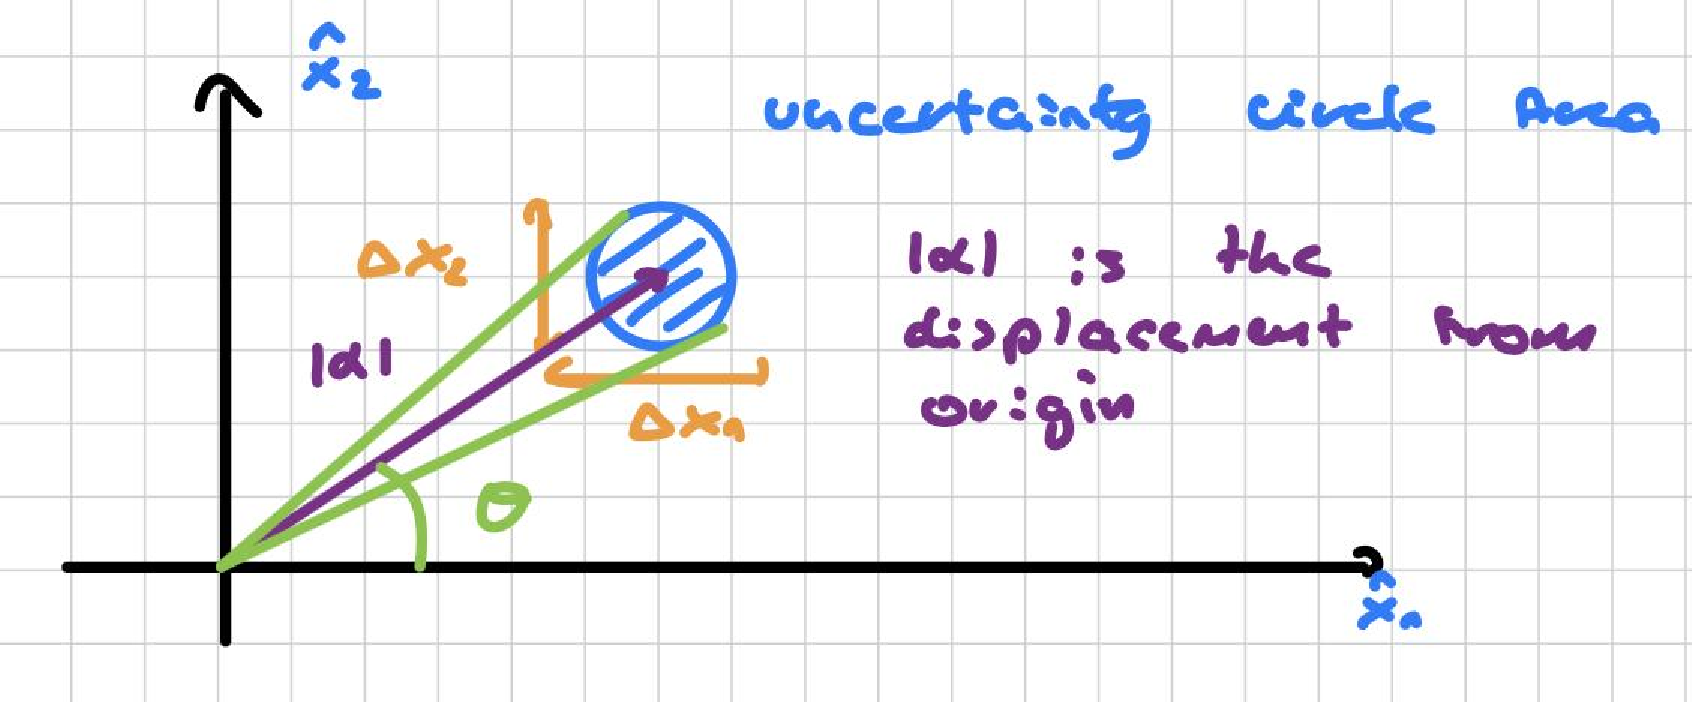
\includegraphics[width=0.6\linewidth]{images_in_pdf/13-/Grafico_68.pdf}
    \end{figure}

$|\alpha|^2$ and $\theta$ are uncertain, in contrast with the classical wave where these quantities are well known.

The length of the phasor is between $\alpha+\frac{1}{4}$ and $\alpha-\frac{1}{4}$:
\[ 
\begin{split}
    \Delta n &= \bigl(\sqrt{\overline{n}}+\frac{1}{4}\bigr)^2-\bigl(\sqrt{\overline{n}}-\frac{1}{4}\bigr)^2 \\
    &=\bigl(|\alpha|+\frac{1}{4}\bigr)^2-\bigl(|\alpha|-\frac{1}{4}\bigr)^2 \\
    &= |\alpha| = \sqrt{\overline{n}}
\end{split}
\]

\subsubsection{The shot-noise in optical detection is a result of quantum nature of light}

$\Delta \theta$ subtended by the diameter of the disk at origin. If $|\alpha| >> 1$ the arc rule gives:
\[\Delta\theta \approx \frac{\text{uncertainty diameter}}{|\alpha|} =\frac{\frac{1}{2}}{|\alpha|} = \frac{1}{2\sqrt{\overline{n}}}\]
We can calculate:
\[\Delta n \, \Delta \theta = \sqrt{\overline{n}}\, \frac{1}{2\sqrt{\overline{n}}} = \frac{1}{2}\]

This is a form of an uncertainty relation, but obtained by geometrical argument. So $\frac{\Delta \overline{n}}{\overline{n}}$ and $\Delta \theta$ vary like $\frac{1}{\alpha}$. When $\overline{n}$ increases, the E.M. waves becomes better defined both in amplitude and phase and lead us to the classical wave limit.

So what we see is:
\begin{itemize}
    \item \textbf{Coherent states $\ket{\alpha}$}:
    Fluctuation are equal in every direction (circle).
    \begin{figure}[H]
        \centering
        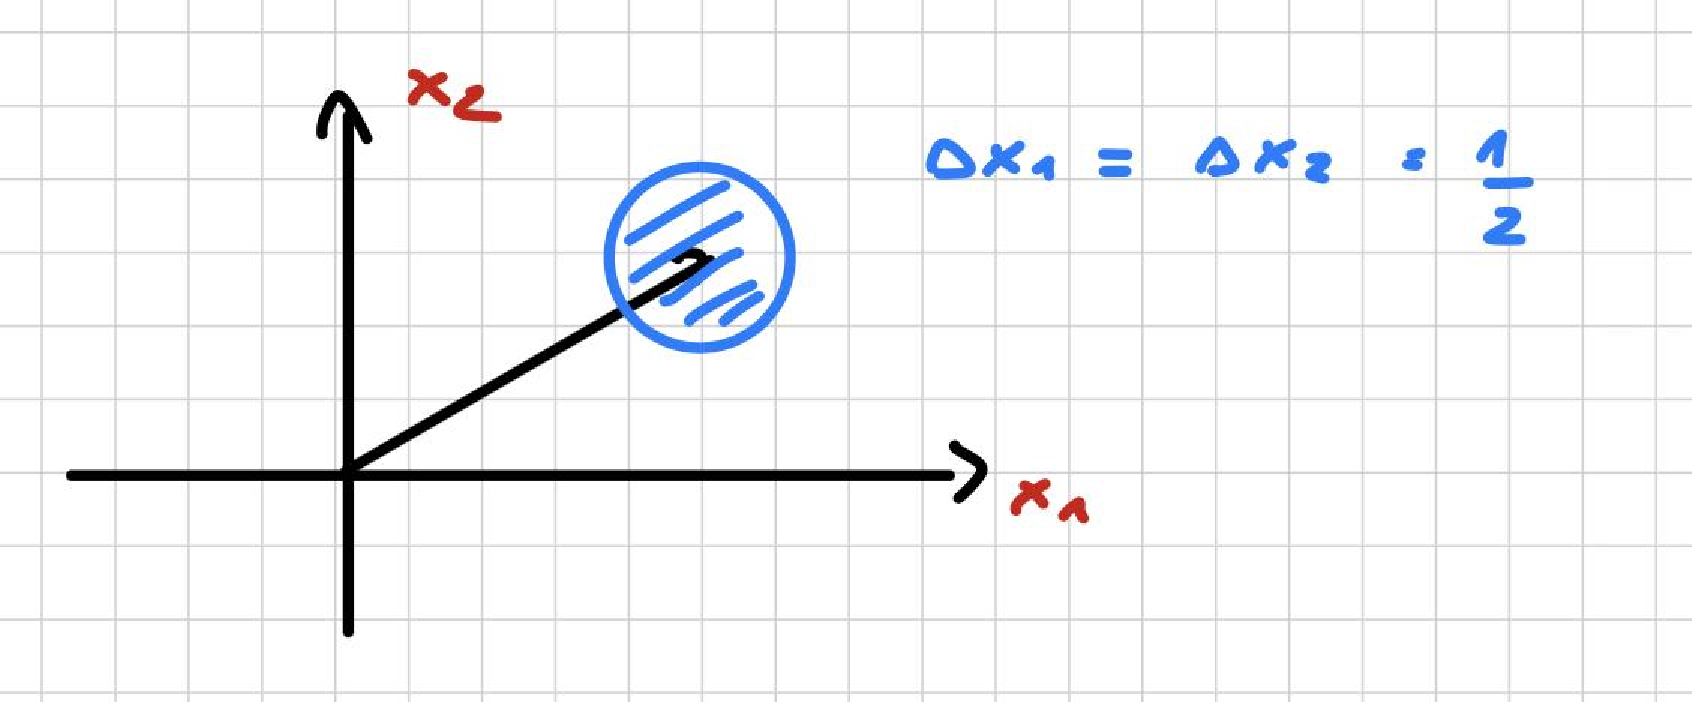
\includegraphics[width=0.6\linewidth]{images_in_pdf/13-/Grafico_69.pdf}
    \end{figure}

    Center is at distance $|\alpha| = \sqrt{\overline{n}}$ at angle $\theta$ above x-axis.
    
    \item \textbf{Vacuum state $\ket{0}$}: 
    Fluctuation are equal in every direction(circle.)
    \begin{figure}[H]
        \centering
        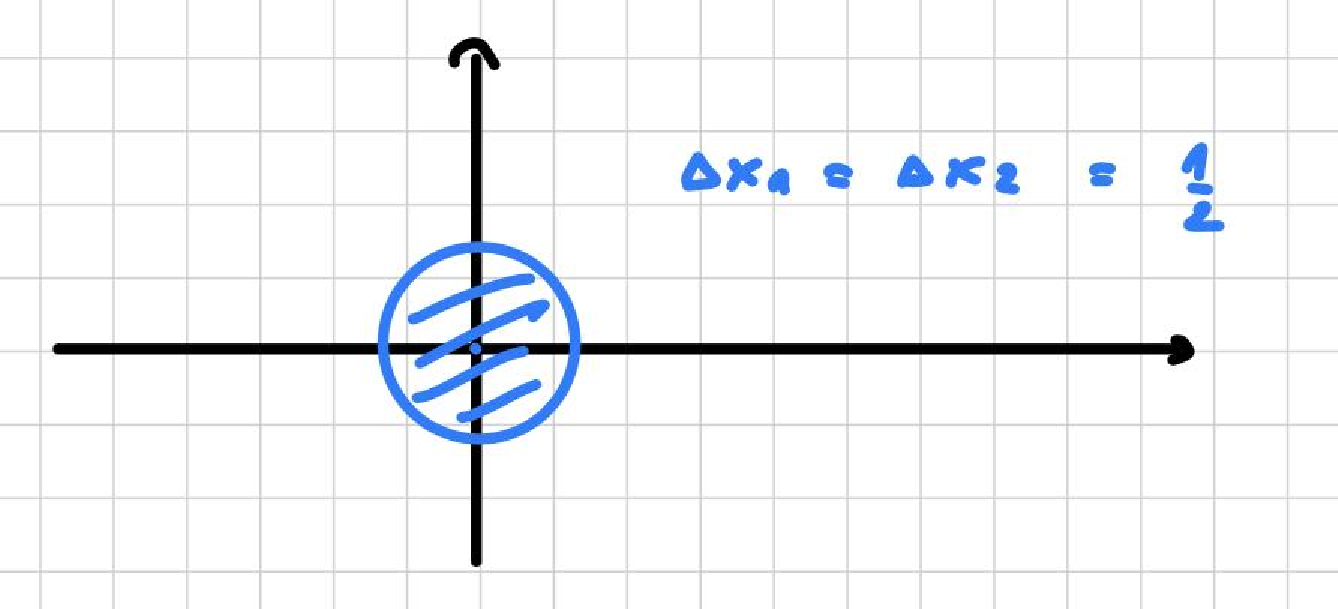
\includegraphics[width=0.6\linewidth]{images_in_pdf/13-/Grafico_70.pdf}
    \end{figure}

    $|\alpha |= 0$ and $\Delta \theta$ is large as possible $\Delta \theta = 2\pi$
    
    \textbf{Number state $\ket{n}$}: 
    We have a circle of radius $n$.
    \begin{figure}[H]
        \centering
        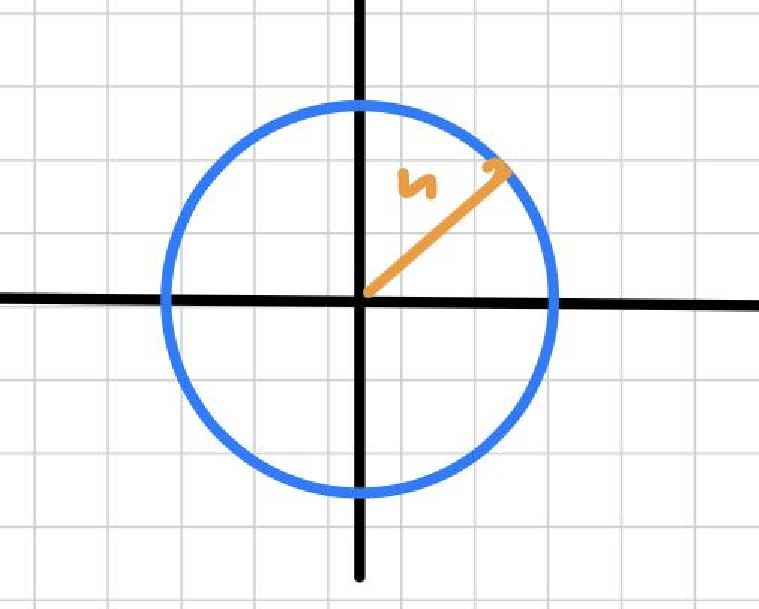
\includegraphics[width=0.6\linewidth]{images_in_pdf/13-/Grafico_71.pdf}
    \end{figure}

    $\Delta n = 0$, we know the number of photons, $\Delta \theta = 2\pi$  is max 
\end{itemize}
We recall the operator:
\[\begin{cases}
    \hat{E}_x =A_0 (\hat{a}+\hat{a}^\dagger )\sin(kz)\\
    \hat{x}_1 = \frac{1}{2}(\hat{a}+\hat{a}^\dagger ) 
\end{cases} \implies\hat{E}_x = 2A_0\, \sin(kz) \, \hat{x}_1 \]
Let us consider the time evolution of a quantum state for not interacting field:
\[\begin{split}
    &\ket{\alpha} \to \ket{\alpha e^{-i\omega t}}\\
    \implies &\bra{\alpha e^{-i\omega t}} \hat{x}_1 \ket{\alpha e^{-i\omega t}} = \alpha\,  \cos(\omega t)\\
    \implies &\bra{\alpha e^{-i\omega t}} \hat{x}_2 \ket{\alpha e^{-i\omega t}} = -\alpha\,  \sin(\omega t)\\
\end{split}\]
In the phasor diagram that means a clockwise rotation of the circle. 
\begin{figure}[H]
        \centering
        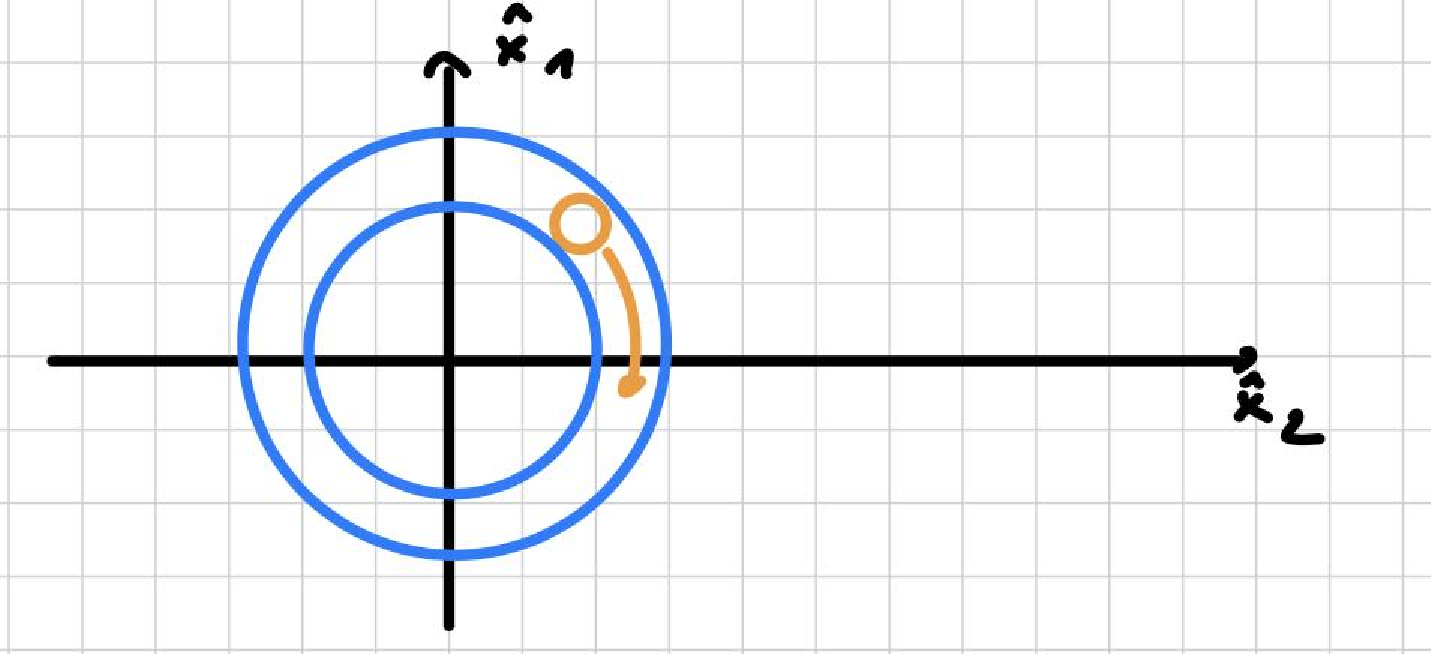
\includegraphics[width=0.6\linewidth]{images_in_pdf/13-/Grafico_72.pdf}
    \end{figure}

\[  \bra{\alpha e^{-i\omega t}} \hat{E}_x \ket{\alpha e^{-i\omega t}} = 2A_0\,  \sin(\omega t) \, \braket{\hat{x}_1} = 2A_0\,  \sin(\omega t) \, \alpha \, \cos(\omega t) \]
The time evolution is the projection of the $\braket{\hat{x}_1}$ axis as a function of the time.
\begin{figure}[H]
    \centering
    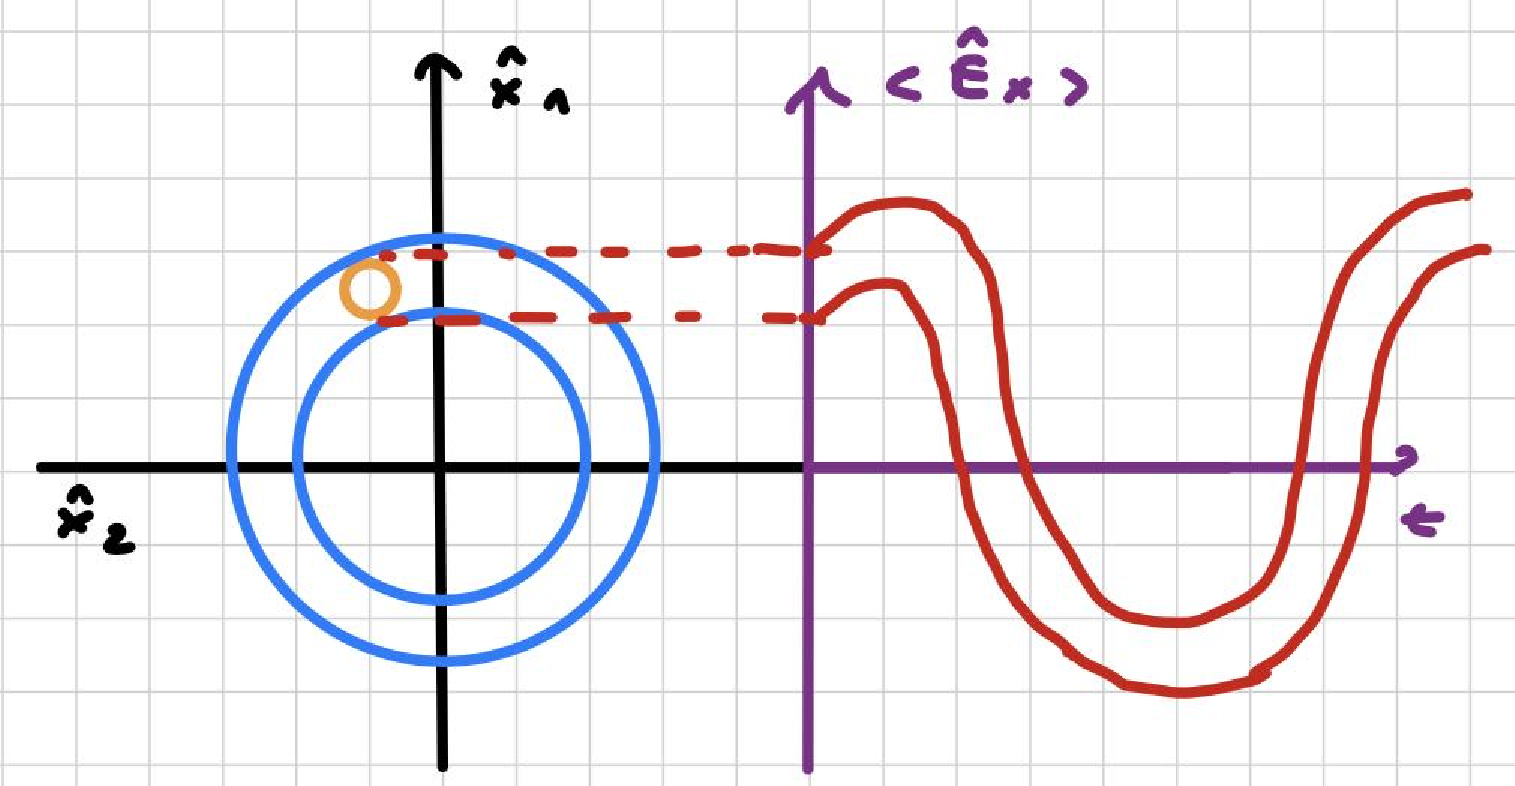
\includegraphics[width=0.6\linewidth]{images_in_pdf/13-/Grafico_73.pdf}
\end{figure}

Notice that the greater is the field $\braket{\hat{E}_x} \propto \alpha$, more the field appears classical. Coherent state is the most classical of all the quantum states, the expectation value of field must be very different from the classical ones. In case of number state $\braket{\hat{E}_x} = $.  However we will see that there are states with expectation value different from zero, but the fluctuations are less than a coherent state in one part of the field. These kind of states are called $\textbf{SQUEEZED STATES}$.

\subsubsection{Squeezed states}

We have other minimum uncertainty states with: 
\[\Delta x_1^2 < \frac{1}{4} \hspace{1cm} \text{or} \hspace{1cm} \Delta x_2^2 > \frac{1}{4}\]
This means that we have less noise in one of the quadrature operators, the circle is \textbf{squeezed} into an ellipse of the same area: 
\begin{figure}[H]
        \centering
        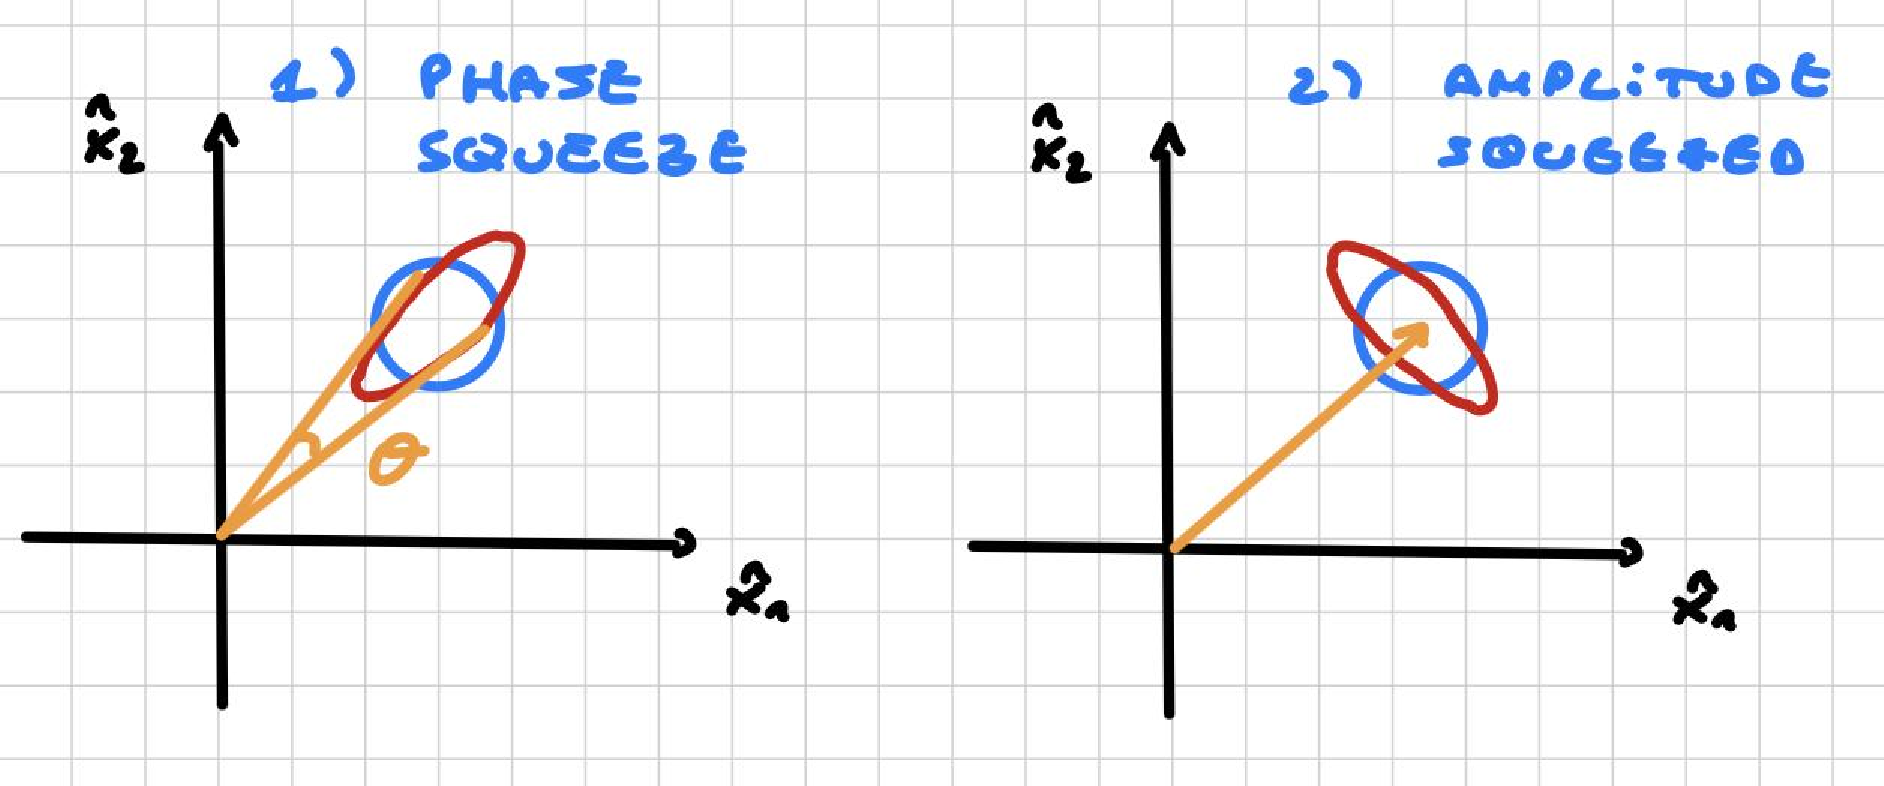
\includegraphics[width=0.6\linewidth]{images_in_pdf/13-/Grafico_74.pdf}
    \end{figure}

While coherent state have poissonian photon number distribution and shot-noise, \textbf{the amplitude-squeezed light will have sub-poissonian statistics with a noise level below the shot-noise.}

These states are represented by $(\alpha,\epsilon)$ with $\epsilon = r_s \, e^{i2\theta_s}$, where:
\begin{itemize}
    \item $|\alpha|^2$ is the intensity of the state.
    \item $\theta_s$ is the orientation of the squeezing axis.
    \item$r_s$ is the degree of squeezing, $\epsilon = 0$ for a coherent state.
\end{itemize}

We can generate a squeezed state starting from a vacuum state:
\[ \ket{\alpha,\epsilon} = \hat{D}(\alpha) \, \hat{S}(\epsilon) \, \ket{0}\]
Where we define the \textbf{squeezing operator}:
\begin{equation}\label{eqn:13-squeezing-operator}
    \hat{S}(\epsilon) = 
    \exp{
        \left(
            \frac{1}{2}\epsilon^*\hat{a}^2-\frac{1}{2}\epsilon \hat{a}^\dagger 
        \right)}
\end{equation}

We can compute:
\begin{align}\label{eqn:13-squeezed-state-expectation-values}
    &\bra{\alpha,\epsilon} \hat{a} \ket{\alpha,\epsilon} = \alpha\\[0.5ex]
    &\bra{\alpha,\epsilon} \hat{a}^2 \ket{\alpha,\epsilon} = \alpha^2-\cosh(r_s)\, \sinh(r_s)\, e^{2i\theta_s}\\[0.5ex]
    &\bra{\alpha,\epsilon} \hat{a}^\dagger \hat{a} \ket{\alpha,\epsilon} = |\alpha|^2+\sinh^2(r_s)
\end{align}

The coherent state are obtained for $r_s \to 0$, while the vacuum states are obtained for $\alpha \to 0$.

We can define the rotated quadrature operators for vacuum state:
\begin{equation}\label{eqn:13-rotated-quadrature-operator-squeezed}
\left(
\begin{matrix}
    \hat{y}_1\\[0.5ex]
    \hat{y_2}
\end{matrix}
\right) = 
\left(
\begin{matrix}
    \cos (\tfrac{\theta}{2}) &\sin(\tfrac{\theta}{2})\\[0.5ex]
    -\sin(\tfrac{\theta}{2}) &\cos(\tfrac{\theta}{2})
\end{matrix} 
\right)
\, 
\left(
\begin{matrix}
    \hat{x}_1\\[0.5ex]
    \hat{x}_2
\end{matrix}
\right)
\end{equation}

Or:
\[\hat{y}_1+i\hat{y}_2 = (\hat{x}_1+\hat{x}_2)\, e^{-i\frac{\theta}{2}}\]
The variances should be:
\[\begin{cases}
    \Delta \hat{y}_1^2 = \frac{1}{4}e^{-2r_s}\\[0.5ex]
    \Delta \hat{y}_2^2 = \frac{1}{4}e^{+2r_s}
\end{cases}\]

\begin{figure}[H]
    \centering
    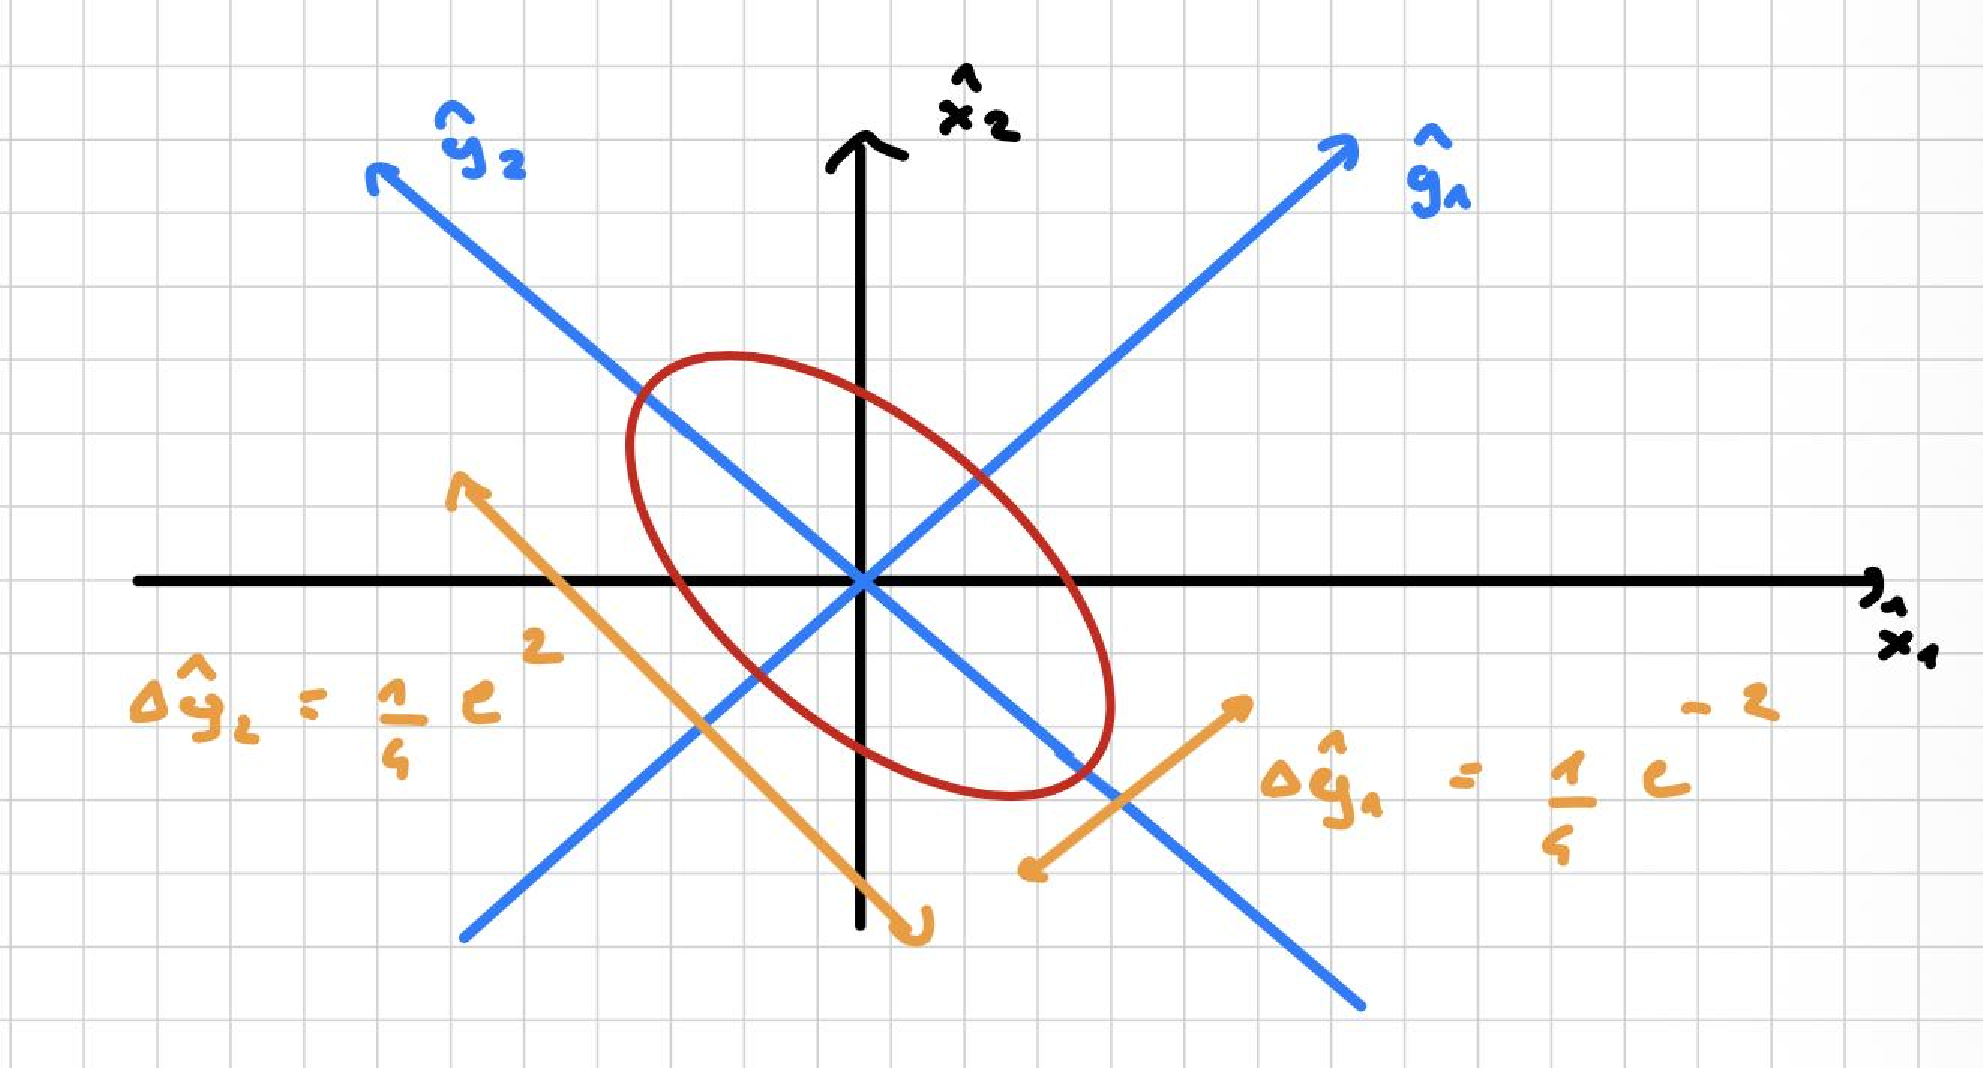
\includegraphics[width=0.6\linewidth]{images_in_pdf/13-/Grafico_75.pdf}
\end{figure}

For a generic squeeze state $\ket{\alpha,\epsilon}$, we have:
\[\braket{\hat{y}_1+i\hat{y}_2} = \alpha e^{-i\frac{\theta}{2}}\]
\begin{figure}[H]
        \centering
        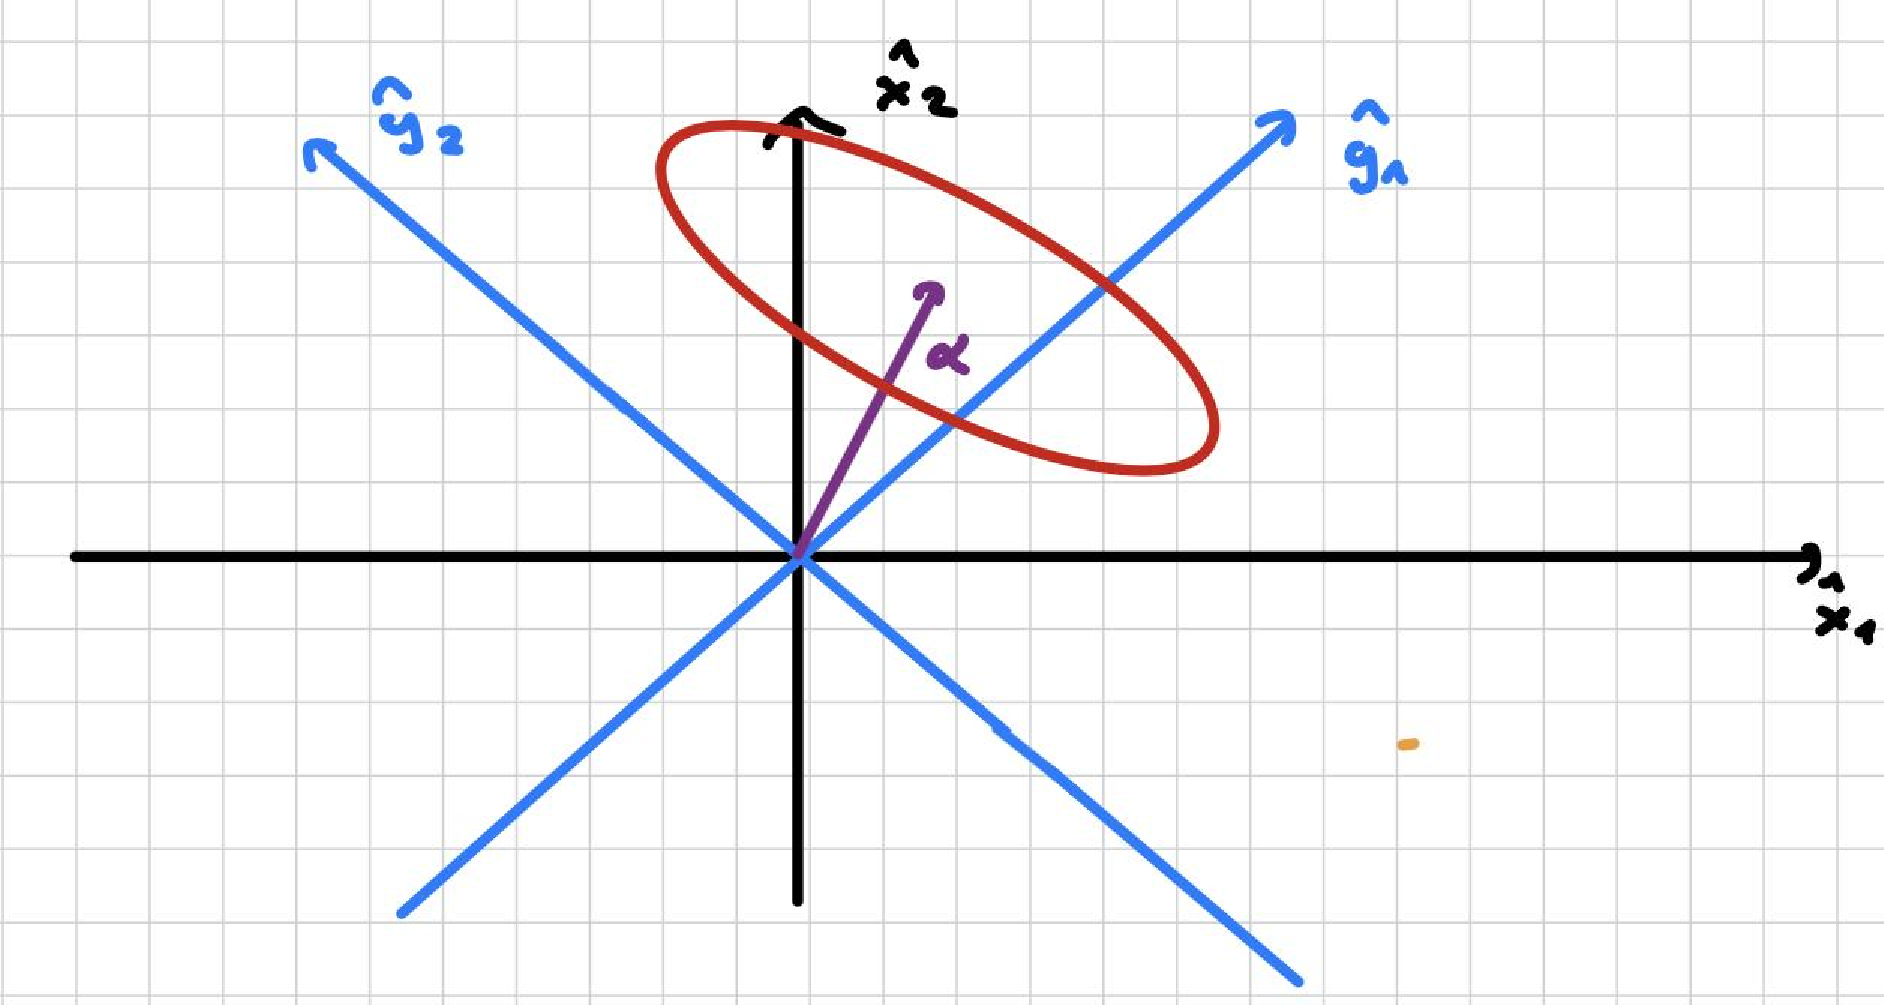
\includegraphics[width=0.6\linewidth]{images_in_pdf/13-/Grafico_76.pdf}
\end{figure}

Error ellipse is the same as for the squeeze vacuum, although displaced by $\alpha$. If we consider the single mode $\hat{E}$:
\[
\hat{E}(t) = A_0 \sin(kz)\bigl(\hat{a}e^{-i\omega t}+\hat{a}^\dagger e^{i\omega t}\bigr)
\]

Where: 
\begin{itemize}
    \item $\omega t = $ phase of the field.
    \item $\hat{a},\hat{a}^\dagger =$ operators at $t=0$. 
\end{itemize}

If we set $x = \omega t$ and look at the Equation~\ref{eqn:11-electric-field-quadrature-operators}:
\begin{equation*}
\hat{E}(x)= 2A_0\, \sin(kz) [\hat{x}_1\, \cos(x) + \hat{x}_2 \, \sin(x)]
\end{equation*}

From the fact that:
\begin{equation}\label{eqn:13-commutation-relation-quadratures}
\bigl[\hat{x}_1,\hat{x}_2\bigr] = \frac{i}{2}
\end{equation}

 we obtain:
\begin{equation}\label{eqn:13-commutation-relation-electric-field}
\left[\hat{E}(x=0) ,\hat{E}(x)\right] = i A_0^2 \, \sin^2(kz)\, \sin(x)
\end{equation}

\hl{Operators at different phases don't commute!}

\callout{Proof of the commutation relation between $\hat{E}(x=0)$ and $\hat{E}(x)$.}{%
\begin{proof}
Let's start by evaluating the field at $x=0$:
\begin{equation}\label{eqn:13-electric-field-x0}
\hat{E}(x=0) = 2 A_0 \sin(kz)\, \hat{x}_1
\end{equation}

Next, we compute the actual commutator:
\begin{equation}\label{eqn:13-electric-field-commutator-proof}
\begin{split}
\left[
    \hat{E}(0), \hat{E}(x)
\right] &= 
\left(2 A_0\, \sin(kz)\right)^2 
\bigl[
    \hat{x}_1, \hat{x}_1 \cos(x) + \hat{x}_2 \sin(x)
\bigr] = \\[0.5ex]
&= 4 A_0^2 \, \sin^2(kz)
\bigl[
    \hat{x}_1, \hat{x}_2 \sin(x)
\bigr] = \\[0.5ex]
&= 4 A_0^2 \, \sin^2(kz) \sin(x) \bigl[
    \hat{x}_1, \hat{x}_2
\bigr]
\end{split}
\end{equation}

where we have used the fact that $\hat{x}_1$ commutes with itself and that $\sin(x)$ is a scalar factor. Substituting the commutation relation in Eqn.~\ref{eqn:13-commutation-relation-quadratures} into the above expression, the result is proven.
\end{proof}
}

If the uncertainty in the field at $x=0$ is:
\[\Delta \hat{E}(0) < \frac{1}{\sqrt{2}}A_0\,|\sin(kz)\, \sin(x)|\]
Then at some other phases we must have:
\[\Delta \hat{E}(x) > \frac{1}{\sqrt{2}} A_0\, |\sin(kz)\, \sin(x)|\]

\calloutinfo{%
    Squeeze light contains phase-dependent noise that is reduced below that of the vacuum for some phases and enhanced above that of the vacuum for others.
}

Distribution of noise in the $\vec{E}$ for squeezed states is:
\begin{figure}[H]
        \centering
        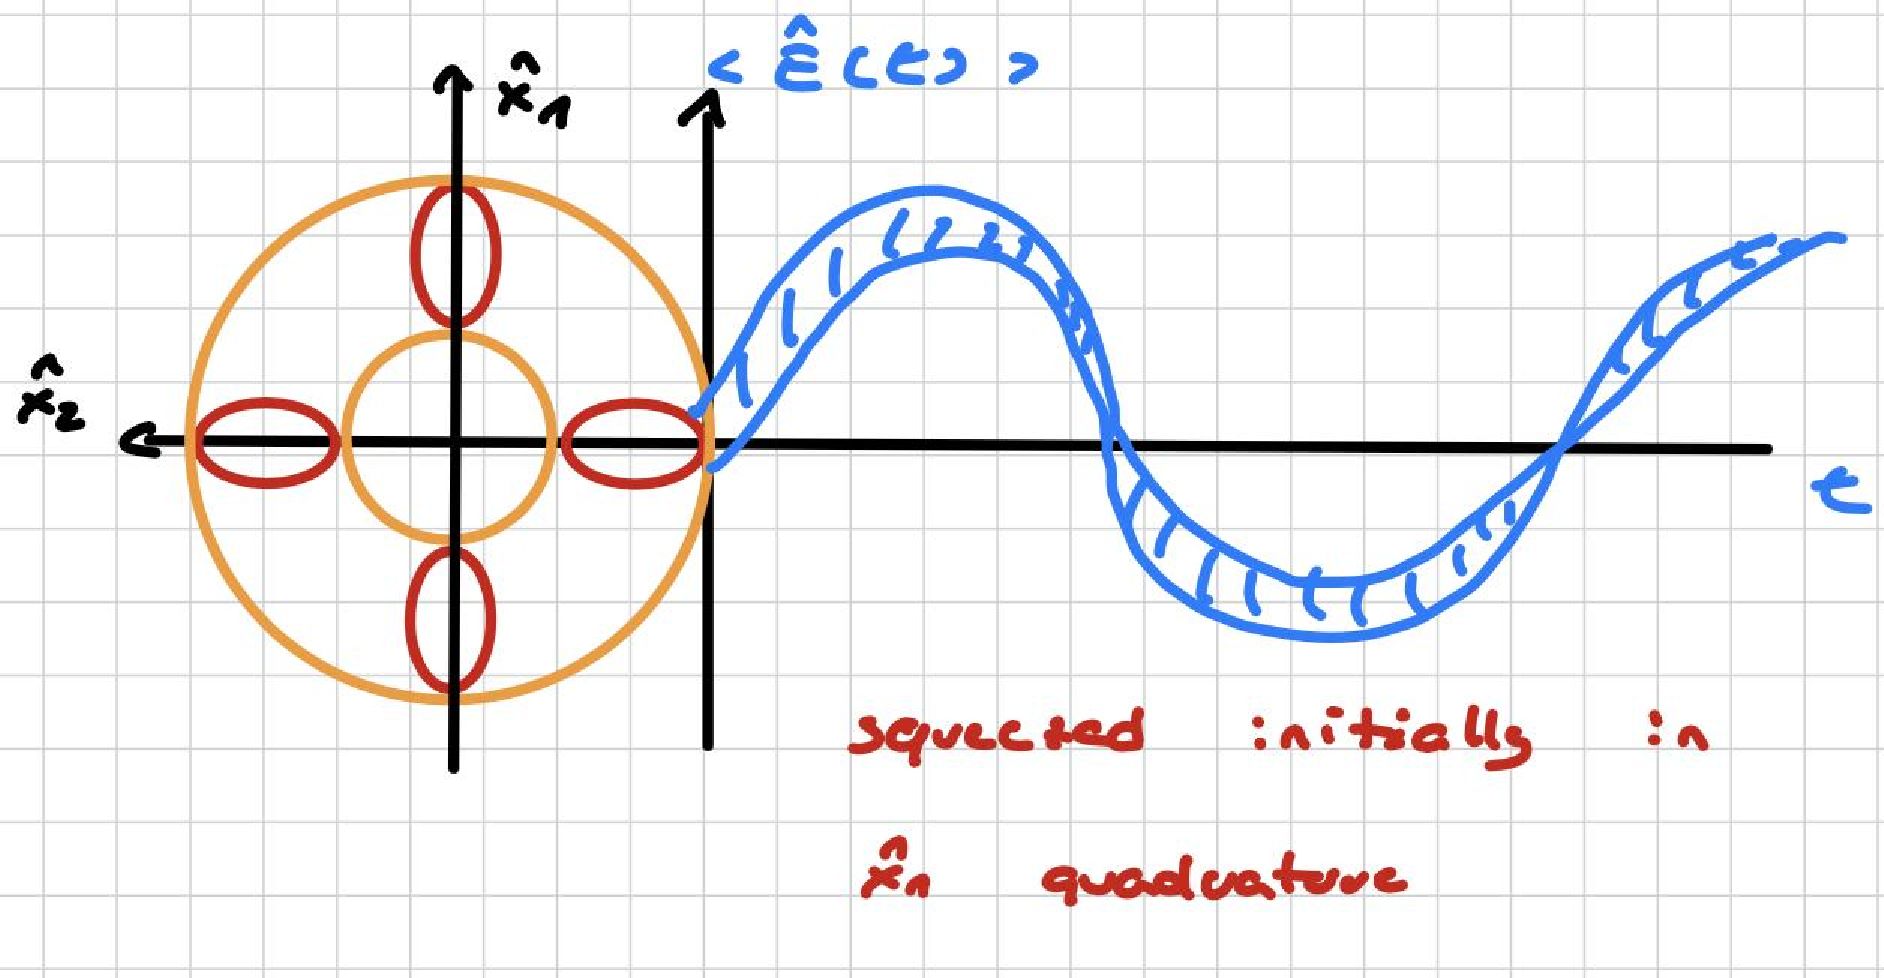
\includegraphics[width=0.6\linewidth]{images_in_pdf/13-/Grafico_77.pdf}
        \caption{}
    \end{figure}
\begin{figure}[H]
        \centering
        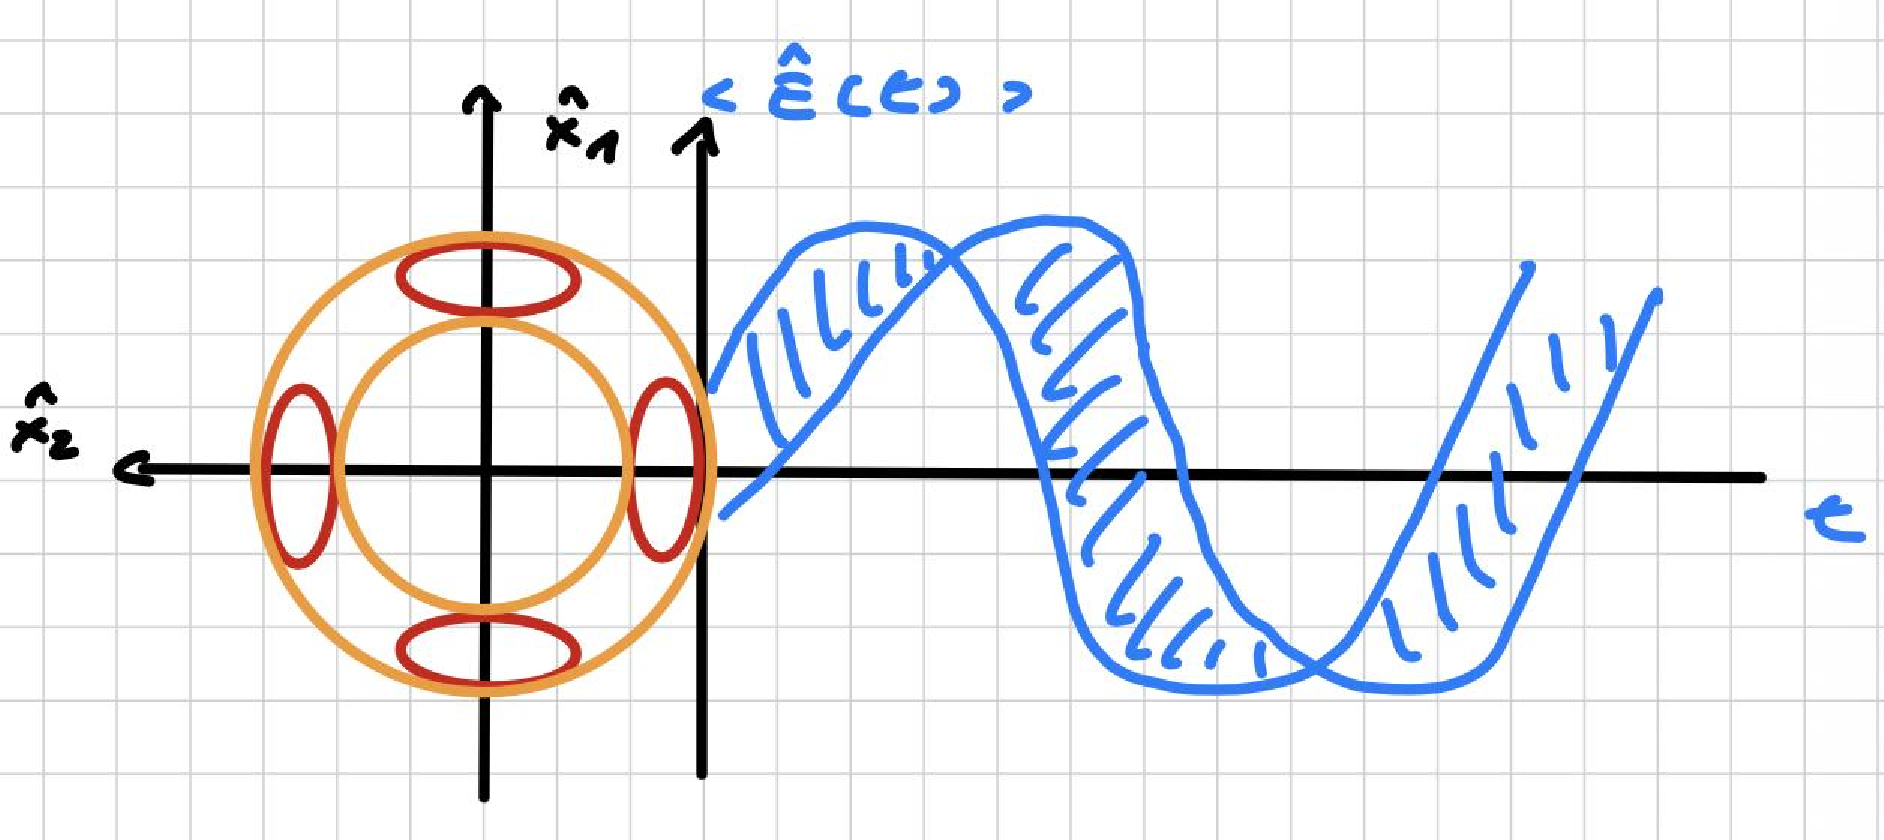
\includegraphics[width=0.6\linewidth]{images_in_pdf/13-/Grafico_78.pdf}
        \caption{}
    \end{figure}

It can be shown that:

\begin{table}[H]
\label{tab:squeezed-states}
  \centering
  \begin{tabular}{|c|c|c|}
    \hline
      & Amplitude squeezing &  Phase squeezing \\\\
    \hline
    $\Delta n$ & $\sqrt{\overline{n}}\cdot e^{-r_s}$ & $\sqrt{\overline{n}}\cdot e^{+r_s}$\\\\
    \hline
    $\Delta \theta$ & $\frac{1}{2\sqrt{\overline{n}}}\cdot e^{+r_s}$ & $\frac{1}{2\sqrt{\overline{n}}}\cdot e^{-r_s}$\\
  \end{tabular}
\end{table}

This means that $\Delta n_{A.S.} < \Delta n = \sqrt{\overline{n}}$ and $\Delta \theta_{P.S.} < \Delta \theta$, \textbf{the photon number fluctuation are sub-poissonian in a squeezed state.}

\section{Detection of quadrature-squeezed vacuum states}\label{sec:vacuum-states-detection}
Suppose that a light field is sent onto a $50:50$ beam splitter, while a second strong field, called the \textbf{local oscillator} (LO), enters the other input port. The LO has a large amplitude but the same optical frequency as the signal field. The two output beams are detected by two photodetectors, and the resulting photocurrents are subtracted by a differential electronics stage. This configuration is called \textbf{balanced homodyne detection}. 
\begin{figure}[H]
    \centering
    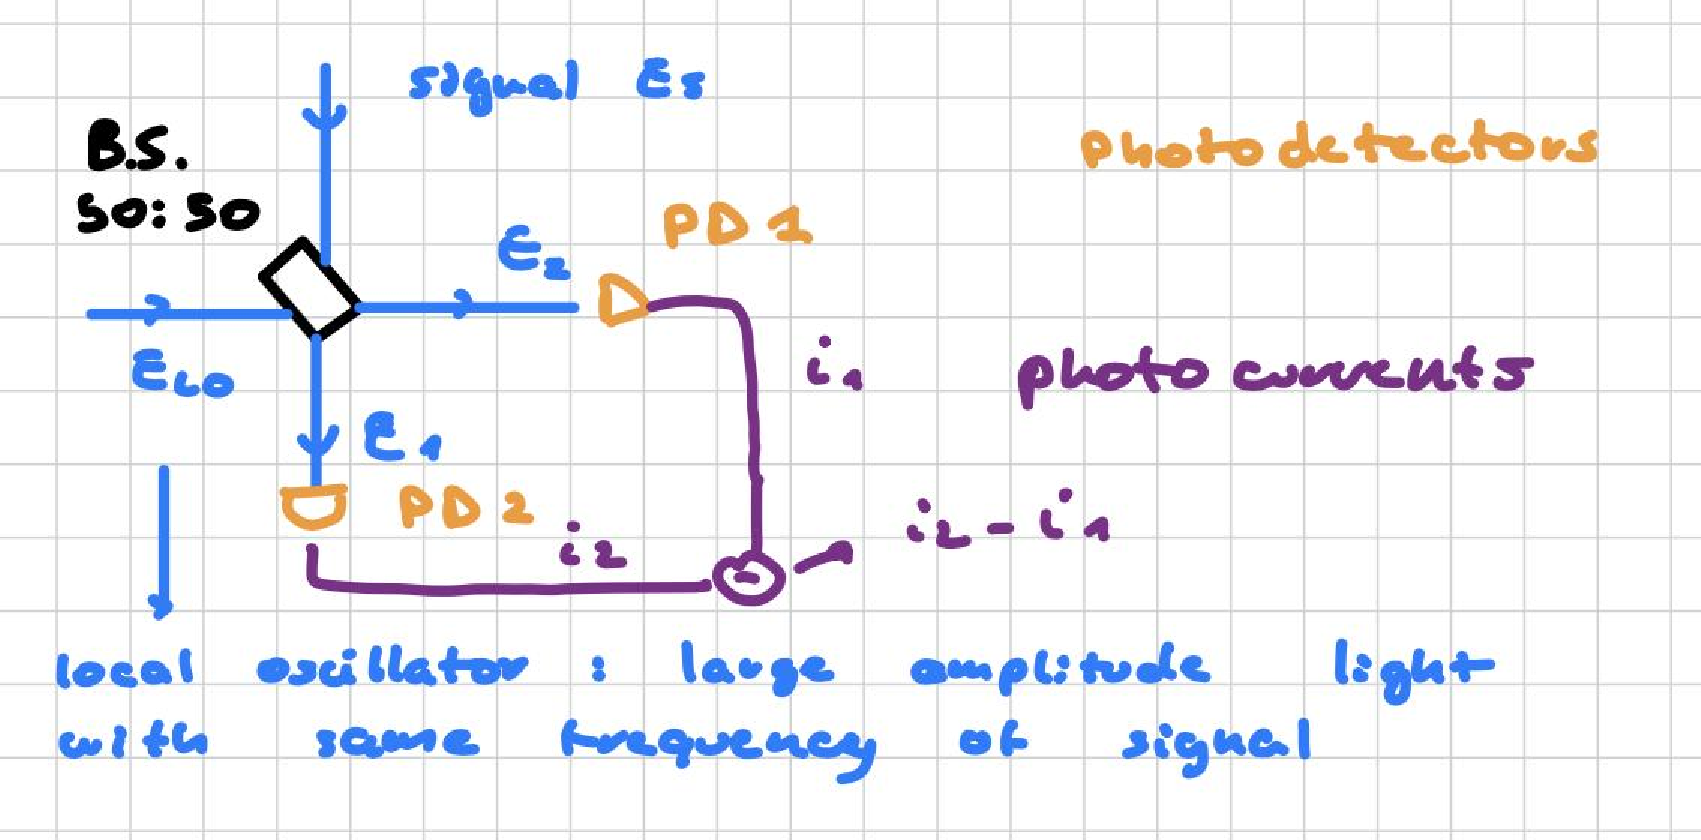
\includegraphics[width=0.6\linewidth]{images_in_pdf/14-/Grafico_79.pdf}
\end{figure}

We can distinguish two different situations:
\begin{enumerate}
    \item \textbf{No input at the signal port:} the local oscillator is equally split between the two detectors, so classically one expects
    \[
    i_2-i_1=0.
    \]
    However, because photons arrive randomly, each photodetector sees independent Poissonian fluctuations. Subtracting the two photocurrents removes the average signal, but it does not remove the quantum fluctuations, so the output still contains shot noise. For an ideal setup, the balanced detector has the same shot-noise level as a single detector measuring the same total optical power.
    \item \textbf{A signal field $E_s$ is present:}
    \[
    E_1=\frac{1}{\sqrt{2}}\left(E_{LO}e^{i\theta_{LO}}+E_s\right),
    \qquad
    E_2=\frac{1}{\sqrt{2}}\left(E_{LO}e^{i\theta_{LO}}-E_s\right).
    \]
    The local oscillator is a strong field and can therefore be treated classically, whereas the signal field is weak and must be treated quantum mechanically. We can decompose it into quadrature components:
    \[
    E_s=E_s^{x_1}+iE_s^{x_2}.
    \]
    Then the two output fields can be written as
    \[
    E_1=\frac{1}{\sqrt{2}}\Big[(E_{LO}\cos\theta_{LO}+E_s^{x_1})
    +i(E_{LO}\sin\theta_{LO}+E_s^{x_2})\Big],
    \]
    \[
    E_2=\frac{1}{\sqrt{2}}\Big[(E_{LO}\cos\theta_{LO}-E_s^{x_1})
    +i(E_{LO}\sin\theta_{LO}-E_s^{x_2})\Big].
    \]
    Since the photocurrent is proportional to $|E|^2$, the differential output is
    \[
    i_2-i_1 \propto E_1E_1^*-E_2E_2^*
    \propto E_{LO}\Big[\cos(\theta_{LO})\,E_s^{x_1}
    +\sin(\theta_{LO})\,E_s^{x_2}\Big].
    \]
    Therefore:
    \begin{itemize}
        \item if $\theta_{LO}=0,\pi,2\pi,\dots$, the output is proportional to the amplitude quadrature $E_s^{x_1}$;
        \item if $\theta_{LO}=\frac{\pi}{2},\frac{3\pi}{2},\dots$, the output is proportional to the phase quadrature $E_s^{x_2}$.
    \end{itemize}
    In this way, \textbf{the balanced homodyne detector measures the signal quadrature that is in phase with the local oscillator.}
\end{enumerate}
Let us reconsider the case with no signal at the input port. In that case, vacuum modes enter the signal port and the output is proportional to
\[
i_2-i_1 \propto E_{LO}\,E_{\mathrm{vac}}.
\]
In the absence of a signal, the balanced homodyne detector measures the vacuum fluctuations, which set the shot-noise level. In this wiew the detector can be viewed as homodyning the local oscillator with the vacuum field. \\\\
For a squeezed vacuum state instead, one quadrature has reduced noise below this limit, while the orthogonal quadrature has increased noise. This reduction below shot noise cannot be explained classically. But \textbf{how can we genrate these states?}\\\\
Quadrature-squeezed states can be generated by nonlinear optics.\\\\
Suppose that a nonlinear crystal is pumped by an intense laser beam with frequency
\[
\omega_p=2\omega,
\]
while a weak seed field has frequency
\[
\omega_s=\omega.
\]
This is the \textbf{degenerate parametric amplifier} configuration:
\begin{figure}[H]
    \centering
    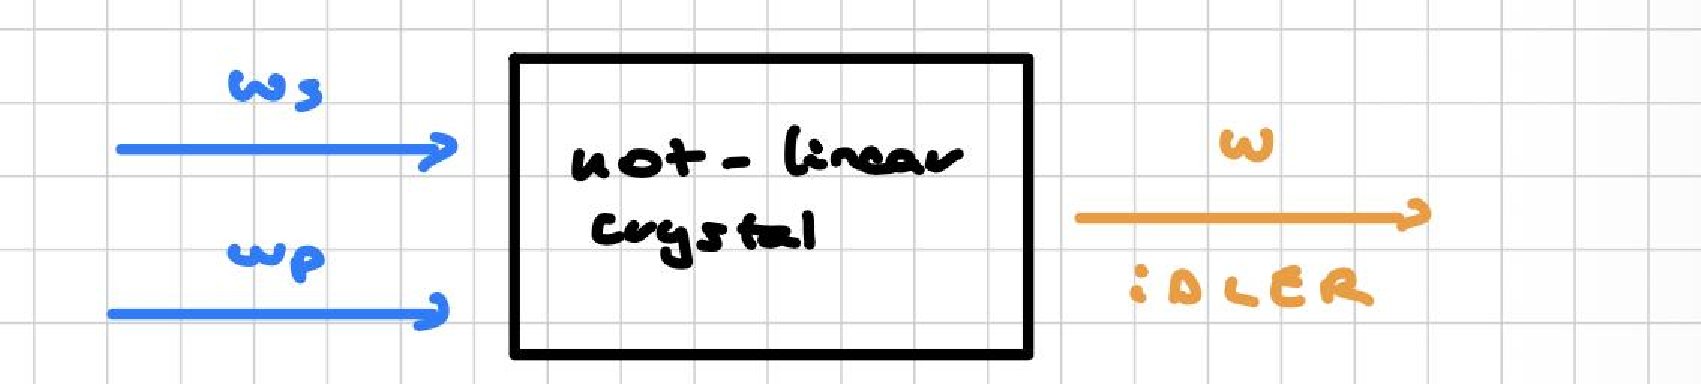
\includegraphics[width=0.6\linewidth]{images_in_pdf/14-/Grafico_80.pdf}
\end{figure}

In the degenerate case, the signal and idler fields have the same frequency:
\[
\omega_i=\omega_p-\omega_s=\omega.
\]
The nonlinear crystal mixes the pump and the signal through a $\chi^{(2)}$ interaction, so that the amplification of the field depends on the relative phase between the input signal and the pump. In the degenerate case, this phase-sensitive process can either amplify or deamplify a given field quadrature. If no signal is injected, the crystal acts on the vacuum field and converts vacuum fluctuations into a \textbf{squeezed vacuum} state.\\\\
In the absence of a seed, the only input at the signal port is the vacuum field, whose average amplitude is zero but whose fluctuations are not:
\[
E_{\mathrm{vac}} \sim \sqrt{\frac{\hbar\omega}{2\epsilon_0 V}}.
\]
\begin{figure}[H]
    \centering
    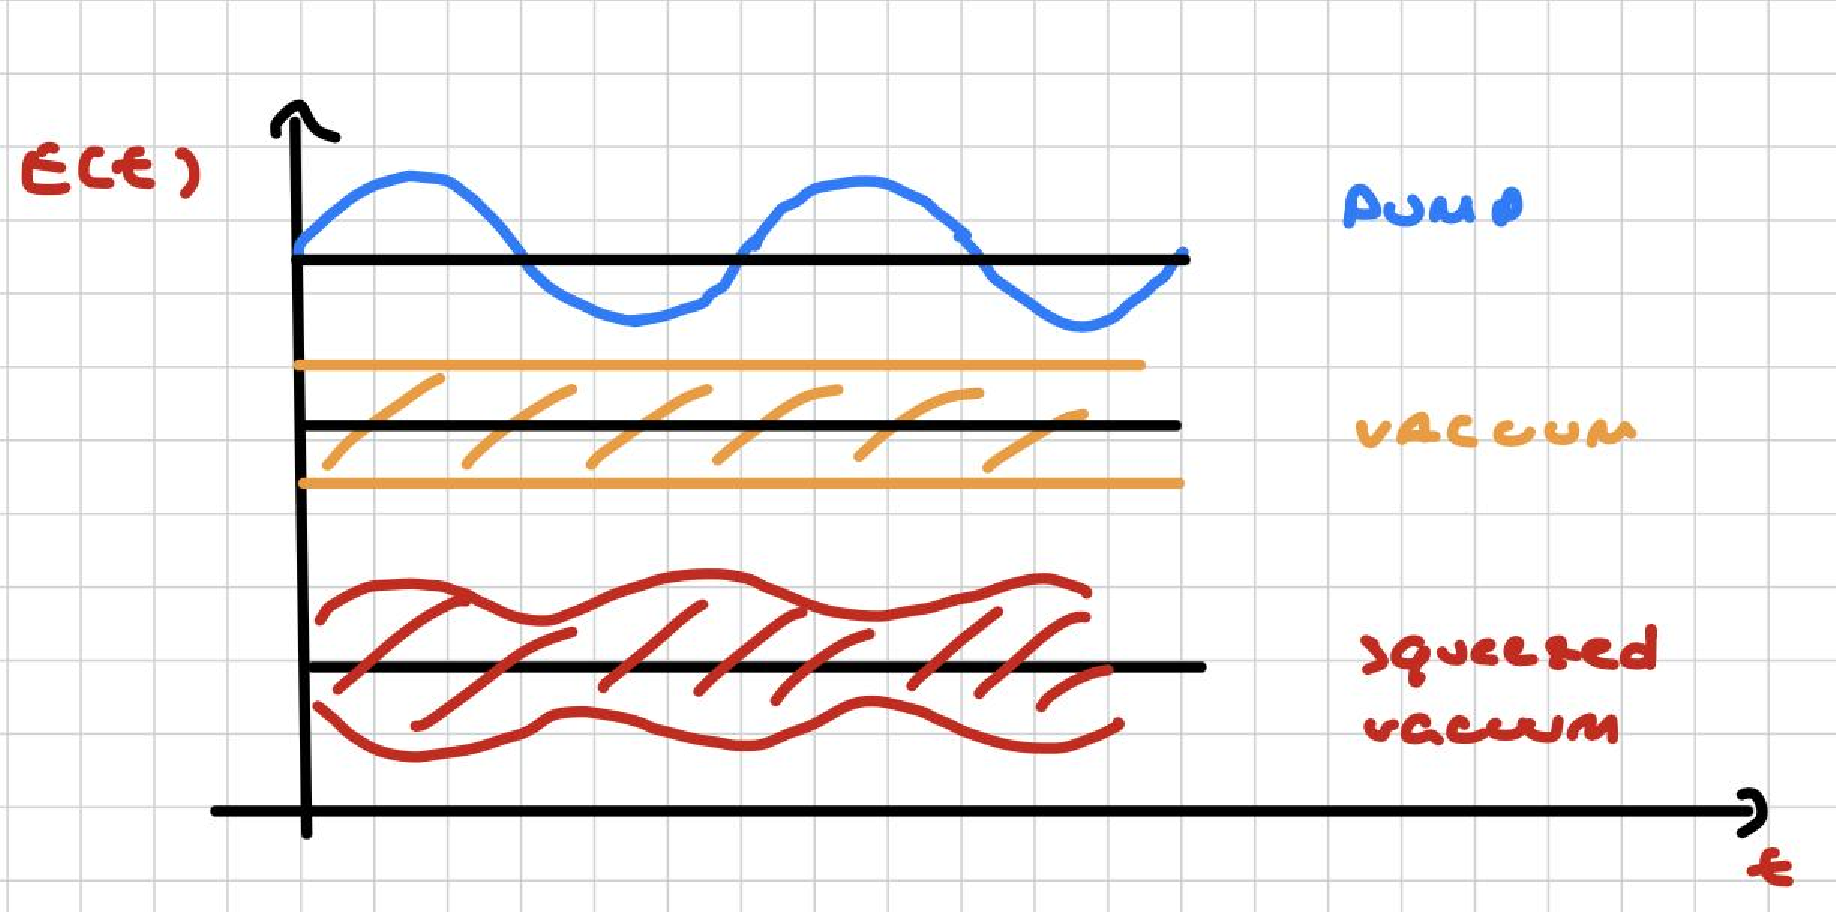
\includegraphics[width=0.6\linewidth]{images_in_pdf/14-/Grafico_81.pdf}
\end{figure}

\textbf{By changing the phase we can modulate the squeeze vacuum states and beat the shot noise:} Changing of phase correspond to select different field quadratures in the balanced homodyne detector. As result, one can observe either reduced noise below the shot-noise limit in the squeezed quadrature or increased noise above it in the conjugate quadrature $\implies$ the quantum noise is redistributed between two complementary quadratures. \\\\
This is the basic principle of squeezed-light metrology and is crucial in ultra-sensitive experiments, such as gravitational-wave detection, where reducing quantum noise is essential.

\section{Quantum entanglement}\label{sec:quantum-entanglement}
The fundamental goal is to use entangled states to conduct optical test of Q.M., but we need to have single photons in order to conduct interference experiments and teleportation.
In Q.M. the observables follow a probability distribution and unless a system is in a eigenvalue of the observable, all we can do is to predict the probability with a particular eigenvalue when the measurement is repeated several times on identically prepared systems.

This means that making a measurement \textbf{doesn't reveal a pre-existing value of the observable}. The act of measurement makes the wave function collapse in a way that is not certain.

Suppose to prepare a photon as bit 1 in $\ket{V}$ state, a measurement of the diagonal component $\ket{D_+}$ with a beam splitter could return the value $+1$ (transmission) or $-1$ (reflection) with equal probability $50 \%$.
Until the measurement is made it simply doesn't have a well defined value of the diagonal component. This reflect the \textbf{orthodox view of Q.M.}

Instead, the \textbf{realist position} consider the Q.M. as an incomplete theory requiring some other unknown information to complete the description of the physical system. This lead to the \textbf{Hidden variables theory and EPR paradox 1935}.
\subsection{EPR-B}
Now we discuss a simplified version of EPR proposed by Bohm:

Let us assume to have  a source that emits photon pairs having \textbf{correlated polarizations}, if one is $\ket{H}$ the other one will be $\ket{V}$. We can describe it with the following form:
\begin{equation}\label{eqn:15-entangled-state-example}
\ket{\psi} = \frac{1}{\sqrt{2}} \,  \bigl(\ket{H,V}-\ket{V,H}\bigr)
\end{equation}

the photons are indistinguishable, each on can be equally $\ket{H}$ and $\ket{V}$. This configuration is a classic example of an \textbf{entangled state:} a name reserved to states that cannot be expressed as tensor product states $\ket{H}\otimes  \ket{V}$.

Suppose two photons are emitted in opposite directions, then we place a B.S. and a photodetector at $10$ m far from the source and measure one of the photons and obtain $\ket{H}$. We immediately know -- even at any arbitrary distance -- that the other photon measurement, performed by a trusted friend of us, will get $\ket{V}$.

In the \say{realist} point of view: the distant photon our friend measured was always $\ket{V}$, since the moment it was emitted. Instead, in the \say{orthodox} point of view: the measurement collapses the wave function and produces instantaneously the state $\ket{H}$ for one photon and $\ket{V}$ for the other one. This seems to contradict the relativistic principle: information can't travel faster than light.

% / / / / / / / / / / / / / / / / / / / / / / / / / / / / / / / / / / / / / / / /
% / / / / / / / / / / / / / / / / / / / / / / / / / / / / / / / / / / / / / / / /

\callouterror{%
\subsection{Bell experiment}
Allowed two polarizers to be independently adjusted (da capire). We have a polarizer A with $\vec{n}_A$ orientation and a polarizer B with $\vec{n}_B$ orientation. He proposed to compute the average of the product of the polarizations for a given pair of correlated photons and polarizers  orientation.

According to Q.M.
\[P(\vec{n}_A,\vec{n}_B) = -\vec{n}_A\cdot\vec{n}_B\]

Bell demonstrate that this result is incompatible with any local hidden variable theory. If we suppose to have a third polarizer $\vec{n}_C$, it is possible to derive the \textbf{Bell inequality}
\[
|P(\vec{n}_A,\vec{n}_B)-P(\vec{n}_A,\vec{n}_C)| \leq 1+ P(\vec{n}_B,\vec{n}_C)
\]
And it holds for any local hidden variable theory. Q.M. turns out to be incompatible with Bell's inequality, to show this suppose to have three polarization directions such as: 
\begin{figure}[H]
    \centering
    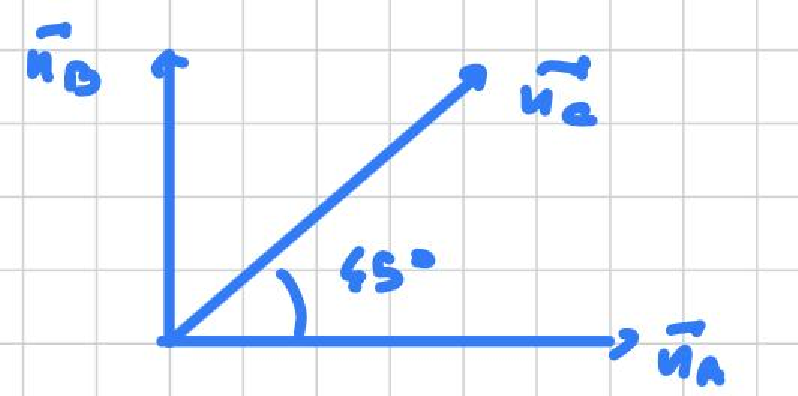
\includegraphics[width=0.6\linewidth]{images_in_pdf/15-/Grafico_82.pdf}
\end{figure}

\[P(\vec{n}_A,\vec{n}_B) =-\vec{n}_A\cdot \vec{n}_B =0 \hspace{1cm} P(\vec{n}_A,\vec{n}_C) = P(\vec{n}_B,\vec{n}_C) = -\frac{\sqrt{2}}{2} = -0.707\]

It can be easily shown that is inconsistent with Bell's inequality:
\[|0-\frac{\sqrt{2}}{2}| \leq 1-\frac{\sqrt{2}}{2} \implies \frac{\sqrt{2}}{2} \cancel{\leq} 1-\frac{\sqrt{2}}{2}\]
if the inequality is not satisfied, Q.M. is correct and hidden variable theory doesn't hold.

\textbf{Experimental test:} suppose to have a structure as 
\begin{figure}[H]
    \centering
    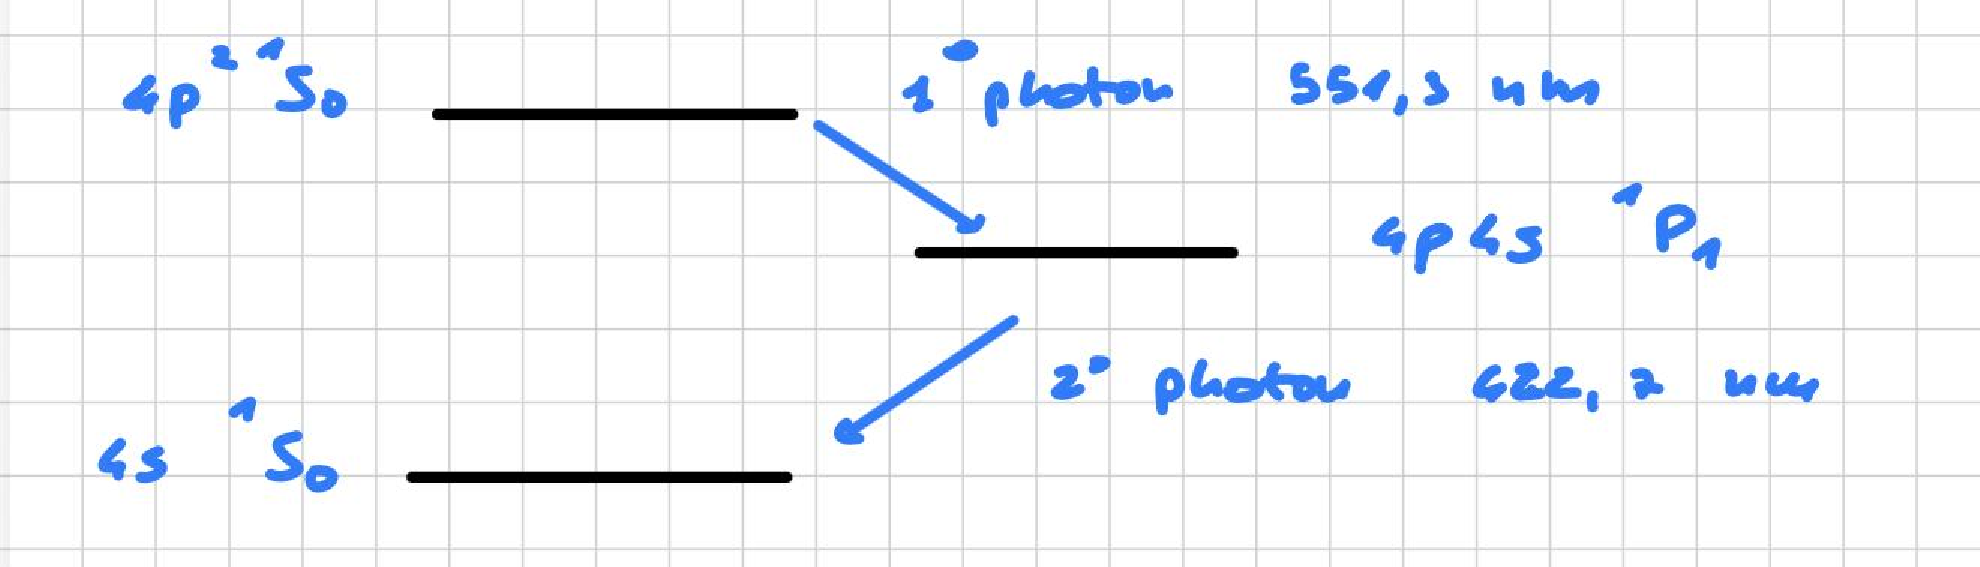
\includegraphics[width=0.6\linewidth]{images_in_pdf/15-/Grafico_83.pdf}
\end{figure}

\begin{itemize}
    \item The ground state and the excited state are $J=0$ states, which means that photon pairs have no net angular momentum.

    \item The parity of the energy levels implies polarization correlation.
\end{itemize}

The set up consists in a beam of $Ca$ atoms which is excite, this generates a pair of photons propagating in opposite directions, each one goes to a PM polarimeter (that measure the linear polarization), a filter $F_i$ (to select photon wavelengths) and then a PMT photomultiplier. Both the photomultipliers are connected to a same electronic system.
\begin{figure}[H]
    \centering
    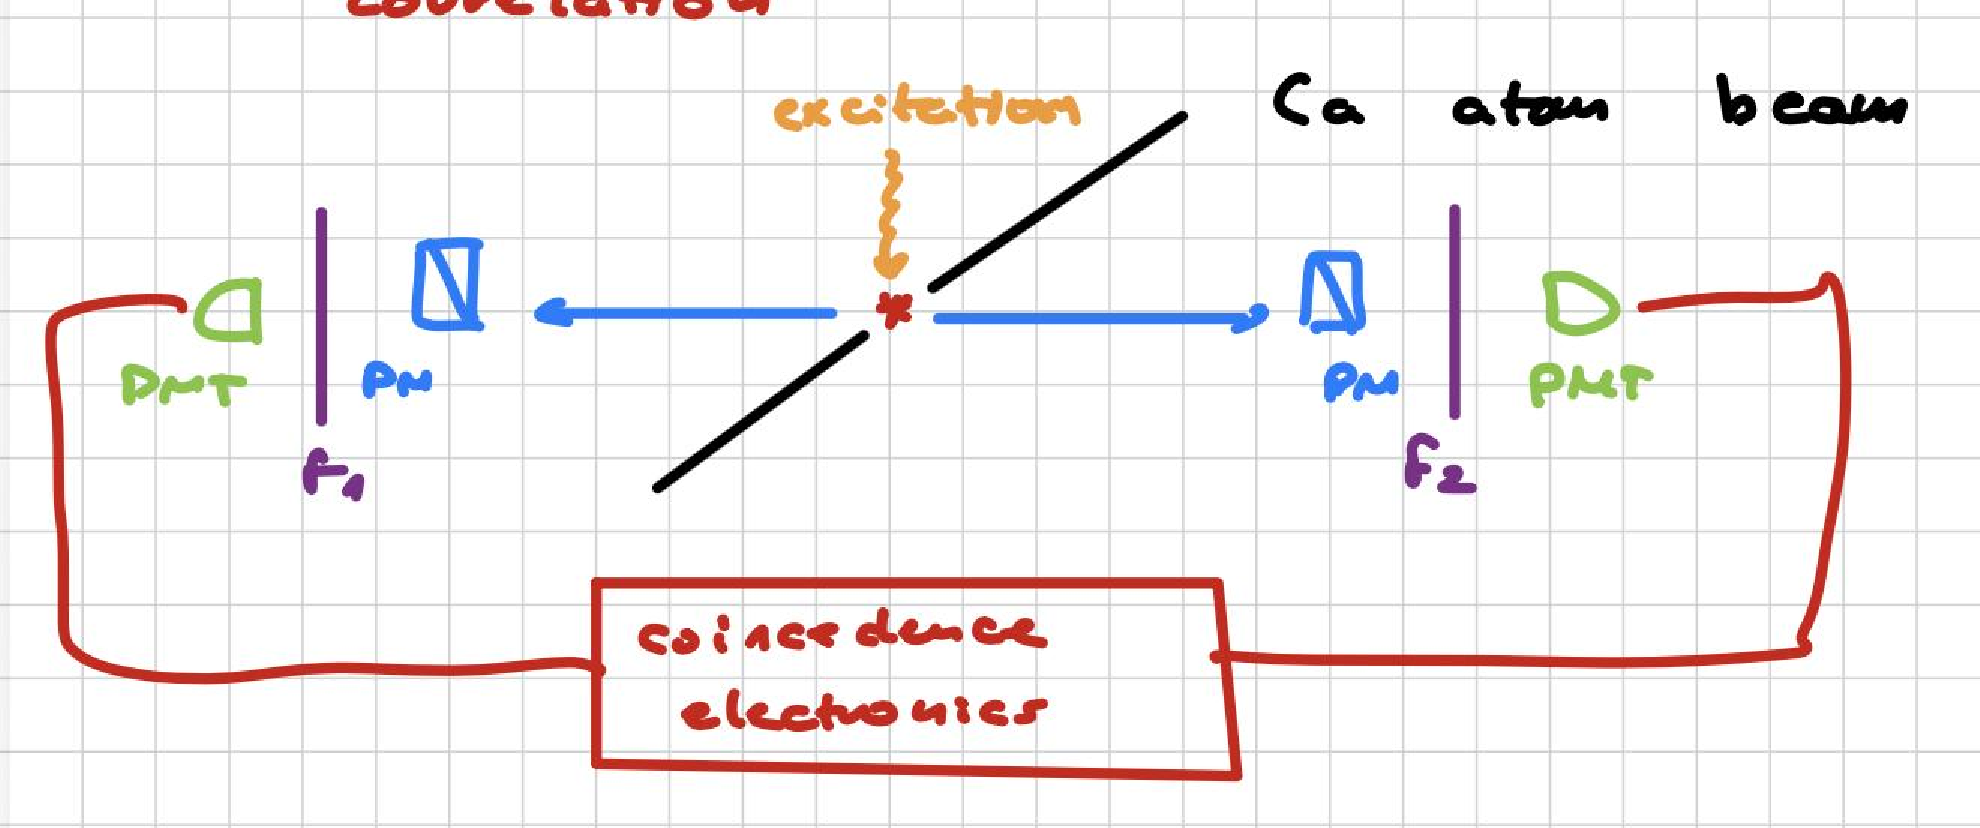
\includegraphics[width=0.6\linewidth]{images_in_pdf/15-/Grafico_84.pdf}
\end{figure}

if we measure along $\vec{n}_A$ direction, this yields to $\ket{V}$ if the polarization is parallel to $\vec{n}_A$ or $\ket{H}$ if the polarization is perpendiculare to $\vec{n}_A$. We can define the \textbf{correlation coefficient:}
\[E(\vec{n}_A,\vec{n}_B) = P_{VV}(\vec{n}_A,\vec{n}_B)+P_{HH}(\vec{n}_A,\vec{n}_B)-P_{VH}(\vec{n}_A,\vec{n}_B)-P_{HV}(\vec{n}_A,\vec{n}_B)\]

Let us consider a combination for two different orientations $(\vec{n}_A,\vec{n}_A')$ and $(\vec{n}_B,\vec{n}_B')$ of the polarizers:
\[S = E(\vec{n}_A,\vec{n}_B)-E(\vec{n}_A',\vec{n}_B')+ E(\vec{n}_A,\vec{n}_B')+E(\vec{n}_A',\vec{n}_B)\]

In realistic local theory view the Bell inequality reads:
\[-2\leq S\leq 2\]
Instead according to Q.M. for particular orientations of $(\vec{n}_A,\vec{n}_A')$ and $(\vec{n}_B,\vec{n}_B')$, we can obtain:
\[S = \pm 2\sqrt{2}\]
this result contradicts the Bell inequality called \textbf{CSCH inequality}.

If we choose a orientation such that:
\[\vec{n}_A\cdot\vec{n}_B = \vec{n}_A'\cdot\vec{n}_B = \vec{n}_A'\cdot\vec{n}_B' = \cos(\theta) \hspace{1cm} \vec{n}_A\cdot\vec{n}_B' = cos(3\theta)\]

We obtain:
\[S = 3\cdot \cos(2\theta)-\cos(6\theta)\]

it is possible to see that for $0\leq \theta \leq 90$ there are some values of S that violate the Bell's inequality, this show us the M.Q. prediction with:
\[S = 2.697\pm 0.015 \hspace{1cm} \theta = \qty{22.5}{\degree}\]

\begin{figure}[H]
    \centering
    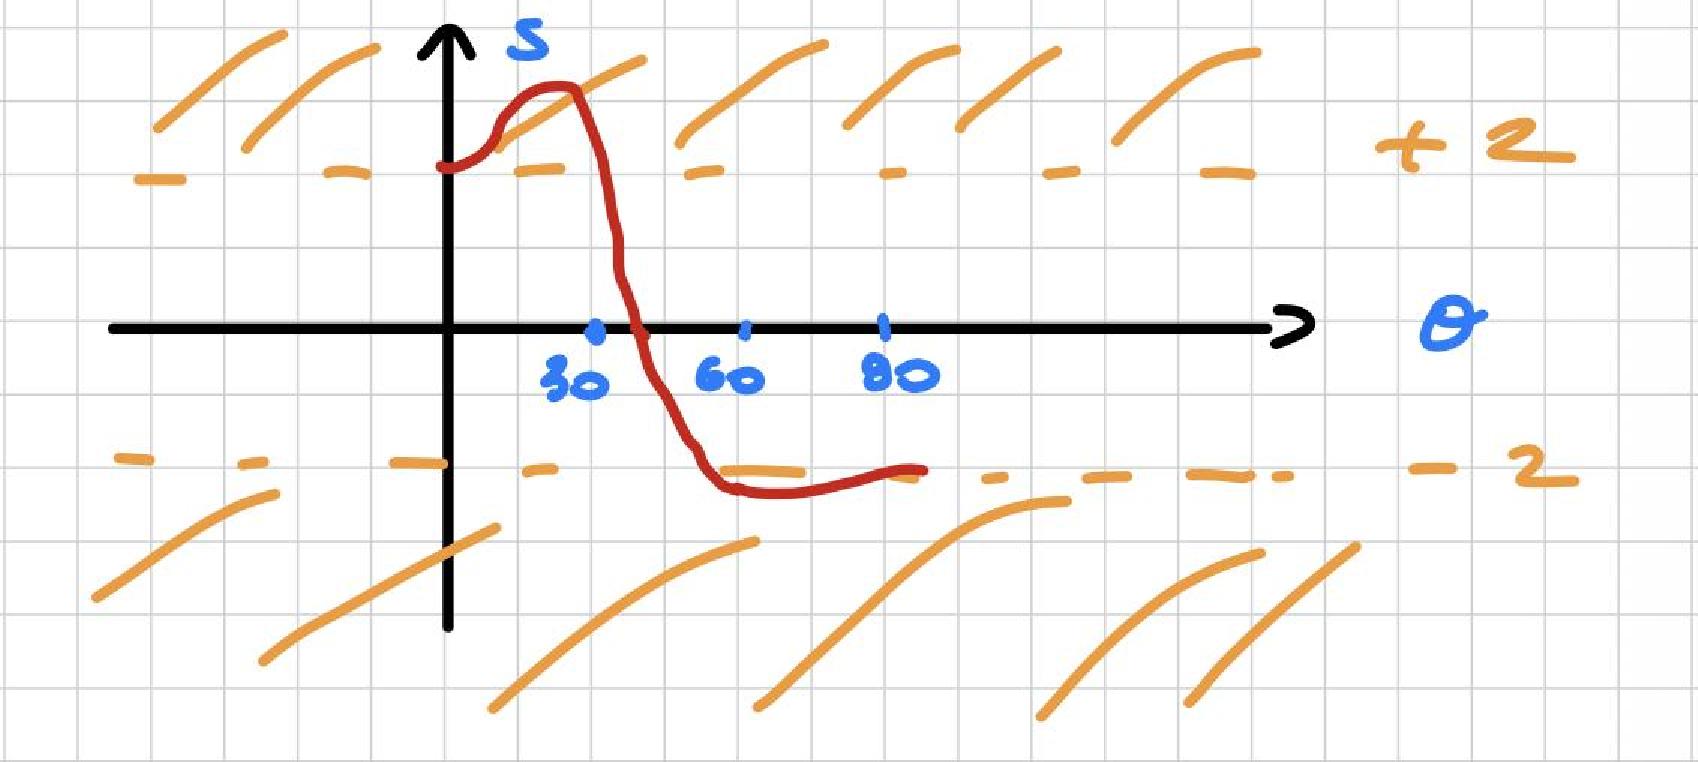
\includegraphics[width=0.6\linewidth]{images_in_pdf/15-/Grafico_85.pdf}
\end{figure}

One must also consider the \textbf{loop-hole problem}. In principle, there is always a possibility that the two measurement stations exchange information during the experiment. To suppress this possibility, the setup can be improved by adding two more photomultipliers and two acousto-optic devices, which change the refractive index of the crystal through sound waves driven by a transducer. The switching time is about $20\,\mathrm{ns}$, which is much smaller than the light travel time between the two stations, $\Delta t \ll L/c$, where $L$ is the distance between the polarizers.

Other possible loopholes are:
\begin{itemize}
    \item \textbf{Freedom-of-choice loophole:} the orientation settings of the analyzers must be chosen independently of the properties of the particle pair.
    
    \item \textbf{Detection loophole:} only a subset of the emitted pairs is detected, so one could argue that the recorded events are not representative of the whole ensemble. This loophole is closed only when the detection efficiency is sufficiently high, typically around $\eta \approx 83\%$ in the standard CHSH scenario.
\end{itemize}

A fully loophole-free experimental demonstration was achieved in 2015 using advanced quantum technologies.

Bell's result does not show that faster-than-light signals exist, but rather that no theory based on \textbf{local hidden variables} can reproduce all the quantum predictions. In a local hidden-variable model, each photon in an entangled pair is assumed to carry predetermined local properties before the measurement is performed. Bell derived an inequality that any such theory must satisfy, and experiments have repeatedly violated this inequality. 
This means that the state of the system is not fully encoded in pre-existing local properties before the measurement.
}

% / / / / / / / / / / / / / / / / / / / / / / / / / / / / / / / / / / / / / / / /
% / / / / / / / / / / / / / / / / / / / / / / / / / / / / / / / / / / / / / / / /

\subsection{Bell experiment}

The core of John Bell's theorem relies on a setup where the orientation of two distant polarizers can be adjusted completely independently. Let polarizer A be oriented along the direction $\vec{n}_A$ and polarizer B along $\vec{n}_B$. Bell proposed to evaluate the statistical correlation between the two measurement stations by computing the expectation value (average) of the product of the polarization outcomes for a given pair of entangled photons.

According to quantum mechanics, the correlation function for a polarization-entangled singlet-like state is given by:
\begin{equation}\label{eqn:15-quantum-correlation}
P(\vec{n}_A,\vec{n}_B) = -\vec{n}_A\cdot\vec{n}_B.
\end{equation}

Bell demonstrated that this quantum mechanical result is fundamentally incompatible with any local hidden-variable (LHV) theory. By introducing a third alternative polarizer orientation $\vec{n}_C$, one can derive the classic \textbf{Bell inequality}:
\begin{equation}\label{eqn:15-bell-inequality}
|P(\vec{n}_A,\vec{n}_B)-P(\vec{n}_A,\vec{n}_C)| \leq 1 + P(\vec{n}_B,\vec{n}_C),
\end{equation}
which must strictly hold for any LHV model. To prove that quantum mechanics violates this constraint, let us select three specific coplanar polarization directions separated by $45^\circ$, such that:

\begin{figure}[H]
    \centering
    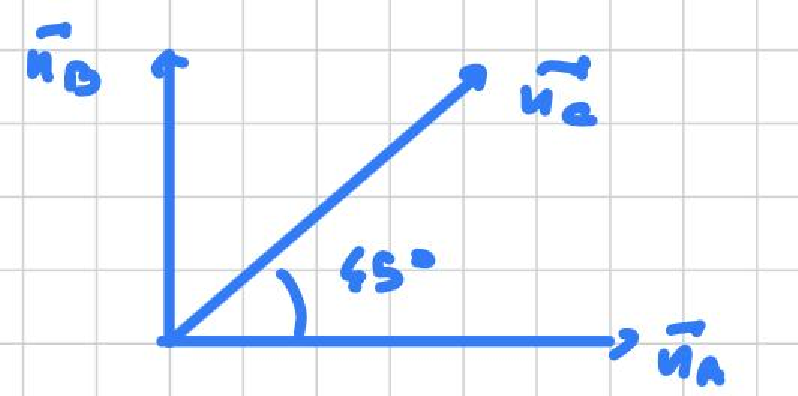
\includegraphics[width=0.6\linewidth]{images_in_pdf/15-/Grafico_82.pdf}
\end{figure}

Evaluating the quantum mechanical correlations yields:
\[
P(\vec{n}_A,\vec{n}_B) =-\vec{n}_A\cdot \vec{n}_B = 0, \qquad P(\vec{n}_A,\vec{n}_C) = P(\vec{n}_B,\vec{n}_C) = -\cos(45^\circ) = -\frac{\sqrt{2}}{2} \approx -0.707.
\]

Substituting these values directly into Bell's inequality leads to an explicit contradiction:
\[
\left|0 - \left(-\frac{\sqrt{2}}{2}\right)\right| \leq 1 + \left(-\frac{\sqrt{2}}{2}\right) \implies \frac{\sqrt{2}}{2} \not\leq 1 - \frac{\sqrt{2}}{2},
\]
since $0.707 \not\leq 0.293$. This geometric violation formally proves that quantum mechanics cannot be reproduced by any local deterministic hidden-variable framework.

\callout{Uselessy formal discussion of the CHSH inequality violation}{%

Suppose Alice and Bob are two observers who can independently choose between two measurement settings, denoted as $a$ and $a'$ for Alice, and $b$ and $b'$ for Bob. All these measurements have the same possible outcomes: $\pm 1$. Each one of them has access to one out of two correlated particles. 
\begin{equation}\label{eqn:15-chsh-scheme}
\begin{aligned}
&\text{Alice measures}\quad &&\text{Bob measures} \\
&a, a' = \pm 1 && b, b' = \pm 1\\
\end{aligned}
\end{equation}

We can introduce a derived observable $C$ defined as:
\begin{equation}\label{eqn:15-chsh-observable}
    C = (a+a')b + (a-a')b'
\end{equation}

which, by construction, can only take the values $\pm 2$:
\begin{equation}\label{eqn:15-chsh-values}
\begin{cases}
    a   =  a' \implies a+a' = \pm2,\ a-a'=0\\
    a \neq a' \implies a+a' = 0,\ a-a' = \pm2
\end{cases}
\implies
C = \pm 2,\ \forall\, a, a', b, b'.
\end{equation}

for any observable, it must hold that:
\begin{equation}\label{eqn:15-triangular-inequality}
    |\braket{C}| \leq \braket{|C|} 
\end{equation}

since $|C|=2$, we find the CHSH inequality:
\begin{equation}\label{eqn:15-chsh-inequality}
    |\braket{C}| \leq 2.
\end{equation}

in the photonic picture, the observables $a$ and $a'$ can be seen as polarization measurements in two different basis (e.g. horizontal-vertical or diagonal plus-minus); same applies for $b$ and $b'$. 

We now show that quantum mechanics predicts a violation of the CHSH inequality. 
\begin{proof}

Suppose that the couples of particles shared by Alice and Bob are prepared in a maximally entangled state, such as the singlet state:
\begin{equation}\label{eqn:15-singlet-state}
    \ket{\psi} = \frac{1}{\sqrt{2}} \,  \bigl(\ket{0,1}-\ket{1,0}\bigr).
\end{equation}

where $\ket{0}$ and $\ket{1}$ are eigenvectors of any couple of the observables measurable by Alice and Bob. There's no need to be more specific than this.

\end{proof}
}


\subsubsection{Experimental test} 
To test this prediction in the laboratory, one can exploit an atomic cascade source. Consider a calcium (\ce{Ca}) atom characterized by the following energy-level structure:

\begin{figure}[H]
    \centering
    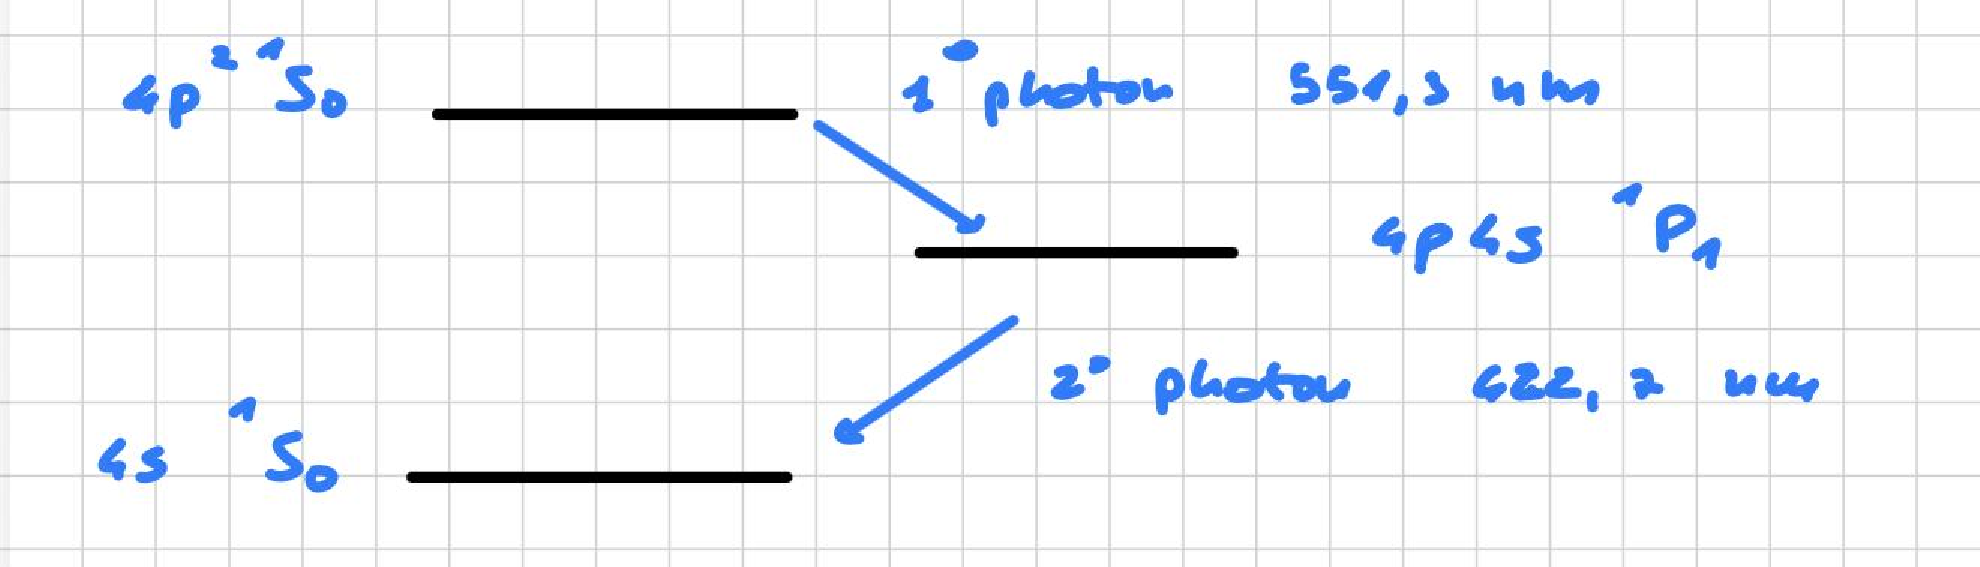
\includegraphics[width=0.6\linewidth]{images_in_pdf/15-/Grafico_83.pdf}
\end{figure}

\begin{itemize}
    \item Both the ground state and the excited state are $J=0$ angular momentum states, meaning the \hl{emitted photon pairs carry no net total angular momentum};
    \item The well-defined parity of these energy levels enforces a strict polarization correlation between the two photons to conserve total angular momentum.
\end{itemize}

The experimental setup consists of a calcium atomic beam excited via a two-photon process. The subsequent cascade decay generates a pair of entangled photons propagating in opposite directions. Each photon is directed toward a measurement arm containing a wavelength filter $F_i$ (to isolate the respective cascade transition), a linear polarimeter to analyze the polarization along $\vec{n}_i$, and a high-sensitivity photomultiplier tube (PMT). Both PMTs are connected to a central coincidence electronics system to register simultaneous detection events.

\begin{figure}[H]
    \centering
    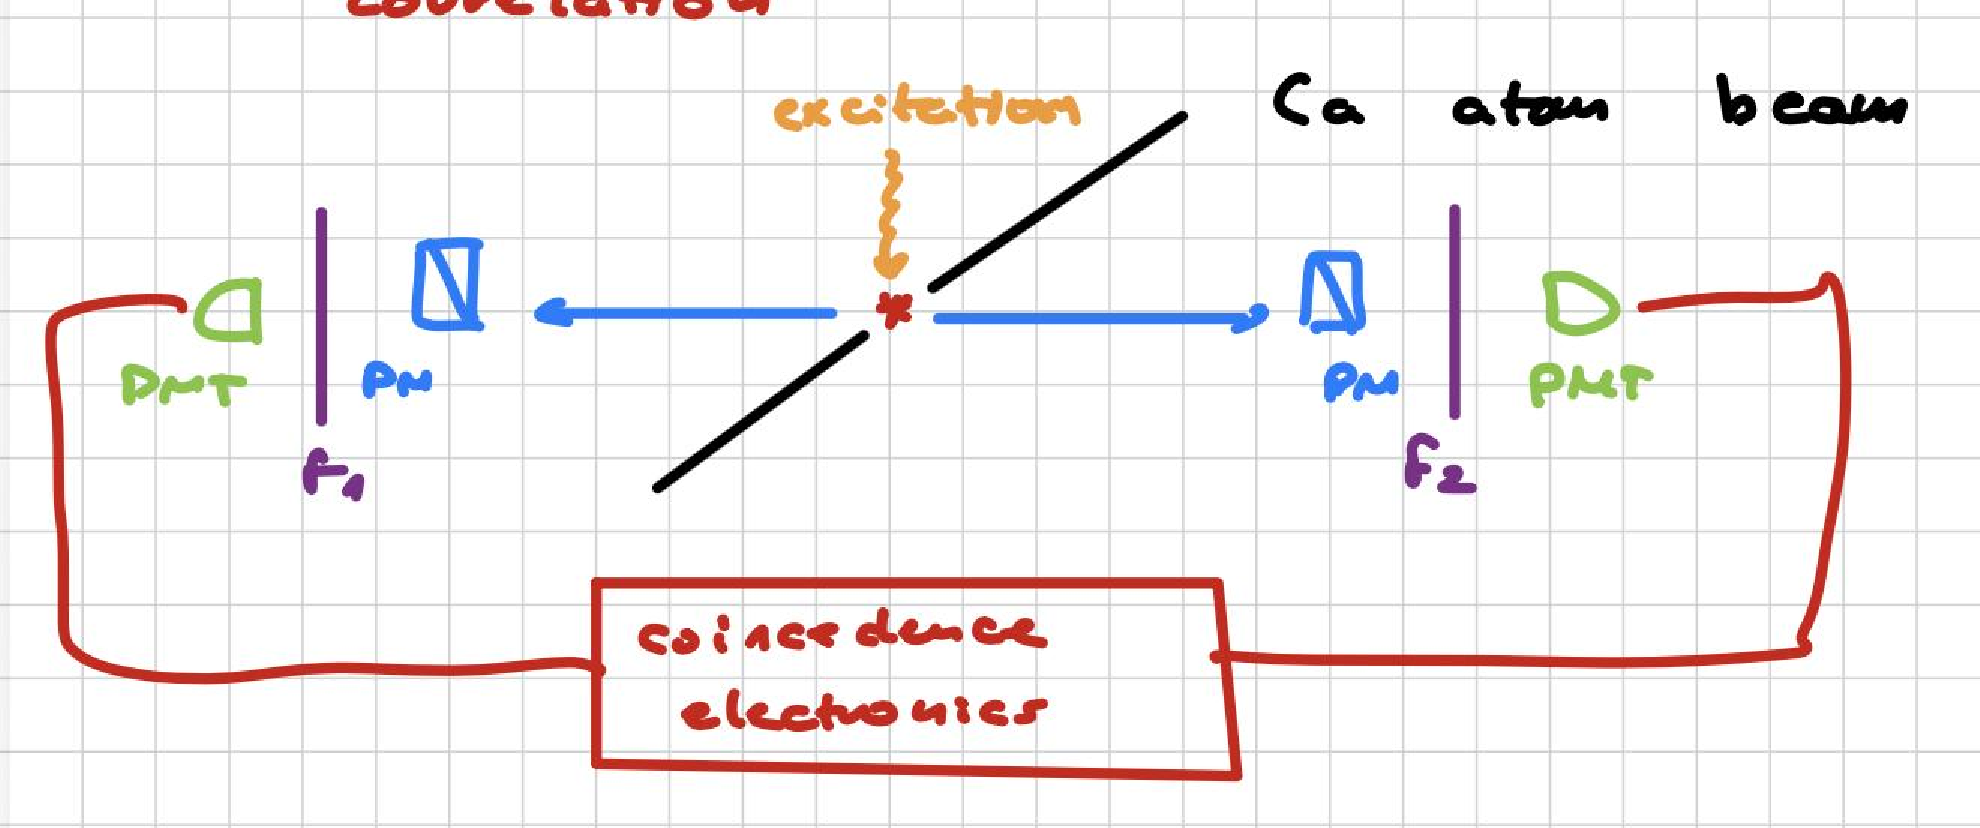
\includegraphics[width=0.6\linewidth]{images_in_pdf/15-/Grafico_84.pdf}
\end{figure}

A measurement along the $\vec{n}_A$ direction yields a vertical outcome $\ket{V}$ if the photon polarization is parallel to $\vec{n}_A$, or a horizontal outcome $\ket{H}$ if it is perpendicular. We can then define the experimental \textbf{correlation coefficient} $E(\vec{n}_A,\vec{n}_B)$ as:
\begin{equation}\label{eqn:15-correlation-coefficient}
E(\vec{n}_A,\vec{n}_B) = P_{VV}(\vec{n}_A,\vec{n}_B) + P_{HH}(\vec{n}_A,\vec{n}_B) - P_{VH}(\vec{n}_A,\vec{n}_B) - P_{HV}(\vec{n}_A,\vec{n}_B),
\end{equation}
where $P_{ij}$ represents the joint probability of detecting outcome $i$ at station A and outcome $j$ at station B.

To maximize the experimental violation, we consider a combination of four distinct polarizer orientations -- $\vec{n}_A, \vec{n}_A'$ for Alice and $\vec{n}_B, \vec{n}_B'$ for Bob -- grouped into the $\mathbf{S}$\textbf{-parameter}:
\begin{equation}\label{eqn:15-s-parameter}
S = E(\vec{n}_A,\vec{n}_B) + E(\vec{n}_A,\vec{n}_B') + E(\vec{n}_A',\vec{n}_B) - E(\vec{n}_A',\vec{n}_B').
\end{equation}

\hl{In any realistic local theory, this expression is bounded by the \textbf{CHSH inequality}} (Clauser-Horne-Shimony-Holt):
\begin{equation}\label{eqn:15-chsh-bounds}
-2 \leq S \leq 2.
\end{equation}

Conversely, quantum mechanics predicts that for polarization-entangled states, the correlation coefficient scales as 
\begin{equation}\label{eqn:15-quantum-correlation-2}
E(\phi) = \cos(2\phi), 
\end{equation}

where $\phi$ is the relative angle between the polarizers. If we choose a geometric configuration where the angular separations are $\theta_{AB} = \theta_{AB'} = \theta_{A'B} = \theta$, while the fourth pair is widely separated by $\theta_{A'B'} = 3\theta$, the $S$-parameter becomes a function of a single angle:
\begin{equation}\label{eqn:15-s-theta}
S(\theta) = 3\cos(2\theta) - \cos(6\theta).
\end{equation}

Maximizing this function at $\theta = \qty{22.5}{\degree}$ yields the maximum quantum mechanical violation known as the Cirel'son bound:
\begin{equation}\label{eqn:15-tsirelson-bound}
S = \pm 2\sqrt{2} \approx \pm 2.828,
\end{equation}
which \hl{heavily contradicts the local realistic limit of $2$}. Historical experiments (such as those by Alain Aspect) closely matched the quantum mechanical predictions, yielding an experimental value of:
\begin{equation}\label{eqn:15-experimental-s-chsh}
S_{\text{exp}} = 2.697 \pm 0.015 \qquad \text{at } \theta = \qty{22.5}{\degree},
\end{equation}

which \hl{rules out local hidden variables by many standard deviations}.

\begin{figure}[H]
    \centering
    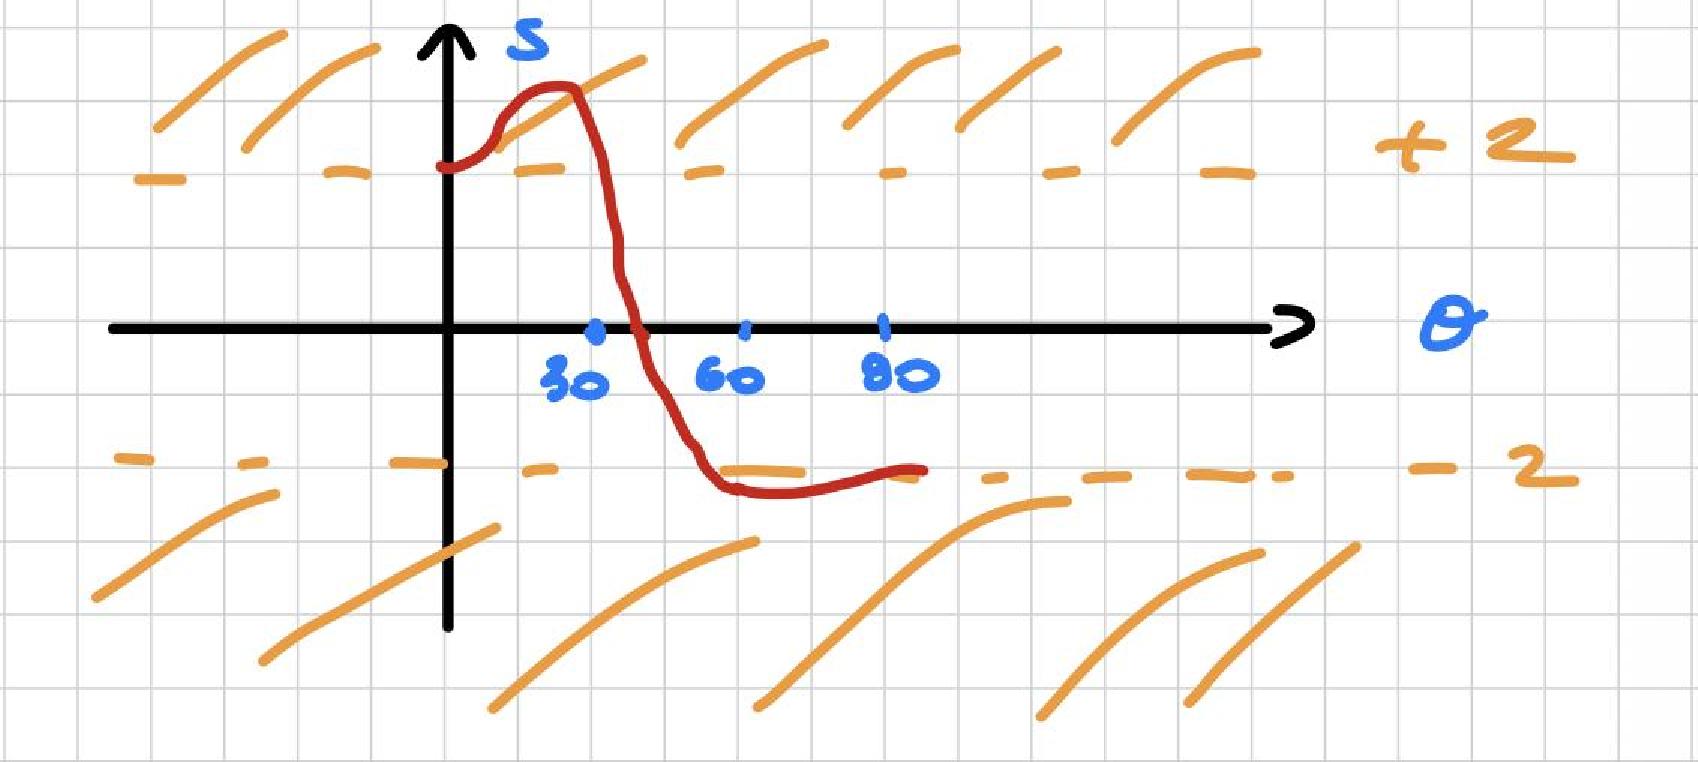
\includegraphics[width=0.6\linewidth]{images_in_pdf/15-/Grafico_85.pdf}
\end{figure}


\subsubsection{Loophole problems}
To ensure the validity of these experimental conclusions, one must address various \hl{experimental vulnerabilities, known as loopholes}, that could potentially allow for local hidden-variable explanations. The main loopholes are:

\begin{itemize}
    \item \textbf{Locality loophole:} There is a risk that the two measurement stations could exchange sub-luminal coordination signals during the photon flight time. To close this loophole, the setup can be upgraded by implementing high-speed acousto-optic modulators (AOMs). Driven by acoustic transducers, these devices switch the optical path between alternative polarizers on a timescale of $\sim \qty{20}{\nano\second}$. Since this switching time is much shorter than the light propagation time between the stations ($\Delta t \ll L/c$, where $L$ is the physical separation), the measurement settings are chosen at space-like separated intervals, preventing any causal communication.
    
    \item \textbf{Freedom-of-choice loophole:} This requires that the random generation of the analyzer settings must be completely independent of any properties or shared history of the entangled particle pair.
    
    \item \textbf{Detection loophole:} If the detectors sample only a small subset of the emitted pairs due to low quantum efficiency $\eta$, one could argue that the recorded events are biased and unrepresentative of the entire ensemble. Closing this loophole requires high-efficiency detectors; in a standard CHSH scenario, the symmetric detection efficiency threshold must satisfy $\eta \gtrsim 83\%$.
\end{itemize}

A fully loophole-free experimental demonstration -- simultaneously closing the locality, freedom-of-choice, and detection loopholes -- was successfully achieved in 2015. 

\calloutinfo{%
    Ultimately, Bell's theorem does not imply the existence of faster-than-light signaling, but rather demonstrates that \textbf{no local realistic theory can reproduce the non-local correlations of quantum mechanics}. Entangled photons do not carry predetermined local properties before a measurement is performed; their physical state is not fully encoded in pre-existing local variables, but is established contextually at the moment of detection.
}

\section{Optical tests of Quantum Mechanics}\label{sec:optical-tests-qm}

We have a pump beam photon at frequency $\omega_p$ (high energy $\approx$ UV-visible) which excites a non-linear crystal and is converted into two photons (visible-IR), one in the \textbf{signal} $\omega_s$ and one into the \textbf{idler} beam $\omega_i$. 
\begin{figure}[H]
    \centering
    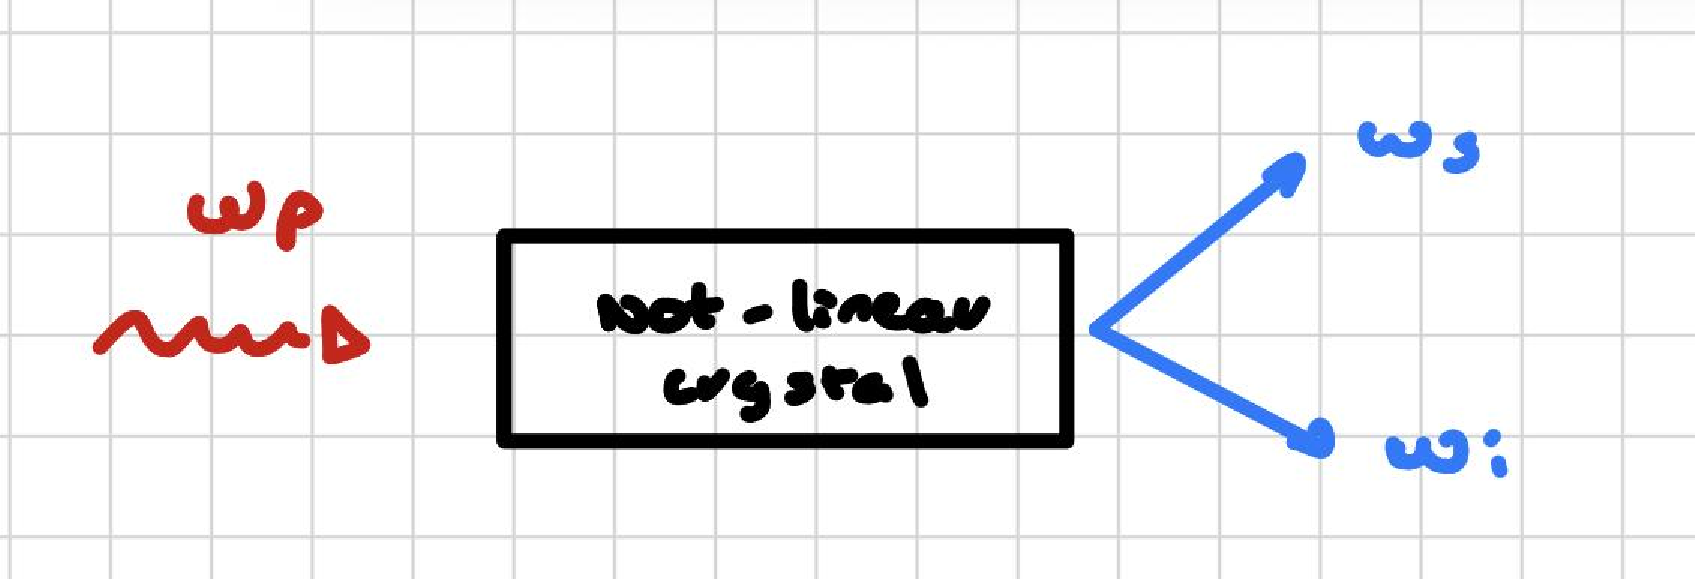
\includegraphics[width=0.6\linewidth]{images_in_pdf/16-/Grafico_86.pdf}
\end{figure}

We assume that the \hl{pump field is quantized} and the interaction Hamiltonian have the form:
\begin{equation}\label{eqn:16-interaction-hamiltonian}
\hat{H} \propto \chi^{(2)}\, \hat{a}_p\, \hat{a}_s^+\, \hat{a}_i^+ 
\end{equation}

Where \hl{$\chi^{(2)}$ is the second order non-linear susceptibility} and it cames from the polarization when we consider non-centrosymmetric crystals:
\begin{equation}\label{eqn:16-polarization-non-linear}
\vec{P} = \epsilon_0 \, \chi \, \vec{E}+ \epsilon_0 \, \chi^{(2)}\, \vec{E}^2+...
\end{equation}

\hl{$\hat{a}_p$ is the annihilation operator of the pump beam, $\hat{a}_s^+$ is the creation operator for the signal and $\hat{a}_i^+$ is the creation operator for the idler wave}.

Initially we have a sigle photon state for the pump, joint with a vacuum state for signal and idler, then we obtain through a \textbf{spontaneous process:}
\begin{equation}\label{eqn:16-spontaneous-process}
\hat{a}_p\, \hat{a}_s^+\, \hat{a}_i^+ \, \ket{1}_p\ket{0}_s\ket{0}_i = \ket{0}_p\ket{1}_s\ket{1}_i
\end{equation}

In order to obtain it we we need to satisfy some requirements called \textbf{Phase matching conditions}:
\begin{itemize}
    \item \emph{Conservation of energy}:
    \begin{equation}\label{eqn:16-phase-matching-energy}
    \hbar \omega_p = \hbar\omega_s+\hbar\omega_i
    \end{equation}

    \item \emph{Conservation of momentum}:
    \begin{equation}\label{eqn:16-phase-matching-momentum}
    \hbar \vec{k}_p =\hbar \vec{k}_s+\hbar \vec{k}_i
    \end{equation}
\end{itemize}

Typically we use a UV photon and obtain two IR photons, notice that to satisfy them also the direction of the beam is important.

\calloutinfo{%
    In the so called \textbf{Type II} crystals the polarizations of signal and idler photons are orthogonal, this makes it possible to generate \textbf{entangled states}:
\begin{equation}\label{eqn:16-entangled-state}
\ket{\psi} = \frac{1}{\sqrt{2}}\, 
\bigl[ 
    \ket{H}_s\ket{V}_i+\ket{V}_s\ket{H}_i
\bigr]
\end{equation}

In case instead of a \textbf{Type I} crystal, the polarizations of signal and idler are the same: we don't obtain entangled photons, but it can be useful in order to have a indistinguishable photon source.
}

\subsection{Interference experiments}
We are interested in understanding what happens if our twin single photons are simultaneously incident at each input port of a B.S.

We need to describe the B.S. with quantum mechanics: 
\begin{figure}[H]
    \centering
    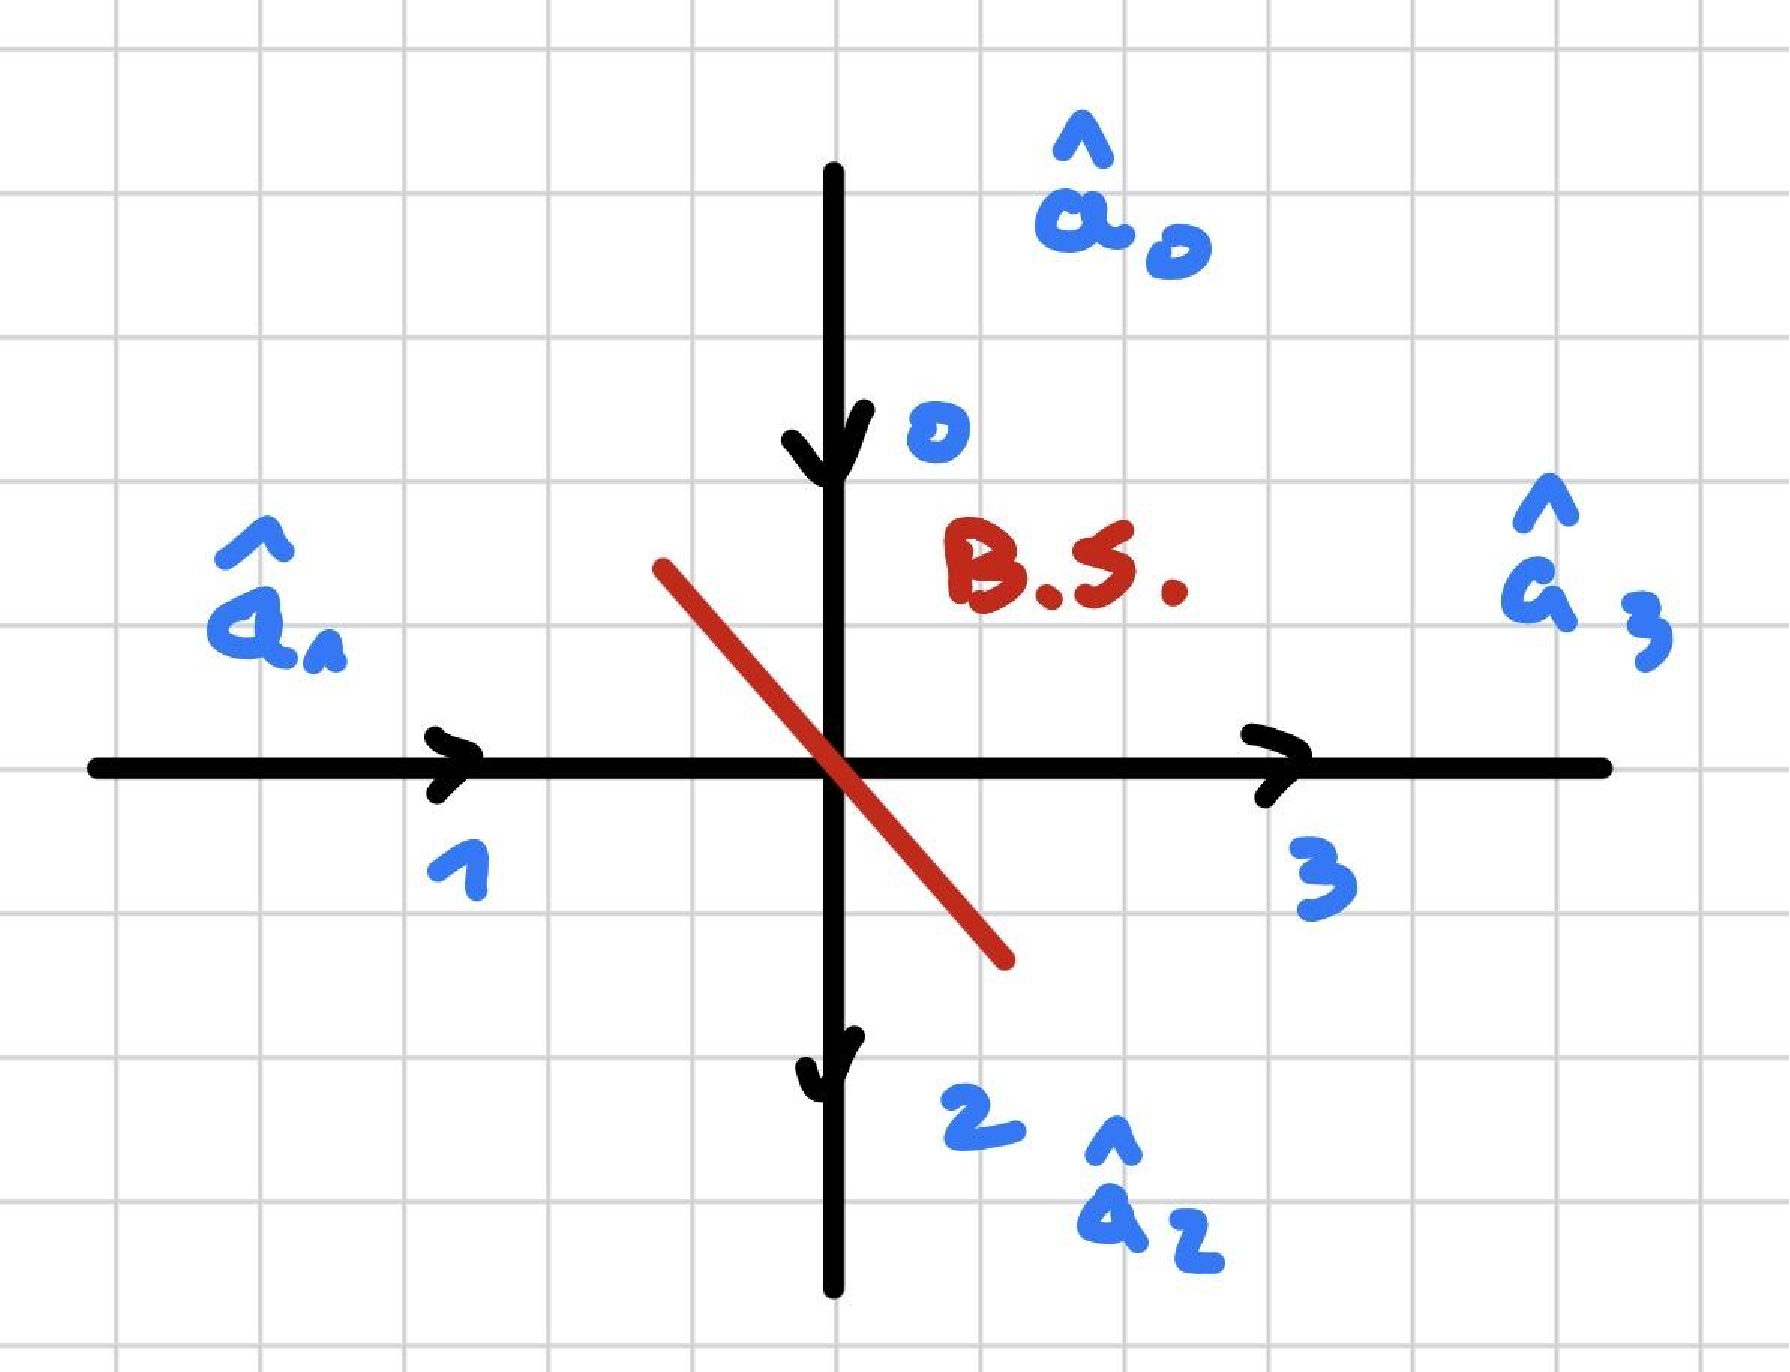
\includegraphics[width=0.6\linewidth]{images_in_pdf/16-/Grafico_87.pdf}
\end{figure}

Let's consider a B.S. with two input ports $1$ and $0$ and two exit ports $2$ and $3$, for each we can associate an annihilation operator $\hat{a}_i$.

If $\refl$ and $\tran$ are the complex \textbf{reflectance} and \textbf{transmittance} of the beam splitter B.S., \hl{from the classical point of view we send an electric field $E_1$ which is transmitted as $E_3$ and reflected as $E_2$}:
\begin{equation}\label{eqn:16-classical-b-s}
\begin{cases}
    E_2 = \refl\, E_1\\[0.5ex]
    E_3 = \tran\, E_1
\end{cases}
\end{equation}

Where $E_i$ stands for the complex amplitude of the light field; for a $50:50$ B.S. we will obtain:
\begin{equation}\label{eqn:16-50-50-b-s}
\begin{cases}
    |\refl| = |\tran| = \frac{1}{\sqrt{2}}\\[0.5ex]
    |\refl|^2 + |\tran|^2 =1
\end{cases}
\end{equation}

\hl{According to quantum mechanics, we must consider the equivalent coefficients $\refl,\tran \to \refl',\tran'$ for the input port $0$ which correspond to a vacuum state}:
\begin{equation}\label{eqn:16-quantum-b-s}
\begin{cases}
    \hat{a}_2 = \refl\,\hat{a}_1+\tran'\,\hat{a}_0\\[0.5ex]
    \hat{a}_3 = \tran\, \hat{a}_1+\refl'\, \hat{a}_0
\end{cases}\implies \begin{pmatrix}
    \hat{a}_2\\[0.5ex]
    \hat{a}_3
\end{pmatrix} = \begin{pmatrix}
    \refl' &\tran\\[0.5ex]
    \tran' &\refl
\end{pmatrix}\begin{pmatrix}
    \hat{a}_0\\[0.5ex]
    \hat{a}_1
    \end{pmatrix}
\end{equation}

For a $50:50$ B.S. reflected and transmitted beams have the same amplitude, but they are different in phase:
\begin{equation}\label{eqn:16-50-50-b-s-phase}
\begin{cases}
    \hat{a}_2= \frac{1}{\sqrt{2}}\, 
    \left( \hat{a}_0+i\hat{a}_1\right)\\[0.5ex]
    \hat{a}_3= \frac{1}{\sqrt{2}}\, 
    \left( i\hat{a}_0+\hat{a}_1\right)
\end{cases}
\end{equation}

\subsubsection{One photon and vacuum state at the input ports}

Let's discuss the case where we have a single photon arriving at the input port $1$, so that the two initial states can be rewritten as functions of the creation operators:
\begin{equation}\label{eqn:16-single-photon-state}
\ket{0}_0\ket{1}_1 = \hat{a}_1^\dagger \, \ket{0}_0\ket{0}_1
\end{equation}

From previous equations and taking the dagger, we can rewrite:
\begin{equation}\label{eqn:16-b-s-creation-operators}
\begin{split}
\hat{a}_3^\dagger +i\hat{a}_2^\dagger  &= \frac{1}{\sqrt{2}}
\bigl[
    -i\hat{a}_0^\dagger +\hat{a}_1^\dagger +i(\hat{a}_0^\dagger -i\hat{a}_1^\dagger )
\bigr] = \\[0.5ex]
&= \frac{1}{\sqrt{2}}
\bigl[
    \cancel{-i\hat{a}_0^\dagger }+\hat{a}_1^\dagger +\cancel{i\hat{a}_o^+}+\hat{a}_1^\dagger 
\bigr] = \\[0.5ex]
&= \frac{1}{\sqrt{2}} \, 2\hat{a}_1^\dagger \\[0.5ex]
\iff \hat{a}_1^\dagger  &= \frac{1}{\sqrt{2}}(\hat{a}_3^\dagger +i\hat{a}_2) 
\end{split}
\end{equation}

Notice also that the action of B.S. on vacuum state entering input port gives as result: 
\begin{equation}\label{eqn:16-vacuum-state}
\ket{0}_0\ket{0}_1 \mapsto \ket{0}_2\ket{0}_3
\end{equation}

So we can substitute and obtain:
\begin{equation}\label{eqn:16-single-photon-state-2}
\ket{0}_0\ket{1}_1 = \frac{1}{\sqrt{2}} (i\hat{a}_2^\dagger +\hat{a}_3^\dagger ) \, \ket{0}_2\ket{0}_3 = 
\frac{1}{\sqrt{2}}\, 
\left(
    i\ket{1}_2\ket{0}_3+ \ket{0}_2\ket{1}_3
\right)
\end{equation}

\calloutinfo{%
    We obtained an \textbf{entangled state} between output ports $2$ and $3$, we cannot have coincidence counts! We can have 1 photon only in one arm and never  simultaneously in both.
} 
When we measure one of the two arms we collapse the wave function and destroy the interference.

\subsubsection{Two photons at the input ports}

Let's come back and study the case of twin single photons injected into two ports of the B.S.:

\begin{figure}[H]
    \centering
    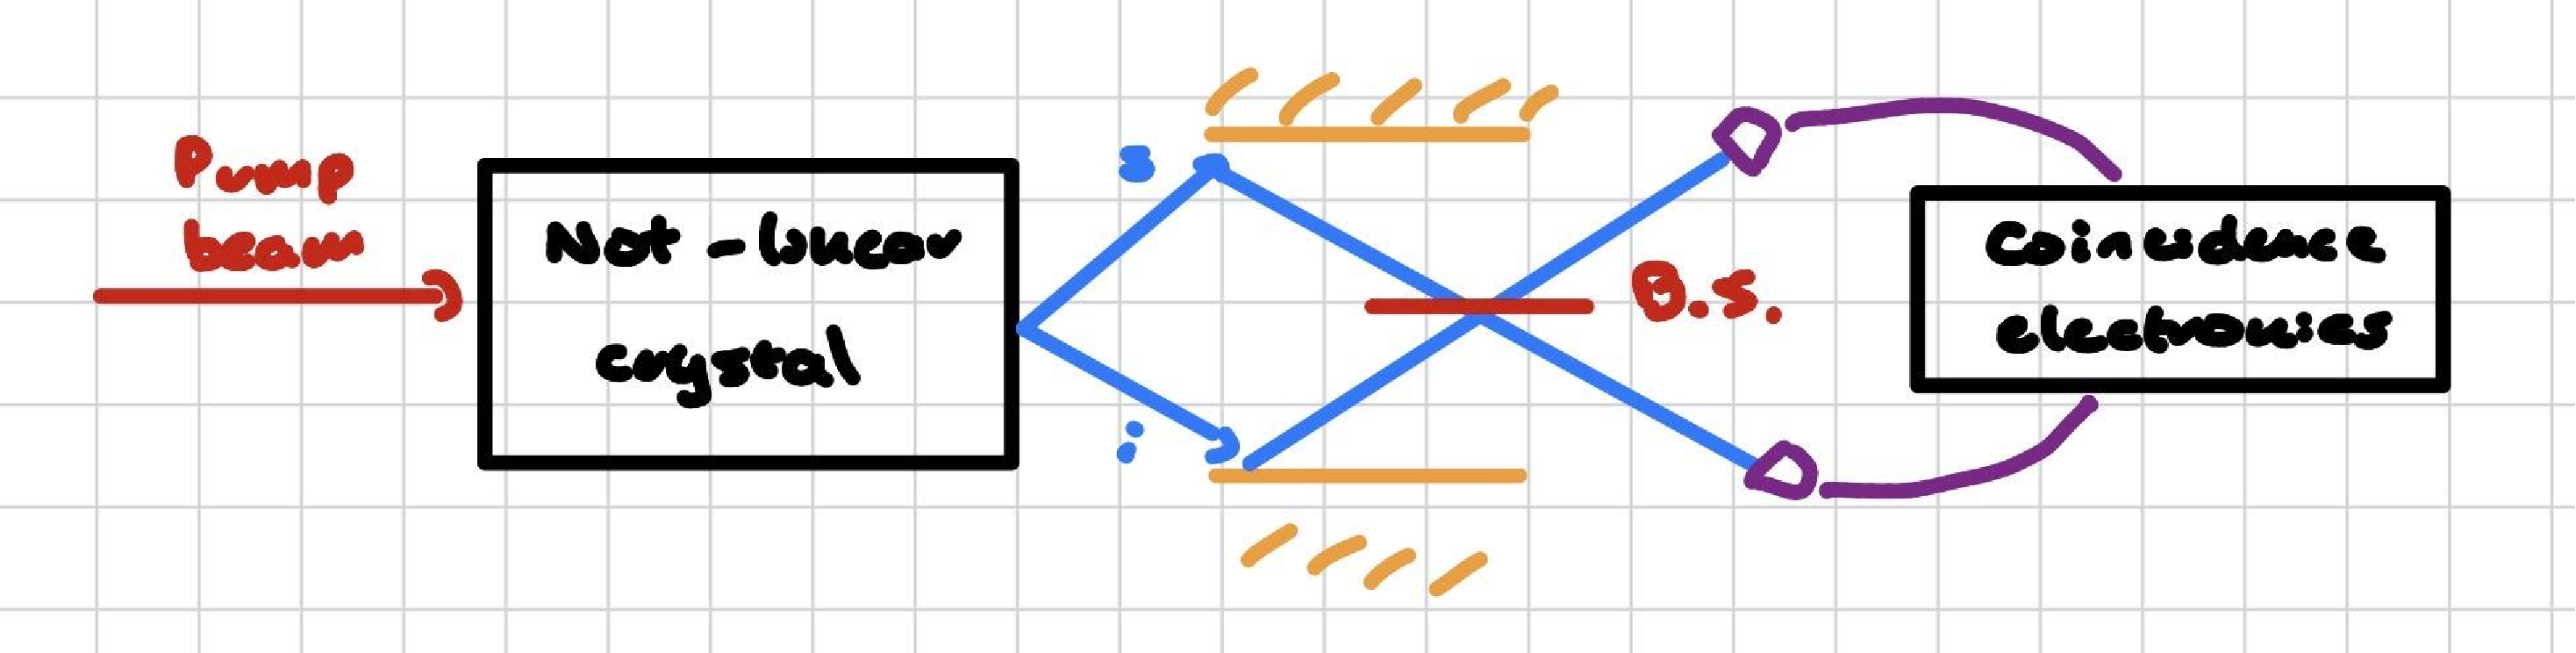
\includegraphics[width=0.6\linewidth]{images_in_pdf/16-/Grafico_88.pdf}
\end{figure}
\begin{figure}[H]
    \centering
    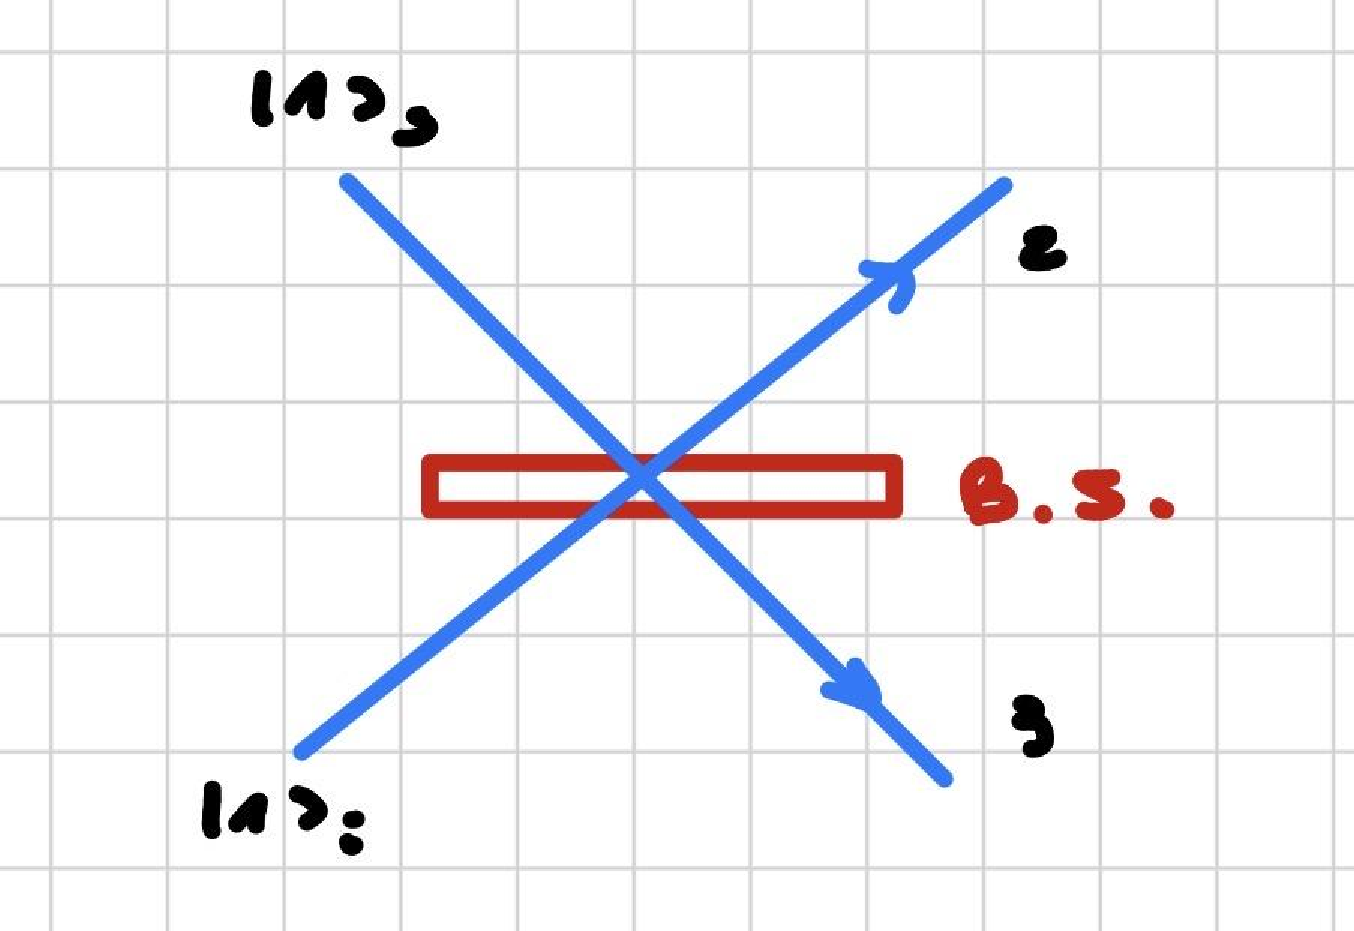
\includegraphics[width=0.6\linewidth]{images_in_pdf/16-/Grafico_89.pdf}
\end{figure}

The pump beam excites a nonlinear crystal, which emits pairs of photons, usually referred to as \textbf{signal} ($s$) and \textbf{idler} ($i$). After removing the pump, the two photons are reflected by mirrors and sent to the two input ports of a balanced beam splitter (BS). The output fields are then collected by two detectors connected to a coincidence circuit in order to perform the measurement.

We send the states $\ket{1}_s$ and $\ket{1}_i$ into the BS. 

\textbf{What should we expect at the output ports?}

As in the previous case, we can rewrite the initial state as
\begin{equation}\label{eqn:16-twin-single-photon-state}
\ket{1}_0\ket{1}_1 = \hat a_0^\dagger \hat a_1^\dagger \ket{0}_0\ket{0}_1,
\end{equation}

where the beam splitter transformation for the creation operators is
\begin{equation}\label{eqn:16-b-s-creation-operators-2}
\begin{cases}
\hat a_0^\dagger = \frac{1}{\sqrt{2}}\left(\hat a_2^\dagger + i\hat a_3^\dagger\right),\\[1ex]
\hat a_1^\dagger = \frac{1}{\sqrt{2}}\left(i\hat a_2^\dagger + \hat a_3^\dagger\right).
\end{cases}
\end{equation}

Moreover, the vacuum is mapped as
\begin{equation}\label{eqn:16-vacuum-state-mapping}
\ket{0}_0\ket{0}_1 \to \ket{0}_2\ket{0}_3.
\end{equation}

Therefore,
\begin{equation}\label{eqn:16-single-photon-state-3}
\begin{split}
    \implies \ket{1}_0\ket{1}_1 &= 
    \frac{1}{\sqrt{2}}\frac{1}{\sqrt{2}}
    \left(\hat{a}_2^\dagger +i\hat{a}_3^\dagger \right)\, 
    \left(i\hat{a}_2^\dagger +\hat{a}_3^\dagger \right)\, 
    \ket{0}_2\ket{0}_3 = \\[0.5ex]
    &=\frac{i}{2}
    \left(\hat{a}_2^\dagger \hat{a}_2^\dagger +\hat{a}_3^\dagger \hat{a}_3^\dagger \right) \ket{0}_2\ket{0}_3 \propto \\[0.5ex]
    &\propto i\,
    \bigl(\ket{2}_2\ket{0}_3+\ket{0}_2\ket{2}_3\bigr) 
    = \ket{\psi}_{B.S.}
\end{split}
\end{equation}

The disappearance of the central terms in the expansion is a direct consequence of both the bosonic nature of photons and the phase relations introduced by the beam splitter. The mixed terms $\hat a_2^\dagger \hat a_3^\dagger$ and $\hat a_3^\dagger \hat a_2^\dagger$ correspond to the configuration in which one photon exits each output port, i.e. the state $\ket{1}_2\ket{1}_3$. Since photons are bosons, operators acting on different ports commute, $\hat a_2^\dagger \hat a_3^\dagger = \hat a_3^\dagger \hat a_2^\dagger$, and these two contributions cancel exactly due to their opposite relative phase. As a result, \hl{the coincidence term vanishes}.

\hl{This implies that both photons always leave the beam splitter through the same output port}. This behavior cannot be understood within a classical picture based on independent trajectories, but arises from quantum interference between indistinguishable processes. 
In particular, there are two possible ways to obtain a coincidence event: 
\begin{enumerate}
\item Both photons being transmitted;
\item Both photons being reflected.
\end{enumerate}

\hl{Since these processes are indistinguishable, their probability amplitudes must be summed before taking the modulus squared}, leading to \textbf{destructive interference} and a vanishing coincidence probability.

Defining the transmission and reflection amplitudes as
\begin{equation}\label{eqn:16-b-s-amplitudes}
A_\tran = \frac{1}{\sqrt{2}}, \qquad A_\refl = \frac{i}{\sqrt{2}},
\end{equation}

the coincidence amplitude is
\begin{equation}\label{eqn:16-coincidence-amplitude}
A_\tran A_\tran + A_\refl A_\refl = \frac{1}{2} + \frac{i^2}{2} = 0,
\end{equation}

and therefore
\begin{equation}\label{eqn:16-coincidence-probability}
P_{11} = \left|A_\tran A_\tran + A_\refl A_\refl\right|^2 = \left|\frac{1}{\sqrt{2}}\frac{1}{\sqrt{2}}+\frac{i}{\sqrt{2}}\frac{i}{\sqrt{2}}\right|^2 = 0
\end{equation}

\calloutinfo{%
    In the ideal case, coincidences are completely suppressed, and the output state is a two-photon bunched state.
    This effect cannot be interpreted classically; it is a direct consequence of two-photon interference and bosonic symmetry.
}

\subsubsection{Hong-Ou-Mandel proof-of-principle experiment}

In 1982, Hong, Ou, and Mandel demonstrated two-photon interference using a \textbf{type-I nonlinear crystal} with the setup shown below. The pump beam excites the crystal and generates correlated photon pairs, conventionally called signal ($s$) and idler ($i$); the pump is then removed by a mirror or a suitable filter, while the two photons are spectrally selected with a B.S. and sent along two paths whose optical lengths can change by moving the position of the B.S. In this way, one introduces a relative delay
\begin{equation}\label{eqn:16-relative-delay}
\Delta\tau = \tau_s - \tau_i,
\end{equation}

between the two photons. The outputs of the beam splitter are detected by two photodetectors connected to a coincidence counter, so that the coincidence rate can be measured as a function of the relative delay.

\begin{figure}[H]
    \centering
    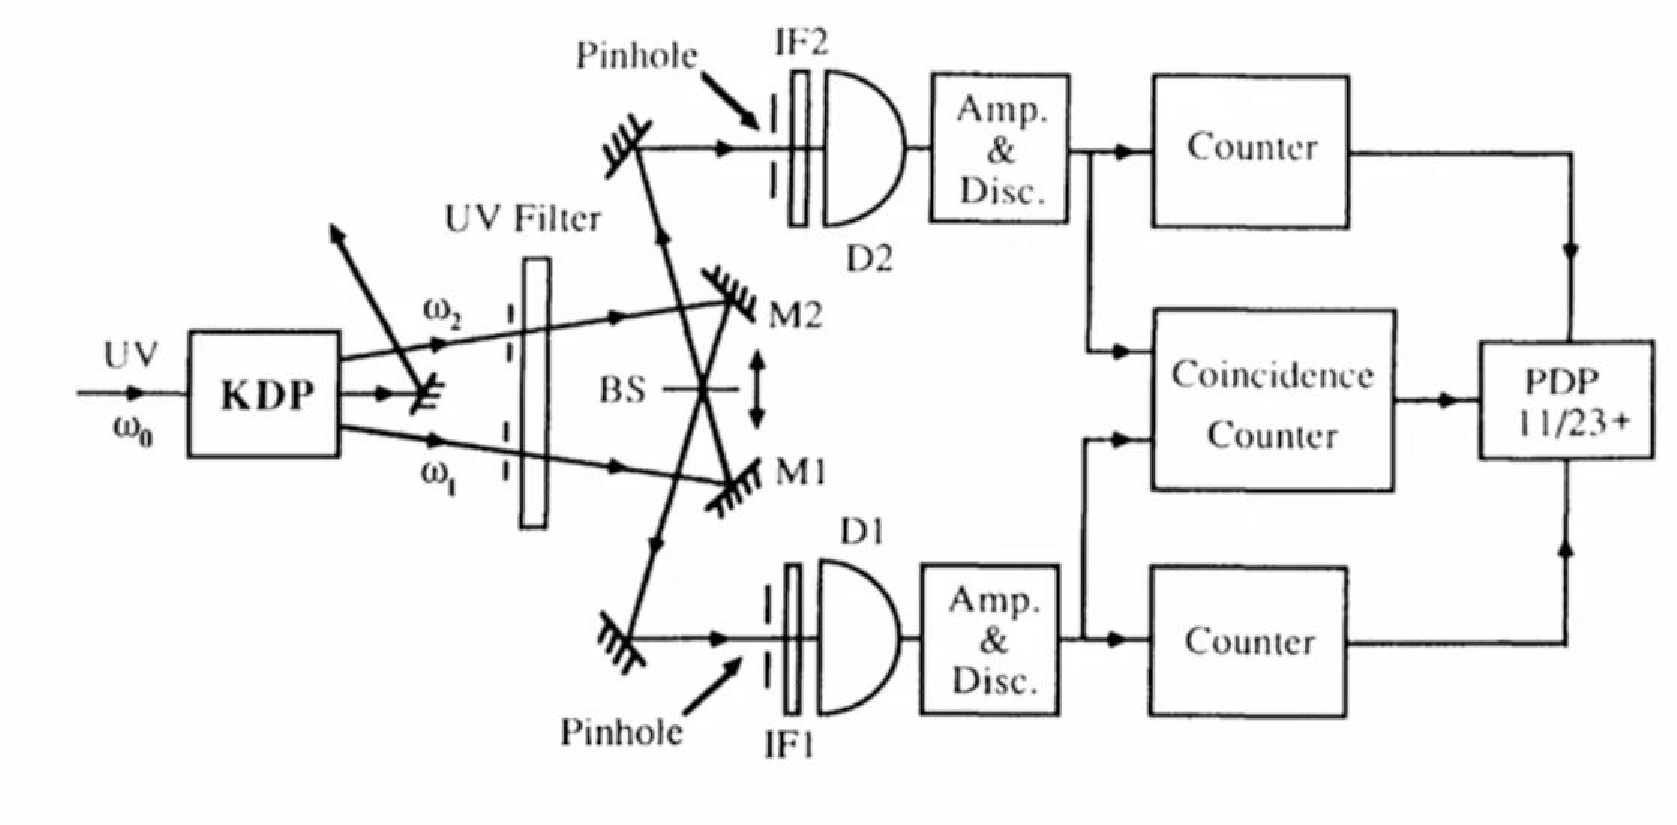
\includegraphics[width=0.9\linewidth]{images_in_pdf/16-/Grafico_90.pdf}
    \caption{Hong-Ou-Mandel interference set-up.}
    \label{fig:esempio}
\end{figure}

\begin{itemize}
    \item \hl{When $\Delta\tau = 0$}, the two wave packets overlap at the beam splitter and, if the photons are indistinguishable, the coincidence rate ideally drops to zero: this is the Hong--Ou--Mandel effect. This does not mean that the photons simply travel through one arm or the other in a classical sense; rather, \hl{the vanishing of coincidences is a genuine quantum interference effect arising from two indistinguishable two-photon amplitudes}, namely the case in which both photons are transmitted and the case in which both are reflected.
    
    \item \hl{For large delays, $|\Delta\tau| \gg \tau_c$}, where the coherence time is of order $\tau_c \sim 1/\Delta\omega$, \hl{the overlap between the two photons disappears}, the interference term vanishes, and the coincidence rate returns to the classical level: \hl{this happens because the two photons are no longer indistinguishable!}. For an ideal balanced beam splitter this corresponds to a normalized value of $1/2$.

\end{itemize}
\begin{figure}[H]
    \centering
    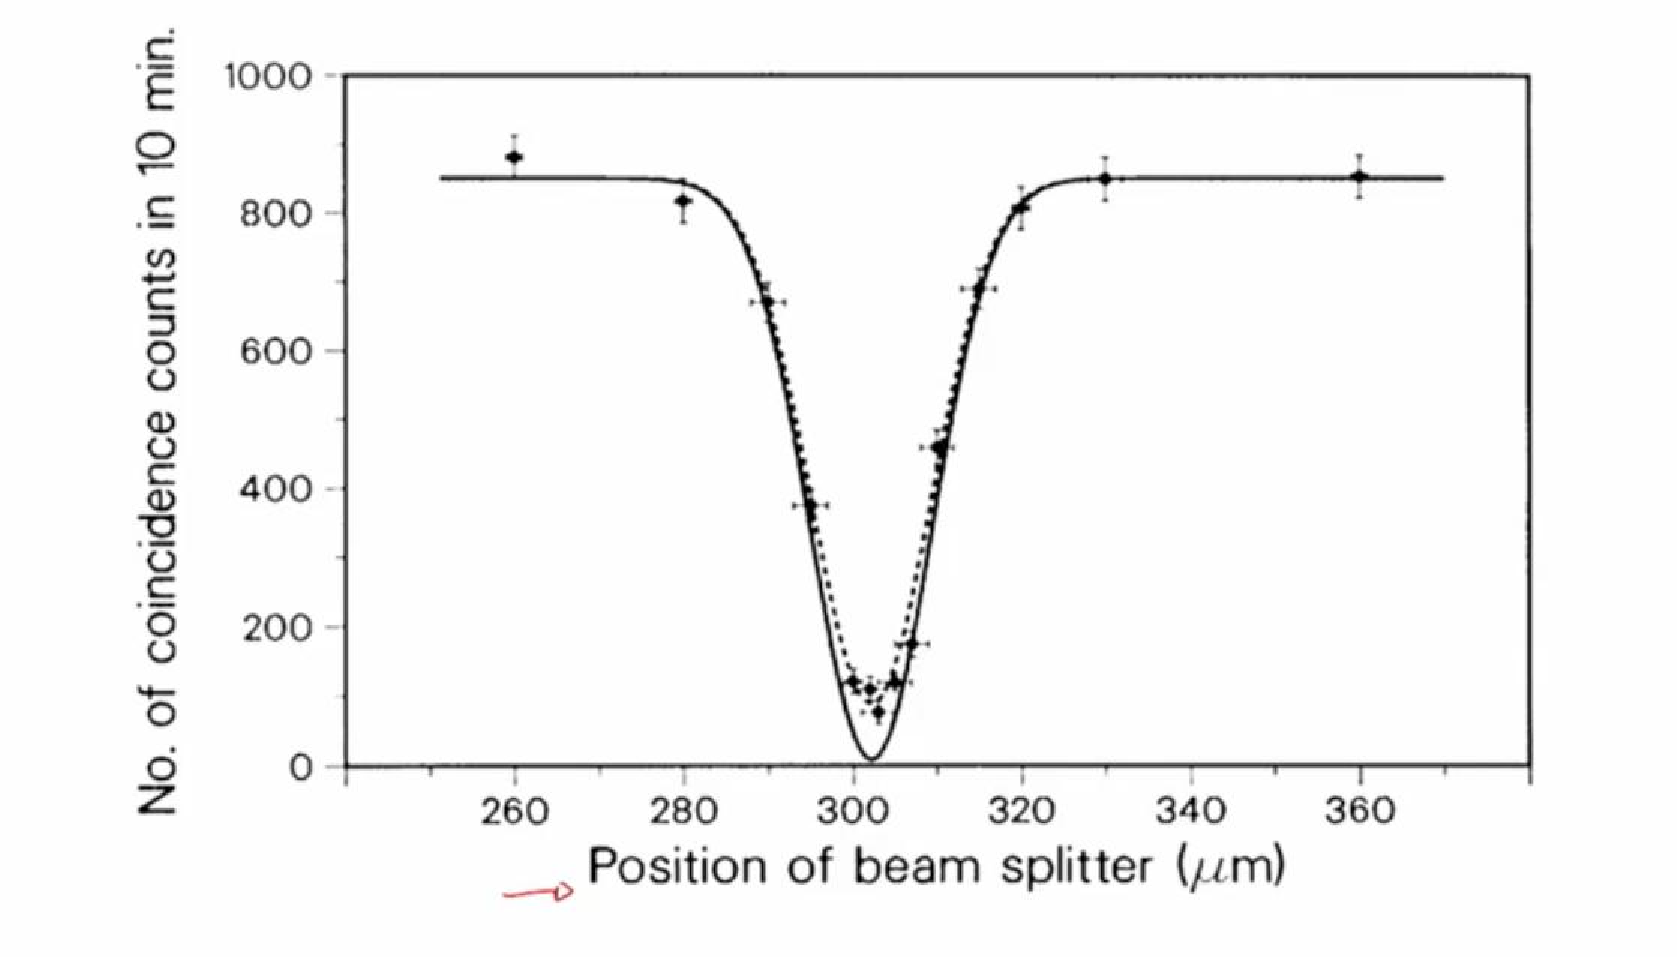
\includegraphics[width=0.9\linewidth]{images_in_pdf/16-/Grafico_91.pdf}
    \caption{Coincidence rate as a function of the relative delay $\Delta\tau$. The dip at zero delay is a signature of two-photon interference.}
    \label{fig:esempio2}
\end{figure}

\calloutinfo{%
    Notice that $\tau_c \approx ns$ which is difficult to measure by using time resolved detectors, by using this interferometer we can measure precisely the width of the dip which provides a direct measure of the temporal coherence of the photon wave packets.
}

\subsection{Quantum Eraser}

Suppose we consider the same system as before, but \hl{now we insert a half-wave plate along the idler arm}. This changes the polarization of the idler photon and, therefore, introduces a polarization tag that can carry which-path information:
\begin{figure}[H]
    \centering
    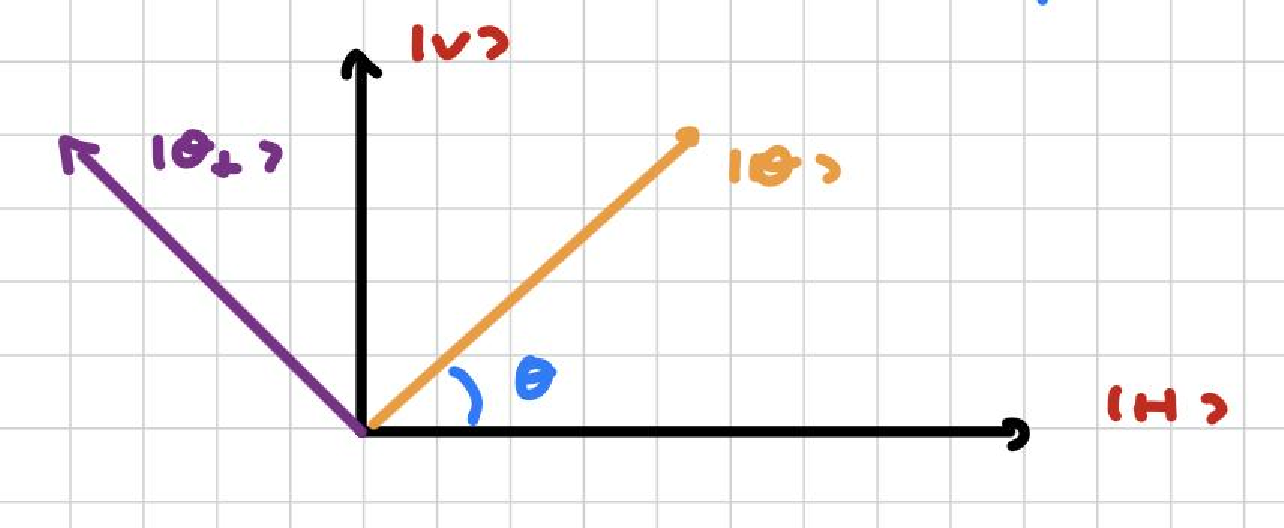
\includegraphics[width=0.6\linewidth]{images_in_pdf/16-/Grafico_92.pdf}
\end{figure}

\begin{equation}\label{eqn:16-polarization-states}
\ket{\theta}_i = 
\cos(\theta)\ket{H}_i + \sin(\theta)\ket{V}_i,
\qquad
\ket{\theta_\perp}_i = 
-\sin(\theta)\ket{H}_i + \cos(\theta)\ket{V}_i .
\end{equation}

If the original polarization of the signal photon is horizontal $\ket{H}$, the input state is no longer simply \(\ket{H}_s\ket{H}_i\), but rather
\begin{equation}\label{eqn:16-tagged-polarization}
    \ket{H}_s\ket{\theta}_i = \cos(\theta)\,\ket{H}_s\ket{H}_i + \sin(\theta)\, \ket{H}_s\ket{V}_i
\end{equation}

Using the same beam-splitter transformation as before, the output state is no longer the purely bunched two-photon state:
\begin{equation}\label{eqn:16-output-state}
    \ket{\psi}_{output} = \frac{i}{\sqrt{2}}\, \ket{0}_2\ket{2H}_3+\frac{i}{\sqrt{2}}\, \ket{2H}\ket{0}_3
\end{equation}

but instead becomes 
\begin{equation}\label{eqn:16-output-state-tagged}
\begin{split}
    \ket{\psi(\theta)}_{output} &= 
    \frac{i}{\sqrt{2}}\, \cos(\theta)\, 
    \bigl(
        \ket{2H}_2\ket{0}_3+\ket{0}_2\ket{2H}_3
    \bigr) + \\[0.5ex]
    &+\frac{1}{2}\, \sin(\theta)\, 
    \bigl(
        \ket{H}_2\ket{V}_3-\ket{V}_2\ket{H}_3
    \bigr) + \\[0.5ex]
    &+\frac{i}{2}\, \sin(\theta)\, 
    \bigl(
        \ket{H,V}_2\ket{0}_3-\ket{0}_2\ket{H,V}_3
    \bigr)
\end{split}
\end{equation}

\hl{When $\theta = \pi/2$, the idler photon becomes vertically polarized, while the signal photon remains horizontally polarized}. The two photons are therefore orthogonal in polarization and become distinguishable. The output state can be written as
\begin{equation}\label{eqn:16-output-state-orthogonal}
\Ket{\psi\!\left(\frac{\pi}{2}\right)}_{\text{output}}
=
\underbrace{\frac{1}{2}\bigl(\ket{H}_2\ket{V}_3-\ket{V}_2\ket{H}_3\bigr)}%
_{\Rnum{1}}
+
\underbrace{\frac{i}{2}\bigl(\ket{H,V}_2\ket{0}_3-\ket{0}_2\ket{H,V}_3\bigr)}%
_{\Rnum{2}}.
\end{equation}

\begin{enumerate}
    \item The first term ($\Rnum{1}$) describes events in which the two photons exit through different output ports, leading to coincidence detections;
    \item The second term ($\Rnum{2}$) corresponds to both photons exiting through the same output port with orthogonal polarizations. 
\end{enumerate}

\calloutwarn{%
Since the photons are distinguishable, the two-photon interference responsible for the Hong--Ou--Mandel effect is no longer complete, and \textbf{coincidence counts reappear}.

Physically, \textbf{the polarization degree of freedom carries which-path information}, allowing one in principle to distinguish the two photons, thereby reducing the destructive interference. 
} 

\begin{figure}[H]
    \centering
    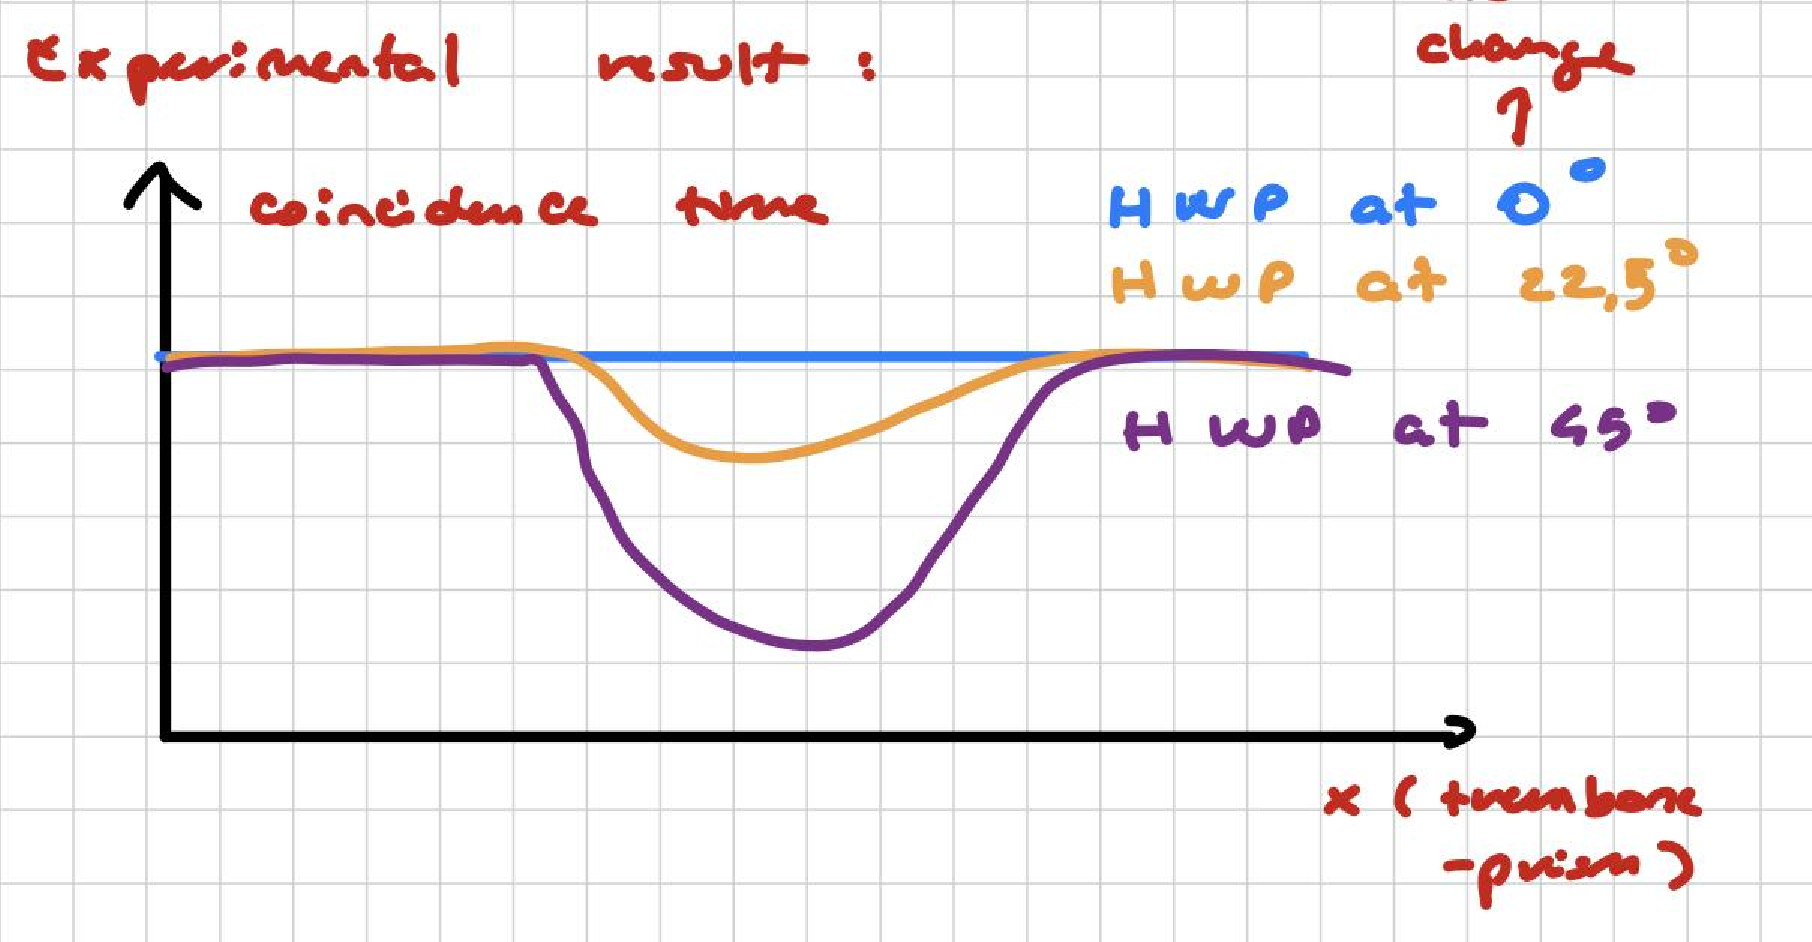
\includegraphics[width=0.6\linewidth]{images_in_pdf/16-/Grafico_93.pdf}
\end{figure}
\textbf{However}, \hl{the information is erased if both output beams are projected onto the same polarization basis by placing polarizers before the detectors} with $\theta_a$ and $\theta_b$. In that case, the coincidence probability becomes
\begin{equation}\label{eqn:16-coincidence-probability-erased}
P = \left|\bra{\theta_a}\braket{\theta_b | \psi_{\text{output}}}\right|^2
= \frac{1}{4}\sin^2(\theta_b-\theta_a),
\end{equation}

so that $P\to 0$ when $\theta_a=\theta_b$.

This restores indistinguishability in the selected sub-ensemble and is the essence of the quantum eraser.
\begin{figure}[H]
    \centering
    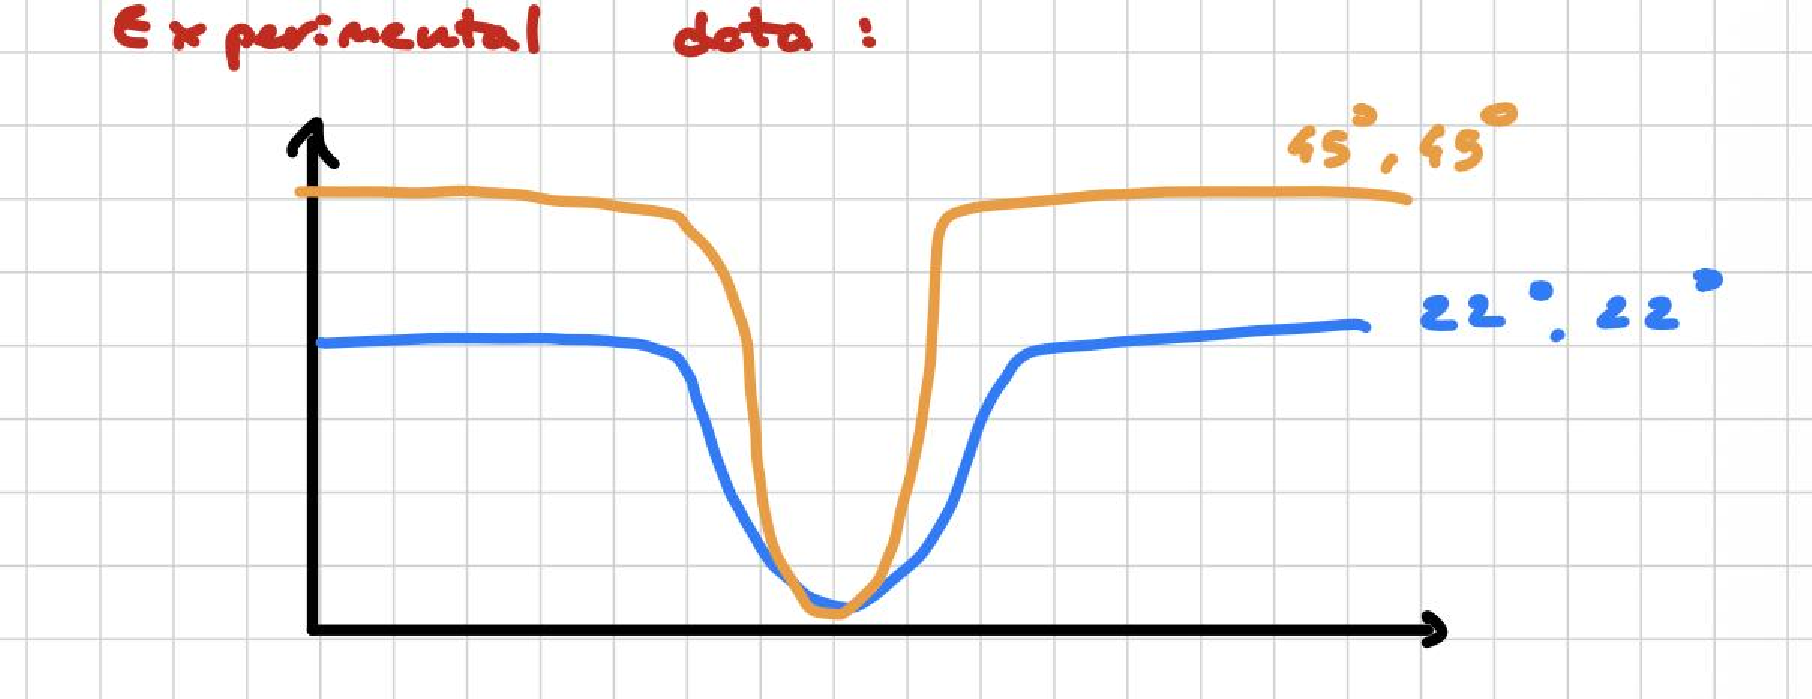
\includegraphics[width=0.6\linewidth]{images_in_pdf/16-/Grafico_94.pdf}
    \caption{Intensity measurements at \qty{45}{\degree} and \qty{22}{\degree}}
\end{figure}

\subsection{Application of entanglement to interferometry}
Classically, the measurement of the difference photocurrent in an interferometer exhibits a sinusoidal fringe pattern when a phase shift is introduced by an optical element in one arm. 

\begin{figure}[H]
    \centering
    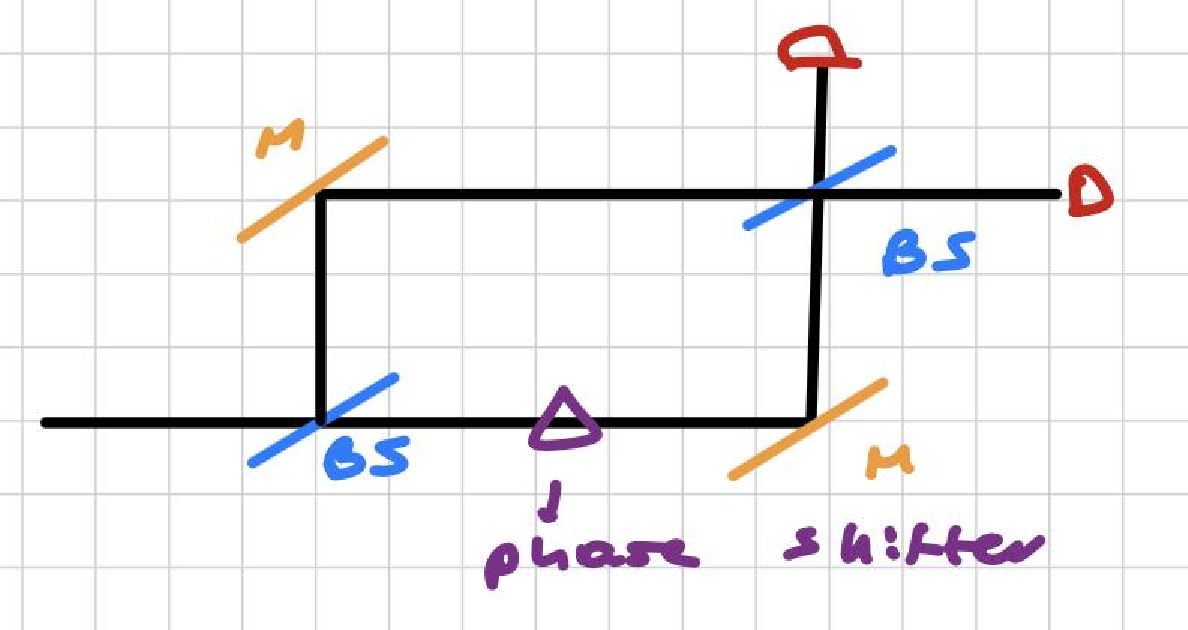
\includegraphics[width=0.6\linewidth]{images_in_pdf/16-/Grafico_95.pdf}
\end{figure}

The accuracy of the phase measurement $\Delta\theta$ is limited by photocurrent fluctuations, namely shot noise. For an input beam with mean photon number $\bar n$, the standard quantum limit gives
\begin{equation}\label{eqn:16-shot-noise-limit}
\Delta\theta \sim \frac{1}{\sqrt{\bar n}}.
\end{equation}

As in applications such as gravitational-wave detection, the \hl{phase sensitivity can be improved by using non-classical light}. Consider now one photon entering each input port of the first beam splitter:
\begin{figure}[H]
    \centering
    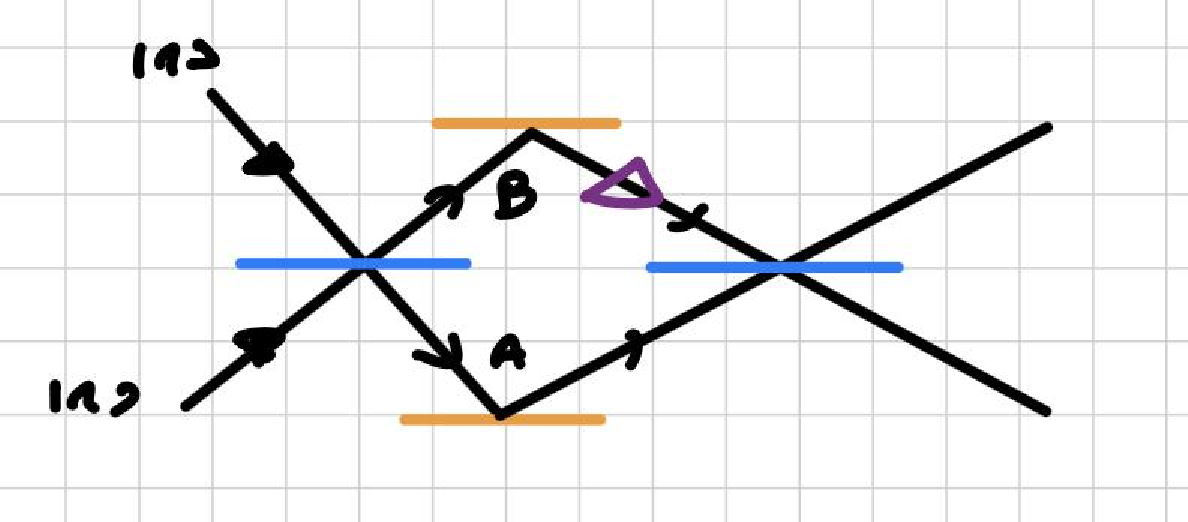
\includegraphics[width=0.6\linewidth]{images_in_pdf/16-/Grafico_96.pdf}
    \caption{Path-entangled photons}
\end{figure}

After the first beam splitter, one obtains a path-entangled state (up to a convention-dependent phase),
\begin{equation}\label{eqn:16-path-entangled-state}
\frac{1}{\sqrt{2}}\left(\ket{2}_A\ket{0}_B+\ket{0}_A\ket{2}_B\right).
\end{equation}

Since \hl{a phase shifter is placed before the second beam splitter}, the state becomes
\begin{equation}
\frac{1}{\sqrt{2}}\left(\ket{2}_A\ket{0}_B+e^{2i\theta}\ket{0}_A\ket{2}_B\right),
\end{equation}

because \hl{both photons in the same arm acquire the phase shift}n. After the second beam splitter, the output state can be written as
\begin{equation}
\ket{\psi}_{\text{output}}
=
\frac{1}{2\sqrt{2}}\left(1-e^{2i\theta}\right)
\left(\ket{2}_A\ket{0}_B-\ket{0}_A\ket{2}_B\right)
+\frac{i}{2}\left(1+e^{2i\theta}\right)\ket{1}_A\ket{1}_B,
\end{equation}

up to an overall global phase and depending on the beam-splitter convention. It can be shown that the phase sensitivity of this ideal two-photon entangled state is
\begin{equation}\label{eqn:16-phase-sensitivity}
\Delta\theta = \frac{1}{2},
\end{equation}

\hl{which is better than the shot-noise limit for a coherent state with the same mean photon number $\bar n = 2$}, namely
\begin{equation}\label{eqn:16-shot-noise-limit-2}
\Delta\theta \simeq \frac{1}{\sqrt{2}}.
\end{equation}

This means that \hl{the phase resolution is improved}. 

\calloutinfo{%
    The advantage does not come from a classical (\emph{phase squeezed}) coherent state, but from the entanglement generated inside the interferometer.
}

The natural generalization to $N$ photons is referred to as the \textbf{NOON state}:
\begin{equation}\label{eqn:16-noon-state}
\ket{\psi}=\frac{1}{\sqrt{2}}\left(\ket{N}_A\ket{0}_B+e^{i\phi_N}\ket{0}_A\ket{N}_B\right),
\end{equation}

which leads, in the ideal case, to the Heisenberg scaling
\begin{equation}\label{eqn:16-heisenberg-scaling}
\Delta\theta \sim \frac{1}{N}.
\end{equation}

\calloutwarn{%
    These states are extremely useful, but also difficult to realize experimentally: a single beam splitter can generate the two-photon case, whereas larger-\(N\) NOON states require more elaborate schemes. Moreover, their detection generally demands photon-number-resolving detectors, which are technically demanding because they must distinguish different photon numbers with high efficiency and low noise.
}

\subsection{Quantum teleportation}

\emph{Quantum teleportation} is an application of entanglement where the key point is to transfer information and not matter. In practice, we have a particle in a particular quantum state that we want to teleport to another particle at a distant location. This need specific conditions:
\begin{enumerate}
    \item A \hl{classical communication channel};
    \item Entanglement.
\end{enumerate}

\subsubsection{Qubits and Bell states}

We consider as basic unit of information the \textbf{qubit}: that can be represented as a normalized superposition of states $\ket{0}$ and $\ket{1}$. For a generic two-level system:
\begin{equation}
    \ket{\psi} = a\, \ket{0}+b\, \ket{1}; \hspace{2ex} a,b \in \mathbb{C}; \hspace{2ex} |a|^2+|b|^2 = 1.
\end{equation}

Using spherical coordinates:
\begin{equation}
    \ket{\psi} = \cos\left(\tfrac{\theta}{2}\right) \, \ket{0}+ 
    e^{i\phi}\, \sin\left(\tfrac{\theta}{2}\right) \, \ket{1};
    \hspace{2ex} 0\leq \theta \leq \pi;
    \hspace{2ex} 0\leq \phi\leq 2\pi.
\end{equation}

A state like this can be represented on an unitary sphere called \textbf{Bloch Sphere} 
\begin{figure}[H]
    \centering
    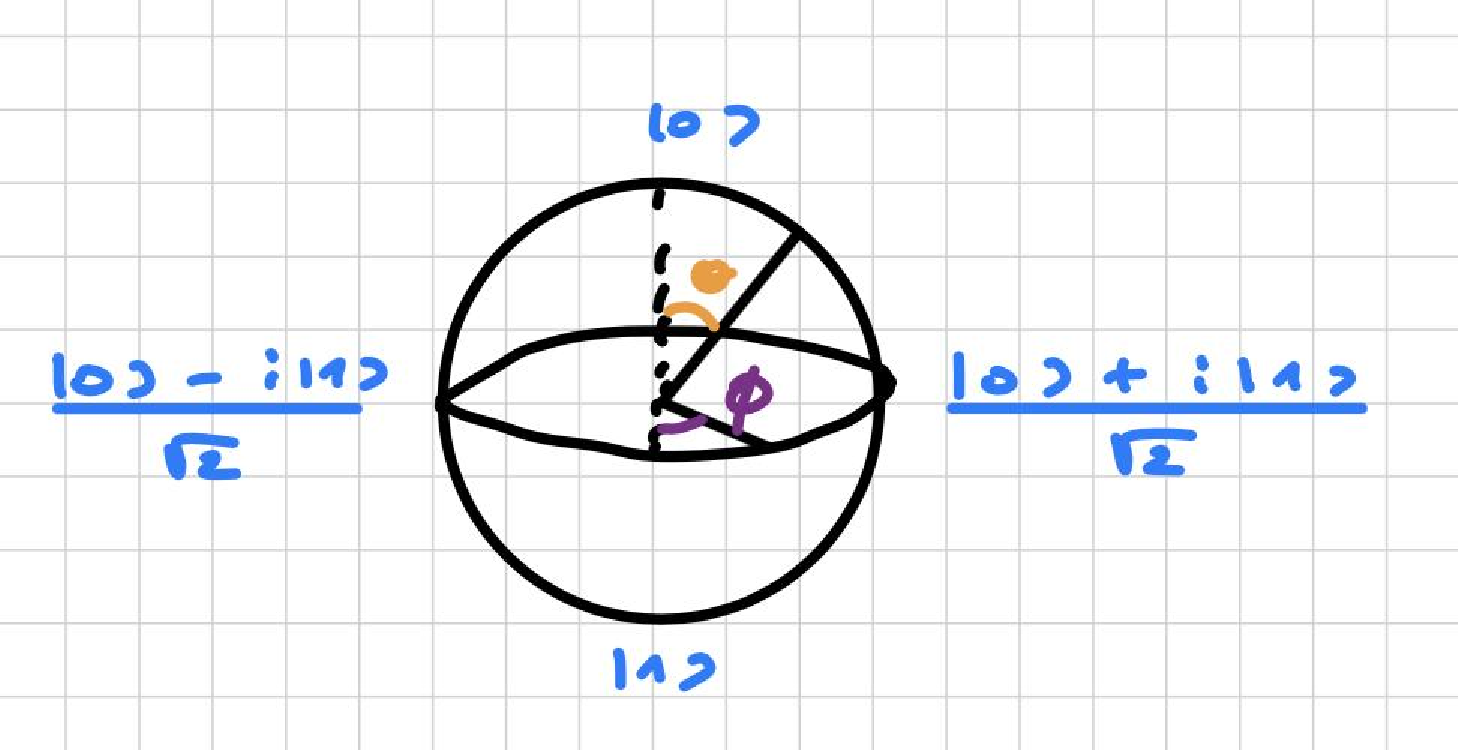
\includegraphics[width=0.6\linewidth]{images_in_pdf/16-/Grafico_97.pdf}
    \caption{Bloch sphere}
\end{figure}

\hl{We will interpret $\ket{0}$ and $\ket{1}$ as our polarized states $\ket{H}$ and $\ket{V}$}. In classical optics we have an unitary sphere to represent polarized states called \textbf{Poincaré sphere}: 
\begin{figure}[H]
    \centering
    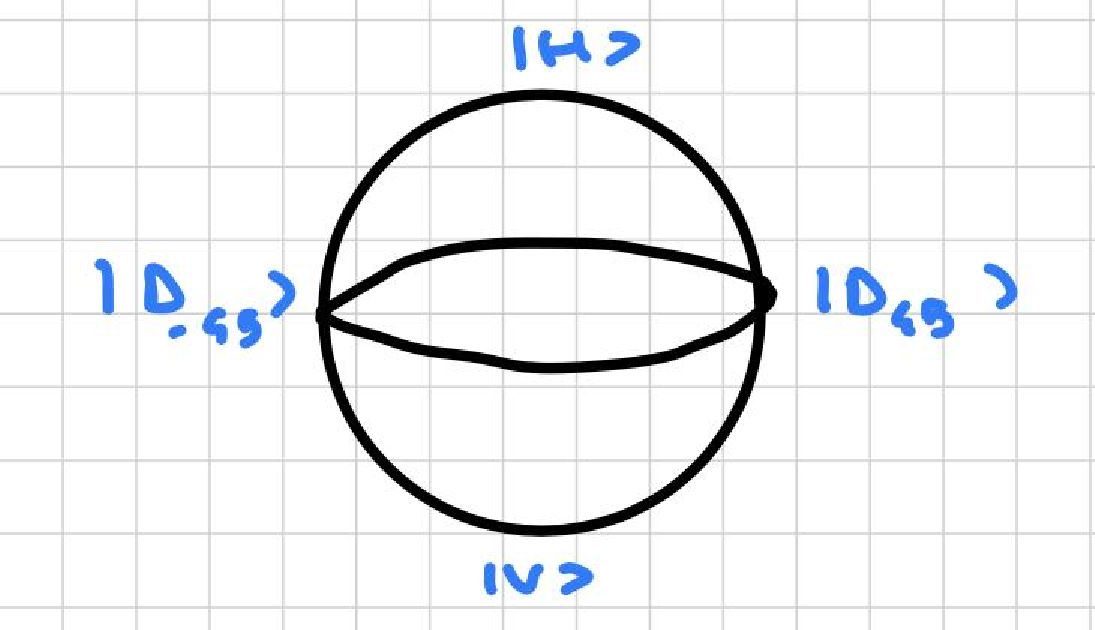
\includegraphics[width=0.6\linewidth]{images_in_pdf/16-/Grafico_98.pdf}
    \caption{Poincaré sphere}
\end{figure}

In this way, 2 bits become 2 qubits:
\begin{equation}\label{eqn:16-two-qubits-state}
00,01,10,11 \implies \ket{\psi} = a\, \ket{0}\ket{0}+ b\, \ket{0}\ket{1}+ c\, \ket{1}\ket{0}+ d\, \ket{1}\ket{1}
\end{equation}

A frequently used set of 2 qubits states are the \textbf{Bell states}, both entangled:
\begin{equation}\label{eqn:16-bell-states}
\ket{\phi^{\pm}} = 
\frac{1}{\sqrt{2}}\, 
\bigl(
    \ket{0}\ket{0}\pm \ket{1}\ket{1}
\bigr)
\hspace{2ex} \land \hspace{2ex}
\ket{\psi^{\pm}} =
\frac{1}{\sqrt{2}}\, 
\bigl(
    \ket{0}\ket{1}\pm \ket{1}\ket{0}
\bigr)
\end{equation}

We need to remember two important things:
\begin{enumerate}
    \item Classical information channels implies that the information can't be faster than the speed of light velocity $C$;
    
    \item We need to remember that there is the \textbf{no cloning theorem}.
\end{enumerate}

\begin{figure}[H]
    \centering
    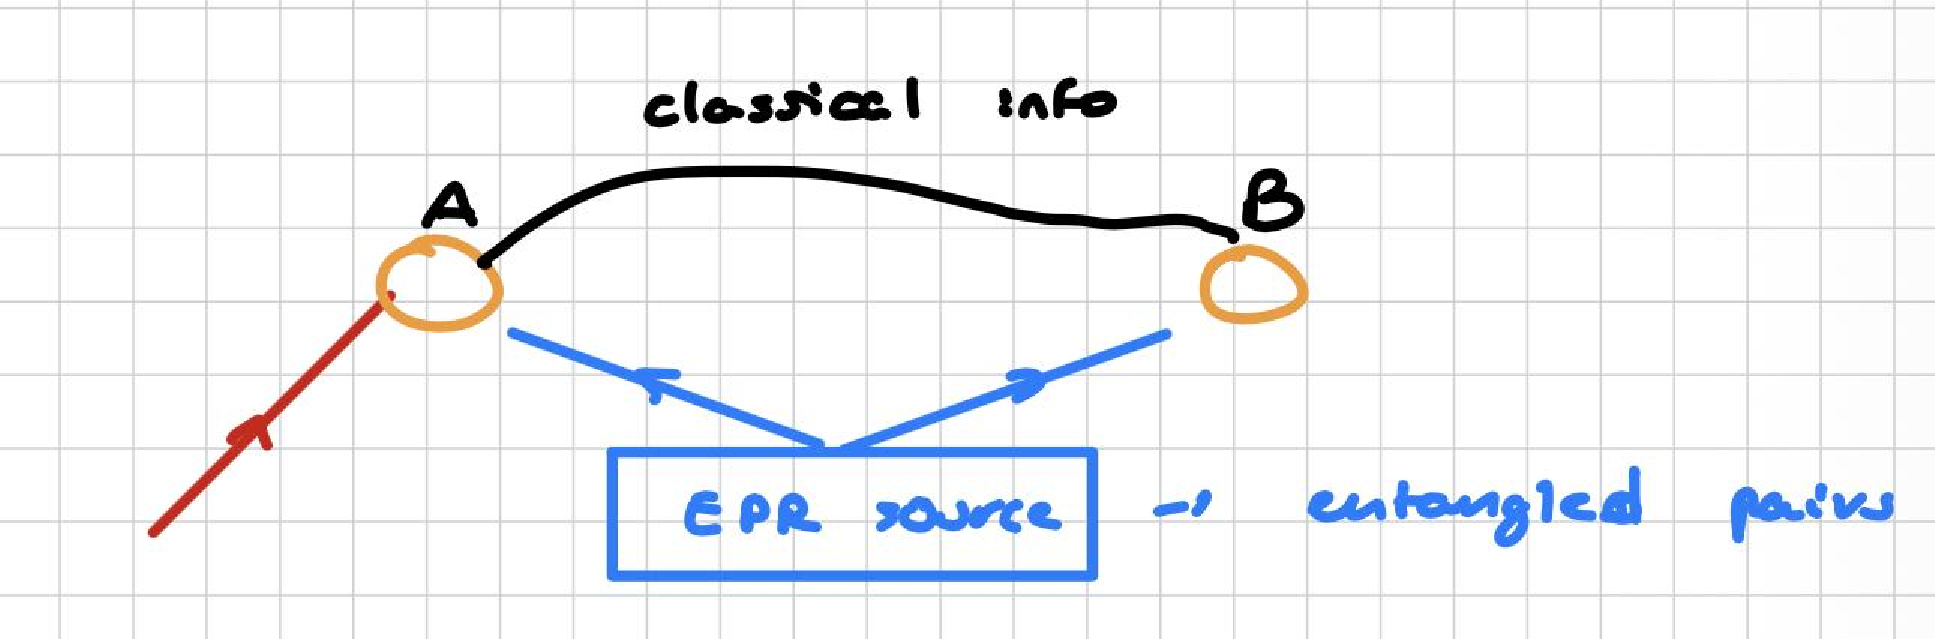
\includegraphics[width=0.6\linewidth]{images_in_pdf/16-/Grafico_99.pdf}
    \caption{Simple scheme of the teleportation protocol}
\end{figure}

\subsubsection{Teleportation protocol}

Suppose Alice has a photon in a particular state $\ket{\psi_A}$ that she wants to teleport to Bob:
\begin{equation}\label{eqn:16-teleportation-initial-state}
\ket{\psi_A} =c_0\, \ket{0}_A +c_1 \, \ket{1}_A.
\end{equation}

In the following, kets will always indicate -- by pedice $A$ or $B$ -- their respective owner. Alice may not know $c_0$ and $c_1$, but she can communicate with Bob through a classical channel. Then \hl{we have a EPR source which send separately entangled photons to Alice and Bob}:
\begin{equation}\label{eqn:16-epr-source}
\ket{\varphi_{AB}} =\frac{1}{\sqrt{2}}\, 
\bigl(
    \ket{0}_A\ket{0}_B+\ket{1}_A\ket{1}_B
\bigr).
\end{equation}

We consider the 3-photon state as:
\begin{equation}\label{eqn:16-teleportation-initial-state-2}
\ket{\Psi} = \ket{\varphi_{AB}}\,\ket{\psi_A} = 
\frac{1}{\sqrt{2}}\, 
\bigl(
    \ket{0}_A\ket{0}_B+\ket{1}_A\ket{1}_B
\bigr)
\, 
\bigl(
    c_0\, \ket{0}_A +c_1 \, \ket{1}_A
\bigr)
\end{equation}

If we consider the Bell (already defined in Equation \ref{eqn:16-bell-states}) states only using Alice's photons:
\begin{equation}\label{eqn:16-bell-states-alice}
\ket{\phi^{\pm}}_{AA} = 
\frac{1}{\sqrt{2}}\, 
\bigl(
    \ket{0}_A\ket{0}_A\pm\ket{1}_A\ket{1}_A
\bigr) 
\hspace{2ex} \land \hspace{2ex}
\ket{\psi^{\pm}}_{AA} = 
\frac{1}{\sqrt{2}}\, 
\bigl(
    \ket{0}_A\ket{1}_A\pm\ket{1}_A\ket{0}_A
\bigr) 
\end{equation}

Using them we can rewrite the \textbf{total 3-qubit state} as:
\begin{align}
\ket{\Psi} &= 
\ket{\psi}_A \otimes \ket{\varphi}_{AB} = \nonumber \\[0.5ex]
&= \frac{1}{\sqrt{2}} 
\bigl[ 
    c_0\ket{0}_A\ket{0}_A\ket{0}_B + 
    c_0\ket{0}_A\ket{1}_A\ket{1}_B + \nonumber \\[0.5ex]
    &\qquad +
    c_1\ket{1}_A\ket{0}_A\ket{0}_B +
    c_1\ket{1}_A\ket{1}_A\ket{1}_B 
\bigr] = \nonumber \\[0.5ex]
&= \frac{1}{2} 
\bigl[ 
    \ket{\phi^+}_{AA} 
    \left(c_0\ket{0}_B + c_1\ket{1}_B\right) + 
    \ket{\phi^-}_{AA}
    \left(c_0\ket{0}_B - c_1\ket{1}_B\right) + \nonumber \\[0.5ex]
    &\qquad + 
    \ket{\psi^+}_{AA} 
    \left(c_0\ket{1}_B + c_1\ket{0}_B\right) +
    \ket{\psi^-}_{AA} 
    \left(c_0\ket{1}_B - c_1\ket{0}_B\right) 
\bigr]. \label{eqn:quantum-teleportation-algebra}
\end{align}

\calloutinfo{%}
Notice that Alice and Bob have sufficient information to write this expression. To any possible outcome of Alice's measurement, there is a corresponding state of Bob's photon. The measurement on Alice's side constrains the state of Bob's photon into one of four possible states, each related to Alice's original state $\ket{\psi_A}$ by a known unitary transformation.
}

\subsubsection{Teleportation protocol: all possible scenarios unpacked}

In the following, we unpack all the possible scenarios after Alice performs a measurement on the Bell basis:
\begin{enumerate}
    \item \textbf{Alice obtains $\ket{\phi^+}$}: after projecting on the ket, Bob will obtain a copy of Alice's initial photon state:
    \begin{equation}\label{eqn:16-bob-state-alice-phi-plus}
        c_0\, \ket{0}_B+c_1\, \ket{1}_B
    \end{equation}

    Alice communicates to Bob -- through the classical channel -- her result and \hl{Bob instantly knows his photon is in state $\ket{\psi_A}$ without needing to measure the state}, so we actually made the teleportation.

    \item \textbf{Alice obtains $\ket{\phi^-}$}: after projecting on the ket, Alice tells her measurement result to Bob; he will immediately know that his photon is in the state:
    \begin{equation}\label{eqn:16-bob-state-alice-phi-minus}
        c_0\, \ket{0}_B-c_1\, \ket{1}_B
    \end{equation}

    To resolve it Bob changes the sign by applying a \textbf{unitary operation} to his photon; this is a \hl{polarization rotation by a half-wave plate}:
    \begin{equation}\label{eqn:16-bob-state-alice-phi-minus-transformation}
        \ket{0}_B \to \ket{0}_B \hspace{1cm} \ket{1}_B \to -\ket{1}_B
    \end{equation}
    
    \item \textbf{Alice obtains $\ket{\psi^+}$}: after projecting on the ket, Bob will know that his photon is in the state:
    \begin{equation}\label{eqn:16-bob-state-alice-psi-plus}
        c_0\, \ket{1}_B+c_1\, \ket{0}_B
    \end{equation}

    To resolve it Bob changes the sign by applying a \textbf{unitary operation} to his photon:
    \begin{equation}\label{eqn:16-bob-state-alice-psi-plus-transformation}
        \ket{1}_B \to \ket{0}_B \hspace{1cm} \ket{0}_B \to \ket{1}_B
    \end{equation}

    \item \textbf{Alice obtains $\ket{\psi^-}$}: after projecting on the ket, Bob will know that his photon is in the state:
    \begin{equation}\label{eqn:16-bob-state-alice-psi-minus}
        c_0\, \ket{1}_B-c_1\, \ket{0}_B
    \end{equation}

    To resolve it Bob changes the sign by applying a \textbf{unitary operation} to his photon:
    \begin{equation}\label{eqn:16-bob-state-alice-psi-minus-transformation}
        \ket{1}_B \to \ket{0}_B \hspace{1cm} \ket{0}_B \to -\ket{1}_B
    \end{equation}

\end{enumerate}

All the beforehand mentioned operations are $2\times2$ unitary matrices; it is possible to show that such matrices are generated by a four-element set $\left\{ \identity, \sigma_x,\sigma_y,\sigma_z\right\}$ comprising Pauli matrices and the identity matrix:
\begin{equation}\label{eqn:16-span-pauli-matrices}
    U = 
    \alpha_1 \sigma_x + \alpha_2 \sigma_y + \alpha_3 \sigma_z + \beta \identity
    \equiv
    \vec{\alpha} \cdot \vec{\sigma} + \beta \identity;
    \hspace{2ex}
    \forall\,
    U\ s.t.\ U^\dagger = U^{-1};
    \hspace{2ex}
    \vec{\alpha}\in\mathbb{C}^3,\, \beta\in\mathbb{C}.
\end{equation}

\calloutinfo{%}
    Notice that \textbf{there is no violation of the no-cloning theorem}, because the Bell-state \textbf{measurement destroys the original state} during the teleportation process.
}

\subsection{Experimental setup of the Innsbruck group}
The experiment starts with a UV pump beam exciting a nonlinear crystal, which acts as an EPR source and produces an entangled photon pair, this time labelled 2 and 3, in the Bell state
\begin{equation}\label{eqn:16-innsbruck-epr-pair}
\ket{\psi^-}_{2,3}=\frac{1}{\sqrt{2}}
\left(\ket{H}_2\ket{V}_3-\ket{V}_2\ket{H}_3\right).
\end{equation}

In this state, the two photons do not have a definite polarization individually, but only as a joint system. A second UV pump beam, reflected by a mirror, generates another photon pair; one photon is used as a trigger to synchronize the experiment, while the other -- referred to as photon 1 -- is prepared in an arbitrary polarization state,
\begin{equation}\label{eqn:16-innsbruck-state-to-teleport}
\ket{\psi}_1 =
\alpha\ket{0}_1+\beta\ket{1}_1,
\end{equation}

which is the unknown state to be teleported. Alice then performs a Bell-state measurement on photons 1 and 2 by sending them to a beam splitter followed by two detectors.
\begin{figure}[H]
    \centering
    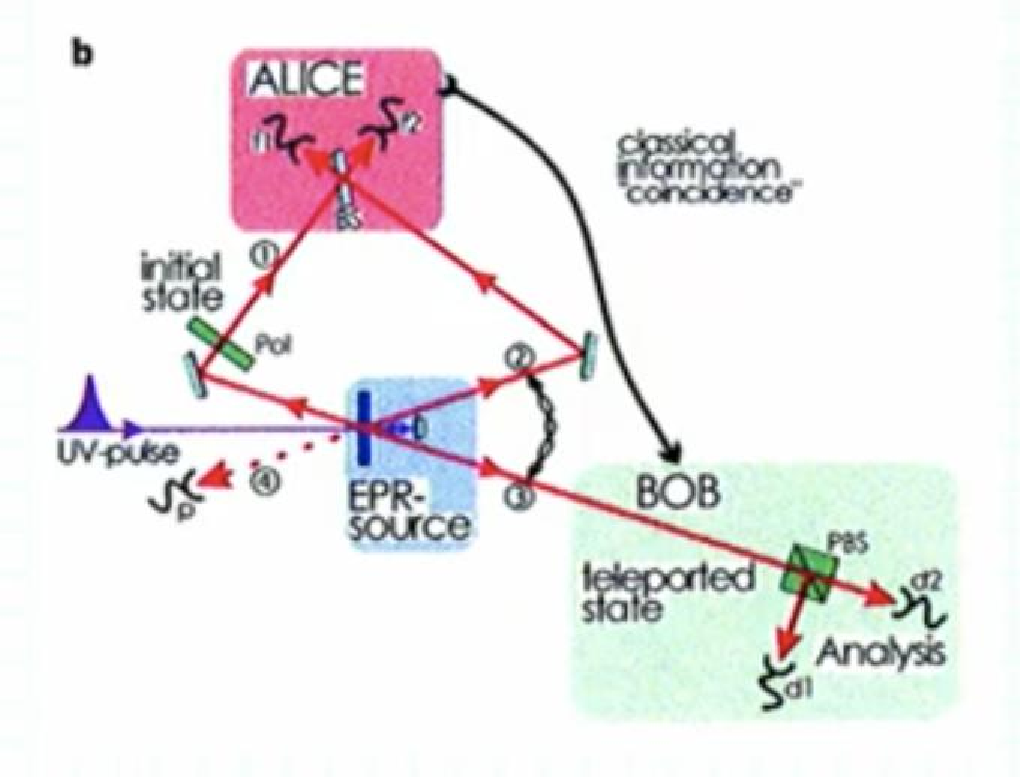
\includegraphics[width=0.6\linewidth]{images_in_pdf/16-/Grafico_100.pdf}
    \caption{Experimental setup for teleportation of the Innsbruck group.}
\end{figure}

\hl{In this implementation, the Bell state $\ket{\psi^-}_{1,2}$ is the easiest one to identify, because it \textbf{is the only state that produces coincidence counts} at the two detectors after the beam splitter}, whereas the other Bell states are symmetric under exchange and therefore lead to bunching at the same output port. The reason is that $\ket{\psi^-}_{1,2}$ is \textbf{antisymmetric under particle exchange}, so the two photons must exit through different output ports, giving simultaneous clicks. If Alice detects $\ket{\psi^-}_{1,2}$, then photon 3 is projected onto the same state that photon 1 initially carried, up to a known phase depending on the chosen convention,
\begin{equation}\label{eqn:16-innsbruck-teleported-state}
\ket{\psi}_3 \sim
\alpha \ket{0}_B+ \beta \ket{1}_B.
\end{equation}

In this sense, the Bell-state measurement destroys the identity of photon 1 during the process, so the state is not copied but transferred to Bob's photon, in full agreement with the no-cloning theorem. \hl{The key point is that photons 2 and 3 were initially prepared in the entangled state $\ket{\psi^-}_{2,3}$}, so the measurement on photons 1 and 2 effectively teleports the quantum information from photon 1 to photon 3. 

\calloutinfo{%
    Bob can then verify the success of the teleportation by analyzing the polarization of his photon with a polarizing beam splitter set at $+45^\circ$ and $-45^\circ$, and by measuring the corresponding coincidence counts at detectors $D_3$ and $D_4$.
}

Further readings are: \cite{art:Ursin-2007-144km-teleportation}, \cite{art:Wang-2017-ground-to-satellite} and \cite{art:Yin-2020-entanglement-based-crypto}.

\subsection{Entanglement swapping}

At this stage we only know how to create entanglement between photons generated by the same source.

\question{Can entanglement also be distributed between particles that come from different sources and have never interacted?}{%
The answer is yes: this is the idea of \textbf{entanglement swapping}. A Bell-state measurement on two photons can transfer entanglement to the remaining two photons, even if they are far apart and originate from independent sources.
}

We consider two different EPR sources emitting the entangled pairs $(1,2)$ and $(3,4)$. The four-photon state is
\begin{equation}\label{eqn:16-entanglement-swapping-epr-pairs-couple}
\ket{\psi}_{1,2,3,4}
=
\frac{1}{2}
\bigl(\ket{H}_1\ket{V}_2-\ket{V}_1\ket{H}_2\bigr)
\otimes
\bigl(\ket{H}_3\ket{V}_4-\ket{V}_3\ket{H}_4\bigr).
\end{equation}

The first factor describes the entanglement between photons 1 and 2, while the second factor describes the entanglement between photons 3 and 4. Their product means that there is initially no entanglement between the two pairs.
\begin{figure}[H]
    \centering
    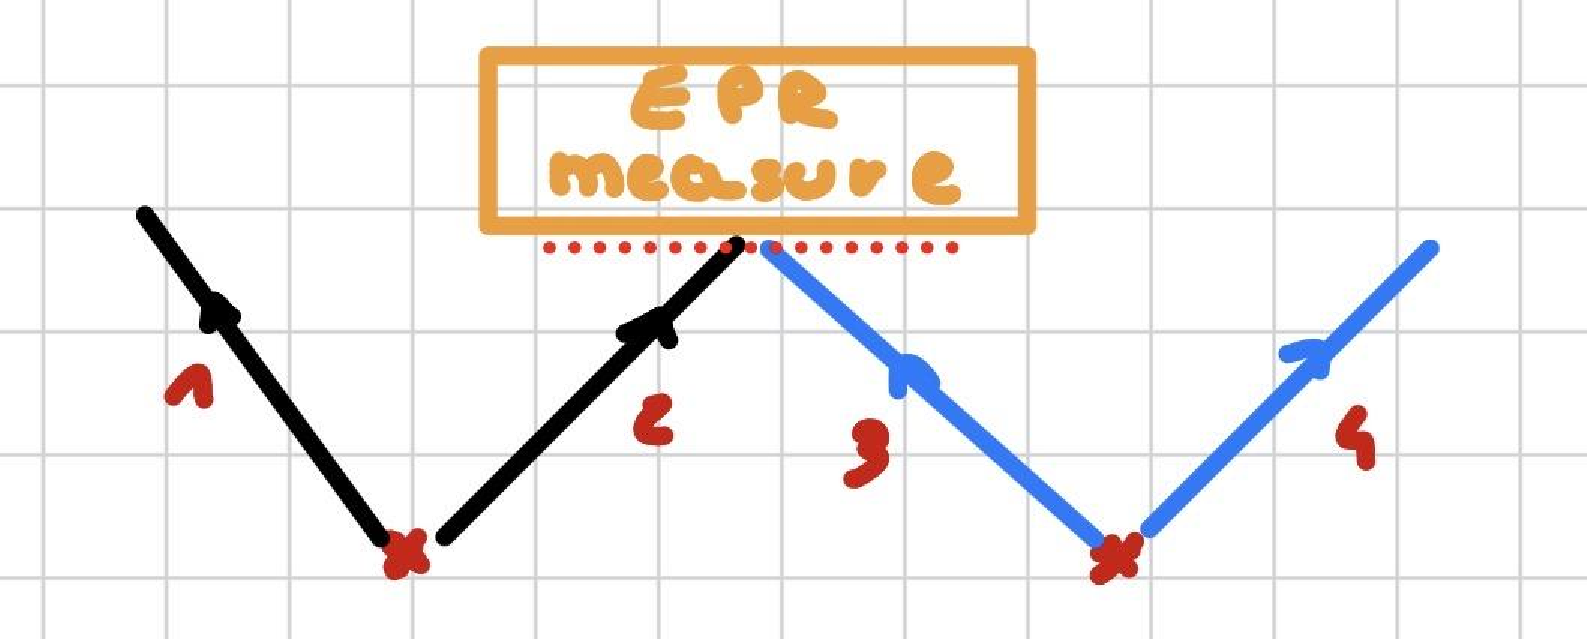
\includegraphics[width=0.6\linewidth]{images_in_pdf/16-/Grafico_101.pdf}
    \caption{Scheme of entanglement swapping in a quantum repeater.}
\end{figure}

The Bell states of photons 2 and 3 are
\begin{align}
\ket{\psi^{\pm}}_{2,3}
&= \frac{1}{\sqrt{2}}
\bigl(
    \ket{H}_2\ket{V}_3\pm\ket{V}_2\ket{H}_3
\bigr),
\\
\ket{\phi^{\pm}}_{2,3}
&= \frac{1}{\sqrt{2}}
\bigl(
    \ket{H}_2\ket{H}_3\pm\ket{V}_2\ket{V}_3
\bigr).
\end{align}

Using these definitions, the initial four-photon state can be rewritten as
\[
\ket{\psi}_{1,2,3,4} = \frac{1}{2}\, \left(\ket{\psi^+}_{1,4}\ket{\psi^+}_{2,3}+\ket{\psi^-}_{1,4}\ket{\psi^-}_{2,3}+\ket{\phi^+}_{1,4}\ket{\phi^+}_{2,3}+\ket{\phi^-}_{1,4}\ket{\phi^-}_{2,3}\right)
\]

\calloutinfo{%
    Therefore, a Bell-state measurement on photons 2 and 3 projects photons 1 and 4 onto the corresponding Bell state. In particular, if photons 2 and 3 are found in the state $\ket{\psi^-}_{2,3}$, then photons 1 and 4 are projected onto \(\ket{\psi^-}_{1,4}\). \textbf{This means that entanglement has been swapped}: photons 1 and 4 become entangled even though they never interacted directly.
}

Notice that we need to fulfill specific conditions:
\begin{itemize}
    \item They come from different sources;
    \item They never interacted ;
    \item The entangled state of 1 and 4 is exactly the same of the entangled state 2 and 3.
\end{itemize}

\textbf{Experimentally}, \hl{one looks for coincidences between the detectors $D_1^\dagger $ and $D_4$, or between $D_1^-$ and $D_4$}, conditioned on the detection of $\ket{\psi^-}_{2,3}$. Photon 1 is analyzed along the $+45^\circ$ and $-45^\circ$ bases, while photon 4 is analyzed at a variable polarization angle $\theta$. \hl{If entanglement swapping occurs, the coincidence rate for one analyzer setting reaches a minimum while the complementary setting reaches a maximum}, exactly as expected for an entangled Bell pair.

Looking at the coincidence rates as a function of $\theta$ in Figure \ref{16-entanglement-swapping}, one finds that:
\begin{itemize}
    \item $D_1^\dagger -D_4$ coincidence rate for  $\theta =+ 45^\circ\implies $ is Min
    \item $D_1^--D_4$ coincidence rate for  $\theta =+ 45^\circ\implies $ is Max 
\end{itemize}

\begin{figure}[H]
    \centering
    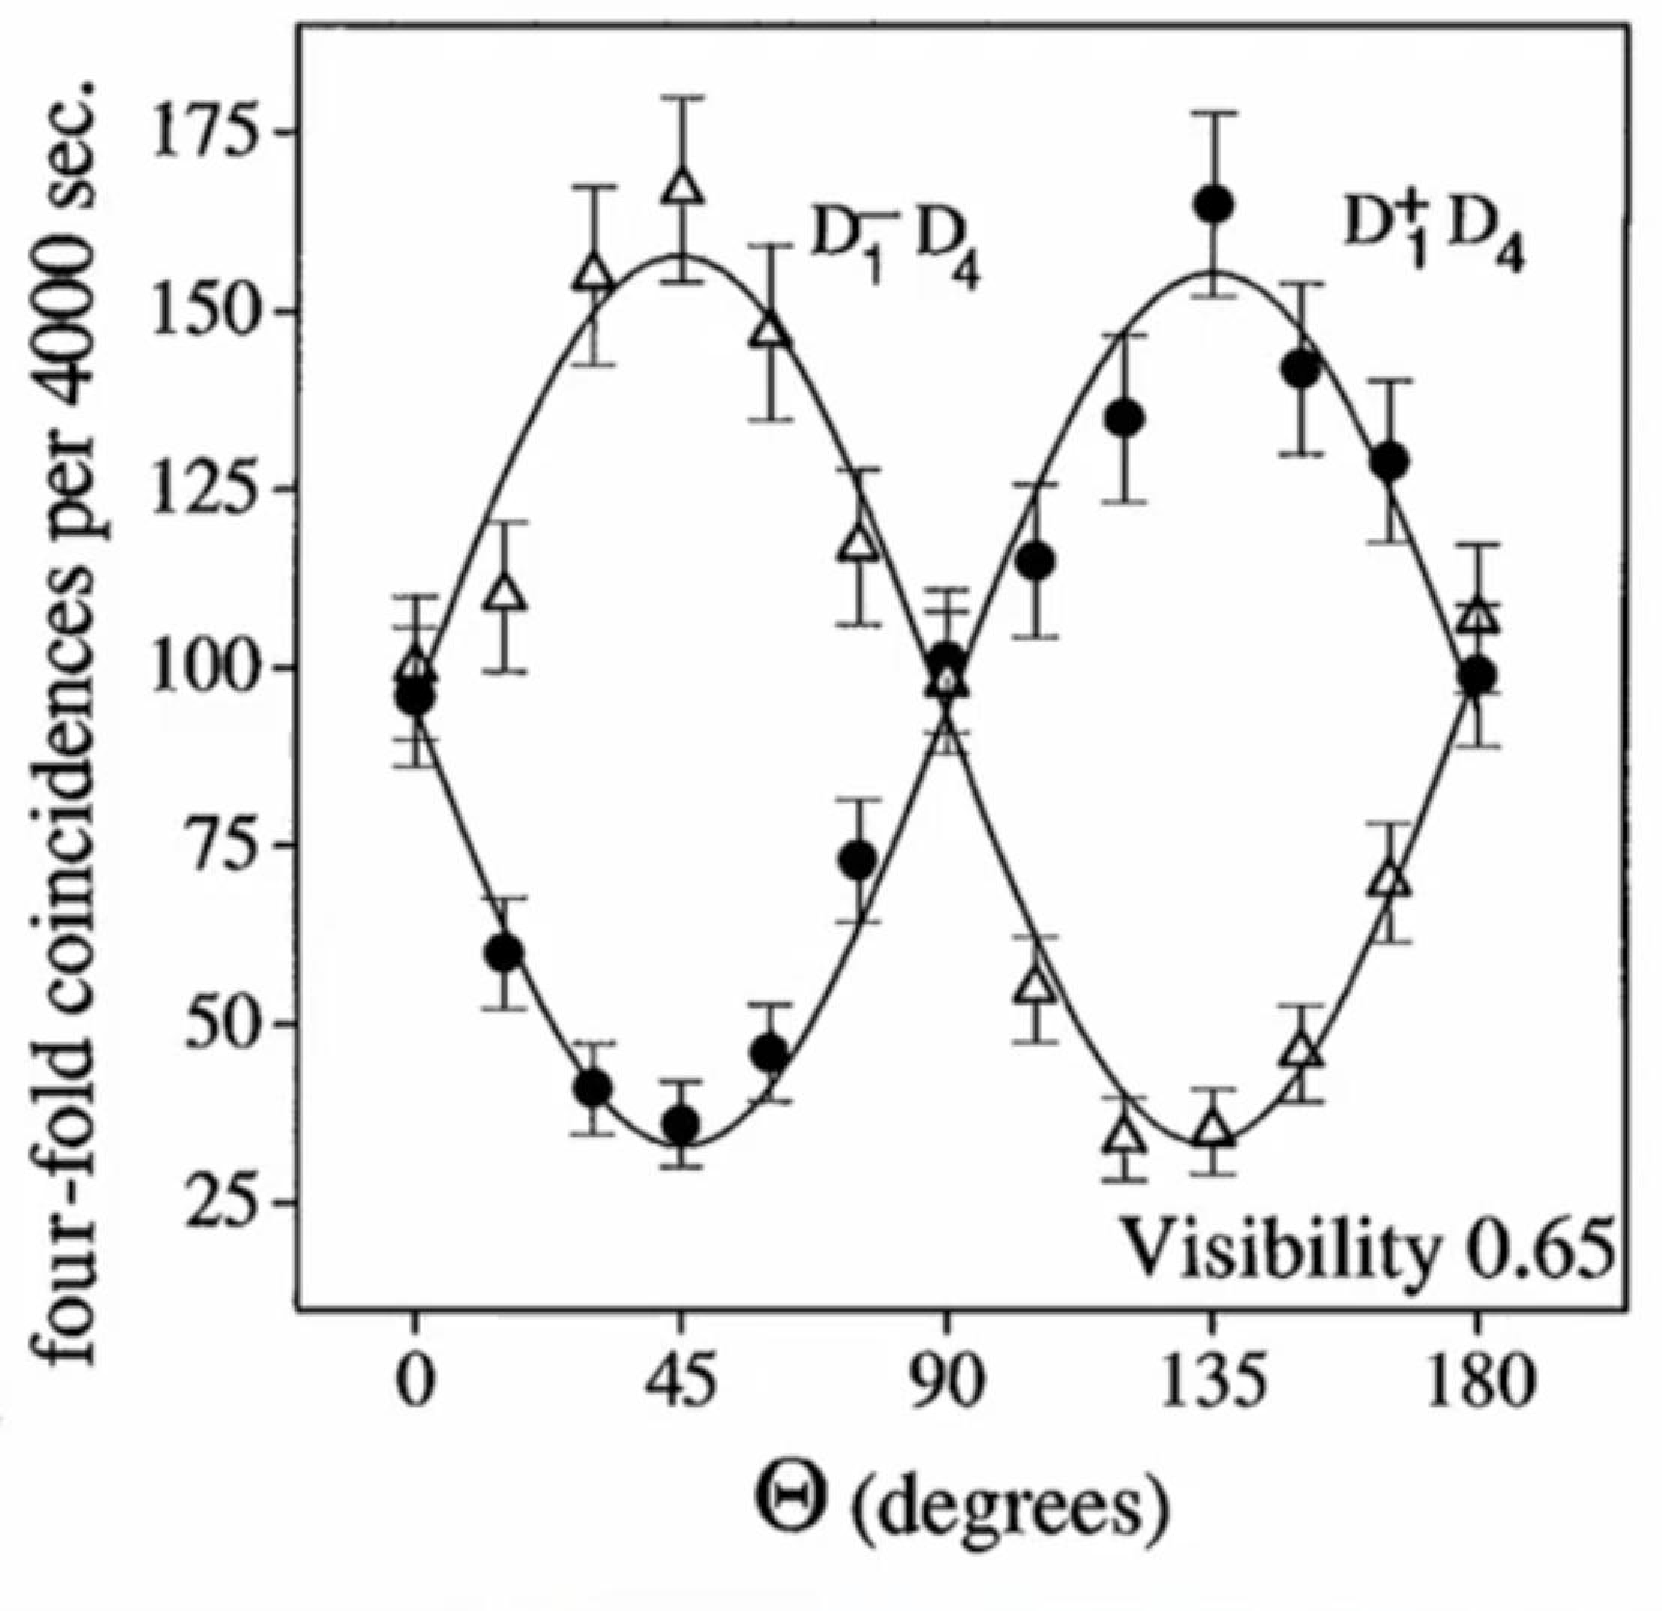
\includegraphics[width=0.6\linewidth]{images_in_pdf/16-/Grafico_102.pdf}
    \caption{Coincidence rates for entanglement swapping.}
    \label{16-entanglement-swapping}
\end{figure}

In this way, entanglement is not created by direct interaction between photons 1 and 4, but is heralded by the Bell-state measurement performed on photons 2 and 3.
Notice that there is no violation of the no-cloning theorem, because in the process of performing the Bell state measurement, \hl{the original state is itself destroyed}.

\subsection{Quantum networks}

\hl{The idea of entanglement swapping can be extended to the propagation of entanglement across many nodes}. If the same scheme is replicated for $N$ sources, the entanglement can be distributed step by step so that the first photon becomes eventually entangled with the last one. In this way, entanglement is not simply transmitted, but propagated through a network, and this \hl{can be exploited for quantum communication tasks} such as \textbf{entanglement-based quantum key distribution} or the \textbf{connection of distant quantum processors}. 

Quantum information is generated, processed, and stored locally in quantum nodes, while the nodes are linked by quantum channels that transport quantum states from site to site with high fidelity and distribute entanglement over the whole network. The natural extension of this idea is the \textbf{quantum internet}.

\subsubsection{Quantum repeaters}

In a classical communication link, losses due to absorption, scattering, and other imperfections are usually compensated by repeaters or amplifiers, which restore the signal by copying the same information. In quantum communication this is impossible, because quantum states cannot be cloned. For this reason, one needs radically new hardware, namely \textbf{quantum repeaters}, in order to build a quantum internet. In their simplest form, \hl{quantum repeaters rely on entanglement swapping}:
\begin{enumerate}
    \item The repeater first generates entanglement with two neighboring nodes, whose distance from the repeater must be short enough to allow efficient transmission through a telecom channel.
    \begin{figure}[H]
        \centering
        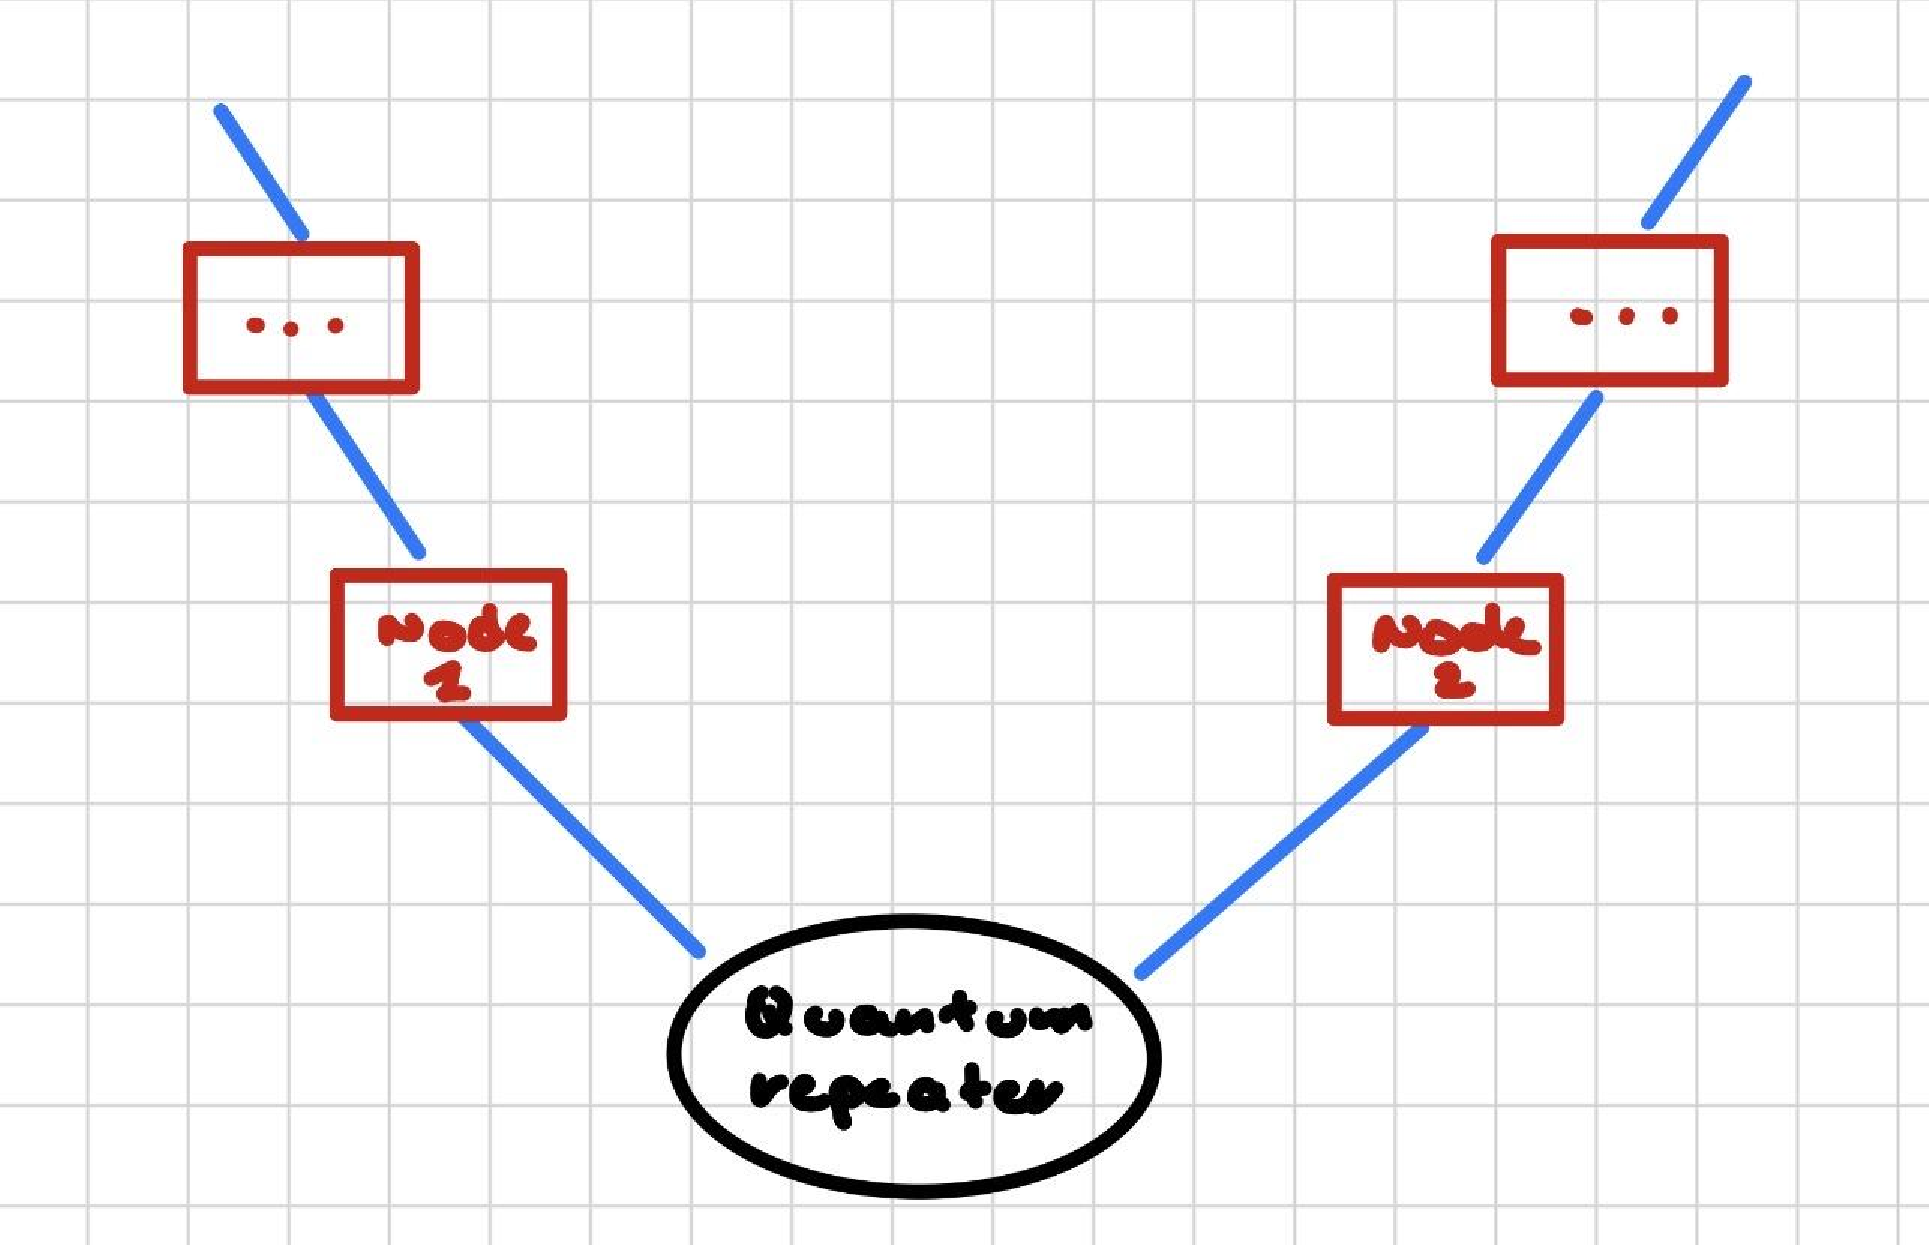
\includegraphics[width=0.6\linewidth]{images_in_pdf/16-/Grafico_103.pdf}
        \caption{Entanglement swapping in a quantum repeater.}
    \end{figure}

    \item The repeater then stores the quantum state for the time needed to establish entanglement with the next nodes in the network. This requires a \textbf{quantum memory}, which can be implemented, for instance, using long-lived spin degrees of freedom such as nuclear spins.

    \item To transmit information through a quantum network without losing coherence, a major direction of research focuses on spin-photon interfaces. These interfaces allow a quantum memory to herald the arrival of a photon and to store the associated quantum state. In this way, photon losses during transmission can be mitigated, and the stored state can later be retrieved on demand by emitting a photon carrying the same quantum information.

    A single-photon detector converts the arrival of a photon into an electrical signal, but the actual implementation of a spin-photon interface requires a much more specialized device. In semiconductor heterostructures, such as Si/Ge platforms, a two-dimensional electron gas can be formed and locally confined by electrostatic gates, creating quantum dots with single-electron control. These structures make it possible to manipulate electron spins, to store quantum information, and, in principle, to interface spin qubits with photons for teleportation, entanglement distribution, or quantum networking. However, such devices are technologically very demanding, and the realization of efficient single-photon sources and robust spin-photon interfaces remains a major experimental challenge.
\end{enumerate}

\subsection{Quantum computing overview}\label{subsec:17-quantum-computing-overview}

\subsubsection{Qubit notation exploiting binary representation}

For a general state, we already saw that we can write: 
\begin{equation*}
\ket{\psi} = a \, \ket{0}+b\, \ket{1}; \hspace{2ex} |a|^2+|b|^2 = 1
\end{equation*}

We can define the \textbf{quantum-register} as a collection of qubits; for example, the following 3-qubit register is:
\begin{equation}\label{eqn:16-5-in-binary-representation}
\ket{1}\otimes\ket{0}\otimes\ket{1} \equiv 
\ket{101} \coloneqq \ket{5}
\end{equation}

It represents $5$ in binary representation: $(5)_{10} = (101)_2$\footnote{The pedice $_{10}$ stands for base $10$ while $_{2}$ stands for base $2$.}.

If the first qubit is itself in a superposition:
\begin{equation*}
\frac{1}{\sqrt{2}}\,\bigl(\ket{0}+\ket{1}\bigr)
\end{equation*}

The register would be:
\begin{equation*}
\frac{1}{\sqrt{2}}\,
\bigl(\ket{0}+\ket{1}\bigr) \, \ket{0}\ket{1} = 
\frac{1}{\sqrt{2}}\, 
\bigl(\ket{001}+\ket{101}\bigr) = 
\frac{1}{\sqrt{2}}\, 
\bigl(\ket{1}+\ket{5}\bigr)
\end{equation*}

We obtain a simultaneous representation of two numbers. 

\question{What happens when all three qubits are in a superposition state?}{%
\begin{gather*}
\frac{1}{\sqrt{2}}\,
\bigl(\ket{0}+\ket{1}\bigr) \otimes
\frac{1}{\sqrt{2}}\,
\bigl(\ket{0}+\ket{1}\bigr) \otimes
\frac{1}{\sqrt{2}}\,
\bigl(\ket{0}+\ket{1}\bigr) =
\\
= \frac{1}{\sqrt{2^3}}\, 
\bigl(
    \ket{000}+\ket{001}+\ket{010}+\ket{011}+
    \ket{100}+\ket{101}+\ket{110}+\ket{111}
\bigr) =
\\
= \frac{1}{\sqrt{2^3}}\, 
\bigl(
    \ket{0}+\ket{1}+\ket{2}+\ket{3} +
    \ket{4}+\ket{5}+\ket{6}+\ket{7}
\bigr)
\end{gather*}

Which represents the quantum superposition of $8$ decimal numbers, this let us understand why quantum operations scale drastically computing power. The most general quantum computing register is indeed:
\begin{equation}\label{16-most-general-quantum-register}
\ket{\psi_N} = 
\bigotimes_{i=0}^{N-1} \, 
\frac{1}{\sqrt{2}} 
\bigl(
    \ket{0}_i + \ket{1}_i
\bigr) \equiv
\sum_{n=0}^{2^{N} - 1} 
\frac{1}{\sqrt{2^{N}}} \, \ket{n}
\end{equation}

where $i$ indexes the qubits in the quantum register, while $n$ is the decimal representation of the binary string (a.k.a. \emph{bitstring}) formed by the qubits. 
}

\subsubsection{Brief review of quantum computing} 

In a quantum register, information is encoded in the amplitudes of a state vector, whose description grows exponentially with the number of qubits, since \hl{an $N$-qubit system lives in a Hilbert space of dimension $2^N$}. This is the origin of the potential advantage over classical bits, whose description scales only linearly with $N$. 

\calloutinfo{%}
    The challenge is therefore to exploit this parallelism while preserving the quantum information and preventing decoherence. A quantum computer consists of a set of $N$ qubits whose state is manipulated by unitary operators, which are called \textbf{quantum gates}; a sequence of such gates forms a \textbf{quantum circuit}. 

    Through \textbf{quantum interference}, some amplitudes can be enhanced while others are canceled, and the goal is to combine these basic operations in a useful way, giving rise to \textbf{quantum algorithms}.
}

In a classical computer, a register stores bits of data and logic gates act on them; in the quantum case, the register is a state vector, and the circuit acts on qubits that may play the role of \textbf{control} and \textbf{target} qubits. More generally, \hl{a quantum computer is any device that uses quantum effects to perform a computational task}. The computation is described by a unitary transformation $U$, obtained as the product of elementary quantum logic operations, where unitary means\footnote{Un po' tardi dirlo solo all'ultimo capitolo no?}:
\begin{equation}\label{eqn:16-unitary-operator}
\hat{U}^\dagger \hat{U} = \hat{U}\hat{U}^\dagger = \mathbb{I},
\end{equation}

for example, the time-evolution operator
\begin{equation}\label{eqn:16-time-evolution-operator}
\hat{U}(t)=e^{-\frac{i}{\hbar}t\hat{H}}.
\end{equation}

Since unitary transformations are invertible, quantum computation is -- in principle -- \textbf{reversible}. A unitary operation evolves the quantum register while preserving the normalization of the state-vector, and therefore the quantum information stored in its amplitudes. 

The final step of a quantum computation is measurement, which extracts the result but is not unitary, since it projects the state onto one outcome and destroys the other components of the superposition. As a consequence, \hl{the result is probabilistic and the algorithm must often be repeated many times to obtain reliable statistics}. For this reason, quantum algorithms must be designed so that the amplitudes corresponding to incorrect answers interfere destructively, while the correct answer is amplified.

Finally, interaction with the environment leads to decoherence, which is also non-unitary and tends to destroy superposition and entanglement. This is why an important part of quantum computing research is devoted to error-correction and other protocols that protect quantum information from loss.

\subsubsection{Most remarkable single-qubit quantum logic gates}

\begin{enumerate}
    \item \textbf{Hadamard gate:} creates a superposition of the basis states
    \begin{equation}\label{eqn:16-hadamard-gate}
    \hat{H} = \frac{1}{\sqrt{2}}\, 
    \bigl[
        \ket{0}\bra{0}+\ket{0}\bra{1}+\ket{1}\bra{0}+\ket{1}\bra{1}
    \bigr] = 
    \frac{1}{\sqrt{2}}\, 
    \begin{pmatrix}
        1 & 1\\ 1 &-1
    \end{pmatrix}
    \end{equation}

    When applied to either state $\ket{0}$ or $\ket{1}$ leads to an equal superposition of both states. Being at the same time self-adjoint (a.k.a. \textbf{hermitian}) and unitary, it is its own inverse; thus can turn superposition states again into basis states:
    \begin{equation}
    \hat{H}\, 
    \frac{1}{\sqrt{2}}\, 
    \begin{pmatrix}
        1\\1 
    \end{pmatrix} =  \frac{1}{\sqrt{2}}\,\frac{1}{\sqrt{2}}\, \begin{pmatrix}
        1 & 1\\ 1 &-1
    \end{pmatrix}\, \begin{pmatrix}
        1\\1 
    \end{pmatrix} = \frac{1}{2}\, \begin{pmatrix}
        2\\0
    \end{pmatrix} = \begin{pmatrix}
        1\\0
    \end{pmatrix}.
    \end{equation}

    Considering Bloch sphere's representation, changing the amplitude of the qubit corresponds to operating some rotations on its position:
    \begin{enumerate}
        \item Rotation of $\pi$ about the $z$-axis;
        \item Rotation of $\frac{\pi}{2}$ about the $y$-axis.
    \end{enumerate}

    \item \textbf{X-gate:} also referred to as \textbf{not-gate}, since it switches $\ket{0}$ with $\ket{1}$ and vice versa:
    \begin{equation}\label{eqn:16-x-gate}
    \hat{X} = 
    \ket{1}\bra{0}+\ket{0}\bra{1} = 
    \begin{pmatrix}
        0 &1\\1&0
    \end{pmatrix}
    \end{equation}

    It corresponds to a rotation of $\pi$ about the $x$-axis.

    \item \textbf{Z-gate:} flips the sign of $\ket{1}$, leaving $\ket{0}$ unchanged
    \begin{equation}\label{eqn:16-z-gate}
    \hat{Z} = \ket{0}\bra{0}-\ket{1}\bra{1} = \begin{pmatrix}
        1 &0\\0&-1
    \end{pmatrix}
    \end{equation}

    It corresponds to a rotation of $\pi$ about the $z$-axis.

    \item \textbf{Y-gate:} change $\ket{0}\to i\, \ket{1}$ and $\ket{1} \to -i\, \ket{0}$
    \begin{equation}\label{eqn:16-y-gate}
    \hat{Y} = i\, \ket{1}\bra{0}-i\,\ket{0}\bra{1} = \begin{pmatrix}
        0 &-i\\i&0
    \end{pmatrix}
    \end{equation}

    It corresponds to a rotation of $\pi$ about the $y$-axis.
\end{enumerate}

As said, all these gates can be thought as some rotations on the Bloch sphere; without any formalism, we can say that they are generalized by the generic rotation:
\begin{equation}\label{eqn:16-generic-rotation}
    \hat{R}_{\phi} = \ket{0}\bra{0}+e^{i\phi}\, \ket{1}\bra{1}
\end{equation}

\subsubsection{Two-qubit gates overview and controlled operations}

The gates which operates on two or more qubits are called \textbf{controlled operations}. Suppose to have a 2 input q-bits one is control and the other is target, the gate has no effect on the control q-bit, but performs a unitary operation on the target q-bit conditionally on the state of the control q-bit.
\textbf{C-NOT gate:} (controlled-not)
\begin{equation}\label{eqn:16-cnot-gate}
\hat{C} = 
\ket{00}\bra{00} + \ket{01}\bra{01} +
\ket{10}\bra{11} + \ket{11}\bra{10} = 
\begin{pmatrix}
    1&0&0&0\\ 
    0&1&0&0\\
    0&0&0&1\\
    0&0&1&0
\end{pmatrix}
\end{equation}

If the control state is $\ket{0}$ the target state remains unchanged, while if the control state is $\ket{1}$ the target state flips whatever its initial state is. 
This gate can be written in a symbolic form as:
\begin{equation}\label{eqn:16-cnot-circuit}
\begin{quantikz}
\lstick{$\ket{c}$} & \ctrl{1} & \rstick{$\ket{c}$} \\
\lstick{$\ket{t}$} & \targ{}  & \rstick{$\ket{t \oplus c}$}
\end{quantikz}
\end{equation}

Where $\oplus$ is addition modulo $2$ \footnote{For a single-qubit state $\ket{t}$, $t$\in\{0,1\}; if $c=0$ nothing happens, whereas if $c=1$ the possibile outcomes are: $0\oplus 1 = 1$ and $1\oplus 1 = 0$}.


\subsection{Optical implementation of quantum gates}\label{subsec:17-optical-implementation-of-quantum-gates}

\question{How can we implement this with optical schemes?}{%
Quantum information is encoded onto modes occupied by single photons, which are manipulated using linear optical components such as B.S., phase shifters, etc...
}

\subsubsection{Hadamard gate through a half-wave plate}

Let's start with \textbf{Hadamard gate}: the simplest optical object that realizes it is a half-wave plate, an optical device that alters the polarization of light (here by \qty{45}{\degree}).

\begin{figure}[H]
    \centering
    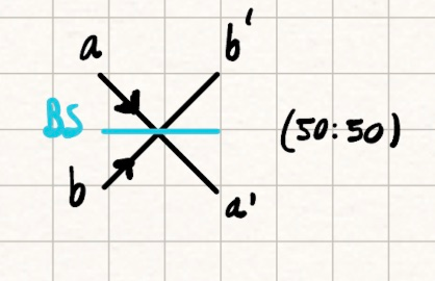
\includegraphics[width=0.4\linewidth]{images_in_pdf/17-/17-hadamard-bs.pdf}
    \caption{Hadamard gate through a half-wave plate.}
\end{figure}

\begin{equation}\label{eqn:17-dual-rail-realization-1}
\begin{cases}
    \hat{a}' = \frac{1}{\sqrt{2}}\, (\hat{a}+\hat{b})\\
    \hat{b}' = \frac{1}{\sqrt{2}}\, (\hat{a}-\hat{b})
\end{cases} \implies \hspace{2ex}
\begin{cases}
    \hat{a} = \frac{1}{\sqrt{2}}\, (\hat{a}'+\hat{b}')\\
    \hat{b} = \frac{1}{\sqrt{2}}\, (\hat{a}'-\hat{b}')
\end{cases}
\end{equation}

\subsubsection{Hadamard gate through a B.S.}

We take in consideration the \textbf{dual rail realization} (i.e. an architecture where a single bit, called \say{logical state} is represented by two physical signals) through a B.S. 

The computational states $\ket{0}$ and $\ket{1}$ are composed by the product of two states:
\begin{equation}\label{eqn:17-dual-rail-realization-2}
\ket{0} \coloneqq \ket{0}_a\ket{1}_b
\hspace{1ex} \land \hspace{1ex}
\ket{1} \coloneqq \ket{1}_a\ket{0}_b
\end{equation}

Notice that, by themselves, the vacuum and single-photon states do not compose the computational basis; it is their product that gives us the states on which we operate.

The two input modes are labeled $a$ and $b$, while the output modes are labeled $a'$ and $b'$. On our logic states, the B.S. transformation $\hat{U}_{\text{B.S.}}$ acts as:
\begin{align}
\hat{U}_{\text{B.S.}} \ket{0}_a \ket{1}_b &= 
\frac{1}{\sqrt{2}} 
\bigl( 
    \ket{0}_{a'}\ket{1}_{b'} + \ket{1}_{a'}\ket{0}_{b'} 
\bigr) = \nonumber \\
&= \frac{1}{\sqrt{2}}
\bigl(
    \ket{01} + \ket{10}
\bigr); \label{eqn:17-bs-transformation-01} \\[2ex]
%
\hat{U}_{\text{B.S.}} \ket{1}_a \ket{0}_b 
&= \frac{1}{\sqrt{2}} 
\bigl( 
    \ket{1}_{a'}\ket{0}_{b'} - \ket{0}_{a'}\ket{1}_{b'} 
\bigr) \nonumber = \\
&= \frac{1}{\sqrt{2}} 
\bigl( 
    \ket{10} - \ket{01} 
\bigr). \label{eqn:17-bs-transformation-10}
\end{align}


\subsubsection{C-NOT gate through linear optics}

Let us implement a \textbf{linear optical C-NOT} gate exploiting \textbf{polarizing beam splitters (p.B.S.)}\footnote{A polarizing beam splitter is a device that separates light into two components based on their polarization, contrary to the 50:50 variant that separates light into parts of equal intensity.}, unbalanced beam splitters (u.B.S.), half-wave plates (H.W.P.) and \emph{post-selection}.
\begin{figure}[H]
    \centering
    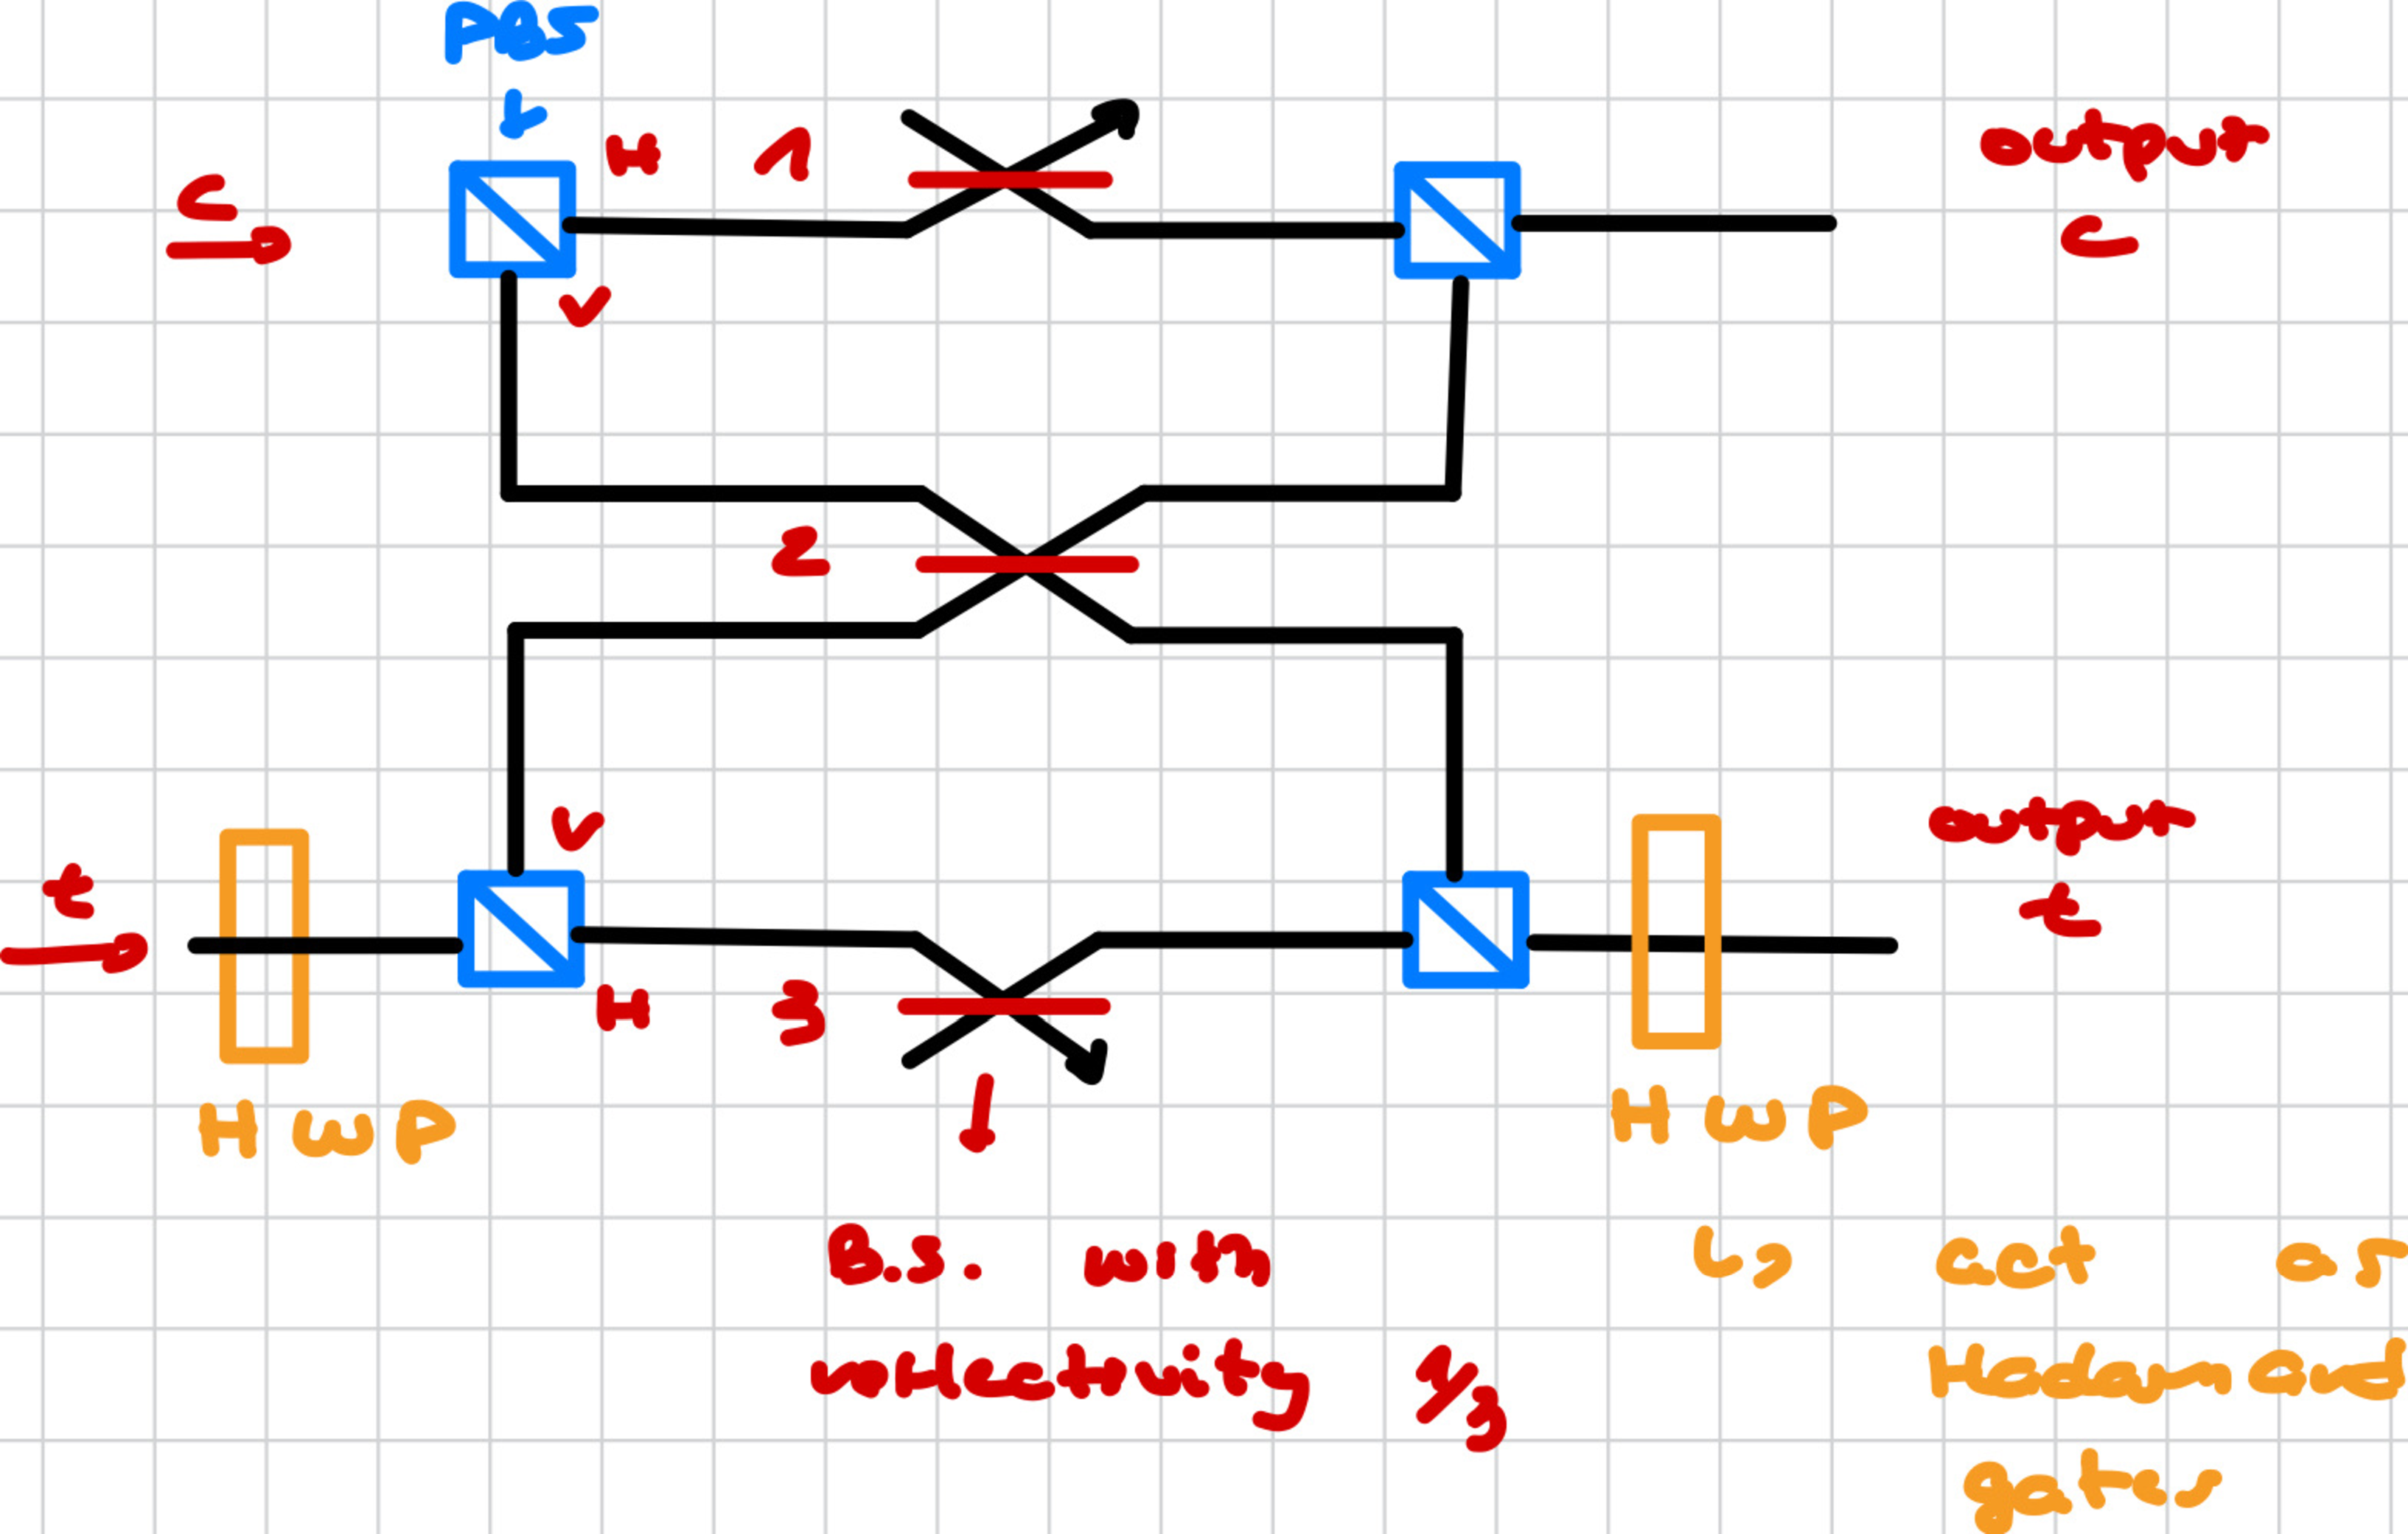
\includegraphics[width=0.6\linewidth]{images_in_pdf/17-/17-cnot-lin-opt.pdf}
    \caption{C-NOT gate through p.B.S.s, u.B.S.s, and H.W.P.s.}
\end{figure}

\begin{enumerate}
\item The \textbf{control qubit} approaches a \emph{polarizing beam splitter} \hl{which produces a horizontal (transmitted) and a vertical (reflected) component};

\item The \textbf{target qubit} approaches another \emph{polarizing beam splitter} \hl{which also produces a horizontal and a vertical component};

\item The \emph{transmitted component} of the control qubit goes to an \textbf{unbalanced B.S.} with a reflectivity of $\frac{1}{3}$ (hence $\tran=\frac{2}{3}$), then follows a path to another polarizing beam splitter, where it can give only a single output; the same happens for the transmitted part of the target qubit;

\item Both \emph{reflected components} are \textbf{mixed} in another unbalanced B.S. with the same reflectivity; the upper one goes to a polarizing beam splitter and then to the output of the control qubit, while the lower one goes to another polarizing beam splitter;

\item Now, \hl{only for the target qubit}, we add a \textbf{half-wave plate} \emph{before} the first polarizing beam splitter and \emph{another after} the second one, which act as Hadamard gates.
\end{enumerate}

To study the C-NOT behavior of this apparatus, we use \textbf{dual-rail logic}. We use a particular notation, where $c$ and $t$ will stand for the control and target qubits, respectively; a pedice $H$ or $V$ will indicate the polarization considered. In this sense, we will refer to the states $\ket{H}_c$ and $\ket{V}_c$ as:

\begin{equation}
\ket{H}_c \coloneqq \ket{0} \mapsto  
\begin{cases}
    \ket{1}_{c_H}\\
    \ket{0}_{c_V}
\end{cases} 
\end{equation}

\begin{equation}
\ket{V}_c \coloneqq \ket{1} \mapsto  
\begin{cases}
    \ket{0}_{c_H}\\
    \ket{1}_{c_V}
\end{cases} 
\end{equation}

The same will hold for the target qubit.

\calloutinfo{%
    To stress it again, a horizontal polarization corresponds to the logical state $\ket{0}$, while a vertical polarization corresponds to the logical state $\ket{1}$. The C-NOT gate should then flip the polarization of the target qubit if the control qubit's polarization is vertical, while leaving it unchanged if the control qubit's polarization is horizontal.
}

Let's unpack the behavior of this system by considering the possible input states.

\calloutwarn{%
    We only consider events where photons arrive at both the target and control outputs simultaneously (clicking the outputs simultaneously); this is called \textbf{post-selection}, i.e.: discarding all outcomes that do not satisfy the chosen criteria. This means that we do not take into account the events in which photons are transmitted by the first and third u.B.S., since it would mean the photons are exiting the system. At the same time, we also discard the events where the second u.B.S. reflects one photon while transmitting the other, since it would mean that they are exiting from the same output port.
} 

\begin{itemize}

\item[\textbf{CASE \Rnum{1}:}] \hl{both input photons are horizontally polarized}, $\ket{H}_c$ and $\ket{H}_t$. The target qubit passes through the half-wave plate, which acts as a Hadamard transformation sending it to a superposition of horizontal and vertical polarization:
\begin{equation}
\ket{H}_c\ket{H}_t 
\stackrel{\text{\tiny{H.W.P.}}}{\longrightarrow} 
\ket{H}_c \, 
\otimes
\frac{1}{\sqrt{2}}\, 
\bigl( 
    \ket{H}_t+\ket{V}_t
\bigr)
\end{equation}

When our input photons enter their first p.B.S.:

\begin{itemize}
    \item The control qubit has a definite \emph{horizontal} polarization, hence exits the p.B.S. on the top path, then gets reflected by the first u.B.S.;
    \item The target qubit was put in a superposition so, exiting the p.B.S., it can either take the middle path (making it \emph{vertical}) and get reflected by the second u.B.S. or choose the bottom path (making it \emph{horizontal}) and get reflected by the third u.B.S.
\end{itemize}

Overall, requiring two u.B.S. reflections, the amplitude of the successful components is reduced by a factor of: $\frac{1}{\sqrt{3}}\, \frac{1}{\sqrt{3}}= \frac{1}{3}$.

The output state is then:
\begin{equation}
\frac{1}{3}\, \ket{H}_c \,
\otimes
\frac{1}{\sqrt{2}} \,
\bigl( \ket{H}_t+\ket{V}_t\bigr)
\end{equation}

But now we have a second H.W.P. acting on the target qubit, making it go back from a superposition to a vertical state: $\tfrac{1}{\sqrt{2}}  \, \bigl( \ket{H}_t+\ket{V}_t\bigr)\to \ket{H}_t$.
\begin{equation}
\text{Output} = \frac{1}{3}\, \ket{H}_c\, \ket{H}_t
\end{equation}

We obtain the initial state, only with a different amplitude; this is the expected behavior of a C-NOT gate, since the control qubit is horizontal and therefore does not flip the target qubit's polarization.

\item[\textbf{CASE \Rnum{2}:}] control is horizontal and target is vertical: $\ket{H}_c\ket{V}_t$. This case is completely analogous to the previous one, and the same output is obtained.

\item[\textbf{CASE \Rnum{3}:}] control is vertical and target is horizontal: $\ket{V}_c\ket{H}_t$.

The target qubit passes through the half-wave plate, which acts as a Hadamard transformation:
\begin{equation}
\ket{V}_c\ket{H}_t 
\stackrel{\text{\tiny{H.W.P.}}}{\longrightarrow}
\ket{V}_c 
\otimes
\frac{1}{\sqrt{2}}\,
\bigl( \ket{H}_t+\ket{V}_t\bigr)
\end{equation}

\begin{itemize}
    \item The control qubit has a definite \emph{vertical} polarization, hence exits the p.B.S. on the middle path; from here, it can either be reflected or transmitted by the second u.B.S.;
    \item The target qubit was put in a superposition so, exiting the p.B.S., it can either take the middle path (making it \emph{vertical}) and then can be reflected or transmitted as well by the second u.B.S. [case \Rnum{3}\hspace{0.2ex}a.]; or choose the bottom path (making it \emph{horizontal}) where it has to be reflected by the third u.B.S. [case \Rnum{3}\hspace{0.2ex}b.];
\end{itemize}

\begin{itemize}

\item[\textbf{\Rnum{3}\hspace{0.2ex}b.}] If the target photon follows the bottom path, the coincidence is realized only if both photons are reflected by the second and third u.B.S., respectively. This simply leads to a reduction of the initial amplitude by $\frac{1}{3}$, leaving the target qubit unaltered in $\ket{H}_t$.

\item[\textbf{\Rnum{3}\hspace{0.2ex}a.}] If instead the target photon follows the middle path, we have two possible scenarios -- both in which target photon's polarization it's swapped to $\ket{V}_t$ -- involving the interface at the second u.B.S.:

\begin{enumerate}
    \item \hl{Both photons are \textbf{reflected}}: control photon is detected by the upper detector, while the target photon is detected by the lower detector; this leads to a reduction of the initial amplitude by $\frac{1}{3}$.
    
    \item \hl{Both photons are \textbf{transmitted}}: control photon is detected by the lower detector, while the target photon is detected by the upper detector; the final amplitude results multiplied by $-\frac{2}{3}$.
\end{enumerate}

\calloutwarn{%
    \textbf{Caution:} the photons are indistinguishable, there's no way to know which photon was detected by which detector! 
}

Given the indistinguishability of the photons, we must consider the total amplitude of the two sub-processes: $\frac{1}{3}-\frac{2}{3} = -\frac{1}{3}$. 

\end{itemize}

We now are left with a superposition of two target outcomes: a $\ket{H}_t$ from the \textbf{\Rnum{3}\hspace{0.2ex}b.} case and $\ket{V}_t$ from the \textbf{\Rnum{3}\hspace{0.2ex}a.} case, with a relative minus sign:

\begin{equation}\label{eqn:17-cnot-case-3-pre-hwp}
\frac{1}{\sqrt{2}}\ket{V}_c\, 
\otimes
\frac{1}{3}\,
\bigl(\ket{H}_t-\ket{V}_t\bigr)
\end{equation}

After the target qubit passes through the second half-wave plate, its superposition state is sent back to $\ket{V}_t$, and we finally obtain:
\begin{equation}
\frac{1}{\sqrt{2}}\ket{V}_c\, 
\otimes
\frac{1}{3}\,
\bigl(\ket{H}_t-\ket{V}_t\bigr)
\stackrel{\text{\tiny{H.W.P.}}}{\longrightarrow}
\frac{1}{3}
\ket{V}_c \ket{V}_t
\end{equation}

\calloutinfo{%
    The minus sign in the transmission amplitude appears because of a really good reason.
}


Overall, the probability of success (i.e. the fraction of photons that successfully implement the C-NOT operation) is:
\begin{equation}
\frac{1}{3}\, \frac{1}{3} = \frac{1}{9}
\end{equation}

This is very low; we lose a large number of photons \hl{primarily due to post-selection}. For this reason, alternative realizations exist that attempt to make this system more efficient.

\end{itemize}
 
Another approach currently being explored is to use a generic entangled state called a \textbf{cluster state}.

\subsection{Boson sampling}\label{subsec:17-boson-sampling}

Boson sampling is a sampling problem based on indistinguishable photons propagating through a large linear-optical network. In the occupation-number encoding of the photonic modes, one injects $N$ single photons into a device with $M$ modes, with $M \gg N$ in order to reduce the probability of collisions, i.e. the occurrence of more than one photon in the same output mode. The \hl{photons are mixed by beam splitters and phase shifters}, and the output modes are measured by photon detectors. 

\calloutinfo{%
    The goal is to \textbf{predict how the photons are distributed} at the output of the interferometer. Because of multi-particle interference, the resulting probability distribution is extremely complex and is believed to be intractable for classical computers.
}

We can define a \textbf{boson sampler} as a large multi-path interferometer. In the Heisenberg picture, the output mode operators are related to the input ones by
\begin{equation}
\hat{b}_j=\sum_{k=1}^{M} U_{jk}\hat{a}_k,
\end{equation}

where $\hat{a}_k$ denotes the input mode operator and $U_{jk}$ is the unitary matrix describing the optical network. Since real devices are not perfect, losses may occur; for this reason, one often uses \textbf{post-selection} and keeps only the events in which all $N$ photons are detected at the output.

For collision-free events, \hl{the probability of a given output pattern is determined by the \textbf{permanent} of a suitable sub-matrix of $U$}. For example, if $N=2$ and $M=4$, and we are interested in the output configuration where a single photon is detected at first (\Rnum{1}) and third (\Rnum{3}) output modes:
\begin{equation}
\ket{1}_\text{\Rnum{1}}\otimes\ket{0}_\text{\Rnum{2}}\otimes
\ket{1}_\text{\Rnum{3}}\otimes\ket{0}_\text{\Rnum{4}}
\coloneqq
\vec{n}=(1,0,1,0),
\end{equation}

the corresponding probability is obtained from the $2\times 2$ sub-matrix of $U$ formed by selecting the input and output modes occupied by the photons. In the collision-free case,
\begin{equation}
P(\vec{n})=
\left[
    \operatorname{Per} ([U]_{1_{M\times\vec{n}}})^2
\right]
\end{equation}

where $U_{1_{M\times\vec{n}}}$ is the sub-matrix obtained by selecting the first $M$ columns and $\vec{n}$ rows of $U$. The permanent of a $2\times 2$ matrix is
\begin{equation}
\operatorname{Per}\begin{pmatrix}
a & b\\
c & d
\end{pmatrix}=ad+bc.
\end{equation}

\hl{The main difficulty is that the permanent is much harder to compute than the determinant}: in general, its exact classical evaluation scales exponentially with the matrix size and is a $\#P$-hard problem. A second difficulty is that the number of possible output configurations grows very rapidly with $M$ and $N$. In the collision-free regime, the number of output patterns scales as
\begin{equation}\label{eqn:17-binomial-coefficient}
\binom{M}{N}=\frac{M!}{N!(M-N)!},
\end{equation}

which becomes enormous already for moderately large systems. For this reason, large boson-sampling devices are very difficult to simulate or fully characterize classically \cite{art:Zhong-2020-quantum-advantage}.

\subsection{Today's Challenges: Decoherence and Error Correction}

A quantum system is never perfectly isolated, because it must interact with the environment and with external control fields in order to be manipulated and measured. As a consequence, decoherence becomes one of the main limitations for quantum computation. The dominant sources of noise are thermal fluctuations, coupling to phonons, fluctuating electromagnetic fields, charge noise, and other uncontrolled interactions, all of which can destroy phase coherence and reduce the visibility of quantum interference. In practice, \hl{both relaxation and dephasing processes limit the number of operations} (i.e., the number of layers of gates in a quantum circuit) that can be performed before the state is lost. 

A rough estimate of the available computational depth is
\begin{equation}\label{eqn:17-computational-depth}
M = \frac{T_{\text{Dephasing}}}{T_{\text{gate}}}
\end{equation}

where $T_{\text{Dephasing}}$ is the dephasing time and $T_{\text{gate}}$ is the duration of a single gate operation.

\hl{To overcome these limitations, one introduces \textbf{quantum error correction}}. A simple parity check on the data qubits does not work directly, because measuring the qubits would collapse the quantum state and destroy the information we want to protect. 

Instead, one encodes the logical information into a larger entangled register and \hl{uses auxiliary \textbf{ancilla} qubits to extract an error syndrome without destroying the logical state} (\emph{non-demolition measurements}) itself or use directly a second register called \say{sacrificial} register to check the fidelity of data. The syndrome can then be processed by a correction algorithm.

If this procedure is implemented consistently, one obtains \textbf{fault-tolerant quantum computing}. The price to pay is a large overhead: more physical qubits, more gates, and a reduction in speed due to the extra correction steps. This \hl{overhead is one of the major challenges in scaling quantum computers}.

The current generation of devices is usually described as belonging to the \textbf{Noisy Intermediate-Scale Quantum (NISQ)} era: \hl{quantum processors already exist, but they are not yet large or clean enough to support fully fault-tolerant computation} or to guarantee a universal quantum advantage for arbitrary tasks. A further practical difficulty is that many quantum platforms require a large number of optical or electronic components that must be precisely aligned and stabilized. For this reason, integrated photonic chips and semiconductor-based architectures are being actively developed as a route toward scalable quantum technologies \cite{art:Arute-2019-quantum-supremacy,art:Acharya-2024-error-correction}.

\vspace{2ex}

\emph{The end.}

\listoffigures

\end{document} 